\documentclass[twoside]{book}

% Packages required by doxygen
\usepackage{fixltx2e}
\usepackage{calc}
\usepackage{doxygen}
\usepackage[export]{adjustbox} % also loads graphicx
\usepackage{graphicx}
\usepackage[utf8]{inputenc}
\usepackage{makeidx}
\usepackage{multicol}
\usepackage{multirow}
\PassOptionsToPackage{warn}{textcomp}
\usepackage{textcomp}
\usepackage[nointegrals]{wasysym}
\usepackage[table]{xcolor}

% Font selection
\usepackage[T1]{fontenc}
\usepackage[scaled=.90]{helvet}
\usepackage{courier}
\usepackage{amssymb}
\usepackage{sectsty}
\renewcommand{\familydefault}{\sfdefault}
\allsectionsfont{%
  \fontseries{bc}\selectfont%
  \color{darkgray}%
}
\renewcommand{\DoxyLabelFont}{%
  \fontseries{bc}\selectfont%
  \color{darkgray}%
}
\newcommand{\+}{\discretionary{\mbox{\scriptsize$\hookleftarrow$}}{}{}}

% Page & text layout
\usepackage{geometry}
\geometry{%
  a4paper,%
  top=2.5cm,%
  bottom=2.5cm,%
  left=2.5cm,%
  right=2.5cm%
}
\tolerance=750
\hfuzz=15pt
\hbadness=750
\setlength{\emergencystretch}{15pt}
\setlength{\parindent}{0cm}
\setlength{\parskip}{3ex plus 2ex minus 2ex}
\makeatletter
\renewcommand{\paragraph}{%
  \@startsection{paragraph}{4}{0ex}{-1.0ex}{1.0ex}{%
    \normalfont\normalsize\bfseries\SS@parafont%
  }%
}
\renewcommand{\subparagraph}{%
  \@startsection{subparagraph}{5}{0ex}{-1.0ex}{1.0ex}{%
    \normalfont\normalsize\bfseries\SS@subparafont%
  }%
}
\makeatother

% Headers & footers
\usepackage{fancyhdr}
\pagestyle{fancyplain}
\fancyhead[LE]{\fancyplain{}{\bfseries\thepage}}
\fancyhead[CE]{\fancyplain{}{}}
\fancyhead[RE]{\fancyplain{}{\bfseries\leftmark}}
\fancyhead[LO]{\fancyplain{}{\bfseries\rightmark}}
\fancyhead[CO]{\fancyplain{}{}}
\fancyhead[RO]{\fancyplain{}{\bfseries\thepage}}
\fancyfoot[LE]{\fancyplain{}{}}
\fancyfoot[CE]{\fancyplain{}{}}
\fancyfoot[RE]{\fancyplain{}{\bfseries\scriptsize Generated by Doxygen }}
\fancyfoot[LO]{\fancyplain{}{\bfseries\scriptsize Generated by Doxygen }}
\fancyfoot[CO]{\fancyplain{}{}}
\fancyfoot[RO]{\fancyplain{}{}}
\renewcommand{\footrulewidth}{0.4pt}
\renewcommand{\chaptermark}[1]{%
  \markboth{#1}{}%
}
\renewcommand{\sectionmark}[1]{%
  \markright{\thesection\ #1}%
}

% Indices & bibliography
\usepackage{natbib}
\usepackage[titles]{tocloft}
\setcounter{tocdepth}{3}
\setcounter{secnumdepth}{5}
\makeindex

% Hyperlinks (required, but should be loaded last)
\usepackage{ifpdf}
\ifpdf
  \usepackage[pdftex,pagebackref=true]{hyperref}
\else
  \usepackage[ps2pdf,pagebackref=true]{hyperref}
\fi
\hypersetup{%
  colorlinks=true,%
  linkcolor=blue,%
  citecolor=blue,%
  unicode%
}

% Custom commands
\newcommand{\clearemptydoublepage}{%
  \newpage{\pagestyle{empty}\cleardoublepage}%
}

\usepackage{caption}
\captionsetup{labelsep=space,justification=centering,font={bf},singlelinecheck=off,skip=4pt,position=top}

%===== C O N T E N T S =====

\begin{document}

% Titlepage & ToC
\hypersetup{pageanchor=false,
             bookmarksnumbered=true,
             pdfencoding=unicode
            }
\pagenumbering{roman}
\begin{titlepage}
\vspace*{7cm}
\begin{center}%
{\Large event-\/driven }\\
\vspace*{1cm}
{\large Generated by Doxygen 1.8.11}\\
\end{center}
\end{titlepage}
\clearemptydoublepage
\tableofcontents
\clearemptydoublepage
\pagenumbering{arabic}
\hypersetup{pageanchor=true}

%--- Begin generated contents ---
\chapter{Main Page}
\label{index}\hypertarget{index}{}$\vert$ Read the \href{http://robotology-playground.github.io/event-driven/doxygen/doc/html/index.html}{\tt Documentation} $\vert$ Download the \href{https://github.com/robotology-playground/event-driven}{\tt Code} $\vert$

\href{https://youtu.be/xS-7xYRYSLc}{\tt }  Click the thumbnail to watch the \href{https://youtu.be/xS-7xYRYSLc}{\tt video}!

\section*{The event-\/driven Y\+A\+RP Project}

Libraries that handle neuromorphic sensors, such as the dynamic vision sensor, installed on the i\+Cub can be found here, along with algorithms to process the event-\/based data. Examples include, optical flow, corner detection and ball detection. Demo applications for controlling the robot based on event input are also found here.

\subsection*{Libraries}

\subsection*{Modules}


\begin{DoxyItemize}
\item {\bfseries Optical Flow} -- an estimate of object velocity in the visual plane is given by the rate at which the spatial location of events change over time. Such a signal manifests as a manifold in the spatio-\/temporal event space. Local velocity can be extracted by fitting planes to these manifolds. The {\ttfamily ev\+::v\+Flow} module converts the ED camera output {\ttfamily \hyperlink{classev_1_1AddressEvent}{ev\+::\+Address\+Event}} to {\ttfamily \hyperlink{classev_1_1FlowEvent}{ev\+::\+Flow\+Event}}.
\item {\bfseries Cluster Tracking} -- The movement of an object across the visual field of an ED camera produces a detailed, unbroken trace of events. Local clusters of events can be tracked by updating a tracker position as new events are observed that belong to the same trace. The spatial distribution of the events can be estimated with a Gaussian distribution. The cluster centre and distribution statistics is output from the {\ttfamily ev\+::v\+Cluster} module as a {\ttfamily \hyperlink{classev_1_1GaussianAE}{ev\+::\+Gaussian\+AE}} event.
\item {\bfseries Corner Detection} -- using an event-\/driven Harris algorithm, the full event stream is filtered to contain only the events falling on the corners of objects or structure in the scene. Corner events are useful to avoid the aperture problem and to reduce the data stream to informative events for further processing. Compared to a traditional camera, the ED corner algorithm requires less processing. {\ttfamily ev\+::v\+Corner} converts {\ttfamily \hyperlink{classev_1_1AddressEvent}{ev\+::\+Address\+Event}} to {\ttfamily \hyperlink{classev_1_1LabelledAE}{ev\+::\+Labelled\+AE}}.
\item {\bfseries Circle Detection} -- detection of circular shapes in the event stream can be performed using an ED Hough transform. As the camera moves on a robot, many background events clutter the detection algorithm. The {\ttfamily ev\+::v\+Circle} module reduces the false positive detections by using optical flow information to provide a more accurate understanding of only the most up-\/to-\/date spatial structure. {\ttfamily ev\+::v\+Circle} accepts {\ttfamily \hyperlink{classev_1_1AddressEvent}{ev\+::\+Address\+Event}} and {\ttfamily \hyperlink{classev_1_1FlowEvent}{ev\+::\+Flow\+Event}} and outputs {\ttfamily \hyperlink{classev_1_1GaussianAE}{ev\+::\+Gaussian\+AE}}.
\item {\bfseries Particle filtering} -- probabilistic filtering is used to provide a robust tracking over time. The particle filter is robust to variations in speed of the target by also sampling within the temporal dimension. A observation likelihood function that responds to a circular shape was developed to instigate a comparison with the Hough transform. The tracking position is output as {\ttfamily \hyperlink{classev_1_1GaussianAE}{ev\+::\+Gaussian\+AE}}. Future work involves adapting the filter to respond to different target shapes, and templates learned from data.
\end{DoxyItemize}

\subsection*{Applications for the i\+Cub Humanoid Robot}

\subsection*{How to Install\+:}


\begin{DoxyEnumerate}
\item Install \href{https://github.com/robotology/yarp}{\tt Y\+A\+RP} and \href{https://github.com/robotology/icub-contrib-common}{\tt icub-\/contrib-\/common} following these \href{http://wiki.icub.org/wiki/Linux:Installation_from_sources}{\tt instructions}.
\item Clone event-\/driven and install as an icub-\/contrib module.
\end{DoxyEnumerate}

\subsection*{References}

Glover, A., and Bartolozzi C. (2016) {\itshape Event-\/driven ball detection and gaze fixation in clutter}. In I\+E\+E\+E/\+R\+SJ International Conference on Intelligent Robots and Systems (I\+R\+OS), October 2016, Daejeon, Korea. {\bfseries Finalist for Robo\+Cup Best Paper Award}

Vasco V., Glover A., and Bartolozzi C. (2016) {\itshape Fast event-\/based harris corner detection exploiting the advantages of event-\/driven cameras}. In I\+E\+E\+E/\+R\+SJ International Conference on Intelligent Robots and Systems (I\+R\+OS), October 2016, Daejeon, Korea.

V. Vasco, A. Glover, Y. Tirupachuri, F. Solari, M. Chessa, and Bartolozzi C. {\itshape Vergence control with a neuromorphic i\+Cub. In I\+E\+E\+E-\/\+R\+AS International Conference on Humanoid Robots (Humanoids)}, November 2016, Mexico. 
\chapter{eventcodecs}
\label{md__home_aglover_workspace_projects_event-driven_documentation_eventcodecs}
\hypertarget{md__home_aglover_workspace_projects_event-driven_documentation_eventcodecs}{}
/// Event Coding /// ============ /// /// Events are serialised and coded in a standardised format for sending and /// receiving between modules. In addition a packet containing multiple /// different types of events is segmented by event-\/type such that a search can /// quickly retrieve events of only a specific type. The packet is formed as /// such\+: /// /// E\+V\+E\+N\+T\+T\+Y\+P\+E-\/1-\/\+T\+AG ( serialised and concatinated events of type 1) E\+V\+E\+N\+T\+T\+Y\+P\+E-\/2-\/\+T\+AG ( serialised and concatinated events of type 2) ... /// /// Each event class defines the T\+AG used to identify itself and also the /// method with which the event data is serialised. Managing the serialisation /// and de-\/serialisation of the event data is then simply a case of using the /// event class to write/read its T\+AG and then call its encode/decode functions /// on the serialised data. The eventdriven\+::v\+Bottle class handles the coding of /// packets in the event-\/driven project. /// /// Events are defined in a class hierarchy, with each child class calling its /// parent encode/decode function before its own. Adding a new event therefore /// only requires defining the serialisation method for any new data that the /// event-\/class contains (e.\+g. the Flow event only defines how the velocities /// are encoded and calls its parent class, the Adress\+Event, to encode other /// information, such as position and timestamp). /// /// /// /// Event Coding Definitions /// -\/-\/-\/-\/-\/-\/-\/-\/-\/-\/-\/-\/-\/-\/-\/-\/-\/-\/-\/-\/-\/--- /// /// The {\bfseries v\+Event} uses 4 bytes to encode a timestamp ({\itshape T}) /// /// \mbox{[}10000000 T\+T\+T\+T\+T\+TT T\+T\+T\+T\+T\+T\+TT T\+T\+T\+T\+T\+T\+TT\mbox{]} /// /// An {\bfseries Address\+Event} uses 4 bytes to encode position ({\itshape X}, {\itshape Y}), polarity /// ({\itshape P}) and channel ({\itshape C}). Importantly as Address\+Event is of type v\+Event the /// timestamp information of this event is always encoded as well. /// /// \mbox{[}00000000 00000000 C\+Y\+Y\+Y\+Y\+Y\+YY X\+X\+X\+X\+X\+X\+XP\mbox{]} /// /// A {\bfseries Flow\+Event} uses 8 bytes to encode velocity (ẋ, ẏ), each 4 bytes /// represent a {\itshape float}. Similarly as Flow\+Event is of time Address\+Event the /// Flow\+Event also encodes all the position and timestamp information above. /// /// \mbox{[}ẋẋẋẋẋẋẋẋ ẋẋẋẋẋẋẋẋ ẏẏẏẏẏẏẏẏ ẏẏẏẏẏẏẏẏ\mbox{]} /// /// An {\bfseries Address\+Event\+Clustered} is labelled as belonging to a group ID ({\itshape I}) /// using a 4 byte {\itshape int}. /// /// \mbox{[}I\+I\+I\+I\+I\+I\+I\+II I\+I\+I\+I\+I\+I\+I\+II I\+I\+I\+I\+I\+I\+I\+II I\+I\+I\+I\+I\+I\+I\+II\mbox{]} /// /// A {\bfseries Cluster\+Event} is encodes the central position ({\itshape X}, {\itshape Y}) of a labelled /// cluster ({\itshape I}) and also has a polarity ({\itshape P}) and channel ({\itshape C}) /// /// \mbox{[}I\+I\+I\+I\+I\+I\+II I\+I\+I\+I\+I\+I\+II C\+Y\+Y\+Y\+Y\+Y\+YY X\+X\+X\+X\+X\+X\+XP\mbox{]} /// /// {\itshape N\+O\+TE\+: Cluster Event and Address\+Event\+Clustered could be consolidated in /// some way} /// /// A {\bfseries Cluster\+Event\+Gauss} extends a cluster event with a 2 dimensional /// Gaussian distribution parameterised by ({\itshape sx}, {\itshape sy}, {\itshape sxy}) a count of events /// falling in this distribution ({\itshape n}) and its velocity (ẋ, ẏ) using a /// total of 12 bytes. /// /// \mbox{[}sxysxysxysxysxysxysxysxy sxysxysxysxysxysxysxysxy nnnnnnnn nnnnnnnn /// sxsxsxsxsxsxsxsx sxsxsxsxsxsxsxsx sysysysysysysysy sysysysysysysysy /// ẋẋẋẋẋẋẋẋ ẋẋẋẋẋẋẋẋ ẏẏẏẏẏẏẏẏ ẏẏẏẏẏẏẏẏ\mbox{]} /// /// A {\bfseries Collision\+Event} uses 1 byte to encode collision position ({\itshape X}, {\itshape Y}), /// the channel ({\itshape C}) and the two cluster I\+Ds that collided ({\itshape I1}, {\itshape I2}) /// /// \mbox{[}I1\+I1\+I1\+I1\+I1\+I1\+I1\+I1 I2\+I2\+I2\+I2\+I2\+I2\+I2\+I2 C\+X\+X\+X\+X\+X\+XX 0\+Y\+Y\+Y\+Y\+Y\+YY\mbox{]} /// /// Coding in Y\+A\+RP /// -\/-\/-\/-\/-\/-\/-\/-\/-\/-\/-\/--- /// /// The eventdriven\+::v\+Bottle class wraps the encoding and decoding operations into a /// yarp\+::os\+::\+Bottle such that an example v\+Bottle will appear as\+: /// /// AE (-\/2140812352 15133 -\/2140811609 13118) F\+L\+OW (-\/2140812301 13865 -\/1056003417 -\/1055801578) /// /// {\itshape N\+O\+TE\+: The actual data sent by Y\+A\+RP for a bottle includes signifiers for /// data type and data length, adding extra data to the bottle as above.} /// /// 256 4 4 2 \textquotesingle{}A\textquotesingle{} \textquotesingle{}E\textquotesingle{} 257 4 -\/2140812352 15133 -\/2140811609 13118 4 4 \textquotesingle{}F\textquotesingle{} \textquotesingle{}L\textquotesingle{} \textquotesingle{}O\textquotesingle{} \textquotesingle{}W\textquotesingle{} 257 4 -\/2140812301 13865 -\/1056003417 -\/1055801578 /// /// Coding in R\+OS /// -\/-\/-\/-\/-\/-\/-\/-\/-\/-\/--- /// /// Here explain how the coding would/will be performed for R\+OS. How does the /// Y\+A\+R\+P/\+R\+OS interface consolidate the above two formats. /// 
\chapter{This is an example tuturial page}
\label{md__home_aglover_workspace_projects_event-driven_documentation_tutorial}
\hypertarget{md__home_aglover_workspace_projects_event-driven_documentation_tutorial}{}
Use markdown to describe the tutorial or example code 
\chapter{Module Index}
\section{Modules}
Here is a list of all modules\+:\begin{DoxyCompactList}
\item \contentsline{section}{hardware\+IO}{\pageref{group__hardwareIO}}{}
\begin{DoxyCompactList}
\item \contentsline{section}{spinterface}{\pageref{group__spinterface}}{}
\item \contentsline{section}{zynq\+Grabber}{\pageref{group__zynqGrabber}}{}
\end{DoxyCompactList}
\item \contentsline{section}{processing}{\pageref{group__processing}}{}
\begin{DoxyCompactList}
\item \contentsline{section}{v\+Circle}{\pageref{group__vCircle}}{}
\item \contentsline{section}{v\+Cluster}{\pageref{group__vCluster}}{}
\item \contentsline{section}{v\+Corner}{\pageref{group__vCorner}}{}
\item \contentsline{section}{v\+Flow}{\pageref{group__vFlow}}{}
\item \contentsline{section}{v\+Framer}{\pageref{group__vFramer}}{}
\item \contentsline{section}{v\+Particle\+Filter}{\pageref{group__vParticleFilter}}{}
\item \contentsline{section}{v\+Pepper}{\pageref{group__vPepper}}{}
\item \contentsline{section}{v\+Undistort\+Cam}{\pageref{group__vUndistortCam}}{}
\end{DoxyCompactList}
\item \contentsline{section}{applications}{\pageref{group__applications}}{}
\begin{DoxyCompactList}
\item \contentsline{section}{autosaccade}{\pageref{group__autosaccade}}{}
\item \contentsline{section}{v\+Gaze\+Demo}{\pageref{group__vGazeDemo}}{}
\item \contentsline{section}{v\+Rep\+Test}{\pageref{group__vRepTest}}{}
\end{DoxyCompactList}
\end{DoxyCompactList}

\chapter{Hierarchical Index}
\section{Class Hierarchy}
This inheritance list is sorted roughly, but not completely, alphabetically\+:\begin{DoxyCompactList}
\item \contentsline{section}{Blob\+Tracker}{\pageref{classBlobTracker}}{}
\item Bottle\begin{DoxyCompactList}
\item \contentsline{section}{ev\+:\+:v\+Bottle}{\pageref{classev_1_1vBottle}}{}
\end{DoxyCompactList}
\item Buffered\+Port\begin{DoxyCompactList}
\item \contentsline{section}{ev\+:\+:queue\+Allocator}{\pageref{classev_1_1queueAllocator}}{}
\item \contentsline{section}{Event\+Bottle\+Manager}{\pageref{classEventBottleManager}}{}
\item \contentsline{section}{Event\+Bottle\+Manager}{\pageref{classEventBottleManager}}{}
\item \contentsline{section}{Event\+Bottle\+Manager}{\pageref{classEventBottleManager}}{}
\item \contentsline{section}{position\+Reader}{\pageref{classpositionReader}}{}
\item \contentsline{section}{v\+Circle\+Reader}{\pageref{classvCircleReader}}{}
\item \contentsline{section}{v\+Corner\+Manager}{\pageref{classvCornerManager}}{}
\item \contentsline{section}{v\+Flow\+Manager}{\pageref{classvFlowManager}}{}
\item \contentsline{section}{v\+Particle\+Reader}{\pageref{classvParticleReader}}{}
\item \contentsline{section}{v\+Rep\+Test}{\pageref{classvRepTest}}{}
\item \contentsline{section}{v\+Vergence\+Manager}{\pageref{classvVergenceManager}}{}
\item \contentsline{section}{yarp2device}{\pageref{classyarp2device}}{}
\item \contentsline{section}{Y\+A\+R\+PspinI}{\pageref{classYARPspinI}}{}
\item \contentsline{section}{Y\+A\+R\+Pspin\+IO}{\pageref{classYARPspinIO}}{}
\end{DoxyCompactList}
\item \contentsline{section}{fpga\+Status}{\pageref{structfpgaStatus}}{}
\item \contentsline{section}{gaborfilter}{\pageref{classgaborfilter}}{}
\item Portable\begin{DoxyCompactList}
\item \contentsline{section}{ev\+:\+:v\+Bottle\+Mimic}{\pageref{classev_1_1vBottleMimic}}{}
\end{DoxyCompactList}
\item \contentsline{section}{pre\+Computed\+Bins}{\pageref{classpreComputedBins}}{}
\item Rate\+Thread\begin{DoxyCompactList}
\item \contentsline{section}{ev\+:\+:collector\+Port}{\pageref{classev_1_1collectorPort}}{}
\item \contentsline{section}{Y\+A\+R\+PspinO}{\pageref{classYARPspinO}}{}
\end{DoxyCompactList}
\item \contentsline{section}{ev\+:\+:resolution}{\pageref{structev_1_1resolution}}{}
\item R\+F\+Module\begin{DoxyCompactList}
\item \contentsline{section}{Auto\+Saccade\+Module}{\pageref{classAutoSaccadeModule}}{}
\item \contentsline{section}{depthgt}{\pageref{classdepthgt}}{}
\item \contentsline{section}{Event\+Clustering}{\pageref{classEventClustering}}{}
\item \contentsline{section}{v\+Circle\+Module}{\pageref{classvCircleModule}}{}
\item \contentsline{section}{v\+Corner\+Module}{\pageref{classvCornerModule}}{}
\item \contentsline{section}{v\+Flow\+Module}{\pageref{classvFlowModule}}{}
\item \contentsline{section}{v\+Framer\+Module}{\pageref{classvFramerModule}}{}
\item \contentsline{section}{v\+Particle\+Module}{\pageref{classvParticleModule}}{}
\item \contentsline{section}{v\+Pepper\+Module}{\pageref{classvPepperModule}}{}
\item \contentsline{section}{v\+Rep\+Test\+Handler}{\pageref{classvRepTestHandler}}{}
\item \contentsline{section}{v\+Spin\+Interface}{\pageref{classvSpinInterface}}{}
\item \contentsline{section}{v\+Track\+To\+Robot\+Module}{\pageref{classvTrackToRobotModule}}{}
\item \contentsline{section}{v\+Undistort\+Module}{\pageref{classvUndistortModule}}{}
\item \contentsline{section}{v\+Vergence\+Module}{\pageref{classvVergenceModule}}{}
\item \contentsline{section}{zynq\+Grabber\+Module}{\pageref{classzynqGrabberModule}}{}
\end{DoxyCompactList}
\item \contentsline{section}{sobelfilter}{\pageref{classsobelfilter}}{}
\item \contentsline{section}{ev\+:\+:syncvstreams}{\pageref{classev_1_1syncvstreams}}{}
\item Thread\begin{DoxyCompactList}
\item \contentsline{section}{device2yarp}{\pageref{classdevice2yarp}}{}
\item \contentsline{section}{ev\+:\+:h\+Surf\+Thread}{\pageref{classev_1_1hSurfThread}}{}
\item \contentsline{section}{ev\+:\+:surface\+Thread}{\pageref{classev_1_1surfaceThread}}{}
\item \contentsline{section}{ev\+:\+:t\+Win\+Thread}{\pageref{classev_1_1tWinThread}}{}
\item \contentsline{section}{particle\+Processor}{\pageref{classparticleProcessor}}{}
\item \contentsline{section}{v\+Circle\+Thread}{\pageref{classvCircleThread}}{}
\item \contentsline{section}{v\+Dev\+Read\+Buffer}{\pageref{classvDevReadBuffer}}{}
\item \contentsline{section}{v\+Part\+Obs\+Thread}{\pageref{classvPartObsThread}}{}
\item \contentsline{section}{v\+Pepper\+IO}{\pageref{classvPepperIO}}{}
\end{DoxyCompactList}
\item \contentsline{section}{Tracker\+Pool}{\pageref{classTrackerPool}}{}
\item \contentsline{section}{v\+Circle\+Multi\+Size}{\pageref{classvCircleMultiSize}}{}
\item \contentsline{section}{v\+Dev\+Ctrl}{\pageref{classvDevCtrl}}{}
\item \contentsline{section}{v\+Draw}{\pageref{classvDraw}}{}
\begin{DoxyCompactList}
\item \contentsline{section}{address\+Draw}{\pageref{classaddressDraw}}{}
\item \contentsline{section}{blob\+Draw}{\pageref{classblobDraw}}{}
\item \contentsline{section}{cluster\+Draw}{\pageref{classclusterDraw}}{}
\item \contentsline{section}{flow\+Draw}{\pageref{classflowDraw}}{}
\item \contentsline{section}{interest\+Draw}{\pageref{classinterestDraw}}{}
\item \contentsline{section}{iso\+Draw}{\pageref{classisoDraw}}{}
\item \contentsline{section}{life\+Draw}{\pageref{classlifeDraw}}{}
\end{DoxyCompactList}
\item \contentsline{section}{ev\+:\+:v\+Event}{\pageref{classev_1_1vEvent}}{}
\begin{DoxyCompactList}
\item \contentsline{section}{ev\+:\+:Address\+Event}{\pageref{classev_1_1AddressEvent}}{}
\begin{DoxyCompactList}
\item \contentsline{section}{ev\+:\+:Flow\+Event}{\pageref{classev_1_1FlowEvent}}{}
\item \contentsline{section}{ev\+:\+:Labelled\+AE}{\pageref{classev_1_1LabelledAE}}{}
\begin{DoxyCompactList}
\item \contentsline{section}{ev\+:\+:Gaussian\+AE}{\pageref{classev_1_1GaussianAE}}{}
\end{DoxyCompactList}
\end{DoxyCompactList}
\end{DoxyCompactList}
\item \contentsline{section}{ev\+:\+:v\+Noise\+Filter}{\pageref{classev_1_1vNoiseFilter}}{}
\item \contentsline{section}{v\+Particle}{\pageref{classvParticle}}{}
\item \contentsline{section}{ev\+:\+:v\+Surface}{\pageref{classev_1_1vSurface}}{}
\begin{DoxyCompactList}
\item \contentsline{section}{ev\+:\+:v\+Edge}{\pageref{classev_1_1vEdge}}{}
\begin{DoxyCompactList}
\item \contentsline{section}{ev\+:\+:v\+Fuzzy\+Edge}{\pageref{classev_1_1vFuzzyEdge}}{}
\end{DoxyCompactList}
\end{DoxyCompactList}
\item \contentsline{section}{ev\+:\+:v\+Surface2}{\pageref{classev_1_1vSurface2}}{}
\begin{DoxyCompactList}
\item \contentsline{section}{ev\+:\+:fixed\+Surface}{\pageref{classev_1_1fixedSurface}}{}
\item \contentsline{section}{ev\+:\+:lifetime\+Surface}{\pageref{classev_1_1lifetimeSurface}}{}
\item \contentsline{section}{ev\+:\+:temporal\+Surface}{\pageref{classev_1_1temporalSurface}}{}
\end{DoxyCompactList}
\item \contentsline{section}{ev\+:\+:v\+Temp\+Window}{\pageref{classev_1_1vTempWindow}}{}
\begin{DoxyCompactList}
\item \contentsline{section}{ev\+:\+:historical\+Surface}{\pageref{classev_1_1historicalSurface}}{}
\end{DoxyCompactList}
\item \contentsline{section}{ev\+:\+:vts\+Helper}{\pageref{classev_1_1vtsHelper}}{}
\end{DoxyCompactList}

\chapter{Class Index}
\section{Class List}
Here are the classes, structs, unions and interfaces with brief descriptions\+:\begin{DoxyCompactList}
\item\contentsline{section}{\hyperlink{classaddressDraw}{address\+Draw} }{\pageref{classaddressDraw}}{}
\item\contentsline{section}{\hyperlink{classev_1_1AddressEvent}{ev\+::\+Address\+Event} \\*Event with a pixel location, camera number and polarity }{\pageref{classev_1_1AddressEvent}}{}
\item\contentsline{section}{\hyperlink{classAutoSaccadeModule}{Auto\+Saccade\+Module} }{\pageref{classAutoSaccadeModule}}{}
\item\contentsline{section}{\hyperlink{classblobDraw}{blob\+Draw} }{\pageref{classblobDraw}}{}
\item\contentsline{section}{\hyperlink{classBlobTracker}{Blob\+Tracker} }{\pageref{classBlobTracker}}{}
\item\contentsline{section}{\hyperlink{classclusterDraw}{cluster\+Draw} }{\pageref{classclusterDraw}}{}
\item\contentsline{section}{\hyperlink{classev_1_1collectorPort}{ev\+::collector\+Port} \\*Output port that can safely accept events from multiple threads and sends them at a fixed output rate }{\pageref{classev_1_1collectorPort}}{}
\item\contentsline{section}{\hyperlink{classdepthgt}{depthgt} }{\pageref{classdepthgt}}{}
\item\contentsline{section}{\hyperlink{classdevice2yarp}{device2yarp} }{\pageref{classdevice2yarp}}{}
\item\contentsline{section}{\hyperlink{classEventBottleManager}{Event\+Bottle\+Manager} }{\pageref{classEventBottleManager}}{}
\item\contentsline{section}{\hyperlink{classEventClustering}{Event\+Clustering} }{\pageref{classEventClustering}}{}
\item\contentsline{section}{\hyperlink{classev_1_1fixedSurface}{ev\+::fixed\+Surface} \\*Spatio-\/temporal surface storing only a fixed number of events }{\pageref{classev_1_1fixedSurface}}{}
\item\contentsline{section}{\hyperlink{classflowDraw}{flow\+Draw} }{\pageref{classflowDraw}}{}
\item\contentsline{section}{\hyperlink{classev_1_1FlowEvent}{ev\+::\+Flow\+Event} \\*\hyperlink{classev_1_1AddressEvent}{Address\+Event} with a velocity in visual space }{\pageref{classev_1_1FlowEvent}}{}
\item\contentsline{section}{\hyperlink{structfpgaStatus}{fpga\+Status} }{\pageref{structfpgaStatus}}{}
\item\contentsline{section}{\hyperlink{classgaborfilter}{gaborfilter} }{\pageref{classgaborfilter}}{}
\item\contentsline{section}{\hyperlink{classev_1_1GaussianAE}{ev\+::\+Gaussian\+AE} \\*\hyperlink{classev_1_1LabelledAE}{Labelled\+AE} with parameters that define a 2D gaussian }{\pageref{classev_1_1GaussianAE}}{}
\item\contentsline{section}{\hyperlink{classev_1_1historicalSurface}{ev\+::historical\+Surface} }{\pageref{classev_1_1historicalSurface}}{}
\item\contentsline{section}{\hyperlink{classev_1_1hSurfThread}{ev\+::h\+Surf\+Thread} \\*Asynchronously read events and push them in a \hyperlink{classev_1_1historicalSurface}{historical\+Surface} }{\pageref{classev_1_1hSurfThread}}{}
\item\contentsline{section}{\hyperlink{classinterestDraw}{interest\+Draw} }{\pageref{classinterestDraw}}{}
\item\contentsline{section}{\hyperlink{classisoDraw}{iso\+Draw} }{\pageref{classisoDraw}}{}
\item\contentsline{section}{\hyperlink{classev_1_1LabelledAE}{ev\+::\+Labelled\+AE} \\*\hyperlink{classev_1_1AddressEvent}{Address\+Event} with an ID or class label }{\pageref{classev_1_1LabelledAE}}{}
\item\contentsline{section}{\hyperlink{classlifeDraw}{life\+Draw} }{\pageref{classlifeDraw}}{}
\item\contentsline{section}{\hyperlink{classev_1_1lifetimeSurface}{ev\+::lifetime\+Surface} \\*Spatio-\/temporal surface storing events for a \char`\"{}lifetime\char`\"{} given by the inverse of velocity }{\pageref{classev_1_1lifetimeSurface}}{}
\item\contentsline{section}{\hyperlink{classparticleProcessor}{particle\+Processor} }{\pageref{classparticleProcessor}}{}
\item\contentsline{section}{\hyperlink{classpositionReader}{position\+Reader} }{\pageref{classpositionReader}}{}
\item\contentsline{section}{\hyperlink{classpreComputedBins}{pre\+Computed\+Bins} }{\pageref{classpreComputedBins}}{}
\item\contentsline{section}{\hyperlink{classev_1_1queueAllocator}{ev\+::queue\+Allocator} \\*Asynchronous reading port that accepts v\+Bottles and decodes them }{\pageref{classev_1_1queueAllocator}}{}
\item\contentsline{section}{\hyperlink{structev_1_1resolution}{ev\+::resolution} \\*Efficient structure for storing sensor resolution }{\pageref{structev_1_1resolution}}{}
\item\contentsline{section}{\hyperlink{classsobelfilter}{sobelfilter} }{\pageref{classsobelfilter}}{}
\item\contentsline{section}{\hyperlink{classev_1_1surfaceThread}{ev\+::surface\+Thread} \\*Asynchronously read events and push them in a \hyperlink{classev_1_1vSurface}{v\+Surface} }{\pageref{classev_1_1surfaceThread}}{}
\item\contentsline{section}{\hyperlink{classev_1_1syncvstreams}{ev\+::syncvstreams} \\*Automatically accept multiple event types from different ports (e.\+g. as in the v\+Framer) }{\pageref{classev_1_1syncvstreams}}{}
\item\contentsline{section}{\hyperlink{classev_1_1temporalSurface}{ev\+::temporal\+Surface} \\*Spatio-\/temporal surface storing events for a limited time }{\pageref{classev_1_1temporalSurface}}{}
\item\contentsline{section}{\hyperlink{classTrackerPool}{Tracker\+Pool} }{\pageref{classTrackerPool}}{}
\item\contentsline{section}{\hyperlink{classev_1_1tWinThread}{ev\+::t\+Win\+Thread} \\*Automatically accept events from a port and push them into a \hyperlink{classev_1_1vTempWindow}{v\+Temp\+Window} }{\pageref{classev_1_1tWinThread}}{}
\item\contentsline{section}{\hyperlink{classev_1_1vBottle}{ev\+::v\+Bottle} \\*Yarp\+::os\+::\+Bottle wrapper for sending events through the yarp system with particular attention to using data dumper and data players }{\pageref{classev_1_1vBottle}}{}
\item\contentsline{section}{\hyperlink{classev_1_1vBottleMimic}{ev\+::v\+Bottle\+Mimic} \\*Add header data to a block of data to correctly send it as a \hyperlink{classev_1_1vBottle}{v\+Bottle} without copying data }{\pageref{classev_1_1vBottleMimic}}{}
\item\contentsline{section}{\hyperlink{classvCircleModule}{v\+Circle\+Module} }{\pageref{classvCircleModule}}{}
\item\contentsline{section}{\hyperlink{classvCircleMultiSize}{v\+Circle\+Multi\+Size} }{\pageref{classvCircleMultiSize}}{}
\item\contentsline{section}{\hyperlink{classvCircleReader}{v\+Circle\+Reader} }{\pageref{classvCircleReader}}{}
\item\contentsline{section}{\hyperlink{classvCircleThread}{v\+Circle\+Thread} \\*Performs a circular Hough transform }{\pageref{classvCircleThread}}{}
\item\contentsline{section}{\hyperlink{classvCornerManager}{v\+Corner\+Manager} }{\pageref{classvCornerManager}}{}
\item\contentsline{section}{\hyperlink{classvCornerModule}{v\+Corner\+Module} }{\pageref{classvCornerModule}}{}
\item\contentsline{section}{\hyperlink{classvDevCtrl}{v\+Dev\+Ctrl} }{\pageref{classvDevCtrl}}{}
\item\contentsline{section}{\hyperlink{classvDevReadBuffer}{v\+Dev\+Read\+Buffer} }{\pageref{classvDevReadBuffer}}{}
\item\contentsline{section}{\hyperlink{classvDraw}{v\+Draw} \\*Base class from which all v\+Drawers should inherit. It contains the draw and get\+Tag functions which must be overloaded, and the sensor size for reference }{\pageref{classvDraw}}{}
\item\contentsline{section}{\hyperlink{classev_1_1vEdge}{ev\+::v\+Edge} \\*Spatio-\/temporal surface storing events along edges as given by plane fitting }{\pageref{classev_1_1vEdge}}{}
\item\contentsline{section}{\hyperlink{classev_1_1vEvent}{ev\+::v\+Event} \\*Base event class which defines the time the event occurs }{\pageref{classev_1_1vEvent}}{}
\item\contentsline{section}{\hyperlink{classvFlowManager}{v\+Flow\+Manager} }{\pageref{classvFlowManager}}{}
\item\contentsline{section}{\hyperlink{classvFlowModule}{v\+Flow\+Module} }{\pageref{classvFlowModule}}{}
\item\contentsline{section}{\hyperlink{classvFramerModule}{v\+Framer\+Module} \\*Runs the event reading and channel splitting, the drawing modules, and the yarp image output buffers. Images are created at a rate equal to the rate of this thread }{\pageref{classvFramerModule}}{}
\item\contentsline{section}{\hyperlink{classev_1_1vFuzzyEdge}{ev\+::v\+Fuzzy\+Edge} \\*V\+Edge structure that keeps events given a \char`\"{}fuzzy\char`\"{} scoring system }{\pageref{classev_1_1vFuzzyEdge}}{}
\item\contentsline{section}{\hyperlink{classev_1_1vNoiseFilter}{ev\+::v\+Noise\+Filter} \\*Efficient event-\/based salt and pepper filter }{\pageref{classev_1_1vNoiseFilter}}{}
\item\contentsline{section}{\hyperlink{classvParticle}{v\+Particle} }{\pageref{classvParticle}}{}
\item\contentsline{section}{\hyperlink{classvParticleModule}{v\+Particle\+Module} }{\pageref{classvParticleModule}}{}
\item\contentsline{section}{\hyperlink{classvParticleReader}{v\+Particle\+Reader} }{\pageref{classvParticleReader}}{}
\item\contentsline{section}{\hyperlink{classvPartObsThread}{v\+Part\+Obs\+Thread} }{\pageref{classvPartObsThread}}{}
\item\contentsline{section}{\hyperlink{classvPepperIO}{v\+Pepper\+IO} }{\pageref{classvPepperIO}}{}
\item\contentsline{section}{\hyperlink{classvPepperModule}{v\+Pepper\+Module} }{\pageref{classvPepperModule}}{}
\item\contentsline{section}{\hyperlink{classvRepTest}{v\+Rep\+Test} }{\pageref{classvRepTest}}{}
\item\contentsline{section}{\hyperlink{classvRepTestHandler}{v\+Rep\+Test\+Handler} }{\pageref{classvRepTestHandler}}{}
\item\contentsline{section}{\hyperlink{classvSpinInterface}{v\+Spin\+Interface} }{\pageref{classvSpinInterface}}{}
\item\contentsline{section}{\hyperlink{classev_1_1vSurface}{ev\+::v\+Surface} \\*The v\+Window class holds a list of events for a period of time as specified. Event expiry is checked each time new events are added and expired events are removed. At any point in time a copy of the current list of events can be requested }{\pageref{classev_1_1vSurface}}{}
\item\contentsline{section}{\hyperlink{classev_1_1vSurface2}{ev\+::v\+Surface2} \\*Spatial-\/temporal surface storage data structure }{\pageref{classev_1_1vSurface2}}{}
\item\contentsline{section}{\hyperlink{classev_1_1vTempWindow}{ev\+::v\+Temp\+Window} \\*Store events for a fixed amount of time in a v\+Queue }{\pageref{classev_1_1vTempWindow}}{}
\item\contentsline{section}{\hyperlink{classvTrackToRobotModule}{v\+Track\+To\+Robot\+Module} }{\pageref{classvTrackToRobotModule}}{}
\item\contentsline{section}{\hyperlink{classev_1_1vtsHelper}{ev\+::vts\+Helper} \\*Helper class to deal with timestamp conversion and wrapping }{\pageref{classev_1_1vtsHelper}}{}
\item\contentsline{section}{\hyperlink{classvUndistortModule}{v\+Undistort\+Module} }{\pageref{classvUndistortModule}}{}
\item\contentsline{section}{\hyperlink{classvVergenceManager}{v\+Vergence\+Manager} }{\pageref{classvVergenceManager}}{}
\item\contentsline{section}{\hyperlink{classvVergenceModule}{v\+Vergence\+Module} }{\pageref{classvVergenceModule}}{}
\item\contentsline{section}{\hyperlink{classyarp2device}{yarp2device} }{\pageref{classyarp2device}}{}
\item\contentsline{section}{\hyperlink{classYARPspinI}{Y\+A\+R\+PspinI} }{\pageref{classYARPspinI}}{}
\item\contentsline{section}{\hyperlink{classYARPspinIO}{Y\+A\+R\+Pspin\+IO} }{\pageref{classYARPspinIO}}{}
\item\contentsline{section}{\hyperlink{classYARPspinO}{Y\+A\+R\+PspinO} }{\pageref{classYARPspinO}}{}
\item\contentsline{section}{\hyperlink{classzynqGrabberModule}{zynq\+Grabber\+Module} }{\pageref{classzynqGrabberModule}}{}
\end{DoxyCompactList}

\chapter{Module Documentation}
\hypertarget{group__hardwareIO}{}\section{hardware\+IO}
\label{group__hardwareIO}\index{hardware\+IO@{hardware\+IO}}
\subsection*{Modules}
\begin{DoxyCompactItemize}
\item 
\hyperlink{group__spinterface}{spinterface}
\item 
\hyperlink{group__zynqGrabber}{zynq\+Grabber}
\end{DoxyCompactItemize}


\subsection{Detailed Description}

\hypertarget{group__processing}{}\section{processing}
\label{group__processing}\index{processing@{processing}}
\subsection*{Modules}
\begin{DoxyCompactItemize}
\item 
\hyperlink{group__vCircle}{v\+Circle}
\item 
\hyperlink{group__vCluster}{v\+Cluster}
\item 
\hyperlink{group__vCorner}{v\+Corner}
\item 
\hyperlink{group__vFlow}{v\+Flow}
\item 
\hyperlink{group__vFramer}{v\+Framer}
\item 
\hyperlink{group__vParticleFilter}{v\+Particle\+Filter}
\item 
\hyperlink{group__vPepper}{v\+Pepper}
\item 
\hyperlink{group__vUndistortCam}{v\+Undistort\+Cam}
\end{DoxyCompactItemize}


\subsection{Detailed Description}

\hypertarget{group__applications}{}\section{applications}
\label{group__applications}\index{applications@{applications}}
\subsection*{Modules}
\begin{DoxyCompactItemize}
\item 
\hyperlink{group__autosaccade}{autosaccade}
\item 
\hyperlink{group__vGazeDemo}{v\+Gaze\+Demo}
\item 
\hyperlink{group__vRepTest}{v\+Rep\+Test}
\end{DoxyCompactItemize}


\subsection{Detailed Description}

\hypertarget{group__autosaccade}{}\section{autosaccade}
\label{group__autosaccade}\index{autosaccade@{autosaccade}}
Performs saccades automatically Version\+:1.\+0 \begin{DoxyAuthor}{Author}
Arren Glover \href{mailto:arren.glover@iit.it}{\tt arren.\+glover@iit.\+it} ~\newline
 
\end{DoxyAuthor}
\begin{DoxyCopyright}{Copyright}
Released under the terms of the G\+NU G\+PL v2.\+0 
\end{DoxyCopyright}
\hypertarget{group__zynqGrabber_intro_sec}{}\subsection{Description}\label{group__zynqGrabber_intro_sec}
Measures the event-\/rate and produces a saccadic motion when the scene is stationary.\hypertarget{group__zynqGrabber_parameters_sec}{}\subsection{Parameters}\label{group__zynqGrabber_parameters_sec}

\begin{DoxyItemize}
\item -- name \+: Specifies the stem name of ports created by the module. 
\end{DoxyItemize}\hypertarget{group__zynqGrabber_inputports_sec}{}\subsection{Input Ports}\label{group__zynqGrabber_inputports_sec}

\begin{DoxyItemize}
\item /v\+Circle/v\+Bottle\+:i \mbox{[}eventdriven\+::v\+Bottle\mbox{]} \mbox{[}default carrier\+:tcp\mbox{]}\+: Accepts the address events and/or flow events in the v\+Bottle container
\end{DoxyItemize}\hypertarget{group__zynqGrabber_outputports_sec}{}\subsection{Output Ports}\label{group__zynqGrabber_outputports_sec}

\begin{DoxyItemize}
\item /v\+Circle/v\+Bottle\+:o \mbox{[}eventdriven\+::v\+Bottle\mbox{]} \mbox{[}default carrier\+:tcp\mbox{]}\+: Outputs the cirlce detections in the form of an eventdriven\+::\+Cluster\+Event\+Gauss. The v\+Bottle also contains all events in the v\+Bottle received as input.
\item /v\+Circle/scope\+:o \mbox{[}yarp\+::os\+::\+Bottle\mbox{]} \mbox{[}default carrier\+:udp\mbox{]}\+: Outputs debug information for use with yarpscope. The gap between input bottle numbers is written to detect data being lost.
\item /v\+Cirlce/debug\+:o \mbox{[}yarp\+::sig\+::\+Image\mbox{]} \mbox{[}default carrier\+:udp\mbox{]}\+: Outputs a debugging images displaying events in the event-\/queue as well as the strength of the Hough transform from the same events.
\item /v\+Circle/dump\+:o \mbox{[}yarp\+::os\+::\+Bottle\mbox{]} \mbox{[}default carrier\+:tcp\mbox{]}\+: Outputs a dump of detections for experiment analysis. The format is \char`\"{}\+Time Offset $\vert$ Event Timestamp $\vert$ X $\vert$ Y $\vert$ R $\vert$ Score\char`\"{}.
\end{DoxyItemize}\hypertarget{group__zynqGrabber_services_sec}{}\subsection{Services}\label{group__zynqGrabber_services_sec}

\hypertarget{group__spinterface}{}\section{spinterface}
\label{group__spinterface}\index{spinterface@{spinterface}}
An interface between Y\+A\+RP and Spi\+N\+Naker using the E\+I\+E\+IO protocol Version\+:1.\+0 \begin{DoxyAuthor}{Author}
Arren Glover \href{mailto:arren.glover@iit.it}{\tt arren.\+glover@iit.\+it} ~\newline
 
\end{DoxyAuthor}
\begin{DoxyCopyright}{Copyright}
Released under the terms of the G\+NU G\+PL v2.\+0 
\end{DoxyCopyright}
\hypertarget{group__zynqGrabber_intro_sec}{}\subsection{Description}\label{group__zynqGrabber_intro_sec}
Accepts events over a Y\+A\+RP port and sends them to a Spi\+N\+Naker board using the E\+I\+E\+IO protocol. Requires the E\+I\+E\+IO A\+PI installed.\hypertarget{group__zynqGrabber_parameters_sec}{}\subsection{Parameters}\label{group__zynqGrabber_parameters_sec}

\begin{DoxyItemize}
\item -- name \+: Specifies the stem name of ports created by the module. 
\end{DoxyItemize}\hypertarget{group__zynqGrabber_inputports_sec}{}\subsection{Input Ports}\label{group__zynqGrabber_inputports_sec}

\begin{DoxyItemize}
\item /v\+Circle/v\+Bottle\+:i \mbox{[}eventdriven\+::v\+Bottle\mbox{]} \mbox{[}default carrier\+:tcp\mbox{]}\+: Accepts the address events and/or flow events in the v\+Bottle container
\end{DoxyItemize}\hypertarget{group__zynqGrabber_outputports_sec}{}\subsection{Output Ports}\label{group__zynqGrabber_outputports_sec}

\begin{DoxyItemize}
\item /v\+Circle/v\+Bottle\+:o \mbox{[}eventdriven\+::v\+Bottle\mbox{]} \mbox{[}default carrier\+:tcp\mbox{]}\+: Outputs the cirlce detections in the form of an eventdriven\+::\+Cluster\+Event\+Gauss. The v\+Bottle also contains all events in the v\+Bottle received as input.
\item /v\+Circle/scope\+:o \mbox{[}yarp\+::os\+::\+Bottle\mbox{]} \mbox{[}default carrier\+:udp\mbox{]}\+: Outputs debug information for use with yarpscope. The gap between input bottle numbers is written to detect data being lost.
\item /v\+Cirlce/debug\+:o \mbox{[}yarp\+::sig\+::\+Image\mbox{]} \mbox{[}default carrier\+:udp\mbox{]}\+: Outputs a debugging images displaying events in the event-\/queue as well as the strength of the Hough transform from the same events.
\item /v\+Circle/dump\+:o \mbox{[}yarp\+::os\+::\+Bottle\mbox{]} \mbox{[}default carrier\+:tcp\mbox{]}\+: Outputs a dump of detections for experiment analysis. The format is \char`\"{}\+Time Offset $\vert$ Event Timestamp $\vert$ X $\vert$ Y $\vert$ R $\vert$ Score\char`\"{}.
\end{DoxyItemize}\hypertarget{group__zynqGrabber_services_sec}{}\subsection{Services}\label{group__zynqGrabber_services_sec}

\hypertarget{group__vCircle}{}\section{v\+Circle}
\label{group__vCircle}\index{v\+Circle@{v\+Circle}}
Event-\/driven Circle Detection using the Hough Transform Version\+:1.\+0 \begin{DoxyAuthor}{Author}
Arren Glover \href{mailto:arren.glover@iit.it}{\tt arren.\+glover@iit.\+it} ~\newline
 
\end{DoxyAuthor}
\begin{DoxyCopyright}{Copyright}
Released under the terms of the G\+NU G\+PL v2.\+0 
\end{DoxyCopyright}
\hypertarget{group__zynqGrabber_intro_sec}{}\subsection{Description}\label{group__zynqGrabber_intro_sec}
The module detects circles in address events and/or flow events using a circular Hough transform.\hypertarget{group__zynqGrabber_parameters_sec}{}\subsection{Parameters}\label{group__zynqGrabber_parameters_sec}

\begin{DoxyItemize}
\item -- name \+: Specifies the stem name of ports created by the module.
\item -- strict \+: Sets both input and ouput ports to use strict protocols.
\item -- everyevent \+: Processes events one at a time rather than batching all events in a bottle.
\item -- parallel \+: Use multiple threads (equal to the amount of circle sizes to detect).
\item -- width \+: Number of pixels on the x-\/axis of the sensor.
\item -- height \+: Number of pixels on the y-\/axis of the sensor.
\item -- inlier\+Threshold \+: Threshold strength for a confirmed circle detection.
\item -- q\+Type \+: Type of event-\/queue or F\+I\+FO used in processing. Options are fixed, time, life, edge
\item -- fifo \+: The length in events or milliseconds of the q\+Type used.
\item -- arc \+: The arc length of the directed transform in degrees. Setting it to 0 uses a full transform.
\item -- radmin \+: Minimum circle size to detect.
\item -- radmax \+: Maximum circle size to detect. 
\end{DoxyItemize}\hypertarget{group__zynqGrabber_inputports_sec}{}\subsection{Input Ports}\label{group__zynqGrabber_inputports_sec}

\begin{DoxyItemize}
\item /v\+Circle/v\+Bottle\+:i \mbox{[}eventdriven\+::v\+Bottle\mbox{]} \mbox{[}default carrier\+:tcp\mbox{]}\+: Accepts the address events and/or flow events in the v\+Bottle container
\end{DoxyItemize}\hypertarget{group__zynqGrabber_outputports_sec}{}\subsection{Output Ports}\label{group__zynqGrabber_outputports_sec}

\begin{DoxyItemize}
\item /v\+Circle/v\+Bottle\+:o \mbox{[}eventdriven\+::v\+Bottle\mbox{]} \mbox{[}default carrier\+:tcp\mbox{]}\+: Outputs the cirlce detections in the form of an eventdriven\+::\+Cluster\+Event\+Gauss. The v\+Bottle also contains all events in the v\+Bottle received as input.
\item /v\+Circle/scope\+:o \mbox{[}yarp\+::os\+::\+Bottle\mbox{]} \mbox{[}default carrier\+:udp\mbox{]}\+: Outputs debug information for use with yarpscope. The gap between input bottle numbers is written to detect data being lost.
\item /v\+Cirlce/debug\+:o \mbox{[}yarp\+::sig\+::\+Image\mbox{]} \mbox{[}default carrier\+:udp\mbox{]}\+: Outputs a debugging images displaying events in the event-\/queue as well as the strength of the Hough transform from the same events.
\item /v\+Circle/dump\+:o \mbox{[}yarp\+::os\+::\+Bottle\mbox{]} \mbox{[}default carrier\+:tcp\mbox{]}\+: Outputs a dump of detections for experiment analysis. The format is \char`\"{}\+Time Offset $\vert$ Event Timestamp $\vert$ X $\vert$ Y $\vert$ R $\vert$ Score\char`\"{}.
\end{DoxyItemize}\hypertarget{group__zynqGrabber_services_sec}{}\subsection{Services}\label{group__zynqGrabber_services_sec}

\hypertarget{group__vCluster}{}\section{v\+Cluster}
\label{group__vCluster}\index{v\+Cluster@{v\+Cluster}}
Clustering and tracking events Version\+:1.\+0 \begin{DoxyAuthor}{Author}
Chiara Bartolozzi \href{mailto:chiara.bartolozzi@iit.it}{\tt chiara.\+bartolozzi@iit.\+it}, Arren Glover \href{mailto:arren.glover@iit.it}{\tt arren.\+glover@iit.\+it} ~\newline
 
\end{DoxyAuthor}
\begin{DoxyCopyright}{Copyright}
Released under the terms of the G\+NU G\+PL v2.\+0 
\end{DoxyCopyright}
\hypertarget{group__zynqGrabber_intro_sec}{}\subsection{Description}\label{group__zynqGrabber_intro_sec}
Creates clusters of events assuming a Gaussian distribution. Tracks clusters as they move.\hypertarget{group__zynqGrabber_parameters_sec}{}\subsection{Parameters}\label{group__zynqGrabber_parameters_sec}

\begin{DoxyItemize}
\item -- name \+: Specifies the stem name of ports created by the module. 
\end{DoxyItemize}\hypertarget{group__zynqGrabber_inputports_sec}{}\subsection{Input Ports}\label{group__zynqGrabber_inputports_sec}

\begin{DoxyItemize}
\item /v\+Circle/v\+Bottle\+:i \mbox{[}eventdriven\+::v\+Bottle\mbox{]} \mbox{[}default carrier\+:tcp\mbox{]}\+: Accepts the address events and/or flow events in the v\+Bottle container
\end{DoxyItemize}\hypertarget{group__zynqGrabber_outputports_sec}{}\subsection{Output Ports}\label{group__zynqGrabber_outputports_sec}

\begin{DoxyItemize}
\item /v\+Circle/v\+Bottle\+:o \mbox{[}eventdriven\+::v\+Bottle\mbox{]} \mbox{[}default carrier\+:tcp\mbox{]}\+: Outputs the cirlce detections in the form of an eventdriven\+::\+Cluster\+Event\+Gauss. The v\+Bottle also contains all events in the v\+Bottle received as input.
\item /v\+Circle/scope\+:o \mbox{[}yarp\+::os\+::\+Bottle\mbox{]} \mbox{[}default carrier\+:udp\mbox{]}\+: Outputs debug information for use with yarpscope. The gap between input bottle numbers is written to detect data being lost.
\item /v\+Cirlce/debug\+:o \mbox{[}yarp\+::sig\+::\+Image\mbox{]} \mbox{[}default carrier\+:udp\mbox{]}\+: Outputs a debugging images displaying events in the event-\/queue as well as the strength of the Hough transform from the same events.
\item /v\+Circle/dump\+:o \mbox{[}yarp\+::os\+::\+Bottle\mbox{]} \mbox{[}default carrier\+:tcp\mbox{]}\+: Outputs a dump of detections for experiment analysis. The format is \char`\"{}\+Time Offset $\vert$ Event Timestamp $\vert$ X $\vert$ Y $\vert$ R $\vert$ Score\char`\"{}.
\end{DoxyItemize}\hypertarget{group__zynqGrabber_services_sec}{}\subsection{Services}\label{group__zynqGrabber_services_sec}

\hypertarget{group__vCorner}{}\section{v\+Corner}
\label{group__vCorner}\index{v\+Corner@{v\+Corner}}
Event-\/driven corner detection Version\+:1.\+0 \begin{DoxyAuthor}{Author}
Valentina Vasco \href{mailto:valentina.vasco@iit.it}{\tt valentina.\+vasco@iit.\+it} ~\newline
 
\end{DoxyAuthor}
\begin{DoxyCopyright}{Copyright}
Released under the terms of the G\+NU G\+PL v2.\+0 
\end{DoxyCopyright}
\hypertarget{group__zynqGrabber_intro_sec}{}\subsection{Description}\label{group__zynqGrabber_intro_sec}
Event-\/driven corner detection adapting the Harris method.\hypertarget{group__zynqGrabber_parameters_sec}{}\subsection{Parameters}\label{group__zynqGrabber_parameters_sec}

\begin{DoxyItemize}
\item -- name \+: Specifies the stem name of ports created by the module. 
\end{DoxyItemize}\hypertarget{group__zynqGrabber_inputports_sec}{}\subsection{Input Ports}\label{group__zynqGrabber_inputports_sec}

\begin{DoxyItemize}
\item /v\+Circle/v\+Bottle\+:i \mbox{[}eventdriven\+::v\+Bottle\mbox{]} \mbox{[}default carrier\+:tcp\mbox{]}\+: Accepts the address events and/or flow events in the v\+Bottle container
\end{DoxyItemize}\hypertarget{group__zynqGrabber_outputports_sec}{}\subsection{Output Ports}\label{group__zynqGrabber_outputports_sec}

\begin{DoxyItemize}
\item /v\+Circle/v\+Bottle\+:o \mbox{[}eventdriven\+::v\+Bottle\mbox{]} \mbox{[}default carrier\+:tcp\mbox{]}\+: Outputs the cirlce detections in the form of an eventdriven\+::\+Cluster\+Event\+Gauss. The v\+Bottle also contains all events in the v\+Bottle received as input.
\item /v\+Circle/scope\+:o \mbox{[}yarp\+::os\+::\+Bottle\mbox{]} \mbox{[}default carrier\+:udp\mbox{]}\+: Outputs debug information for use with yarpscope. The gap between input bottle numbers is written to detect data being lost.
\item /v\+Cirlce/debug\+:o \mbox{[}yarp\+::sig\+::\+Image\mbox{]} \mbox{[}default carrier\+:udp\mbox{]}\+: Outputs a debugging images displaying events in the event-\/queue as well as the strength of the Hough transform from the same events.
\item /v\+Circle/dump\+:o \mbox{[}yarp\+::os\+::\+Bottle\mbox{]} \mbox{[}default carrier\+:tcp\mbox{]}\+: Outputs a dump of detections for experiment analysis. The format is \char`\"{}\+Time Offset $\vert$ Event Timestamp $\vert$ X $\vert$ Y $\vert$ R $\vert$ Score\char`\"{}.
\end{DoxyItemize}\hypertarget{group__zynqGrabber_services_sec}{}\subsection{Services}\label{group__zynqGrabber_services_sec}

\hypertarget{group__vFlow}{}\section{v\+Flow}
\label{group__vFlow}\index{v\+Flow@{v\+Flow}}
Event-\/based Optical Flow Calculation Version\+:1.\+0 \begin{DoxyAuthor}{Author}
Arren Glover \href{mailto:arren.glover@iit.it}{\tt arren.\+glover@iit.\+it} ~\newline
 
\end{DoxyAuthor}
\begin{DoxyCopyright}{Copyright}
Released under the terms of the G\+NU G\+PL v2.\+0 
\end{DoxyCopyright}
\hypertarget{group__zynqGrabber_intro_sec}{}\subsection{Description}\label{group__zynqGrabber_intro_sec}
Event-\/based Optical Flow Calculation by fitting planes in spatio-\/temporal space.\hypertarget{group__zynqGrabber_parameters_sec}{}\subsection{Parameters}\label{group__zynqGrabber_parameters_sec}

\begin{DoxyItemize}
\item -- name \+: Specifies the stem name of ports created by the module. 
\end{DoxyItemize}\hypertarget{group__zynqGrabber_inputports_sec}{}\subsection{Input Ports}\label{group__zynqGrabber_inputports_sec}

\begin{DoxyItemize}
\item /v\+Circle/v\+Bottle\+:i \mbox{[}eventdriven\+::v\+Bottle\mbox{]} \mbox{[}default carrier\+:tcp\mbox{]}\+: Accepts the address events and/or flow events in the v\+Bottle container
\end{DoxyItemize}\hypertarget{group__zynqGrabber_outputports_sec}{}\subsection{Output Ports}\label{group__zynqGrabber_outputports_sec}

\begin{DoxyItemize}
\item /v\+Circle/v\+Bottle\+:o \mbox{[}eventdriven\+::v\+Bottle\mbox{]} \mbox{[}default carrier\+:tcp\mbox{]}\+: Outputs the cirlce detections in the form of an eventdriven\+::\+Cluster\+Event\+Gauss. The v\+Bottle also contains all events in the v\+Bottle received as input.
\item /v\+Circle/scope\+:o \mbox{[}yarp\+::os\+::\+Bottle\mbox{]} \mbox{[}default carrier\+:udp\mbox{]}\+: Outputs debug information for use with yarpscope. The gap between input bottle numbers is written to detect data being lost.
\item /v\+Cirlce/debug\+:o \mbox{[}yarp\+::sig\+::\+Image\mbox{]} \mbox{[}default carrier\+:udp\mbox{]}\+: Outputs a debugging images displaying events in the event-\/queue as well as the strength of the Hough transform from the same events.
\item /v\+Circle/dump\+:o \mbox{[}yarp\+::os\+::\+Bottle\mbox{]} \mbox{[}default carrier\+:tcp\mbox{]}\+: Outputs a dump of detections for experiment analysis. The format is \char`\"{}\+Time Offset $\vert$ Event Timestamp $\vert$ X $\vert$ Y $\vert$ R $\vert$ Score\char`\"{}.
\end{DoxyItemize}\hypertarget{group__zynqGrabber_services_sec}{}\subsection{Services}\label{group__zynqGrabber_services_sec}

\hypertarget{group__vFramer}{}\section{v\+Framer}
\label{group__vFramer}\index{v\+Framer@{v\+Framer}}
Converts an event stream to an image Version\+:1.\+0 \begin{DoxyAuthor}{Author}
Arren Glover \href{mailto:arren.glover@iit.it}{\tt arren.\+glover@iit.\+it} ~\newline
 
\end{DoxyAuthor}
\begin{DoxyCopyright}{Copyright}
Released under the terms of the G\+NU G\+PL v2.\+0 
\end{DoxyCopyright}
\hypertarget{group__zynqGrabber_intro_sec}{}\subsection{Description}\label{group__zynqGrabber_intro_sec}
Multiple \char`\"{}drawers\char`\"{} exist to visualise the event-\/stream in different ways and for different event types.\hypertarget{group__zynqGrabber_parameters_sec}{}\subsection{Parameters}\label{group__zynqGrabber_parameters_sec}

\begin{DoxyItemize}
\item -- name \+: Specifies the stem name of ports created by the module. 
\end{DoxyItemize}\hypertarget{group__zynqGrabber_inputports_sec}{}\subsection{Input Ports}\label{group__zynqGrabber_inputports_sec}

\begin{DoxyItemize}
\item /v\+Circle/v\+Bottle\+:i \mbox{[}v\+Bottle\mbox{]} \mbox{[}default carrier\+:tcp\mbox{]}\+: Accepts the address events and/or flow events in the v\+Bottle container
\end{DoxyItemize}\hypertarget{group__zynqGrabber_outputports_sec}{}\subsection{Output Ports}\label{group__zynqGrabber_outputports_sec}

\begin{DoxyItemize}
\item /v\+Circle/v\+Bottle\+:o \mbox{[}v\+Bottle\mbox{]} \mbox{[}default carrier\+:tcp\mbox{]}\+: Outputs the cirlce detections in the form of an Cluster\+Event\+Gauss. The v\+Bottle also contains all events in the v\+Bottle received as input.
\item /v\+Circle/scope\+:o \mbox{[}yarp\+::os\+::\+Bottle\mbox{]} \mbox{[}default carrier\+:udp\mbox{]}\+: Outputs debug information for use with yarpscope. The gap between input bottle numbers is written to detect data being lost.
\item /v\+Cirlce/debug\+:o \mbox{[}yarp\+::sig\+::\+Image\mbox{]} \mbox{[}default carrier\+:udp\mbox{]}\+: Outputs a debugging images displaying events in the event-\/queue as well as the strength of the Hough transform from the same events.
\item /v\+Circle/dump\+:o \mbox{[}yarp\+::os\+::\+Bottle\mbox{]} \mbox{[}default carrier\+:tcp\mbox{]}\+: Outputs a dump of detections for experiment analysis. The format is \char`\"{}\+Time Offset $\vert$ Event Timestamp $\vert$ X $\vert$ Y $\vert$ R $\vert$ Score\char`\"{}.
\end{DoxyItemize}\hypertarget{group__zynqGrabber_services_sec}{}\subsection{Services}\label{group__zynqGrabber_services_sec}

\hypertarget{group__vGazeDemo}{}\section{v\+Gaze\+Demo}
\label{group__vGazeDemo}\index{v\+Gaze\+Demo@{v\+Gaze\+Demo}}
An interface between processed events and robot behaviour control Version\+:1.\+0 \begin{DoxyAuthor}{Author}
Arren Glover \href{mailto:arren.glover@iit.it}{\tt arren.\+glover@iit.\+it} ~\newline
 
\end{DoxyAuthor}
\begin{DoxyCopyright}{Copyright}
Released under the terms of the G\+NU G\+PL v2.\+0 
\end{DoxyCopyright}
\hypertarget{group__zynqGrabber_intro_sec}{}\subsection{Description}\label{group__zynqGrabber_intro_sec}
Uses the gazecontroller and demoredball to perform gaze following or grasping given targets are given using eventdriven\+::\+Cluster\+Event\+Guass.\hypertarget{group__zynqGrabber_parameters_sec}{}\subsection{Parameters}\label{group__zynqGrabber_parameters_sec}

\begin{DoxyItemize}
\item -- name \+: Specifies the stem name of ports created by the module. 
\end{DoxyItemize}\hypertarget{group__zynqGrabber_inputports_sec}{}\subsection{Input Ports}\label{group__zynqGrabber_inputports_sec}

\begin{DoxyItemize}
\item /v\+Circle/v\+Bottle\+:i \mbox{[}eventdriven\+::v\+Bottle\mbox{]} \mbox{[}default carrier\+:tcp\mbox{]}\+: Accepts the address events and/or flow events in the v\+Bottle container
\end{DoxyItemize}\hypertarget{group__zynqGrabber_outputports_sec}{}\subsection{Output Ports}\label{group__zynqGrabber_outputports_sec}

\begin{DoxyItemize}
\item /v\+Circle/v\+Bottle\+:o \mbox{[}eventdriven\+::v\+Bottle\mbox{]} \mbox{[}default carrier\+:tcp\mbox{]}\+: Outputs the cirlce detections in the form of an eventdriven\+::\+Cluster\+Event\+Gauss. The v\+Bottle also contains all events in the v\+Bottle received as input.
\item /v\+Circle/scope\+:o \mbox{[}yarp\+::os\+::\+Bottle\mbox{]} \mbox{[}default carrier\+:udp\mbox{]}\+: Outputs debug information for use with yarpscope. The gap between input bottle numbers is written to detect data being lost.
\item /v\+Cirlce/debug\+:o \mbox{[}yarp\+::sig\+::\+Image\mbox{]} \mbox{[}default carrier\+:udp\mbox{]}\+: Outputs a debugging images displaying events in the event-\/queue as well as the strength of the Hough transform from the same events.
\item /v\+Circle/dump\+:o \mbox{[}yarp\+::os\+::\+Bottle\mbox{]} \mbox{[}default carrier\+:tcp\mbox{]}\+: Outputs a dump of detections for experiment analysis. The format is \char`\"{}\+Time Offset $\vert$ Event Timestamp $\vert$ X $\vert$ Y $\vert$ R $\vert$ Score\char`\"{}.
\end{DoxyItemize}\hypertarget{group__zynqGrabber_services_sec}{}\subsection{Services}\label{group__zynqGrabber_services_sec}

\hypertarget{group__vParticleFilter}{}\section{v\+Particle\+Filter}
\label{group__vParticleFilter}\index{v\+Particle\+Filter@{v\+Particle\+Filter}}
Event-\/driven Detection and Tracking using a Particle Filter Version\+:1.\+0 \begin{DoxyAuthor}{Author}
Arren Glover \href{mailto:arren.glover@iit.it}{\tt arren.\+glover@iit.\+it} ~\newline
 
\end{DoxyAuthor}
\begin{DoxyCopyright}{Copyright}
Released under the terms of the G\+NU G\+PL v2.\+0 
\end{DoxyCopyright}
\hypertarget{group__zynqGrabber_intro_sec}{}\subsection{Description}\label{group__zynqGrabber_intro_sec}
The module detects and tracks a target (circles) using a particle filter.\hypertarget{group__zynqGrabber_parameters_sec}{}\subsection{Parameters}\label{group__zynqGrabber_parameters_sec}

\begin{DoxyItemize}
\item -- name \+: Specifies the stem name of ports created by the module. 
\end{DoxyItemize}\hypertarget{group__zynqGrabber_inputports_sec}{}\subsection{Input Ports}\label{group__zynqGrabber_inputports_sec}

\begin{DoxyItemize}
\item /v\+Circle/v\+Bottle\+:i \mbox{[}eventdriven\+::v\+Bottle\mbox{]} \mbox{[}default carrier\+:tcp\mbox{]}\+: Accepts the address events and/or flow events in the v\+Bottle container
\end{DoxyItemize}\hypertarget{group__zynqGrabber_outputports_sec}{}\subsection{Output Ports}\label{group__zynqGrabber_outputports_sec}

\begin{DoxyItemize}
\item /v\+Circle/v\+Bottle\+:o \mbox{[}eventdriven\+::v\+Bottle\mbox{]} \mbox{[}default carrier\+:tcp\mbox{]}\+: Outputs the cirlce detections in the form of an eventdriven\+::\+Cluster\+Event\+Gauss. The v\+Bottle also contains all events in the v\+Bottle received as input.
\item /v\+Circle/scope\+:o \mbox{[}yarp\+::os\+::\+Bottle\mbox{]} \mbox{[}default carrier\+:udp\mbox{]}\+: Outputs debug information for use with yarpscope. The gap between input bottle numbers is written to detect data being lost.
\item /v\+Cirlce/debug\+:o \mbox{[}yarp\+::sig\+::\+Image\mbox{]} \mbox{[}default carrier\+:udp\mbox{]}\+: Outputs a debugging images displaying events in the event-\/queue as well as the strength of the Hough transform from the same events.
\item /v\+Circle/dump\+:o \mbox{[}yarp\+::os\+::\+Bottle\mbox{]} \mbox{[}default carrier\+:tcp\mbox{]}\+: Outputs a dump of detections for experiment analysis. The format is \char`\"{}\+Time Offset $\vert$ Event Timestamp $\vert$ X $\vert$ Y $\vert$ R $\vert$ Score\char`\"{}.
\end{DoxyItemize}\hypertarget{group__zynqGrabber_services_sec}{}\subsection{Services}\label{group__zynqGrabber_services_sec}

\hypertarget{group__vPepper}{}\section{v\+Pepper}
\label{group__vPepper}\index{v\+Pepper@{v\+Pepper}}
Removes salt and pepper noise from the event stream Version\+:1.\+0 \begin{DoxyAuthor}{Author}
Arren Glover \href{mailto:arren.glover@iit.it}{\tt arren.\+glover@iit.\+it} ~\newline
 
\end{DoxyAuthor}
\begin{DoxyCopyright}{Copyright}
Released under the terms of the G\+NU G\+PL v2.\+0 
\end{DoxyCopyright}
\hypertarget{group__zynqGrabber_intro_sec}{}\subsection{Description}\label{group__zynqGrabber_intro_sec}
Removes salt and pepper noise from the event stream\hypertarget{group__zynqGrabber_parameters_sec}{}\subsection{Parameters}\label{group__zynqGrabber_parameters_sec}

\begin{DoxyItemize}
\item -- name \+: Specifies the stem name of ports created by the module. 
\end{DoxyItemize}\hypertarget{group__zynqGrabber_inputports_sec}{}\subsection{Input Ports}\label{group__zynqGrabber_inputports_sec}

\begin{DoxyItemize}
\item /v\+Circle/v\+Bottle\+:i \mbox{[}v\+Bottle\mbox{]} \mbox{[}default carrier\+:tcp\mbox{]}\+: Accepts the address events and/or flow events in the v\+Bottle container
\end{DoxyItemize}\hypertarget{group__zynqGrabber_outputports_sec}{}\subsection{Output Ports}\label{group__zynqGrabber_outputports_sec}

\begin{DoxyItemize}
\item /v\+Circle/v\+Bottle\+:o \mbox{[}v\+Bottle\mbox{]} \mbox{[}default carrier\+:tcp\mbox{]}\+: Outputs the cirlce detections in the form of an Cluster\+Event\+Gauss. The v\+Bottle also contains all events in the v\+Bottle received as input.
\item /v\+Circle/scope\+:o \mbox{[}yarp\+::os\+::\+Bottle\mbox{]} \mbox{[}default carrier\+:udp\mbox{]}\+: Outputs debug information for use with yarpscope. The gap between input bottle numbers is written to detect data being lost.
\item /v\+Cirlce/debug\+:o \mbox{[}yarp\+::sig\+::\+Image\mbox{]} \mbox{[}default carrier\+:udp\mbox{]}\+: Outputs a debugging images displaying events in the event-\/queue as well as the strength of the Hough transform from the same events.
\item /v\+Circle/dump\+:o \mbox{[}yarp\+::os\+::\+Bottle\mbox{]} \mbox{[}default carrier\+:tcp\mbox{]}\+: Outputs a dump of detections for experiment analysis. The format is \char`\"{}\+Time Offset $\vert$ Event Timestamp $\vert$ X $\vert$ Y $\vert$ R $\vert$ Score\char`\"{}.
\end{DoxyItemize}\hypertarget{group__zynqGrabber_services_sec}{}\subsection{Services}\label{group__zynqGrabber_services_sec}

\hypertarget{group__vRepTest}{}\section{v\+Rep\+Test}
\label{group__vRepTest}\index{v\+Rep\+Test@{v\+Rep\+Test}}
Testing Event Representations Version\+:1.\+0 \begin{DoxyAuthor}{Author}
Arren Glover \href{mailto:arren.glover@iit.it}{\tt arren.\+glover@iit.\+it} ~\newline
 
\end{DoxyAuthor}
\begin{DoxyCopyright}{Copyright}
Released under the terms of the G\+NU G\+PL v2.\+0 
\end{DoxyCopyright}
\hypertarget{group__zynqGrabber_intro_sec}{}\subsection{Description}\label{group__zynqGrabber_intro_sec}
Visualises and analyses temporal window, fixed window, lifetime window and the edge representations.\hypertarget{group__zynqGrabber_parameters_sec}{}\subsection{Parameters}\label{group__zynqGrabber_parameters_sec}

\begin{DoxyItemize}
\item -- name \+: Specifies the stem name of ports created by the module. 
\end{DoxyItemize}\hypertarget{group__zynqGrabber_inputports_sec}{}\subsection{Input Ports}\label{group__zynqGrabber_inputports_sec}

\begin{DoxyItemize}
\item /v\+Circle/v\+Bottle\+:i \mbox{[}eventdriven\+::v\+Bottle\mbox{]} \mbox{[}default carrier\+:tcp\mbox{]}\+: Accepts the address events and/or flow events in the v\+Bottle container
\end{DoxyItemize}\hypertarget{group__zynqGrabber_outputports_sec}{}\subsection{Output Ports}\label{group__zynqGrabber_outputports_sec}

\begin{DoxyItemize}
\item /v\+Circle/v\+Bottle\+:o \mbox{[}eventdriven\+::v\+Bottle\mbox{]} \mbox{[}default carrier\+:tcp\mbox{]}\+: Outputs the cirlce detections in the form of an eventdriven\+::\+Cluster\+Event\+Gauss. The v\+Bottle also contains all events in the v\+Bottle received as input.
\item /v\+Circle/scope\+:o \mbox{[}yarp\+::os\+::\+Bottle\mbox{]} \mbox{[}default carrier\+:udp\mbox{]}\+: Outputs debug information for use with yarpscope. The gap between input bottle numbers is written to detect data being lost.
\item /v\+Cirlce/debug\+:o \mbox{[}yarp\+::sig\+::\+Image\mbox{]} \mbox{[}default carrier\+:udp\mbox{]}\+: Outputs a debugging images displaying events in the event-\/queue as well as the strength of the Hough transform from the same events.
\item /v\+Circle/dump\+:o \mbox{[}yarp\+::os\+::\+Bottle\mbox{]} \mbox{[}default carrier\+:tcp\mbox{]}\+: Outputs a dump of detections for experiment analysis. The format is \char`\"{}\+Time Offset $\vert$ Event Timestamp $\vert$ X $\vert$ Y $\vert$ R $\vert$ Score\char`\"{}.
\end{DoxyItemize}\hypertarget{group__zynqGrabber_services_sec}{}\subsection{Services}\label{group__zynqGrabber_services_sec}

\hypertarget{group__vUndistortCam}{}\section{v\+Undistort\+Cam}
\label{group__vUndistortCam}\index{v\+Undistort\+Cam@{v\+Undistort\+Cam}}
Removes lens distortion from the event camera Version\+:1.\+0 \begin{DoxyAuthor}{Author}
Arren Glover \href{mailto:arren.glover@iit.it}{\tt arren.\+glover@iit.\+it} ~\newline
 
\end{DoxyAuthor}
\begin{DoxyCopyright}{Copyright}
Released under the terms of the G\+NU G\+PL v2.\+0 
\end{DoxyCopyright}
\hypertarget{group__zynqGrabber_intro_sec}{}\subsection{Description}\label{group__zynqGrabber_intro_sec}
Maps events to a different pixel location depending on the supplied intrinsic parameter file.\hypertarget{group__zynqGrabber_parameters_sec}{}\subsection{Parameters}\label{group__zynqGrabber_parameters_sec}

\begin{DoxyItemize}
\item -- name \+: Specifies the stem name of ports created by the module. 
\end{DoxyItemize}\hypertarget{group__zynqGrabber_inputports_sec}{}\subsection{Input Ports}\label{group__zynqGrabber_inputports_sec}

\begin{DoxyItemize}
\item /v\+Circle/v\+Bottle\+:i \mbox{[}eventdriven\+::v\+Bottle\mbox{]} \mbox{[}default carrier\+:tcp\mbox{]}\+: Accepts the address events and/or flow events in the v\+Bottle container
\end{DoxyItemize}\hypertarget{group__zynqGrabber_outputports_sec}{}\subsection{Output Ports}\label{group__zynqGrabber_outputports_sec}

\begin{DoxyItemize}
\item /v\+Circle/v\+Bottle\+:o \mbox{[}eventdriven\+::v\+Bottle\mbox{]} \mbox{[}default carrier\+:tcp\mbox{]}\+: Outputs the cirlce detections in the form of an eventdriven\+::\+Cluster\+Event\+Gauss. The v\+Bottle also contains all events in the v\+Bottle received as input.
\item /v\+Circle/scope\+:o \mbox{[}yarp\+::os\+::\+Bottle\mbox{]} \mbox{[}default carrier\+:udp\mbox{]}\+: Outputs debug information for use with yarpscope. The gap between input bottle numbers is written to detect data being lost.
\item /v\+Cirlce/debug\+:o \mbox{[}yarp\+::sig\+::\+Image\mbox{]} \mbox{[}default carrier\+:udp\mbox{]}\+: Outputs a debugging images displaying events in the event-\/queue as well as the strength of the Hough transform from the same events.
\item /v\+Circle/dump\+:o \mbox{[}yarp\+::os\+::\+Bottle\mbox{]} \mbox{[}default carrier\+:tcp\mbox{]}\+: Outputs a dump of detections for experiment analysis. The format is \char`\"{}\+Time Offset $\vert$ Event Timestamp $\vert$ X $\vert$ Y $\vert$ R $\vert$ Score\char`\"{}.
\end{DoxyItemize}\hypertarget{group__zynqGrabber_services_sec}{}\subsection{Services}\label{group__zynqGrabber_services_sec}

\hypertarget{group__zynqGrabber}{}\section{zynq\+Grabber}
\label{group__zynqGrabber}\index{zynq\+Grabber@{zynq\+Grabber}}
Interfaces to D\+VS or A\+T\+IS sensors connected with zynq-\/based boards Version\+:1.\+0 \begin{DoxyAuthor}{Author}
Chiara Bartolozzi \href{mailto:chiara.bartolozzi@iit.it}{\tt chiara.\+bartolozzi@iit.\+it}, Arren Glover \href{mailto:arren.glover@iit.it}{\tt arren.\+glover@iit.\+it} ~\newline
 
\end{DoxyAuthor}
\begin{DoxyCopyright}{Copyright}
Released under the terms of the G\+NU G\+PL v2.\+0 
\end{DoxyCopyright}
\hypertarget{group__zynqGrabber_intro_sec}{}\subsection{Description}\label{group__zynqGrabber_intro_sec}
Reads/writes events as well as programs biases for event-\/based chips connected using a zynq-\/board interface.\hypertarget{group__zynqGrabber_parameters_sec}{}\subsection{Parameters}\label{group__zynqGrabber_parameters_sec}

\begin{DoxyItemize}
\item -- name \+: Specifies the stem name of ports created by the module. 
\end{DoxyItemize}\hypertarget{group__zynqGrabber_inputports_sec}{}\subsection{Input Ports}\label{group__zynqGrabber_inputports_sec}

\begin{DoxyItemize}
\item /v\+Circle/v\+Bottle\+:i \mbox{[}eventdriven\+::v\+Bottle\mbox{]} \mbox{[}default carrier\+:tcp\mbox{]}\+: Accepts the address events and/or flow events in the v\+Bottle container
\end{DoxyItemize}\hypertarget{group__zynqGrabber_outputports_sec}{}\subsection{Output Ports}\label{group__zynqGrabber_outputports_sec}

\begin{DoxyItemize}
\item /v\+Circle/v\+Bottle\+:o \mbox{[}eventdriven\+::v\+Bottle\mbox{]} \mbox{[}default carrier\+:tcp\mbox{]}\+: Outputs the cirlce detections in the form of an eventdriven\+::\+Cluster\+Event\+Gauss. The v\+Bottle also contains all events in the v\+Bottle received as input.
\item /v\+Circle/scope\+:o \mbox{[}yarp\+::os\+::\+Bottle\mbox{]} \mbox{[}default carrier\+:udp\mbox{]}\+: Outputs debug information for use with yarpscope. The gap between input bottle numbers is written to detect data being lost.
\item /v\+Cirlce/debug\+:o \mbox{[}yarp\+::sig\+::\+Image\mbox{]} \mbox{[}default carrier\+:udp\mbox{]}\+: Outputs a debugging images displaying events in the event-\/queue as well as the strength of the Hough transform from the same events.
\item /v\+Circle/dump\+:o \mbox{[}yarp\+::os\+::\+Bottle\mbox{]} \mbox{[}default carrier\+:tcp\mbox{]}\+: Outputs a dump of detections for experiment analysis. The format is \char`\"{}\+Time Offset $\vert$ Event Timestamp $\vert$ X $\vert$ Y $\vert$ R $\vert$ Score\char`\"{}.
\end{DoxyItemize}\hypertarget{group__zynqGrabber_services_sec}{}\subsection{Services}\label{group__zynqGrabber_services_sec}

\chapter{Class Documentation}
\hypertarget{classaddressDraw}{}\section{address\+Draw Class Reference}
\label{classaddressDraw}\index{address\+Draw@{address\+Draw}}
Inheritance diagram for address\+Draw\+:\begin{figure}[H]
\begin{center}
\leavevmode
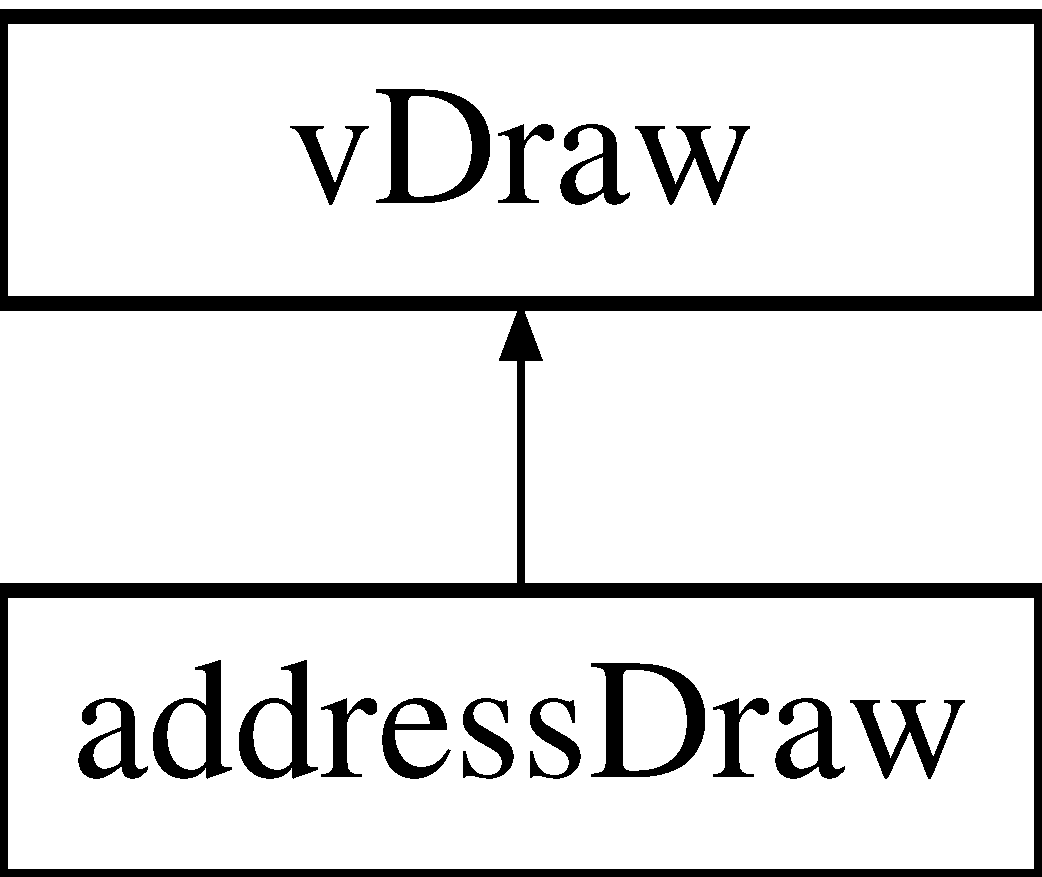
\includegraphics[height=2.000000cm]{classaddressDraw}
\end{center}
\end{figure}
\subsection*{Public Member Functions}
\begin{DoxyCompactItemize}
\item 
virtual void \hyperlink{classaddressDraw_a2eb36efe557d39dfcc49bd5250ec3d6b}{draw} (cv\+::\+Mat \&image, const ev\+::v\+Queue \&e\+Set, int v\+Time)
\begin{DoxyCompactList}\small\item\em draw takes an image and overlays the new visualisation textures \end{DoxyCompactList}\item 
virtual std\+::string \hyperlink{classaddressDraw_a1b1ef76932c71300e87353cc266eb322}{get\+Draw\+Type} ()
\begin{DoxyCompactList}\small\item\em get\+Tag returns the unique code for this drawing method. The arguments given on the command line must match this code exactly \end{DoxyCompactList}\item 
virtual std\+::string {\bfseries get\+Event\+Type} ()\hypertarget{classaddressDraw_a58dc1feb45fb9374b8e89bfb722019cd}{}\label{classaddressDraw_a58dc1feb45fb9374b8e89bfb722019cd}

\end{DoxyCompactItemize}
\subsection*{Static Public Attributes}
\begin{DoxyCompactItemize}
\item 
static const std\+::string {\bfseries drawtype} = \char`\"{}AE\char`\"{}\hypertarget{classaddressDraw_a328ccdbe446c69685affbf11eaac806f}{}\label{classaddressDraw_a328ccdbe446c69685affbf11eaac806f}

\end{DoxyCompactItemize}
\subsection*{Additional Inherited Members}


\subsection{Member Function Documentation}
\index{address\+Draw@{address\+Draw}!draw@{draw}}
\index{draw@{draw}!address\+Draw@{address\+Draw}}
\subsubsection[{\texorpdfstring{draw(cv\+::\+Mat \&image, const ev\+::v\+Queue \&e\+Set, int v\+Time)}{draw(cv::Mat &image, const ev::vQueue &eSet, int vTime)}}]{\setlength{\rightskip}{0pt plus 5cm}void address\+Draw\+::draw (
\begin{DoxyParamCaption}
\item[{cv\+::\+Mat \&}]{canvas, }
\item[{const ev\+::v\+Queue \&}]{e\+Set, }
\item[{int}]{v\+Time}
\end{DoxyParamCaption}
)\hspace{0.3cm}{\ttfamily [virtual]}}\hypertarget{classaddressDraw_a2eb36efe557d39dfcc49bd5250ec3d6b}{}\label{classaddressDraw_a2eb36efe557d39dfcc49bd5250ec3d6b}


draw takes an image and overlays the new visualisation textures 


\begin{DoxyParams}{Parameters}
{\em canvas} & is the image which may or may not yet exist \\
\hline
{\em e\+Set} & is the set of events which could possibly be drawn \\
\hline
\end{DoxyParams}


Implements \hyperlink{classvDraw_a35cf7b42fe542fd51c1014de19fb114c}{v\+Draw}.

\index{address\+Draw@{address\+Draw}!get\+Draw\+Type@{get\+Draw\+Type}}
\index{get\+Draw\+Type@{get\+Draw\+Type}!address\+Draw@{address\+Draw}}
\subsubsection[{\texorpdfstring{get\+Draw\+Type()}{getDrawType()}}]{\setlength{\rightskip}{0pt plus 5cm}std\+::string address\+Draw\+::get\+Draw\+Type (
\begin{DoxyParamCaption}
{}
\end{DoxyParamCaption}
)\hspace{0.3cm}{\ttfamily [virtual]}}\hypertarget{classaddressDraw_a1b1ef76932c71300e87353cc266eb322}{}\label{classaddressDraw_a1b1ef76932c71300e87353cc266eb322}


get\+Tag returns the unique code for this drawing method. The arguments given on the command line must match this code exactly 

\begin{DoxyReturn}{Returns}
the tag code 
\end{DoxyReturn}


Implements \hyperlink{classvDraw_abb4aa2bb3bb8daca40bdb12cd55d3fd3}{v\+Draw}.



The documentation for this class was generated from the following files\+:\begin{DoxyCompactItemize}
\item 
/home/aglover/workspace/projects/event-\/driven/src/processing/v\+Framer/include/v\+Draw.\+h\item 
/home/aglover/workspace/projects/event-\/driven/src/processing/v\+Framer/src/v\+Draw.\+cpp\end{DoxyCompactItemize}

\hypertarget{classev_1_1AddressEvent}{}\section{ev\+:\+:Address\+Event Class Reference}
\label{classev_1_1AddressEvent}\index{ev\+::\+Address\+Event@{ev\+::\+Address\+Event}}


an event with a pixel location, camera number and polarity  




{\ttfamily \#include $<$v\+Codec.\+h$>$}

Inheritance diagram for ev\+:\+:Address\+Event\+:\begin{figure}[H]
\begin{center}
\leavevmode
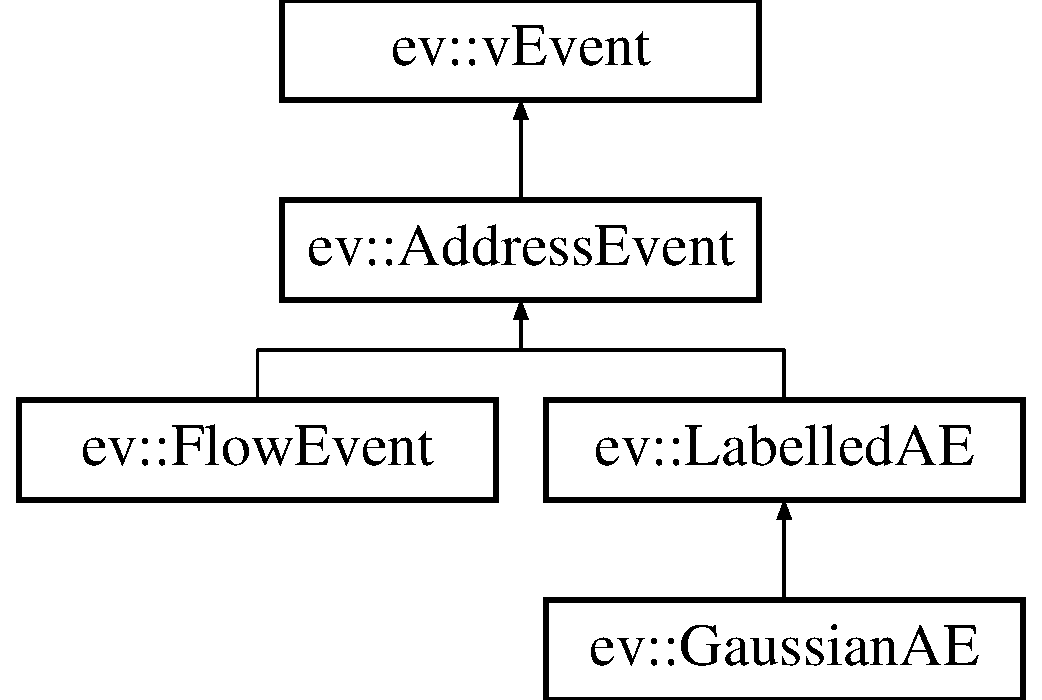
\includegraphics[height=4.000000cm]{classev_1_1AddressEvent}
\end{center}
\end{figure}
\subsection*{Public Member Functions}
\begin{DoxyCompactItemize}
\item 
{\bfseries Address\+Event} (const \hyperlink{classev_1_1vEvent}{v\+Event} \&v)\hypertarget{classev_1_1AddressEvent_a62e810ce50e155828957e61c99a165d2}{}\label{classev_1_1AddressEvent_a62e810ce50e155828957e61c99a165d2}

\item 
{\bfseries Address\+Event} (const \hyperlink{classev_1_1AddressEvent}{Address\+Event} \&v)\hypertarget{classev_1_1AddressEvent_a5072b43ca93fdcdf0294ecff78f3b424}{}\label{classev_1_1AddressEvent_a5072b43ca93fdcdf0294ecff78f3b424}

\item 
virtual event {\bfseries clone} ()\hypertarget{classev_1_1AddressEvent_adabe75246de88f722d65b4994c7955eb}{}\label{classev_1_1AddressEvent_adabe75246de88f722d65b4994c7955eb}

\item 
virtual void {\bfseries encode} (yarp\+::os\+::\+Bottle \&b) const \hypertarget{classev_1_1AddressEvent_a38b726cef241624c31312a3eb1f46730}{}\label{classev_1_1AddressEvent_a38b726cef241624c31312a3eb1f46730}

\item 
virtual bool {\bfseries decode} (const yarp\+::os\+::\+Bottle \&packet, int \&pos)\hypertarget{classev_1_1AddressEvent_a91d805c2aeb136bb23e4da04e29d98b1}{}\label{classev_1_1AddressEvent_a91d805c2aeb136bb23e4da04e29d98b1}

\item 
virtual yarp\+::os\+::\+Property {\bfseries get\+Content} () const \hypertarget{classev_1_1AddressEvent_ad235efba4a6bd3fc79b853ecefad88c9}{}\label{classev_1_1AddressEvent_ad235efba4a6bd3fc79b853ecefad88c9}

\item 
virtual std\+::string {\bfseries get\+Type} () const \hypertarget{classev_1_1AddressEvent_aef0dd1b9a82c2745ccaa0cfc9105df55}{}\label{classev_1_1AddressEvent_aef0dd1b9a82c2745ccaa0cfc9105df55}

\item 
virtual int {\bfseries get\+Channel} () const \hypertarget{classev_1_1AddressEvent_a88038634ab480b42ac1f056abe004b5d}{}\label{classev_1_1AddressEvent_a88038634ab480b42ac1f056abe004b5d}

\item 
virtual void {\bfseries set\+Channel} (const int channel)\hypertarget{classev_1_1AddressEvent_a50e188b1c5702cab67a2175b81c32767}{}\label{classev_1_1AddressEvent_a50e188b1c5702cab67a2175b81c32767}

\end{DoxyCompactItemize}
\subsection*{Public Attributes}
\begin{DoxyCompactItemize}
\item 
unsigned int {\bfseries x}\+:10\hypertarget{classev_1_1AddressEvent_ab6015dc7a789cb6ff7546c47d58829bf}{}\label{classev_1_1AddressEvent_ab6015dc7a789cb6ff7546c47d58829bf}

\item 
unsigned int {\bfseries y}\+:10\hypertarget{classev_1_1AddressEvent_a2e6918d9a0c935c2424e8096ed610c6f}{}\label{classev_1_1AddressEvent_a2e6918d9a0c935c2424e8096ed610c6f}

\item 
unsigned int {\bfseries channel}\+:1\hypertarget{classev_1_1AddressEvent_ab96b9ac3a42cf1d69859f1edbea9cc7f}{}\label{classev_1_1AddressEvent_ab96b9ac3a42cf1d69859f1edbea9cc7f}

\item 
unsigned int {\bfseries polarity}\+:1\hypertarget{classev_1_1AddressEvent_a79bbcea834183012aa39e9d4b2c594ed}{}\label{classev_1_1AddressEvent_a79bbcea834183012aa39e9d4b2c594ed}

\end{DoxyCompactItemize}
\subsection*{Static Public Attributes}
\begin{DoxyCompactItemize}
\item 
static const std\+::string {\bfseries tag} = \char`\"{}AE\char`\"{}\hypertarget{classev_1_1AddressEvent_a9a2d3e863964a1247ae4203a4ad2c646}{}\label{classev_1_1AddressEvent_a9a2d3e863964a1247ae4203a4ad2c646}

\end{DoxyCompactItemize}


\subsection{Detailed Description}
an event with a pixel location, camera number and polarity 

The documentation for this class was generated from the following files\+:\begin{DoxyCompactItemize}
\item 
/home/aglover/workspace/projects/event-\/driven/libraries/include/i\+Cub/eventdriven/v\+Codec.\+h\item 
/home/aglover/workspace/projects/event-\/driven/libraries/src/codecs/codec\+\_\+\+Address\+Event.\+cpp\end{DoxyCompactItemize}

\hypertarget{classAutoSaccadeModule}{}\section{Auto\+Saccade\+Module Class Reference}
\label{classAutoSaccadeModule}\index{Auto\+Saccade\+Module@{Auto\+Saccade\+Module}}
Inheritance diagram for Auto\+Saccade\+Module\+:\begin{figure}[H]
\begin{center}
\leavevmode
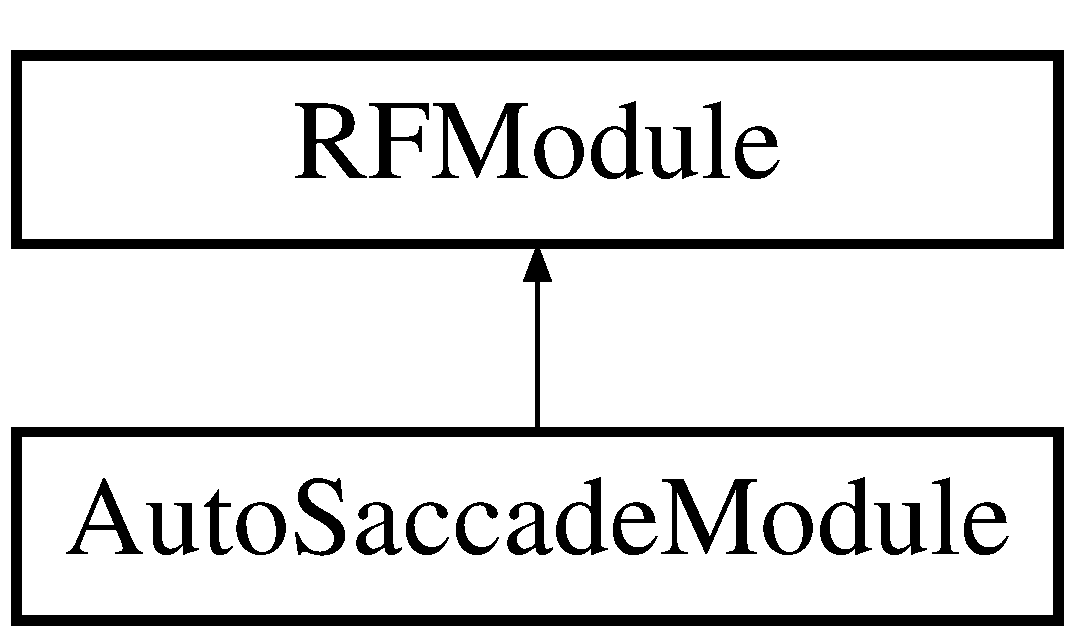
\includegraphics[height=2.000000cm]{classAutoSaccadeModule}
\end{center}
\end{figure}
\subsection*{Public Member Functions}
\begin{DoxyCompactItemize}
\item 
virtual bool {\bfseries configure} (yarp\+::os\+::\+Resource\+Finder \&rf)\hypertarget{classAutoSaccadeModule_a1a912da87f48512567024079a5db2676}{}\label{classAutoSaccadeModule_a1a912da87f48512567024079a5db2676}

\item 
virtual bool {\bfseries interrupt\+Module} ()\hypertarget{classAutoSaccadeModule_a287fec90d0e45f6f0b51b7f0dac33380}{}\label{classAutoSaccadeModule_a287fec90d0e45f6f0b51b7f0dac33380}

\item 
virtual bool {\bfseries close} ()\hypertarget{classAutoSaccadeModule_a93e88144dd31b671adb6a68ec3fd30b3}{}\label{classAutoSaccadeModule_a93e88144dd31b671adb6a68ec3fd30b3}

\item 
virtual bool {\bfseries respond} (const yarp\+::os\+::\+Bottle \&command, yarp\+::os\+::\+Bottle \&reply)\hypertarget{classAutoSaccadeModule_ac55e366df0b53aed2aa872fb171b439f}{}\label{classAutoSaccadeModule_ac55e366df0b53aed2aa872fb171b439f}

\item 
virtual double {\bfseries get\+Period} ()\hypertarget{classAutoSaccadeModule_a389e0a4d1e17fc5d669bc499854ca6e3}{}\label{classAutoSaccadeModule_a389e0a4d1e17fc5d669bc499854ca6e3}

\item 
virtual bool {\bfseries update\+Module} ()\hypertarget{classAutoSaccadeModule_a5812e03b212a3fbc960990ce699ae6b7}{}\label{classAutoSaccadeModule_a5812e03b212a3fbc960990ce699ae6b7}

\end{DoxyCompactItemize}


The documentation for this class was generated from the following files\+:\begin{DoxyCompactItemize}
\item 
/home/aglover/workspace/projects/event-\/driven/src/applications/autosaccade/include/auto\+Saccade.\+h\item 
/home/aglover/workspace/projects/event-\/driven/src/applications/autosaccade/src/auto\+Saccade.\+cpp\end{DoxyCompactItemize}

\hypertarget{classblobDraw}{}\section{blob\+Draw Class Reference}
\label{classblobDraw}\index{blob\+Draw@{blob\+Draw}}
Inheritance diagram for blob\+Draw\+:\begin{figure}[H]
\begin{center}
\leavevmode
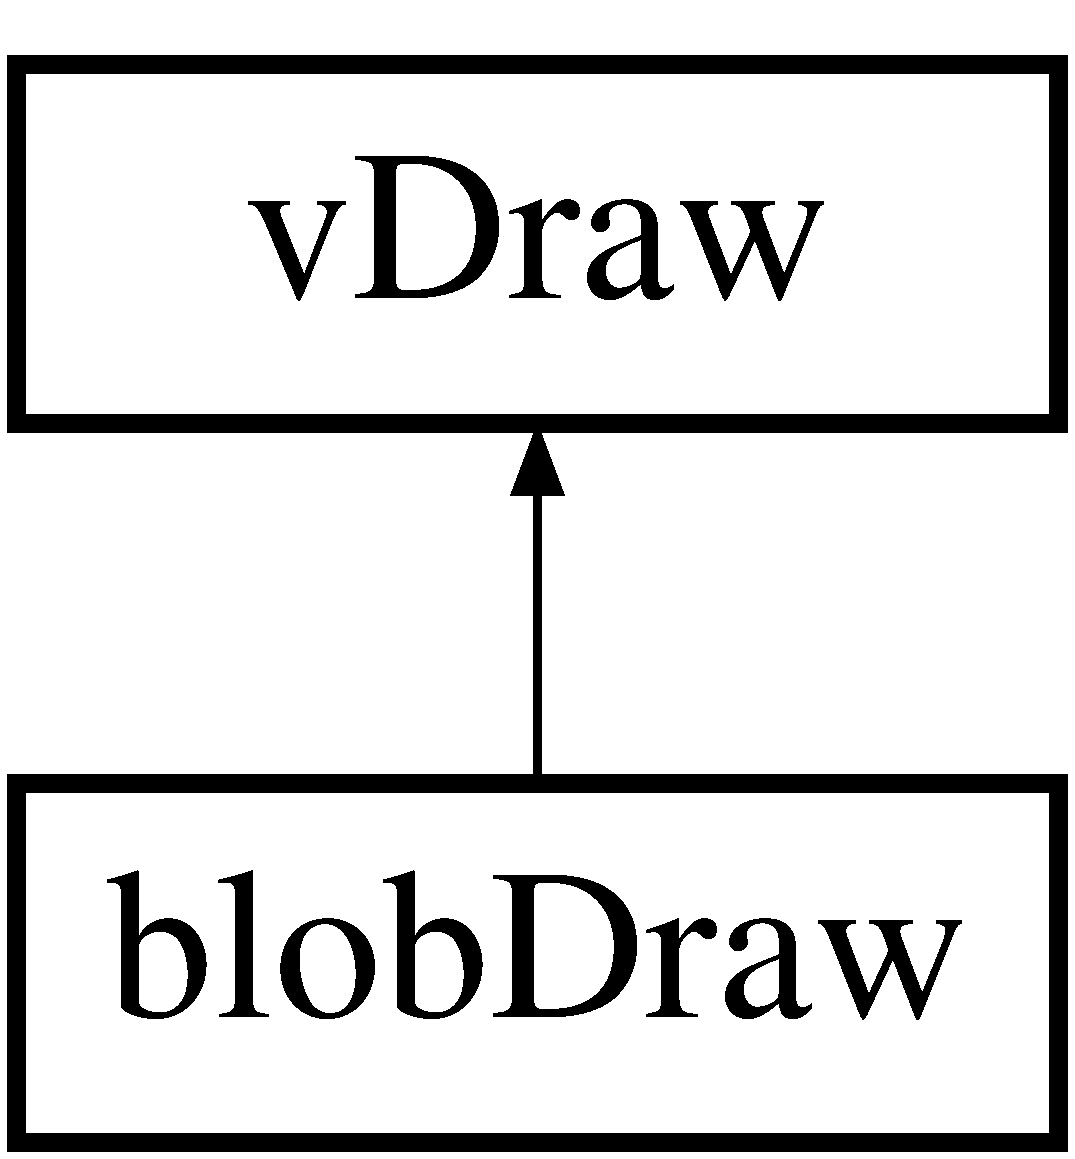
\includegraphics[height=2.000000cm]{classblobDraw}
\end{center}
\end{figure}
\subsection*{Public Member Functions}
\begin{DoxyCompactItemize}
\item 
virtual void \hyperlink{classblobDraw_ae29fcd93142586e3f3ab070f795f26fe}{draw} (cv\+::\+Mat \&image, const ev\+::v\+Queue \&e\+Set, int v\+Time)
\begin{DoxyCompactList}\small\item\em draw takes an image and overlays the new visualisation textures \end{DoxyCompactList}\item 
virtual std\+::string \hyperlink{classblobDraw_a72b6e196fcd44371a4cdfa734d19dc93}{get\+Draw\+Type} ()
\begin{DoxyCompactList}\small\item\em get\+Tag returns the unique code for this drawing method. The arguments given on the command line must match this code exactly \end{DoxyCompactList}\item 
virtual std\+::string {\bfseries get\+Event\+Type} ()\hypertarget{classblobDraw_a9edd0c705b8a24070d3e7ce84e4c9bde}{}\label{classblobDraw_a9edd0c705b8a24070d3e7ce84e4c9bde}

\end{DoxyCompactItemize}
\subsection*{Static Public Attributes}
\begin{DoxyCompactItemize}
\item 
static const std\+::string {\bfseries drawtype} = \char`\"{}B\+L\+OB\char`\"{}\hypertarget{classblobDraw_a79d4c5e42927549ee3ff075abaf87eb5}{}\label{classblobDraw_a79d4c5e42927549ee3ff075abaf87eb5}

\end{DoxyCompactItemize}
\subsection*{Additional Inherited Members}


\subsection{Member Function Documentation}
\index{blob\+Draw@{blob\+Draw}!draw@{draw}}
\index{draw@{draw}!blob\+Draw@{blob\+Draw}}
\subsubsection[{\texorpdfstring{draw(cv\+::\+Mat \&image, const ev\+::v\+Queue \&e\+Set, int v\+Time)}{draw(cv::Mat &image, const ev::vQueue &eSet, int vTime)}}]{\setlength{\rightskip}{0pt plus 5cm}void blob\+Draw\+::draw (
\begin{DoxyParamCaption}
\item[{cv\+::\+Mat \&}]{canvas, }
\item[{const ev\+::v\+Queue \&}]{e\+Set, }
\item[{int}]{v\+Time}
\end{DoxyParamCaption}
)\hspace{0.3cm}{\ttfamily [virtual]}}\hypertarget{classblobDraw_ae29fcd93142586e3f3ab070f795f26fe}{}\label{classblobDraw_ae29fcd93142586e3f3ab070f795f26fe}


draw takes an image and overlays the new visualisation textures 


\begin{DoxyParams}{Parameters}
{\em canvas} & is the image which may or may not yet exist \\
\hline
{\em e\+Set} & is the set of events which could possibly be drawn \\
\hline
\end{DoxyParams}


Implements \hyperlink{classvDraw_a35cf7b42fe542fd51c1014de19fb114c}{v\+Draw}.

\index{blob\+Draw@{blob\+Draw}!get\+Draw\+Type@{get\+Draw\+Type}}
\index{get\+Draw\+Type@{get\+Draw\+Type}!blob\+Draw@{blob\+Draw}}
\subsubsection[{\texorpdfstring{get\+Draw\+Type()}{getDrawType()}}]{\setlength{\rightskip}{0pt plus 5cm}std\+::string blob\+Draw\+::get\+Draw\+Type (
\begin{DoxyParamCaption}
{}
\end{DoxyParamCaption}
)\hspace{0.3cm}{\ttfamily [virtual]}}\hypertarget{classblobDraw_a72b6e196fcd44371a4cdfa734d19dc93}{}\label{classblobDraw_a72b6e196fcd44371a4cdfa734d19dc93}


get\+Tag returns the unique code for this drawing method. The arguments given on the command line must match this code exactly 

\begin{DoxyReturn}{Returns}
the tag code 
\end{DoxyReturn}


Implements \hyperlink{classvDraw_abb4aa2bb3bb8daca40bdb12cd55d3fd3}{v\+Draw}.



The documentation for this class was generated from the following files\+:\begin{DoxyCompactItemize}
\item 
/home/aglover/workspace/projects/event-\/driven/src/processing/v\+Framer/include/v\+Draw.\+h\item 
/home/aglover/workspace/projects/event-\/driven/src/processing/v\+Framer/src/v\+Draw.\+cpp\end{DoxyCompactItemize}

\hypertarget{classBlobTracker}{}\section{Blob\+Tracker Class Reference}
\label{classBlobTracker}\index{Blob\+Tracker@{Blob\+Tracker}}
\subsection*{Public Member Functions}
\begin{DoxyCompactItemize}
\item 
bool {\bfseries initialise\+Position} (double x, double y)\hypertarget{classBlobTracker_ac3dbde755642d5e9cf179123823a8eec}{}\label{classBlobTracker_ac3dbde755642d5e9cf179123823a8eec}

\item 
bool {\bfseries initialise\+Shape} (double sigX, double sig\+Y2, double sig\+XY, double alpha\+\_\+pos, double alpha\+\_\+shape, bool fix)\hypertarget{classBlobTracker_a29990e53b163a720f284978b97a6d723}{}\label{classBlobTracker_a29990e53b163a720f284978b97a6d723}

\item 
double {\bfseries dist2event} (int ev\+\_\+x, int ev\+\_\+y)\hypertarget{classBlobTracker_a873c6f0932845537163a5b80605ac599}{}\label{classBlobTracker_a873c6f0932845537163a5b80605ac599}

\item 
double {\bfseries compute\+\_\+p} (int ev\+\_\+x, int ev\+\_\+y)\hypertarget{classBlobTracker_abfe11c1db8b5c9634ec9f5ba86f379d9}{}\label{classBlobTracker_abfe11c1db8b5c9634ec9f5ba86f379d9}

\item 
bool {\bfseries add\+Activity} (int x, int y, unsigned long int ts, double Tact, double Tevent)\hypertarget{classBlobTracker_ab84953899ecee068e63a8f1a89fe7dd8}{}\label{classBlobTracker_ab84953899ecee068e63a8f1a89fe7dd8}

\item 
bool {\bfseries decay\+Activity} (int dt, double tau, double Tinact, double Tfree)\hypertarget{classBlobTracker_af410be534735ad33bafc259d70316a54}{}\label{classBlobTracker_af410be534735ad33bafc259d70316a54}

\item 
void {\bfseries cluster\+Spiked} ()\hypertarget{classBlobTracker_af7a07b561d9516ab480632667672e7ed}{}\label{classBlobTracker_af7a07b561d9516ab480632667672e7ed}

\item 
void {\bfseries is\+No\+Longer\+Free} ()\hypertarget{classBlobTracker_ad22b6a8aaf647e71b57fba25f9f419d1}{}\label{classBlobTracker_ad22b6a8aaf647e71b57fba25f9f419d1}

\item 
bool {\bfseries is\+\_\+active} ()\hypertarget{classBlobTracker_af0cd5a8da431251197c88560c919d89d}{}\label{classBlobTracker_af0cd5a8da431251197c88560c919d89d}

\item 
bool {\bfseries is\+\_\+on} ()\hypertarget{classBlobTracker_a8f18821eb105ce6e95d05e4cc4e3a3aa}{}\label{classBlobTracker_a8f18821eb105ce6e95d05e4cc4e3a3aa}

\item 
bool {\bfseries is\+Free} ()\hypertarget{classBlobTracker_a21f9c5029c220f71e7442a8b068431b7}{}\label{classBlobTracker_a21f9c5029c220f71e7442a8b068431b7}

\item 
double {\bfseries get\+\_\+sigx2} ()\hypertarget{classBlobTracker_ab42f73b98cb1885cdd162148ace8bf23}{}\label{classBlobTracker_ab42f73b98cb1885cdd162148ace8bf23}

\item 
double {\bfseries get\+\_\+sigy2} ()\hypertarget{classBlobTracker_a6cc4fcfc6ade9a856dc7ba502531adf5}{}\label{classBlobTracker_a6cc4fcfc6ade9a856dc7ba502531adf5}

\item 
double {\bfseries get\+\_\+sigxy} ()\hypertarget{classBlobTracker_aeb6aed3ccd9793682b005127fab2bffd}{}\label{classBlobTracker_aeb6aed3ccd9793682b005127fab2bffd}

\item 
int {\bfseries get\+\_\+x} ()\hypertarget{classBlobTracker_aa20dbabdbbfabb44301d18bc59881488}{}\label{classBlobTracker_aa20dbabdbbfabb44301d18bc59881488}

\item 
int {\bfseries get\+\_\+y} ()\hypertarget{classBlobTracker_a2d78cea632f8f9fa4b325c575b9b49d9}{}\label{classBlobTracker_a2d78cea632f8f9fa4b325c575b9b49d9}

\item 
double {\bfseries get\+\_\+vx} ()\hypertarget{classBlobTracker_a339a2cdbf0e3af39241abc7dac115f6c}{}\label{classBlobTracker_a339a2cdbf0e3af39241abc7dac115f6c}

\item 
double {\bfseries get\+\_\+vy} ()\hypertarget{classBlobTracker_a99050a07f515b524837a3977e9c53a9c}{}\label{classBlobTracker_a99050a07f515b524837a3977e9c53a9c}

\item 
double {\bfseries get\+\_\+act} ()\hypertarget{classBlobTracker_a8b59d7b66e32c3c55486f7ef7446fbde}{}\label{classBlobTracker_a8b59d7b66e32c3c55486f7ef7446fbde}

\end{DoxyCompactItemize}
\subsection*{Protected Types}
\begin{DoxyCompactItemize}
\item 
enum {\bfseries State} \{ {\bfseries Active}, 
{\bfseries Inactive}, 
{\bfseries Free}
 \}\hypertarget{classBlobTracker_a7e8d5dcd8736e3ae2a1c448a36e3516f}{}\label{classBlobTracker_a7e8d5dcd8736e3ae2a1c448a36e3516f}

\end{DoxyCompactItemize}
\subsection*{Protected Attributes}
\begin{DoxyCompactItemize}
\item 
State {\bfseries state\+\_\+}\hypertarget{classBlobTracker_ad96c96edcf8e9b2155aba3c39d128249}{}\label{classBlobTracker_ad96c96edcf8e9b2155aba3c39d128249}

\item 
double {\bfseries cen\+\_\+x\+\_\+}\hypertarget{classBlobTracker_a93b360b9499b9a77c7da2eb0b264d8af}{}\label{classBlobTracker_a93b360b9499b9a77c7da2eb0b264d8af}

\item 
double {\bfseries cen\+\_\+y\+\_\+}\hypertarget{classBlobTracker_ab5eaa89cfedfb25fc0881009cefdbea4}{}\label{classBlobTracker_ab5eaa89cfedfb25fc0881009cefdbea4}

\item 
double {\bfseries sig\+\_\+x2\+\_\+}\hypertarget{classBlobTracker_a90039cb4599ff8cf137d0b0a9b89801e}{}\label{classBlobTracker_a90039cb4599ff8cf137d0b0a9b89801e}

\item 
double {\bfseries sig\+\_\+y2\+\_\+}\hypertarget{classBlobTracker_a8fa7fa36db3faed93d94b30bd50449e1}{}\label{classBlobTracker_a8fa7fa36db3faed93d94b30bd50449e1}

\item 
double {\bfseries sig\+\_\+xy\+\_\+}\hypertarget{classBlobTracker_af7c64be12d9aeee877adc6027e57dc31}{}\label{classBlobTracker_af7c64be12d9aeee877adc6027e57dc31}

\item 
double {\bfseries v\+LastX}\hypertarget{classBlobTracker_a37789b44e5e478a237580a3e168bd496}{}\label{classBlobTracker_a37789b44e5e478a237580a3e168bd496}

\item 
double {\bfseries v\+LastY}\hypertarget{classBlobTracker_ae836b9dd8d830ba8f6ccb6ea2f80e313}{}\label{classBlobTracker_ae836b9dd8d830ba8f6ccb6ea2f80e313}

\item 
double {\bfseries vx\+\_\+}\hypertarget{classBlobTracker_a98a091e1f3a0e16a71ff6602079c9c23}{}\label{classBlobTracker_a98a091e1f3a0e16a71ff6602079c9c23}

\item 
double {\bfseries vy\+\_\+}\hypertarget{classBlobTracker_a5b41c1c66d14c8b794b314ba204a93bd}{}\label{classBlobTracker_a5b41c1c66d14c8b794b314ba204a93bd}

\item 
double {\bfseries alpha\+\_\+pos\+\_\+}\hypertarget{classBlobTracker_ae10a65c546bfa9ed53d341a46080f53f}{}\label{classBlobTracker_ae10a65c546bfa9ed53d341a46080f53f}

\item 
double {\bfseries alpha\+\_\+shape\+\_\+}\hypertarget{classBlobTracker_a5183d2c99bd9dbc6f7170050e5830dea}{}\label{classBlobTracker_a5183d2c99bd9dbc6f7170050e5830dea}

\item 
bool {\bfseries fixed\+\_\+shape\+\_\+}\hypertarget{classBlobTracker_a57841b67cf49324e2ff7b9698897e908}{}\label{classBlobTracker_a57841b67cf49324e2ff7b9698897e908}

\item 
double {\bfseries activity\+\_\+}\hypertarget{classBlobTracker_aaf83587414449f41fa7719f9939c48a8}{}\label{classBlobTracker_aaf83587414449f41fa7719f9939c48a8}

\item 
unsigned long int {\bfseries ts\+\_\+last\+\_\+update\+\_\+}\hypertarget{classBlobTracker_a4084fae015313204286ce98259856467}{}\label{classBlobTracker_a4084fae015313204286ce98259856467}

\end{DoxyCompactItemize}


The documentation for this class was generated from the following files\+:\begin{DoxyCompactItemize}
\item 
/home/aglover/workspace/projects/event-\/driven/src/processing/v\+Cluster/include/blob\+Tracker.\+h\item 
/home/aglover/workspace/projects/event-\/driven/src/processing/v\+Cluster/src/blob\+Tracker.\+cpp\end{DoxyCompactItemize}

\hypertarget{classclusterDraw}{}\section{cluster\+Draw Class Reference}
\label{classclusterDraw}\index{cluster\+Draw@{cluster\+Draw}}
Inheritance diagram for cluster\+Draw\+:\begin{figure}[H]
\begin{center}
\leavevmode
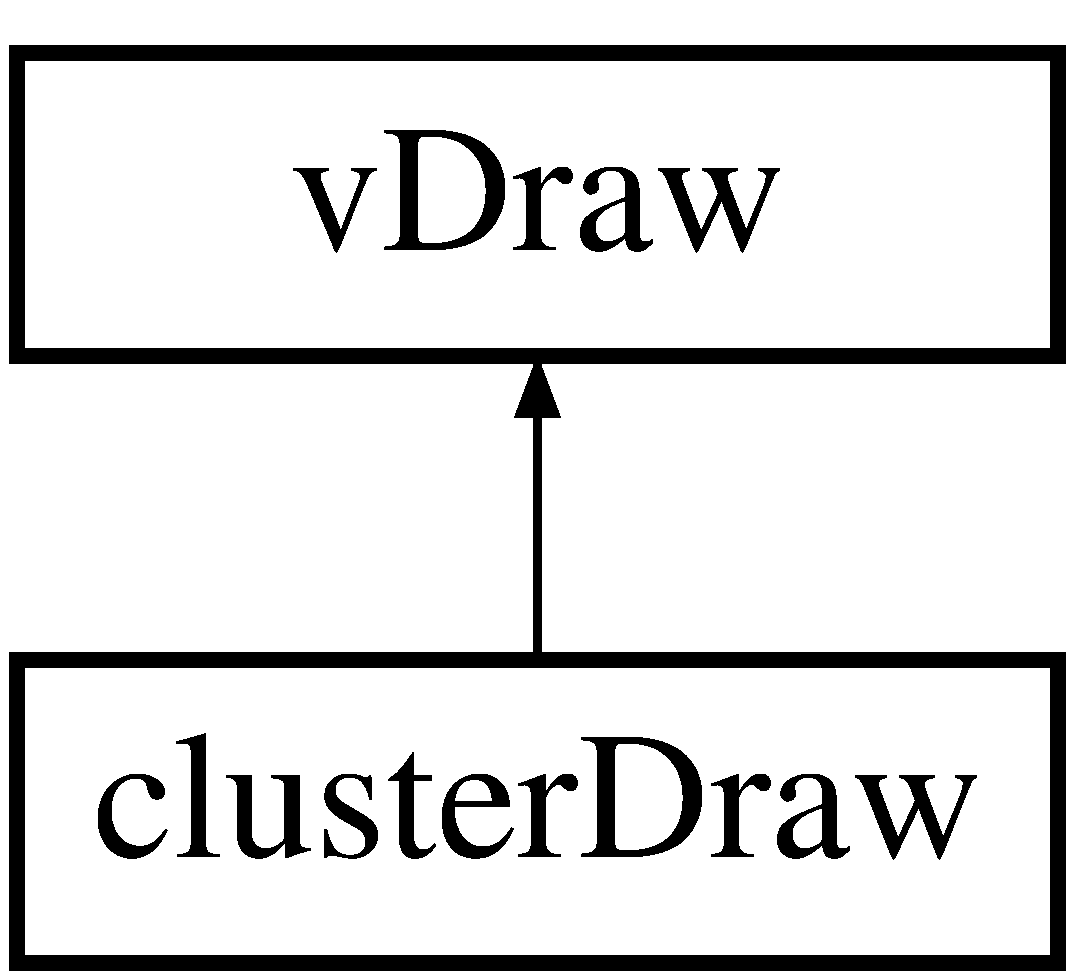
\includegraphics[height=2.000000cm]{classclusterDraw}
\end{center}
\end{figure}
\subsection*{Public Member Functions}
\begin{DoxyCompactItemize}
\item 
virtual void \hyperlink{classclusterDraw_a4e76b182dc58c06d701e7d44a66de79c}{draw} (cv\+::\+Mat \&image, const ev\+::v\+Queue \&e\+Set, int v\+Time)
\begin{DoxyCompactList}\small\item\em draw takes an image and overlays the new visualisation textures \end{DoxyCompactList}\item 
virtual std\+::string \hyperlink{classclusterDraw_a1195b2532670913822405dbd8193e0d4}{get\+Draw\+Type} ()
\begin{DoxyCompactList}\small\item\em get\+Tag returns the unique code for this drawing method. The arguments given on the command line must match this code exactly \end{DoxyCompactList}\item 
virtual std\+::string {\bfseries get\+Event\+Type} ()\hypertarget{classclusterDraw_acec9468f4143e1efc323fa2da9958784}{}\label{classclusterDraw_acec9468f4143e1efc323fa2da9958784}

\end{DoxyCompactItemize}
\subsection*{Static Public Attributes}
\begin{DoxyCompactItemize}
\item 
static const std\+::string {\bfseries drawtype} = \char`\"{}C\+LE\char`\"{}\hypertarget{classclusterDraw_a3a1b70da319c636064f5f70c5e4e962d}{}\label{classclusterDraw_a3a1b70da319c636064f5f70c5e4e962d}

\end{DoxyCompactItemize}
\subsection*{Protected Attributes}
\begin{DoxyCompactItemize}
\item 
std\+::map$<$ int, ev\+::event$<$ \hyperlink{classev_1_1GaussianAE}{ev\+::\+Gaussian\+AE} $>$ $>$ {\bfseries persistance}\hypertarget{classclusterDraw_ae722227bf0c7b5f675c15a7598e86f79}{}\label{classclusterDraw_ae722227bf0c7b5f675c15a7598e86f79}

\item 
int {\bfseries stagnant\+Count}\hypertarget{classclusterDraw_ad200768ffa7b9659e770a4b8551bc160}{}\label{classclusterDraw_ad200768ffa7b9659e770a4b8551bc160}

\end{DoxyCompactItemize}
\subsection*{Additional Inherited Members}


\subsection{Member Function Documentation}
\index{cluster\+Draw@{cluster\+Draw}!draw@{draw}}
\index{draw@{draw}!cluster\+Draw@{cluster\+Draw}}
\subsubsection[{\texorpdfstring{draw(cv\+::\+Mat \&image, const ev\+::v\+Queue \&e\+Set, int v\+Time)}{draw(cv::Mat &image, const ev::vQueue &eSet, int vTime)}}]{\setlength{\rightskip}{0pt plus 5cm}void cluster\+Draw\+::draw (
\begin{DoxyParamCaption}
\item[{cv\+::\+Mat \&}]{canvas, }
\item[{const ev\+::v\+Queue \&}]{e\+Set, }
\item[{int}]{v\+Time}
\end{DoxyParamCaption}
)\hspace{0.3cm}{\ttfamily [virtual]}}\hypertarget{classclusterDraw_a4e76b182dc58c06d701e7d44a66de79c}{}\label{classclusterDraw_a4e76b182dc58c06d701e7d44a66de79c}


draw takes an image and overlays the new visualisation textures 


\begin{DoxyParams}{Parameters}
{\em canvas} & is the image which may or may not yet exist \\
\hline
{\em e\+Set} & is the set of events which could possibly be drawn \\
\hline
\end{DoxyParams}


Implements \hyperlink{classvDraw_a35cf7b42fe542fd51c1014de19fb114c}{v\+Draw}.

\index{cluster\+Draw@{cluster\+Draw}!get\+Draw\+Type@{get\+Draw\+Type}}
\index{get\+Draw\+Type@{get\+Draw\+Type}!cluster\+Draw@{cluster\+Draw}}
\subsubsection[{\texorpdfstring{get\+Draw\+Type()}{getDrawType()}}]{\setlength{\rightskip}{0pt plus 5cm}std\+::string cluster\+Draw\+::get\+Draw\+Type (
\begin{DoxyParamCaption}
{}
\end{DoxyParamCaption}
)\hspace{0.3cm}{\ttfamily [virtual]}}\hypertarget{classclusterDraw_a1195b2532670913822405dbd8193e0d4}{}\label{classclusterDraw_a1195b2532670913822405dbd8193e0d4}


get\+Tag returns the unique code for this drawing method. The arguments given on the command line must match this code exactly 

\begin{DoxyReturn}{Returns}
the tag code 
\end{DoxyReturn}


Implements \hyperlink{classvDraw_abb4aa2bb3bb8daca40bdb12cd55d3fd3}{v\+Draw}.



The documentation for this class was generated from the following files\+:\begin{DoxyCompactItemize}
\item 
/home/aglover/workspace/projects/event-\/driven/src/processing/v\+Framer/include/v\+Draw.\+h\item 
/home/aglover/workspace/projects/event-\/driven/src/processing/v\+Framer/src/v\+Draw.\+cpp\end{DoxyCompactItemize}

\hypertarget{classev_1_1collectorPort}{}\section{ev\+:\+:collector\+Port Class Reference}
\label{classev_1_1collectorPort}\index{ev\+::collector\+Port@{ev\+::collector\+Port}}


an output port that can safely accept events from multiple threads and sends them at a fixed output rate.  




{\ttfamily \#include $<$v\+Collect\+Send.\+h$>$}

Inheritance diagram for ev\+:\+:collector\+Port\+:\begin{figure}[H]
\begin{center}
\leavevmode
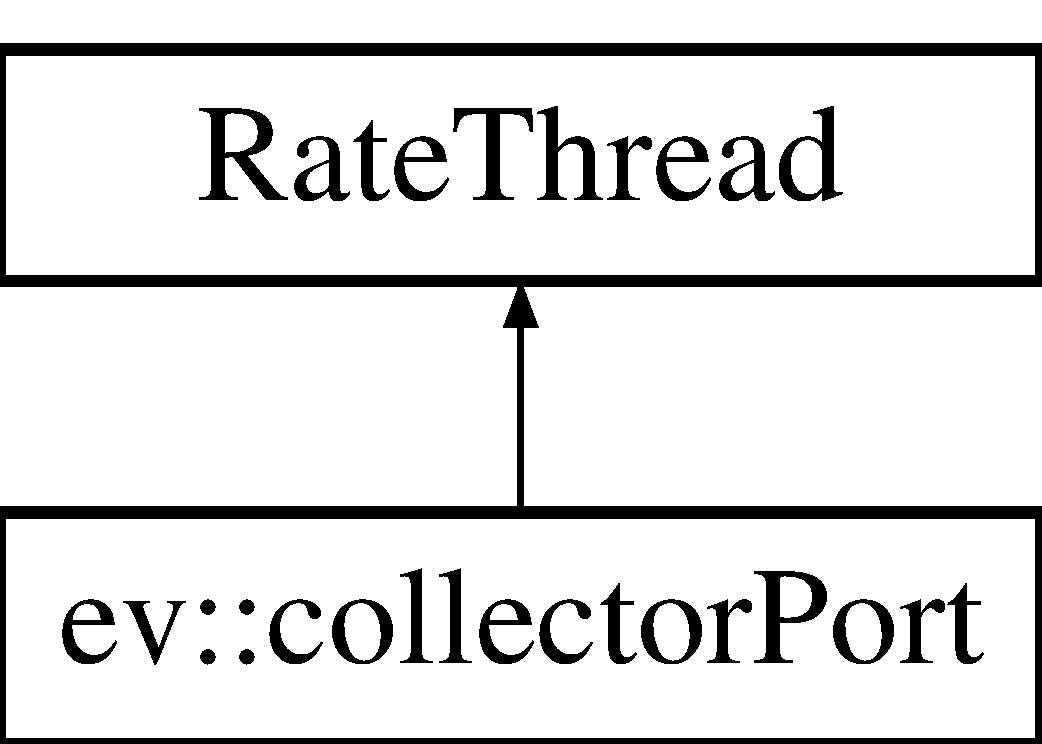
\includegraphics[height=2.000000cm]{classev_1_1collectorPort}
\end{center}
\end{figure}
\subsection*{Public Member Functions}
\begin{DoxyCompactItemize}
\item 
bool {\bfseries open} (std\+::string name)\hypertarget{classev_1_1collectorPort_a164072ae38c4e115873c451984b8e7f4}{}\label{classev_1_1collectorPort_a164072ae38c4e115873c451984b8e7f4}

\item 
void {\bfseries pushevent} (event$<$$>$ v, yarp\+::os\+::\+Stamp y)\hypertarget{classev_1_1collectorPort_ab1d587f6b728b65b22df73bbe674607d}{}\label{classev_1_1collectorPort_ab1d587f6b728b65b22df73bbe674607d}

\item 
void {\bfseries run} ()\hypertarget{classev_1_1collectorPort_a7ec227ae78ec71ca8867a20ae815ea7d}{}\label{classev_1_1collectorPort_a7ec227ae78ec71ca8867a20ae815ea7d}

\end{DoxyCompactItemize}


\subsection{Detailed Description}
an output port that can safely accept events from multiple threads and sends them at a fixed output rate. 

The documentation for this class was generated from the following file\+:\begin{DoxyCompactItemize}
\item 
/home/aglover/workspace/projects/event-\/driven/libraries/include/i\+Cub/eventdriven/v\+Collect\+Send.\+h\end{DoxyCompactItemize}

\hypertarget{classdepthgt}{}\section{depthgt Class Reference}
\label{classdepthgt}\index{depthgt@{depthgt}}
Inheritance diagram for depthgt\+:\begin{figure}[H]
\begin{center}
\leavevmode
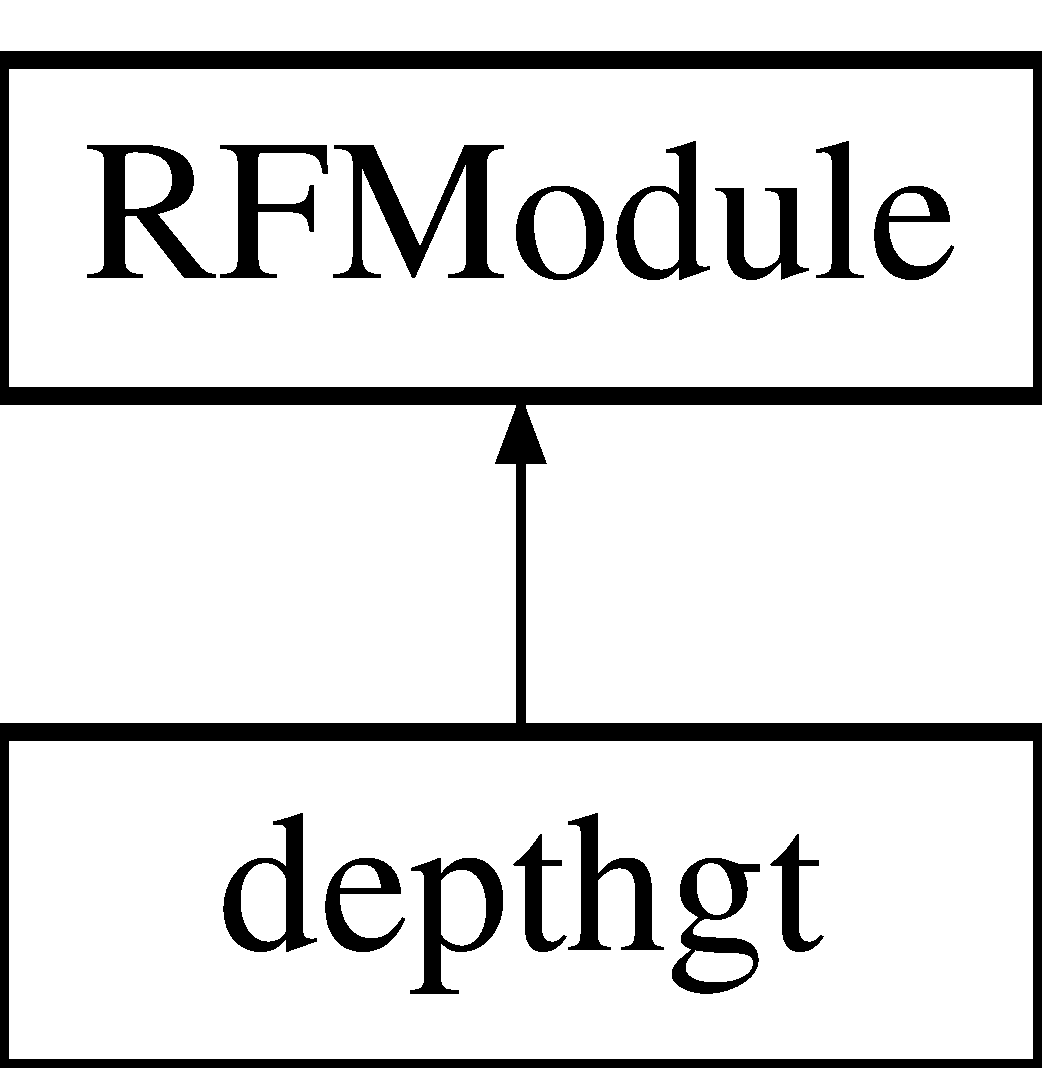
\includegraphics[height=2.000000cm]{classdepthgt}
\end{center}
\end{figure}
\subsection*{Public Member Functions}
\begin{DoxyCompactItemize}
\item 
virtual bool {\bfseries configure} (yarp\+::os\+::\+Resource\+Finder \&rf)\hypertarget{classdepthgt_a336b0e92729120b58670b48ef1704958}{}\label{classdepthgt_a336b0e92729120b58670b48ef1704958}

\item 
virtual bool {\bfseries interrupt\+Module} ()\hypertarget{classdepthgt_a661af7f059e66db284b68a9dd3008b36}{}\label{classdepthgt_a661af7f059e66db284b68a9dd3008b36}

\item 
virtual bool {\bfseries close} ()\hypertarget{classdepthgt_a00c5ecbadb3e09bb45eb2d5663bf8f1f}{}\label{classdepthgt_a00c5ecbadb3e09bb45eb2d5663bf8f1f}

\item 
virtual bool {\bfseries update\+Module} ()\hypertarget{classdepthgt_acb37ecb3e34c1f47dd6c6cb3c167afdb}{}\label{classdepthgt_acb37ecb3e34c1f47dd6c6cb3c167afdb}

\item 
virtual double {\bfseries get\+Period} ()\hypertarget{classdepthgt_ab49d8668b437e2d89e2462625f009962}{}\label{classdepthgt_ab49d8668b437e2d89e2462625f009962}

\end{DoxyCompactItemize}


The documentation for this class was generated from the following files\+:\begin{DoxyCompactItemize}
\item 
/home/aglover/workspace/projects/event-\/driven/src/applications/vergence\+Demo/depth\+G\+T/include/depth\+G\+T.\+h\item 
/home/aglover/workspace/projects/event-\/driven/src/applications/vergence\+Demo/depth\+G\+T/src/depth\+G\+T.\+cpp\end{DoxyCompactItemize}

\hypertarget{classdevice2yarp}{}\section{device2yarp Class Reference}
\label{classdevice2yarp}\index{device2yarp@{device2yarp}}
Inheritance diagram for device2yarp\+:\begin{figure}[H]
\begin{center}
\leavevmode
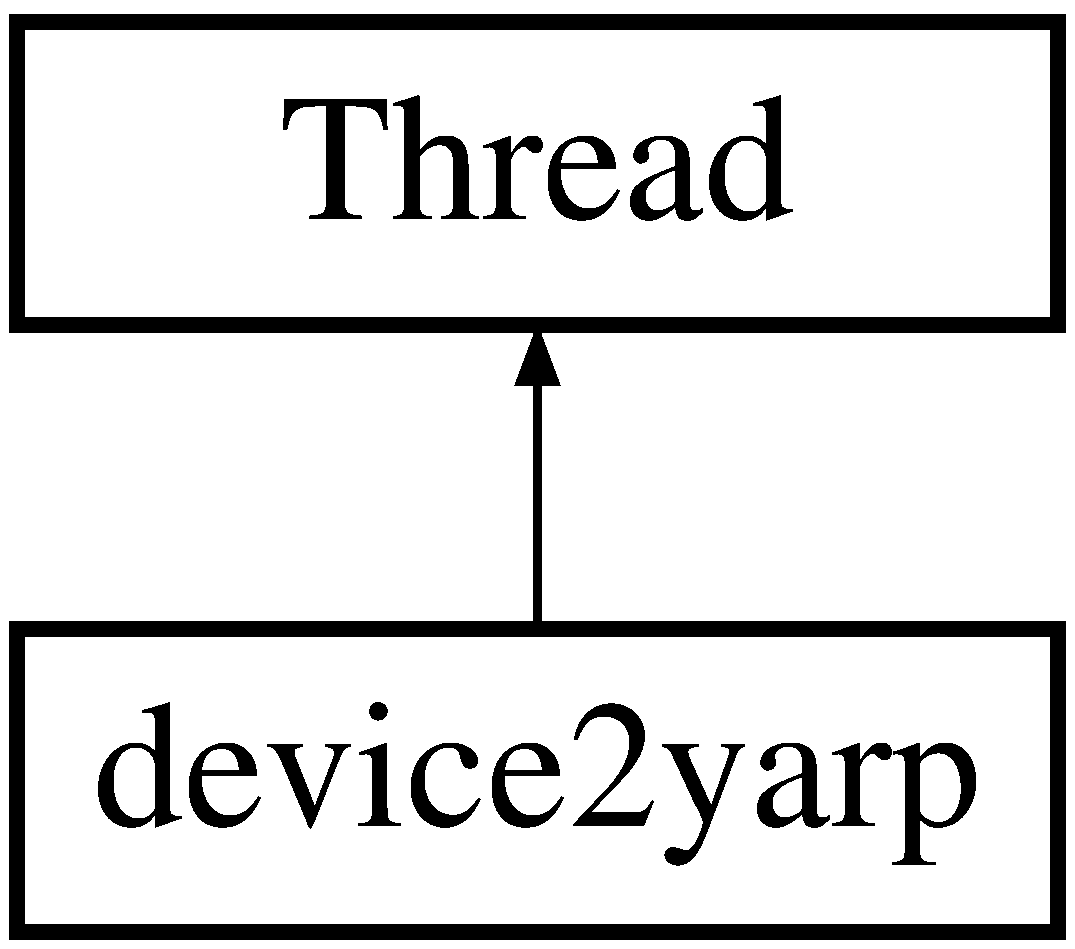
\includegraphics[height=2.000000cm]{classdevice2yarp}
\end{center}
\end{figure}
\subsection*{Public Member Functions}
\begin{DoxyCompactItemize}
\item 
bool {\bfseries initialise} (std\+::string module\+Name=\char`\"{}\char`\"{}, bool strict=false, bool check=false, std\+::string device\+Name=\char`\"{}\char`\"{}, unsigned int buffer\+Size=800000, unsigned int read\+Size=1024)\hypertarget{classdevice2yarp_ab94cdfb71b80d35005b43d42276266e1}{}\label{classdevice2yarp_ab94cdfb71b80d35005b43d42276266e1}

\item 
void {\bfseries initialise\+Filter} (bool applyfilter, int width, int height, int temporalsize, int spatial\+Size)\hypertarget{classdevice2yarp_ad4edcff27efc43f04cc4cc29ae240746}{}\label{classdevice2yarp_ad4edcff27efc43f04cc4cc29ae240746}

\item 
void {\bfseries check\+For\+T\+S\+Jumps} ()\hypertarget{classdevice2yarp_a8f5015246040644a2bf7fcbf9a305a8a}{}\label{classdevice2yarp_a8f5015246040644a2bf7fcbf9a305a8a}

\item 
virtual void {\bfseries run} ()\hypertarget{classdevice2yarp_aa01eb91fc90a62cb29df3fdc8387cb54}{}\label{classdevice2yarp_aa01eb91fc90a62cb29df3fdc8387cb54}

\item 
virtual void {\bfseries thread\+Release} ()\hypertarget{classdevice2yarp_ae429ee3f9ab68ceea96daf63553e7700}{}\label{classdevice2yarp_ae429ee3f9ab68ceea96daf63553e7700}

\item 
virtual void {\bfseries after\+Start} (bool success)\hypertarget{classdevice2yarp_a1098424f146070180d0681787b771451}{}\label{classdevice2yarp_a1098424f146070180d0681787b771451}

\end{DoxyCompactItemize}


The documentation for this class was generated from the following files\+:\begin{DoxyCompactItemize}
\item 
/home/aglover/workspace/projects/event-\/driven/src/hardwareio/zynq\+Grabber/include/yarp\+Interface.\+h\item 
/home/aglover/workspace/projects/event-\/driven/src/hardwareio/zynq\+Grabber/src/yarp\+Interface.\+cpp\end{DoxyCompactItemize}

\hypertarget{classEventBottleManager}{}\section{Event\+Bottle\+Manager Class Reference}
\label{classEventBottleManager}\index{Event\+Bottle\+Manager@{Event\+Bottle\+Manager}}
Inheritance diagram for Event\+Bottle\+Manager\+:\begin{figure}[H]
\begin{center}
\leavevmode
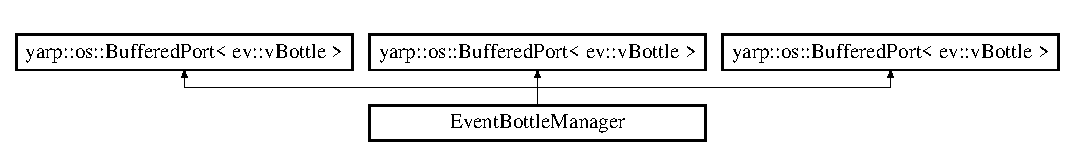
\includegraphics[height=1.659259cm]{classEventBottleManager}
\end{center}
\end{figure}
\subsection*{Public Member Functions}
\begin{DoxyCompactItemize}
\item 
bool {\bfseries open} (const std\+::string \&name)\hypertarget{classEventBottleManager_a41ce7bd0a716ab0a88c1ad505b02d20b}{}\label{classEventBottleManager_a41ce7bd0a716ab0a88c1ad505b02d20b}

\item 
void {\bfseries on\+Read} (\hyperlink{classev_1_1vBottle}{ev\+::v\+Bottle} \&bot)\hypertarget{classEventBottleManager_aa848144d06e1970fb3c0482da838f078}{}\label{classEventBottleManager_aa848144d06e1970fb3c0482da838f078}

\item 
unsigned long int {\bfseries get\+Time} ()\hypertarget{classEventBottleManager_af15b5cfdc457500423111c22dee264d2}{}\label{classEventBottleManager_af15b5cfdc457500423111c22dee264d2}

\item 
unsigned long int {\bfseries pop\+Count} ()\hypertarget{classEventBottleManager_a0b4fd036f14e713194d079467021ba3b}{}\label{classEventBottleManager_a0b4fd036f14e713194d079467021ba3b}

\item 
double {\bfseries get\+Event\+Rate} ()\hypertarget{classEventBottleManager_afff63d519aec2d607661a07d79052377}{}\label{classEventBottleManager_afff63d519aec2d607661a07d79052377}

\item 
ev\+::v\+Queue {\bfseries get\+Events} ()\hypertarget{classEventBottleManager_ae614e9d612bc1994741ff875decd9ee4}{}\label{classEventBottleManager_ae614e9d612bc1994741ff875decd9ee4}

\item 
bool {\bfseries start} ()\hypertarget{classEventBottleManager_ae0f9b17dcf7bbad0c6c79d93b6c7df5e}{}\label{classEventBottleManager_ae0f9b17dcf7bbad0c6c79d93b6c7df5e}

\item 
bool {\bfseries stop} ()\hypertarget{classEventBottleManager_a84ffd3b05e997ab4e92f448459f0da7c}{}\label{classEventBottleManager_a84ffd3b05e997ab4e92f448459f0da7c}

\item 
void {\bfseries set\+All\+Parameters} (double alpha\+\_\+shape, double alpha\+\_\+pos, double Tact, double Tinact, double Tfree, double Tevent, double SigX, double SigY, double Sig\+XY, bool Fixedshape, int Regrate, double Maxdist, double decay\+\_\+tau, double cluster\+Limit)\hypertarget{classEventBottleManager_a451485cebdadbbad730d176894d9f0b1}{}\label{classEventBottleManager_a451485cebdadbbad730d176894d9f0b1}

\item 
bool {\bfseries open} (std\+::string module\+Name)\hypertarget{classEventBottleManager_a82d3237530dcc455f3ceae4e1db4f6df}{}\label{classEventBottleManager_a82d3237530dcc455f3ceae4e1db4f6df}

\item 
bool {\bfseries init} ()\hypertarget{classEventBottleManager_af4d71177a30fdd8fc40485b91abdae10}{}\label{classEventBottleManager_af4d71177a30fdd8fc40485b91abdae10}

\item 
void {\bfseries close} ()\hypertarget{classEventBottleManager_aa155dc6f20728e9f7ff13abf720ea6b8}{}\label{classEventBottleManager_aa155dc6f20728e9f7ff13abf720ea6b8}

\item 
void {\bfseries on\+Read} (\hyperlink{classev_1_1vBottle}{ev\+::v\+Bottle} \&bot)\hypertarget{classEventBottleManager_aa848144d06e1970fb3c0482da838f078}{}\label{classEventBottleManager_aa848144d06e1970fb3c0482da838f078}

\item 
void {\bfseries interrupt} ()\hypertarget{classEventBottleManager_a15152f9daa40714334c2da3871f959a9}{}\label{classEventBottleManager_a15152f9daa40714334c2da3871f959a9}

\item 
void {\bfseries set\+Sensor\+Size} (int sensor\+Height, int sensor\+Width)\hypertarget{classEventBottleManager_a756fda9127e0fc1f8b3781f905f6d28a}{}\label{classEventBottleManager_a756fda9127e0fc1f8b3781f905f6d28a}

\item 
void {\bfseries set\+To\+Truncate} (bool truncate)\hypertarget{classEventBottleManager_a60a4601946a56237640844c40d769fa1}{}\label{classEventBottleManager_a60a4601946a56237640844c40d769fa1}

\item 
void {\bfseries set\+Cam\+Params} (const yarp\+::os\+::\+Bottle \&left, const yarp\+::os\+::\+Bottle \&right)\hypertarget{classEventBottleManager_a1c35cf25905e02c088fbf5de3c24c6e4}{}\label{classEventBottleManager_a1c35cf25905e02c088fbf5de3c24c6e4}

\item 
bool {\bfseries open} (const std\+::string \&name, bool strictio)\hypertarget{classEventBottleManager_ae8cad433fe1b5203bf3a7d03f5ed4639}{}\label{classEventBottleManager_ae8cad433fe1b5203bf3a7d03f5ed4639}

\item 
void {\bfseries close} ()\hypertarget{classEventBottleManager_aa155dc6f20728e9f7ff13abf720ea6b8}{}\label{classEventBottleManager_aa155dc6f20728e9f7ff13abf720ea6b8}

\item 
void {\bfseries interrupt} ()\hypertarget{classEventBottleManager_a15152f9daa40714334c2da3871f959a9}{}\label{classEventBottleManager_a15152f9daa40714334c2da3871f959a9}

\item 
void {\bfseries on\+Read} (\hyperlink{classev_1_1vBottle}{ev\+::v\+Bottle} \&bot)\hypertarget{classEventBottleManager_aa848144d06e1970fb3c0482da838f078}{}\label{classEventBottleManager_aa848144d06e1970fb3c0482da838f078}

\end{DoxyCompactItemize}


The documentation for this class was generated from the following files\+:\begin{DoxyCompactItemize}
\item 
/home/aglover/workspace/projects/event-\/driven/src/applications/autosaccade/include/auto\+Saccade.\+h\item 
/home/aglover/workspace/projects/event-\/driven/src/processing/v\+Cluster/include/event\+Clustering.\+h\item 
/home/aglover/workspace/projects/event-\/driven/src/processing/v\+Undistort\+Cam/include/v\+Undistort\+Cam.\+h\item 
/home/aglover/workspace/projects/event-\/driven/src/applications/autosaccade/src/auto\+Saccade.\+cpp\item 
/home/aglover/workspace/projects/event-\/driven/src/processing/v\+Cluster/src/event\+Clustering.\+cpp\item 
/home/aglover/workspace/projects/event-\/driven/src/processing/v\+Undistort\+Cam/src/v\+Undistort\+Cam.\+cpp\end{DoxyCompactItemize}

\hypertarget{classEventClustering}{}\section{Event\+Clustering Class Reference}
\label{classEventClustering}\index{Event\+Clustering@{Event\+Clustering}}
Inheritance diagram for Event\+Clustering\+:\begin{figure}[H]
\begin{center}
\leavevmode
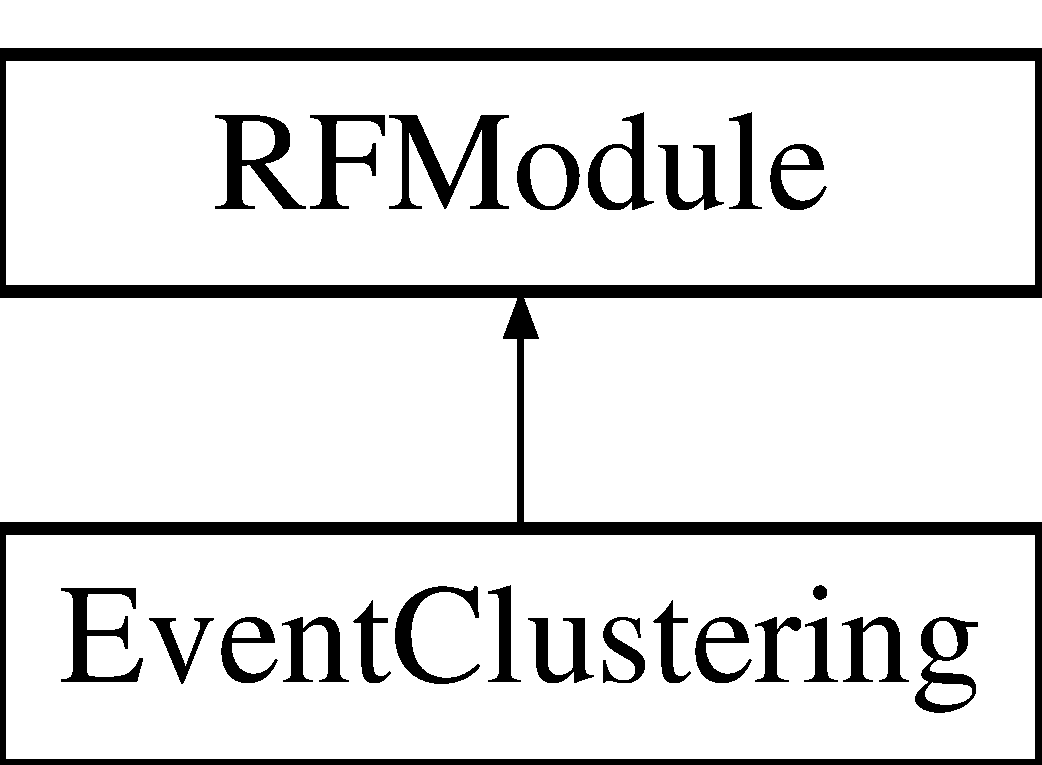
\includegraphics[height=2.000000cm]{classEventClustering}
\end{center}
\end{figure}
\subsection*{Public Member Functions}
\begin{DoxyCompactItemize}
\item 
bool {\bfseries configure} (yarp\+::os\+::\+Resource\+Finder \&rf)\hypertarget{classEventClustering_a9111f5db3d21a2a80bef0ac5a6996d06}{}\label{classEventClustering_a9111f5db3d21a2a80bef0ac5a6996d06}

\item 
bool {\bfseries interrupt\+Module} ()\hypertarget{classEventClustering_adb2bb1f480ac61629327d5170dd64398}{}\label{classEventClustering_adb2bb1f480ac61629327d5170dd64398}

\item 
bool {\bfseries close} ()\hypertarget{classEventClustering_af27e70c40cdfddab01c1fffed35620a3}{}\label{classEventClustering_af27e70c40cdfddab01c1fffed35620a3}

\item 
double {\bfseries get\+Period} ()\hypertarget{classEventClustering_afe356ead5fe50d67b2007e3f99f7818f}{}\label{classEventClustering_afe356ead5fe50d67b2007e3f99f7818f}

\item 
bool {\bfseries update\+Module} ()\hypertarget{classEventClustering_a25159637f1dc8c9cd27cde191b7296d2}{}\label{classEventClustering_a25159637f1dc8c9cd27cde191b7296d2}

\end{DoxyCompactItemize}


The documentation for this class was generated from the following files\+:\begin{DoxyCompactItemize}
\item 
/home/aglover/workspace/projects/event-\/driven/src/processing/v\+Cluster/include/event\+Clustering.\+h\item 
/home/aglover/workspace/projects/event-\/driven/src/processing/v\+Cluster/src/event\+Clustering.\+cpp\end{DoxyCompactItemize}

\hypertarget{classev_1_1fixedSurface}{}\section{ev\+:\+:fixed\+Surface Class Reference}
\label{classev_1_1fixedSurface}\index{ev\+::fixed\+Surface@{ev\+::fixed\+Surface}}


a spatio-\/temporal surface storing only a fixed number of events  




{\ttfamily \#include $<$v\+Window\+\_\+adv.\+h$>$}

Inheritance diagram for ev\+:\+:fixed\+Surface\+:\begin{figure}[H]
\begin{center}
\leavevmode
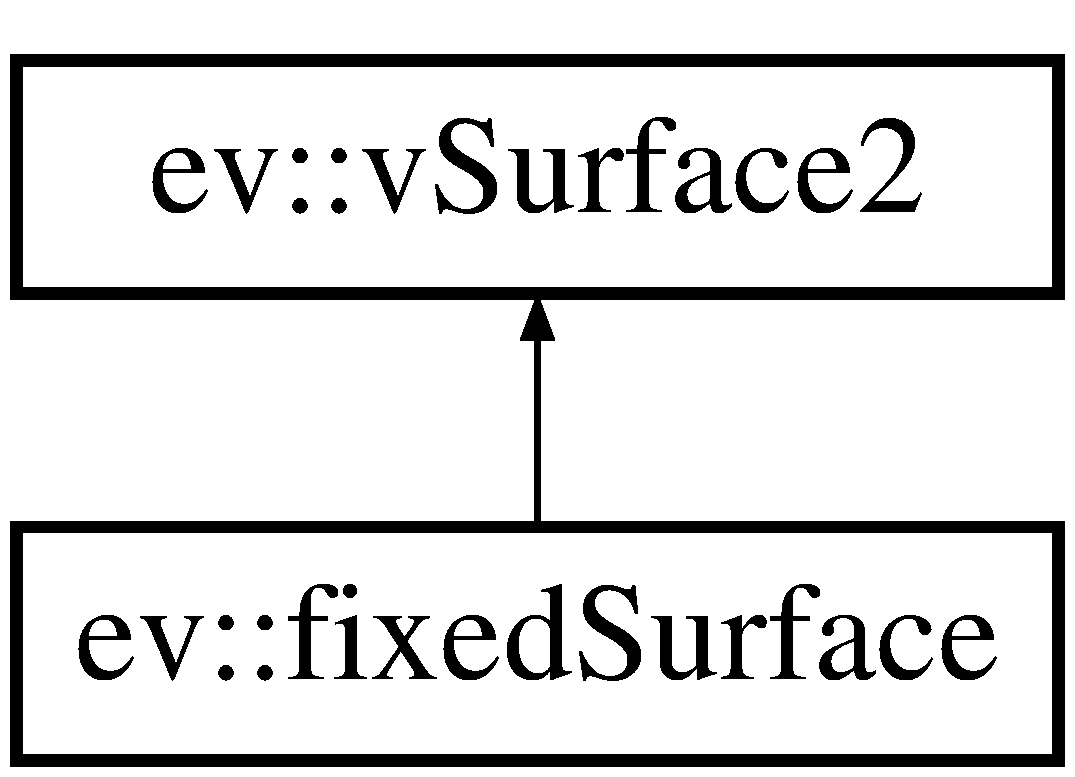
\includegraphics[height=2.000000cm]{classev_1_1fixedSurface}
\end{center}
\end{figure}
\subsection*{Public Member Functions}
\begin{DoxyCompactItemize}
\item 
{\bfseries fixed\+Surface} (int qlength=2000, int \hyperlink{classev_1_1vSurface2_a1aa8027816352a15d5b9bf1f26f48e76}{width}=128, int height=128)\hypertarget{classev_1_1fixedSurface_adee898e7c65c9c8d41fd20530d9f10b0}{}\label{classev_1_1fixedSurface_adee898e7c65c9c8d41fd20530d9f10b0}

\item 
virtual v\+Queue {\bfseries remove\+Events} (event$<$$>$ to\+Add)\hypertarget{classev_1_1fixedSurface_ace012acf57456f71d77fc7a349a915d7}{}\label{classev_1_1fixedSurface_ace012acf57456f71d77fc7a349a915d7}

\item 
virtual void {\bfseries fast\+Remove\+Events} (event$<$$>$ to\+Add)\hypertarget{classev_1_1fixedSurface_a317c375340f308fda67c6da2074f0e0e}{}\label{classev_1_1fixedSurface_a317c375340f308fda67c6da2074f0e0e}

\item 
void {\bfseries set\+Fixed\+Window\+Size} (int length)\hypertarget{classev_1_1fixedSurface_ac8249b63b5ada0491d6a6ff70b745488}{}\label{classev_1_1fixedSurface_ac8249b63b5ada0491d6a6ff70b745488}

\end{DoxyCompactItemize}
\subsection*{Additional Inherited Members}


\subsection{Detailed Description}
a spatio-\/temporal surface storing only a fixed number of events 

The documentation for this class was generated from the following files\+:\begin{DoxyCompactItemize}
\item 
/home/aglover/workspace/projects/event-\/driven/libraries/include/i\+Cub/eventdriven/v\+Window\+\_\+adv.\+h\item 
/home/aglover/workspace/projects/event-\/driven/libraries/src/v\+Window\+\_\+adv.\+cpp\end{DoxyCompactItemize}

\hypertarget{classflowDraw}{}\section{flow\+Draw Class Reference}
\label{classflowDraw}\index{flow\+Draw@{flow\+Draw}}
Inheritance diagram for flow\+Draw\+:\begin{figure}[H]
\begin{center}
\leavevmode
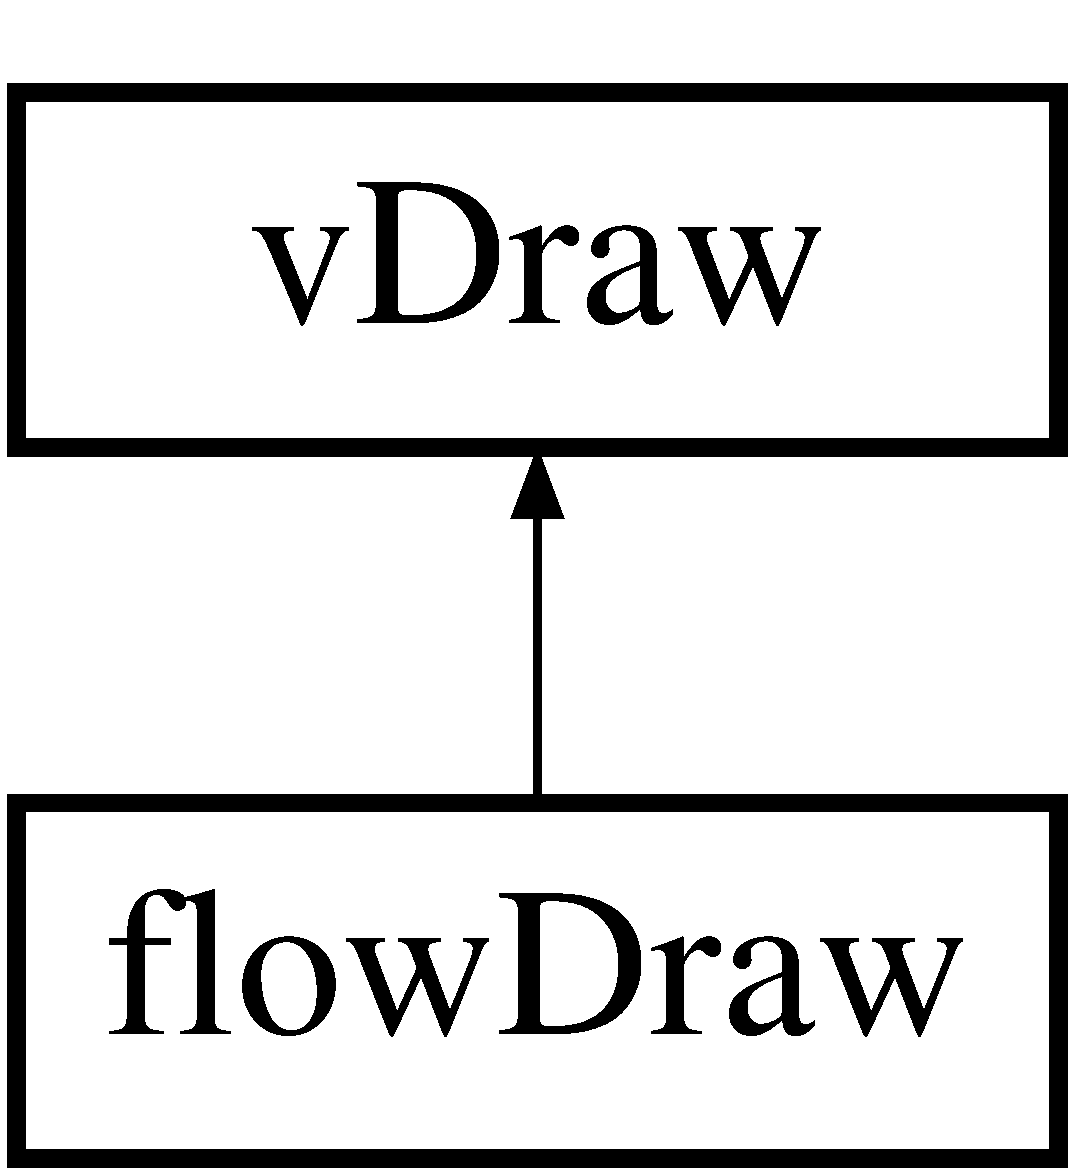
\includegraphics[height=2.000000cm]{classflowDraw}
\end{center}
\end{figure}
\subsection*{Public Member Functions}
\begin{DoxyCompactItemize}
\item 
virtual void \hyperlink{classflowDraw_a77d2abe2722b41f045bbea415ac0c858}{draw} (cv\+::\+Mat \&image, const ev\+::v\+Queue \&e\+Set, int v\+Time)
\begin{DoxyCompactList}\small\item\em draw takes an image and overlays the new visualisation textures \end{DoxyCompactList}\item 
virtual std\+::string \hyperlink{classflowDraw_a9b2f0523a05825d3d375b43126f6840e}{get\+Draw\+Type} ()
\begin{DoxyCompactList}\small\item\em get\+Tag returns the unique code for this drawing method. The arguments given on the command line must match this code exactly \end{DoxyCompactList}\item 
virtual std\+::string {\bfseries get\+Event\+Type} ()\hypertarget{classflowDraw_a9fd758baf18d8a518734b625521a188a}{}\label{classflowDraw_a9fd758baf18d8a518734b625521a188a}

\end{DoxyCompactItemize}
\subsection*{Static Public Attributes}
\begin{DoxyCompactItemize}
\item 
static const std\+::string {\bfseries drawtype} = \char`\"{}F\+L\+OW\char`\"{}\hypertarget{classflowDraw_a80a59d68527e7125aa574fde2970abeb}{}\label{classflowDraw_a80a59d68527e7125aa574fde2970abeb}

\end{DoxyCompactItemize}
\subsection*{Additional Inherited Members}


\subsection{Member Function Documentation}
\index{flow\+Draw@{flow\+Draw}!draw@{draw}}
\index{draw@{draw}!flow\+Draw@{flow\+Draw}}
\subsubsection[{\texorpdfstring{draw(cv\+::\+Mat \&image, const ev\+::v\+Queue \&e\+Set, int v\+Time)}{draw(cv::Mat &image, const ev::vQueue &eSet, int vTime)}}]{\setlength{\rightskip}{0pt plus 5cm}void flow\+Draw\+::draw (
\begin{DoxyParamCaption}
\item[{cv\+::\+Mat \&}]{canvas, }
\item[{const ev\+::v\+Queue \&}]{e\+Set, }
\item[{int}]{v\+Time}
\end{DoxyParamCaption}
)\hspace{0.3cm}{\ttfamily [virtual]}}\hypertarget{classflowDraw_a77d2abe2722b41f045bbea415ac0c858}{}\label{classflowDraw_a77d2abe2722b41f045bbea415ac0c858}


draw takes an image and overlays the new visualisation textures 


\begin{DoxyParams}{Parameters}
{\em canvas} & is the image which may or may not yet exist \\
\hline
{\em e\+Set} & is the set of events which could possibly be drawn \\
\hline
\end{DoxyParams}


Implements \hyperlink{classvDraw_a35cf7b42fe542fd51c1014de19fb114c}{v\+Draw}.

\index{flow\+Draw@{flow\+Draw}!get\+Draw\+Type@{get\+Draw\+Type}}
\index{get\+Draw\+Type@{get\+Draw\+Type}!flow\+Draw@{flow\+Draw}}
\subsubsection[{\texorpdfstring{get\+Draw\+Type()}{getDrawType()}}]{\setlength{\rightskip}{0pt plus 5cm}std\+::string flow\+Draw\+::get\+Draw\+Type (
\begin{DoxyParamCaption}
{}
\end{DoxyParamCaption}
)\hspace{0.3cm}{\ttfamily [virtual]}}\hypertarget{classflowDraw_a9b2f0523a05825d3d375b43126f6840e}{}\label{classflowDraw_a9b2f0523a05825d3d375b43126f6840e}


get\+Tag returns the unique code for this drawing method. The arguments given on the command line must match this code exactly 

\begin{DoxyReturn}{Returns}
the tag code 
\end{DoxyReturn}


Implements \hyperlink{classvDraw_abb4aa2bb3bb8daca40bdb12cd55d3fd3}{v\+Draw}.



The documentation for this class was generated from the following files\+:\begin{DoxyCompactItemize}
\item 
/home/aglover/workspace/projects/event-\/driven/src/processing/v\+Framer/include/v\+Draw.\+h\item 
/home/aglover/workspace/projects/event-\/driven/src/processing/v\+Framer/src/v\+Draw.\+cpp\end{DoxyCompactItemize}

\hypertarget{classev_1_1FlowEvent}{}\section{ev\+:\+:Flow\+Event Class Reference}
\label{classev_1_1FlowEvent}\index{ev\+::\+Flow\+Event@{ev\+::\+Flow\+Event}}


an \hyperlink{classev_1_1AddressEvent}{Address\+Event} with a velocity in visual space  




{\ttfamily \#include $<$v\+Codec.\+h$>$}

Inheritance diagram for ev\+:\+:Flow\+Event\+:\begin{figure}[H]
\begin{center}
\leavevmode
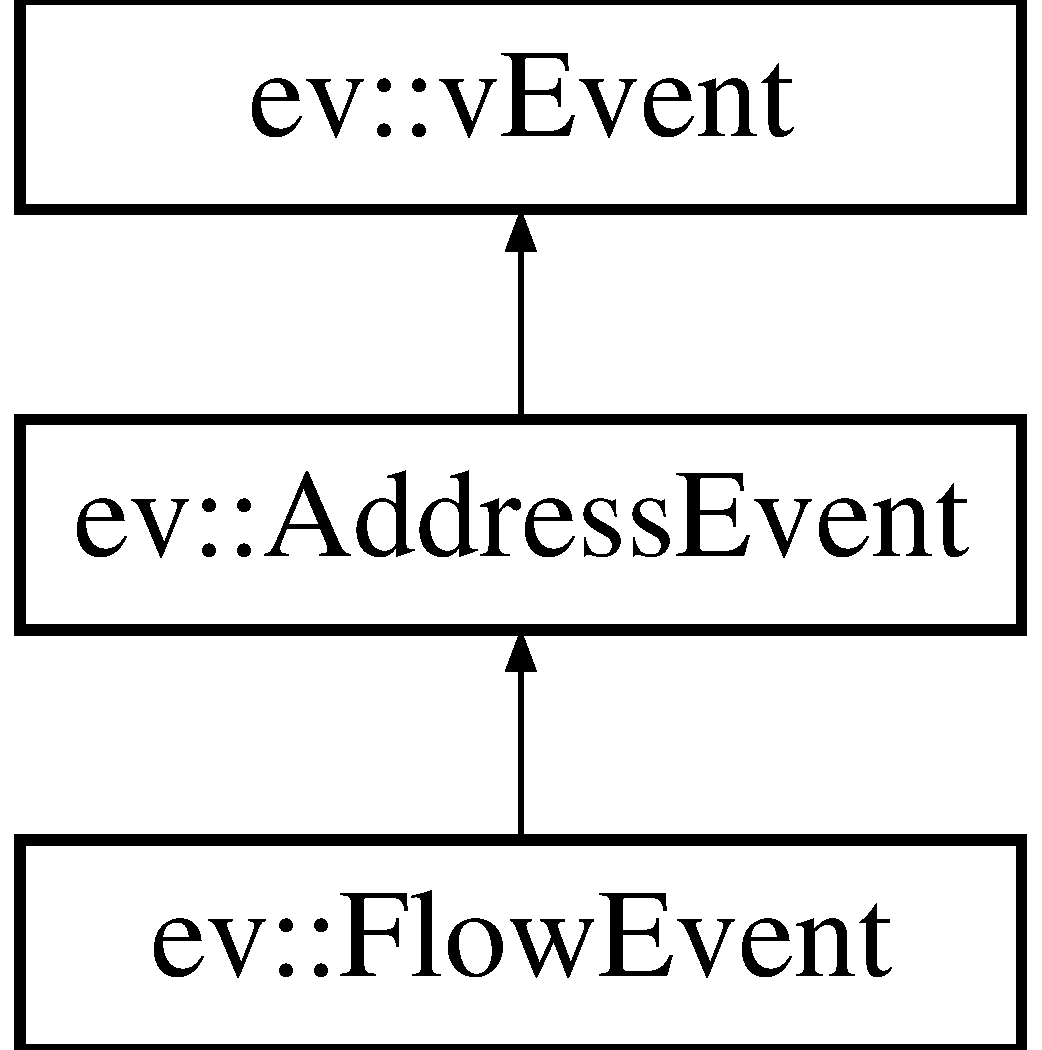
\includegraphics[height=3.000000cm]{classev_1_1FlowEvent}
\end{center}
\end{figure}
\subsection*{Public Member Functions}
\begin{DoxyCompactItemize}
\item 
{\bfseries Flow\+Event} (const \hyperlink{classev_1_1vEvent}{v\+Event} \&v)\hypertarget{classev_1_1FlowEvent_aa268bbbeb75a7ec0634e7eff9bf9dda5}{}\label{classev_1_1FlowEvent_aa268bbbeb75a7ec0634e7eff9bf9dda5}

\item 
{\bfseries Flow\+Event} (const \hyperlink{classev_1_1FlowEvent}{Flow\+Event} \&v)\hypertarget{classev_1_1FlowEvent_a0784e0ce0b0b1fb1d9c61f8134efa70b}{}\label{classev_1_1FlowEvent_a0784e0ce0b0b1fb1d9c61f8134efa70b}

\item 
virtual event {\bfseries clone} ()\hypertarget{classev_1_1FlowEvent_a6a108ba6028ea69a9398745074d7300f}{}\label{classev_1_1FlowEvent_a6a108ba6028ea69a9398745074d7300f}

\item 
virtual void {\bfseries encode} (yarp\+::os\+::\+Bottle \&b) const \hypertarget{classev_1_1FlowEvent_a13c900d7027a67d8197e32d56e92e0b0}{}\label{classev_1_1FlowEvent_a13c900d7027a67d8197e32d56e92e0b0}

\item 
virtual bool {\bfseries decode} (const yarp\+::os\+::\+Bottle \&packet, int \&pos)\hypertarget{classev_1_1FlowEvent_a47a44a03752d3d0b5de668bfa8092d43}{}\label{classev_1_1FlowEvent_a47a44a03752d3d0b5de668bfa8092d43}

\item 
virtual yarp\+::os\+::\+Property {\bfseries get\+Content} () const \hypertarget{classev_1_1FlowEvent_a299486f89e1f893a513d237fd70ba00c}{}\label{classev_1_1FlowEvent_a299486f89e1f893a513d237fd70ba00c}

\item 
virtual std\+::string {\bfseries get\+Type} () const \hypertarget{classev_1_1FlowEvent_a181159b6f05391e438b4a68908e572fb}{}\label{classev_1_1FlowEvent_a181159b6f05391e438b4a68908e572fb}

\item 
int {\bfseries get\+Death} () const \hypertarget{classev_1_1FlowEvent_ac39faf9016620faaddccd6c15b9f513f}{}\label{classev_1_1FlowEvent_ac39faf9016620faaddccd6c15b9f513f}

\end{DoxyCompactItemize}
\subsection*{Public Attributes}
\begin{DoxyCompactItemize}
\item 
float {\bfseries vx}\hypertarget{classev_1_1FlowEvent_a614490d12ab9767e546e2929a4c7a65e}{}\label{classev_1_1FlowEvent_a614490d12ab9767e546e2929a4c7a65e}

\item 
float {\bfseries vy}\hypertarget{classev_1_1FlowEvent_a20416e333c9f0258a2a1bbb49fb14989}{}\label{classev_1_1FlowEvent_a20416e333c9f0258a2a1bbb49fb14989}

\end{DoxyCompactItemize}
\subsection*{Static Public Attributes}
\begin{DoxyCompactItemize}
\item 
static const std\+::string {\bfseries tag} = \char`\"{}F\+L\+OW\char`\"{}\hypertarget{classev_1_1FlowEvent_a583ae9aaa6cbcbe1779eab526b5df1de}{}\label{classev_1_1FlowEvent_a583ae9aaa6cbcbe1779eab526b5df1de}

\end{DoxyCompactItemize}


\subsection{Detailed Description}
an \hyperlink{classev_1_1AddressEvent}{Address\+Event} with a velocity in visual space 

The documentation for this class was generated from the following files\+:\begin{DoxyCompactItemize}
\item 
/home/aglover/workspace/projects/event-\/driven/libraries/include/i\+Cub/eventdriven/v\+Codec.\+h\item 
/home/aglover/workspace/projects/event-\/driven/libraries/src/codecs/codec\+\_\+\+Flow\+Event.\+cpp\end{DoxyCompactItemize}

\hypertarget{structfpgaStatus}{}\section{fpga\+Status Struct Reference}
\label{structfpgaStatus}\index{fpga\+Status@{fpga\+Status}}
\subsection*{Public Attributes}
\begin{DoxyCompactItemize}
\item 
bool {\bfseries crc\+Err}\hypertarget{structfpgaStatus_a9cafcfd4e38fa240b31b47611bac3083}{}\label{structfpgaStatus_a9cafcfd4e38fa240b31b47611bac3083}

\item 
bool {\bfseries bias\+Done}\hypertarget{structfpgaStatus_aef80b6cd223b1195b317a70e7f57b58c}{}\label{structfpgaStatus_aef80b6cd223b1195b317a70e7f57b58c}

\item 
bool {\bfseries i2c\+Timeout}\hypertarget{structfpgaStatus_ab37e07a6f39e462634df9d560c0abe45}{}\label{structfpgaStatus_ab37e07a6f39e462634df9d560c0abe45}

\item 
bool {\bfseries aps\+Fifo\+Full}\hypertarget{structfpgaStatus_a01141df5867a1c152efd241a5341cfb7}{}\label{structfpgaStatus_a01141df5867a1c152efd241a5341cfb7}

\item 
bool {\bfseries td\+Fifo\+Full}\hypertarget{structfpgaStatus_a432c220a53f8a0639cb2b0ef1284ef14}{}\label{structfpgaStatus_a432c220a53f8a0639cb2b0ef1284ef14}

\end{DoxyCompactItemize}


The documentation for this struct was generated from the following file\+:\begin{DoxyCompactItemize}
\item 
/home/aglover/workspace/projects/event-\/driven/src/hardwareio/zynq\+Grabber/include/device\+Controller.\+h\end{DoxyCompactItemize}

\hypertarget{classgaborfilter}{}\section{gaborfilter Class Reference}
\label{classgaborfilter}\index{gaborfilter@{gaborfilter}}
\subsection*{Public Member Functions}
\begin{DoxyCompactItemize}
\item 
void {\bfseries set\+Center} (int cx, int cy)\hypertarget{classgaborfilter_ab851caaccfdec1ed1d1d49a93b5474a3}{}\label{classgaborfilter_ab851caaccfdec1ed1d1d49a93b5474a3}

\item 
void {\bfseries set\+Parameters} (double sigma, double stdsperlambda, double orientation, double disppx)\hypertarget{classgaborfilter_af246a88ffb2219f4a08bba2449f03d4c}{}\label{classgaborfilter_af246a88ffb2219f4a08bba2449f03d4c}

\item 
void {\bfseries set\+Complex} (bool complex=true)\hypertarget{classgaborfilter_a8b0747961e18733e0f6c266ef76f27f6}{}\label{classgaborfilter_a8b0747961e18733e0f6c266ef76f27f6}

\item 
void {\bfseries process} (\hyperlink{classev_1_1vEvent}{ev\+::v\+Event} \&evt, double gain=1.\+0)\hypertarget{classgaborfilter_aad471cb7dd8948b1cc266d5016be7510}{}\label{classgaborfilter_aad471cb7dd8948b1cc266d5016be7510}

\item 
void {\bfseries process} (ev\+::v\+Queue \&q, double gain=1.\+0)\hypertarget{classgaborfilter_ac92cb33f0d1a179a1b023f4f06d625f1}{}\label{classgaborfilter_ac92cb33f0d1a179a1b023f4f06d625f1}

\item 
double {\bfseries get\+Response} ()\hypertarget{classgaborfilter_a5db2373d31fb563fd560f7e1638f7af2}{}\label{classgaborfilter_a5db2373d31fb563fd560f7e1638f7af2}

\item 
void {\bfseries reset\+Response} ()\hypertarget{classgaborfilter_af3fec16a09439bf76c3df196285a28c0}{}\label{classgaborfilter_af3fec16a09439bf76c3df196285a28c0}

\end{DoxyCompactItemize}


The documentation for this class was generated from the following files\+:\begin{DoxyCompactItemize}
\item 
/home/aglover/workspace/projects/event-\/driven/src/applications/vergence\+Demo/vergence\+Controller/include/gaborfilters.\+h\item 
/home/aglover/workspace/projects/event-\/driven/src/applications/vergence\+Demo/vergence\+Controller/src/gaborfilters.\+cpp\end{DoxyCompactItemize}

\hypertarget{classev_1_1GaussianAE}{}\section{ev\+:\+:Gaussian\+AE Class Reference}
\label{classev_1_1GaussianAE}\index{ev\+::\+Gaussian\+AE@{ev\+::\+Gaussian\+AE}}


a \hyperlink{classev_1_1LabelledAE}{Labelled\+AE} with parameters that define a 2D gaussian  




{\ttfamily \#include $<$v\+Codec.\+h$>$}

Inheritance diagram for ev\+:\+:Gaussian\+AE\+:\begin{figure}[H]
\begin{center}
\leavevmode
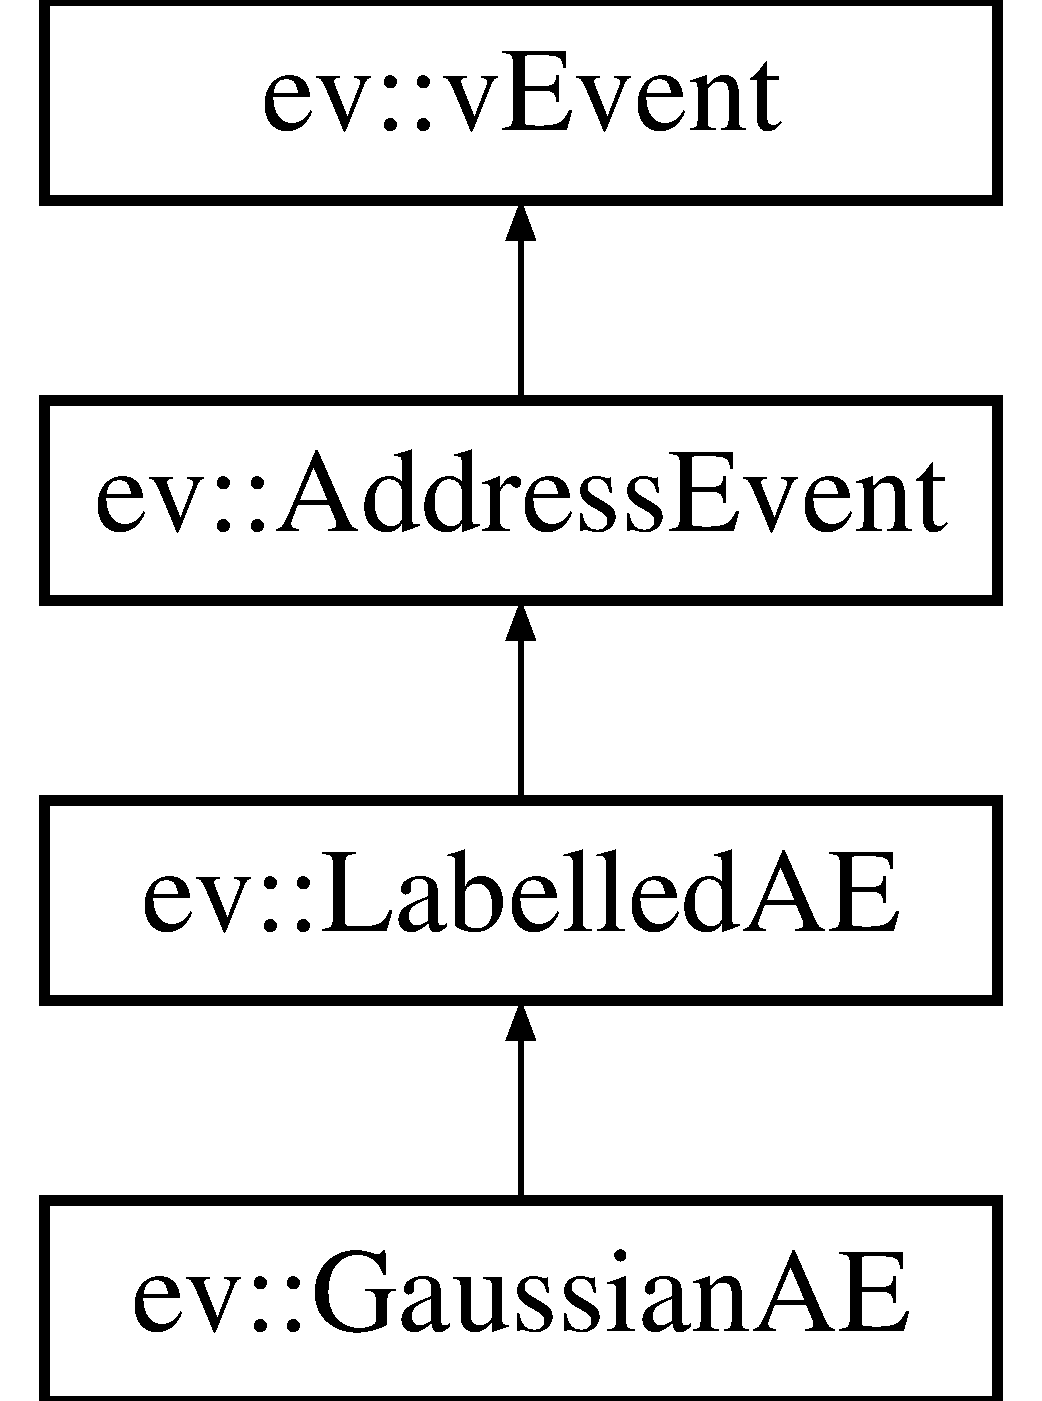
\includegraphics[height=4.000000cm]{classev_1_1GaussianAE}
\end{center}
\end{figure}
\subsection*{Public Member Functions}
\begin{DoxyCompactItemize}
\item 
{\bfseries Gaussian\+AE} (const \hyperlink{classev_1_1vEvent}{v\+Event} \&v)\hypertarget{classev_1_1GaussianAE_abc9c34d68ad44ea743b565a6206e591f}{}\label{classev_1_1GaussianAE_abc9c34d68ad44ea743b565a6206e591f}

\item 
{\bfseries Gaussian\+AE} (const \hyperlink{classev_1_1GaussianAE}{Gaussian\+AE} \&v)\hypertarget{classev_1_1GaussianAE_ac5934905f00cc08eb9c444f67e0ec6a2}{}\label{classev_1_1GaussianAE_ac5934905f00cc08eb9c444f67e0ec6a2}

\item 
virtual event {\bfseries clone} ()\hypertarget{classev_1_1GaussianAE_aa9e649d9039d3e9348cea99352df77c5}{}\label{classev_1_1GaussianAE_aa9e649d9039d3e9348cea99352df77c5}

\item 
virtual void {\bfseries encode} (yarp\+::os\+::\+Bottle \&b) const \hypertarget{classev_1_1GaussianAE_a305a85a18095be68f6ccef59bc1ee9a7}{}\label{classev_1_1GaussianAE_a305a85a18095be68f6ccef59bc1ee9a7}

\item 
virtual bool {\bfseries decode} (const yarp\+::os\+::\+Bottle \&packet, int \&pos)\hypertarget{classev_1_1GaussianAE_a7d673491b6b6e243d44131527c0ded39}{}\label{classev_1_1GaussianAE_a7d673491b6b6e243d44131527c0ded39}

\item 
virtual yarp\+::os\+::\+Property {\bfseries get\+Content} () const \hypertarget{classev_1_1GaussianAE_a986a28cb312c870c8e7fc1bc178a8a5a}{}\label{classev_1_1GaussianAE_a986a28cb312c870c8e7fc1bc178a8a5a}

\item 
virtual std\+::string {\bfseries get\+Type} () const \hypertarget{classev_1_1GaussianAE_a902ce886c1c5a2af42e073c3c7992bd5}{}\label{classev_1_1GaussianAE_a902ce886c1c5a2af42e073c3c7992bd5}

\end{DoxyCompactItemize}
\subsection*{Public Attributes}
\begin{DoxyCompactItemize}
\item 
float {\bfseries sigx}\hypertarget{classev_1_1GaussianAE_a2d4a7509a323da592be70372f41b09fe}{}\label{classev_1_1GaussianAE_a2d4a7509a323da592be70372f41b09fe}

\item 
float {\bfseries sigy}\hypertarget{classev_1_1GaussianAE_add6bf41b0ffbcbbecea6a63edb81b5b7}{}\label{classev_1_1GaussianAE_add6bf41b0ffbcbbecea6a63edb81b5b7}

\item 
float {\bfseries sigxy}\hypertarget{classev_1_1GaussianAE_a8d04e93f101622ce1f0240f0e02c5c90}{}\label{classev_1_1GaussianAE_a8d04e93f101622ce1f0240f0e02c5c90}

\end{DoxyCompactItemize}
\subsection*{Static Public Attributes}
\begin{DoxyCompactItemize}
\item 
static const std\+::string {\bfseries tag} = \char`\"{}G\+AE\char`\"{}\hypertarget{classev_1_1GaussianAE_a6d0ea5de274ddd380b056d2ba8b019e2}{}\label{classev_1_1GaussianAE_a6d0ea5de274ddd380b056d2ba8b019e2}

\end{DoxyCompactItemize}


\subsection{Detailed Description}
a \hyperlink{classev_1_1LabelledAE}{Labelled\+AE} with parameters that define a 2D gaussian 

The documentation for this class was generated from the following files\+:\begin{DoxyCompactItemize}
\item 
/home/aglover/workspace/projects/event-\/driven/libraries/include/i\+Cub/eventdriven/v\+Codec.\+h\item 
/home/aglover/workspace/projects/event-\/driven/libraries/src/codecs/codec\+\_\+\+Gaussian\+A\+E.\+cpp\end{DoxyCompactItemize}

\hypertarget{classev_1_1historicalSurface}{}\section{ev\+:\+:historical\+Surface Class Reference}
\label{classev_1_1historicalSurface}\index{ev\+::historical\+Surface@{ev\+::historical\+Surface}}
Inheritance diagram for ev\+:\+:historical\+Surface\+:\begin{figure}[H]
\begin{center}
\leavevmode
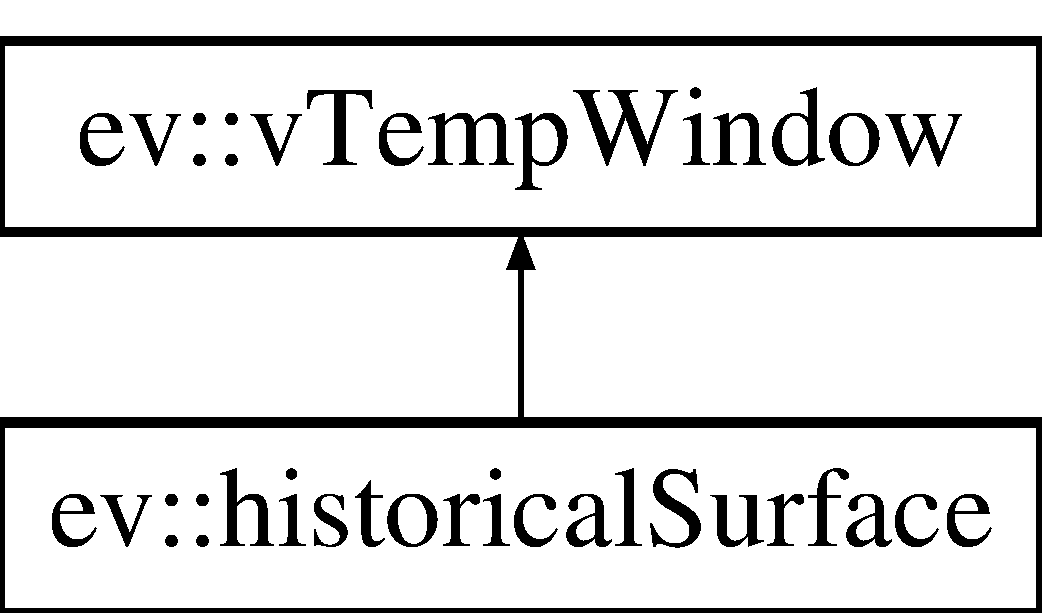
\includegraphics[height=2.000000cm]{classev_1_1historicalSurface}
\end{center}
\end{figure}
\subsection*{Public Member Functions}
\begin{DoxyCompactItemize}
\item 
void {\bfseries initialise} (int height, int width)\hypertarget{classev_1_1historicalSurface_adbe662bedcf6ee9c87f9b78d15c8ae85}{}\label{classev_1_1historicalSurface_adbe662bedcf6ee9c87f9b78d15c8ae85}

\item 
v\+Queue {\bfseries get\+Surface} (int query\+Time, int query\+Window)\hypertarget{classev_1_1historicalSurface_a03476e5a9cff0d369fef76711c6ebea5}{}\label{classev_1_1historicalSurface_a03476e5a9cff0d369fef76711c6ebea5}

\item 
v\+Queue {\bfseries get\+Surface} (int query\+Time, int query\+Window, int d)\hypertarget{classev_1_1historicalSurface_a289a2d3cb116fb1cdb99d38b03d74dd0}{}\label{classev_1_1historicalSurface_a289a2d3cb116fb1cdb99d38b03d74dd0}

\item 
v\+Queue {\bfseries get\+Surface} (int query\+Time, int query\+Window, int d, int x, int y)\hypertarget{classev_1_1historicalSurface_a10f0938bac2fc0b7a0f5624dfcd65f2f}{}\label{classev_1_1historicalSurface_a10f0938bac2fc0b7a0f5624dfcd65f2f}

\item 
v\+Queue {\bfseries get\+Surface} (int query\+Time, int query\+Window, int xl, int xh, int yl, int yh)\hypertarget{classev_1_1historicalSurface_a18830cb21753a190270bf03108c95f71}{}\label{classev_1_1historicalSurface_a18830cb21753a190270bf03108c95f71}

\end{DoxyCompactItemize}
\subsection*{Additional Inherited Members}


The documentation for this class was generated from the following files\+:\begin{DoxyCompactItemize}
\item 
/home/aglover/workspace/projects/event-\/driven/libraries/include/i\+Cub/eventdriven/v\+Window\+\_\+adv.\+h\item 
/home/aglover/workspace/projects/event-\/driven/libraries/src/v\+Window\+\_\+adv.\+cpp\end{DoxyCompactItemize}

\hypertarget{classev_1_1hSurfThread}{}\section{ev\+:\+:h\+Surf\+Thread Class Reference}
\label{classev_1_1hSurfThread}\index{ev\+::h\+Surf\+Thread@{ev\+::h\+Surf\+Thread}}


asynchronously read events and push them in a \hyperlink{classev_1_1historicalSurface}{historical\+Surface}  




{\ttfamily \#include $<$v\+Surface\+Handler\+Th.\+h$>$}

Inheritance diagram for ev\+:\+:h\+Surf\+Thread\+:\begin{figure}[H]
\begin{center}
\leavevmode
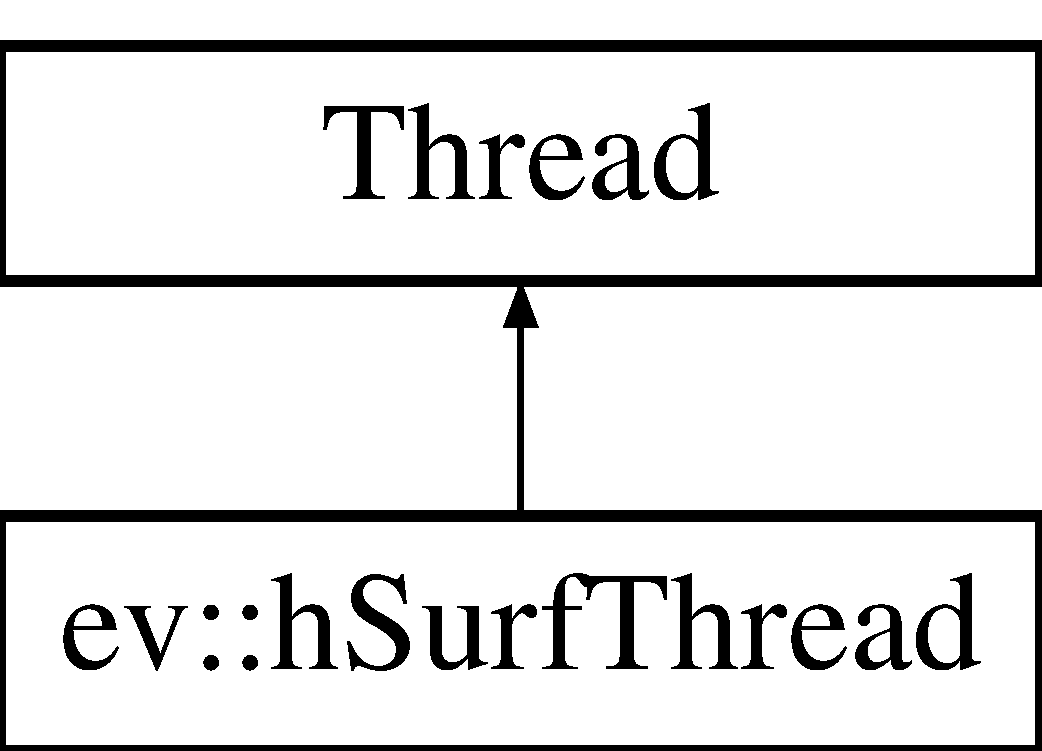
\includegraphics[height=2.000000cm]{classev_1_1hSurfThread}
\end{center}
\end{figure}
\subsection*{Public Member Functions}
\begin{DoxyCompactItemize}
\item 
void {\bfseries configure} (int height, int width, double maxcpudelay)\hypertarget{classev_1_1hSurfThread_a17acb3eb05f063ab81ab5128986ed7c8}{}\label{classev_1_1hSurfThread_a17acb3eb05f063ab81ab5128986ed7c8}

\item 
bool {\bfseries open} (std\+::string portname)\hypertarget{classev_1_1hSurfThread_afa2fc93ae2c64231e566738ebfddabf1}{}\label{classev_1_1hSurfThread_afa2fc93ae2c64231e566738ebfddabf1}

\item 
void {\bfseries on\+Stop} ()\hypertarget{classev_1_1hSurfThread_a7897b02f77738563c0d2fd5123dc4c51}{}\label{classev_1_1hSurfThread_a7897b02f77738563c0d2fd5123dc4c51}

\item 
void {\bfseries run} ()\hypertarget{classev_1_1hSurfThread_af4a0a8b35321419785dce1b94e43e5e3}{}\label{classev_1_1hSurfThread_af4a0a8b35321419785dce1b94e43e5e3}

\item 
v\+Queue {\bfseries query\+R\+OI} (int channel, unsigned int query\+Size, int x, int y, int r)\hypertarget{classev_1_1hSurfThread_ada4a11e319f5f0122897e21d6411bb1a}{}\label{classev_1_1hSurfThread_ada4a11e319f5f0122897e21d6411bb1a}

\item 
v\+Queue {\bfseries query\+Window} (int channel, unsigned int query\+Size)\hypertarget{classev_1_1hSurfThread_a89e485321978fdf785ba0e4e3b08a7ec}{}\label{classev_1_1hSurfThread_a89e485321978fdf785ba0e4e3b08a7ec}

\item 
double {\bfseries query\+Delay} (int channel=0)\hypertarget{classev_1_1hSurfThread_ae50c10e866f8692aae342d75e38369e7}{}\label{classev_1_1hSurfThread_ae50c10e866f8692aae342d75e38369e7}

\item 
yarp\+::os\+::\+Stamp {\bfseries query\+Ystamp} ()\hypertarget{classev_1_1hSurfThread_a02f2a70c6f8147e70e1689520555c389}{}\label{classev_1_1hSurfThread_a02f2a70c6f8147e70e1689520555c389}

\item 
int {\bfseries query\+Vstamp} (int channel=0)\hypertarget{classev_1_1hSurfThread_af5da61e8087f133f2202c873660779bc}{}\label{classev_1_1hSurfThread_af5da61e8087f133f2202c873660779bc}

\end{DoxyCompactItemize}


\subsection{Detailed Description}
asynchronously read events and push them in a \hyperlink{classev_1_1historicalSurface}{historical\+Surface} 

The documentation for this class was generated from the following file\+:\begin{DoxyCompactItemize}
\item 
/home/aglover/workspace/projects/event-\/driven/libraries/include/i\+Cub/eventdriven/v\+Surface\+Handler\+Th.\+h\end{DoxyCompactItemize}

\hypertarget{classinterestDraw}{}\section{interest\+Draw Class Reference}
\label{classinterestDraw}\index{interest\+Draw@{interest\+Draw}}
Inheritance diagram for interest\+Draw\+:\begin{figure}[H]
\begin{center}
\leavevmode
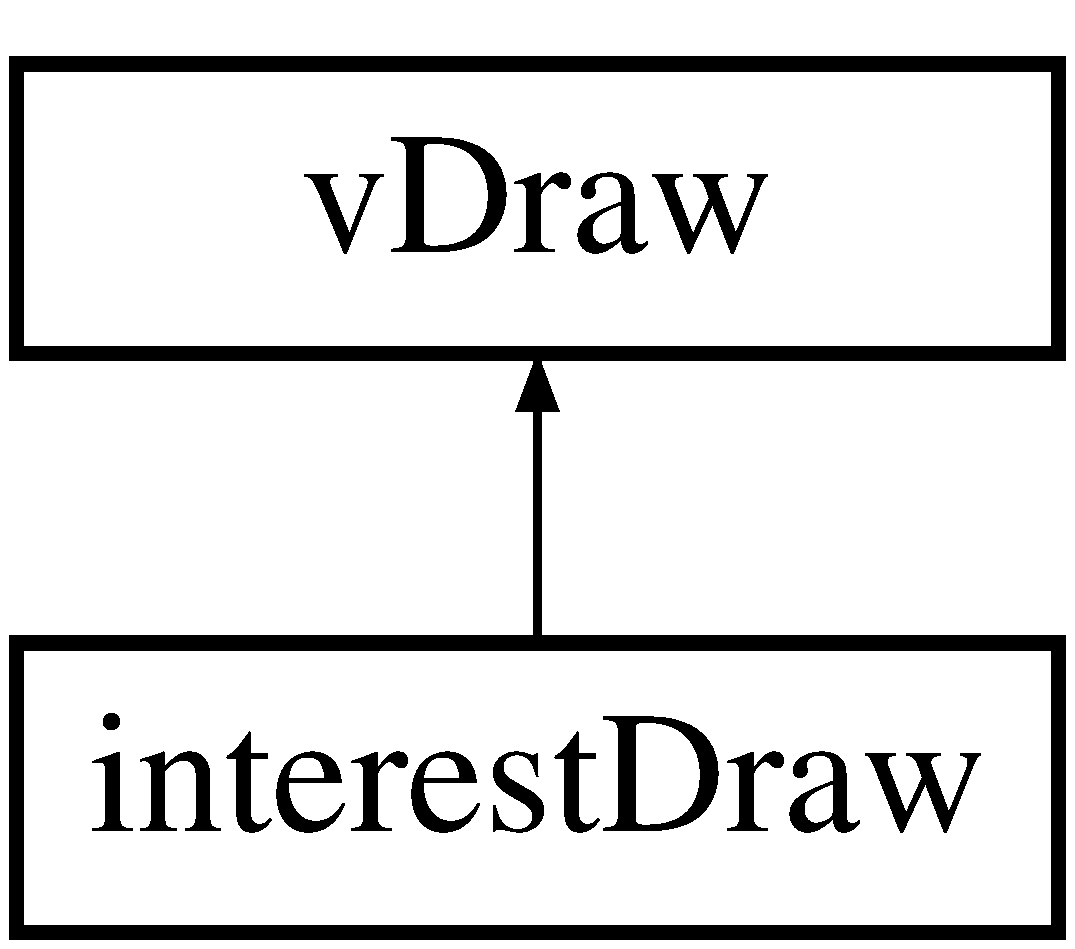
\includegraphics[height=2.000000cm]{classinterestDraw}
\end{center}
\end{figure}
\subsection*{Public Member Functions}
\begin{DoxyCompactItemize}
\item 
virtual void \hyperlink{classinterestDraw_a0e181779fcbc9303d2f6c77e5151eca8}{draw} (cv\+::\+Mat \&image, const ev\+::v\+Queue \&e\+Set, int v\+Time)
\begin{DoxyCompactList}\small\item\em draw takes an image and overlays the new visualisation textures \end{DoxyCompactList}\item 
virtual std\+::string \hyperlink{classinterestDraw_a8121cc47bf53a6571e6afcb1afe68d86}{get\+Draw\+Type} ()
\begin{DoxyCompactList}\small\item\em get\+Tag returns the unique code for this drawing method. The arguments given on the command line must match this code exactly \end{DoxyCompactList}\item 
virtual std\+::string {\bfseries get\+Event\+Type} ()\hypertarget{classinterestDraw_a9be4fecf2899af86ca32e0eaa137ae5e}{}\label{classinterestDraw_a9be4fecf2899af86ca32e0eaa137ae5e}

\end{DoxyCompactItemize}
\subsection*{Static Public Attributes}
\begin{DoxyCompactItemize}
\item 
static const std\+::string {\bfseries drawtype} = \char`\"{}AE-\/I\+NT\char`\"{}\hypertarget{classinterestDraw_ac439839e21e0d791d83ae245194e5629}{}\label{classinterestDraw_ac439839e21e0d791d83ae245194e5629}

\end{DoxyCompactItemize}
\subsection*{Additional Inherited Members}


\subsection{Member Function Documentation}
\index{interest\+Draw@{interest\+Draw}!draw@{draw}}
\index{draw@{draw}!interest\+Draw@{interest\+Draw}}
\subsubsection[{\texorpdfstring{draw(cv\+::\+Mat \&image, const ev\+::v\+Queue \&e\+Set, int v\+Time)}{draw(cv::Mat &image, const ev::vQueue &eSet, int vTime)}}]{\setlength{\rightskip}{0pt plus 5cm}void interest\+Draw\+::draw (
\begin{DoxyParamCaption}
\item[{cv\+::\+Mat \&}]{canvas, }
\item[{const ev\+::v\+Queue \&}]{e\+Set, }
\item[{int}]{v\+Time}
\end{DoxyParamCaption}
)\hspace{0.3cm}{\ttfamily [virtual]}}\hypertarget{classinterestDraw_a0e181779fcbc9303d2f6c77e5151eca8}{}\label{classinterestDraw_a0e181779fcbc9303d2f6c77e5151eca8}


draw takes an image and overlays the new visualisation textures 


\begin{DoxyParams}{Parameters}
{\em canvas} & is the image which may or may not yet exist \\
\hline
{\em e\+Set} & is the set of events which could possibly be drawn \\
\hline
\end{DoxyParams}


Implements \hyperlink{classvDraw_a35cf7b42fe542fd51c1014de19fb114c}{v\+Draw}.

\index{interest\+Draw@{interest\+Draw}!get\+Draw\+Type@{get\+Draw\+Type}}
\index{get\+Draw\+Type@{get\+Draw\+Type}!interest\+Draw@{interest\+Draw}}
\subsubsection[{\texorpdfstring{get\+Draw\+Type()}{getDrawType()}}]{\setlength{\rightskip}{0pt plus 5cm}std\+::string interest\+Draw\+::get\+Draw\+Type (
\begin{DoxyParamCaption}
{}
\end{DoxyParamCaption}
)\hspace{0.3cm}{\ttfamily [virtual]}}\hypertarget{classinterestDraw_a8121cc47bf53a6571e6afcb1afe68d86}{}\label{classinterestDraw_a8121cc47bf53a6571e6afcb1afe68d86}


get\+Tag returns the unique code for this drawing method. The arguments given on the command line must match this code exactly 

\begin{DoxyReturn}{Returns}
the tag code 
\end{DoxyReturn}


Implements \hyperlink{classvDraw_abb4aa2bb3bb8daca40bdb12cd55d3fd3}{v\+Draw}.



The documentation for this class was generated from the following files\+:\begin{DoxyCompactItemize}
\item 
/home/aglover/workspace/projects/event-\/driven/src/processing/v\+Framer/include/v\+Draw.\+h\item 
/home/aglover/workspace/projects/event-\/driven/src/processing/v\+Framer/src/v\+Draw.\+cpp\end{DoxyCompactItemize}

\hypertarget{classisoDraw}{}\section{iso\+Draw Class Reference}
\label{classisoDraw}\index{iso\+Draw@{iso\+Draw}}
Inheritance diagram for iso\+Draw\+:\begin{figure}[H]
\begin{center}
\leavevmode
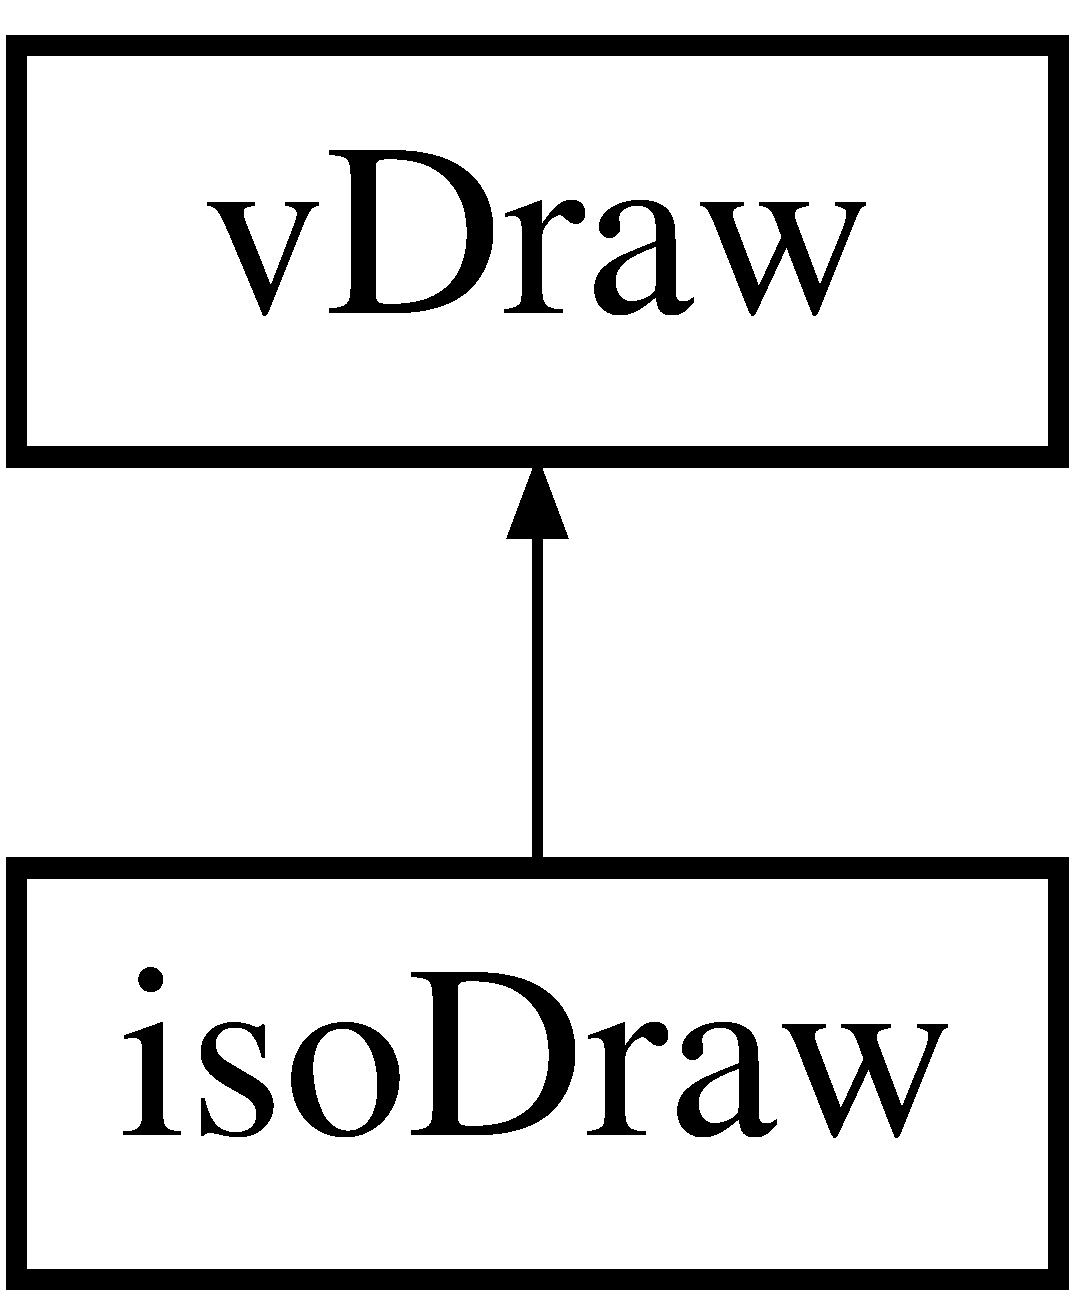
\includegraphics[height=2.000000cm]{classisoDraw}
\end{center}
\end{figure}
\subsection*{Public Member Functions}
\begin{DoxyCompactItemize}
\item 
void {\bfseries initialise} ()\hypertarget{classisoDraw_a3f77f51dbc01edb801d2c0f2a2c88fbf}{}\label{classisoDraw_a3f77f51dbc01edb801d2c0f2a2c88fbf}

\item 
virtual void \hyperlink{classisoDraw_a20877ef82deb90f2bdea5a3225fc447d}{draw} (cv\+::\+Mat \&image, const ev\+::v\+Queue \&e\+Set, int v\+Time)
\begin{DoxyCompactList}\small\item\em draw takes an image and overlays the new visualisation textures \end{DoxyCompactList}\item 
virtual std\+::string \hyperlink{classisoDraw_a8ff12e0ab9d2b65a16afc175c7cc59c1}{get\+Draw\+Type} ()
\begin{DoxyCompactList}\small\item\em get\+Tag returns the unique code for this drawing method. The arguments given on the command line must match this code exactly \end{DoxyCompactList}\item 
virtual std\+::string {\bfseries get\+Event\+Type} ()\hypertarget{classisoDraw_ade662b244b8de886f9f80c8928cc849b}{}\label{classisoDraw_ade662b244b8de886f9f80c8928cc849b}

\end{DoxyCompactItemize}
\subsection*{Static Public Attributes}
\begin{DoxyCompactItemize}
\item 
static const std\+::string {\bfseries drawtype} = \char`\"{}I\+SO\char`\"{}\hypertarget{classisoDraw_aa40d55a262ce4581da5391cf22cb39fd}{}\label{classisoDraw_aa40d55a262ce4581da5391cf22cb39fd}

\end{DoxyCompactItemize}
\subsection*{Additional Inherited Members}


\subsection{Member Function Documentation}
\index{iso\+Draw@{iso\+Draw}!draw@{draw}}
\index{draw@{draw}!iso\+Draw@{iso\+Draw}}
\subsubsection[{\texorpdfstring{draw(cv\+::\+Mat \&image, const ev\+::v\+Queue \&e\+Set, int v\+Time)}{draw(cv::Mat &image, const ev::vQueue &eSet, int vTime)}}]{\setlength{\rightskip}{0pt plus 5cm}void iso\+Draw\+::draw (
\begin{DoxyParamCaption}
\item[{cv\+::\+Mat \&}]{canvas, }
\item[{const ev\+::v\+Queue \&}]{e\+Set, }
\item[{int}]{v\+Time}
\end{DoxyParamCaption}
)\hspace{0.3cm}{\ttfamily [virtual]}}\hypertarget{classisoDraw_a20877ef82deb90f2bdea5a3225fc447d}{}\label{classisoDraw_a20877ef82deb90f2bdea5a3225fc447d}


draw takes an image and overlays the new visualisation textures 


\begin{DoxyParams}{Parameters}
{\em canvas} & is the image which may or may not yet exist \\
\hline
{\em e\+Set} & is the set of events which could possibly be drawn \\
\hline
\end{DoxyParams}


Implements \hyperlink{classvDraw_a35cf7b42fe542fd51c1014de19fb114c}{v\+Draw}.

\index{iso\+Draw@{iso\+Draw}!get\+Draw\+Type@{get\+Draw\+Type}}
\index{get\+Draw\+Type@{get\+Draw\+Type}!iso\+Draw@{iso\+Draw}}
\subsubsection[{\texorpdfstring{get\+Draw\+Type()}{getDrawType()}}]{\setlength{\rightskip}{0pt plus 5cm}std\+::string iso\+Draw\+::get\+Draw\+Type (
\begin{DoxyParamCaption}
{}
\end{DoxyParamCaption}
)\hspace{0.3cm}{\ttfamily [virtual]}}\hypertarget{classisoDraw_a8ff12e0ab9d2b65a16afc175c7cc59c1}{}\label{classisoDraw_a8ff12e0ab9d2b65a16afc175c7cc59c1}


get\+Tag returns the unique code for this drawing method. The arguments given on the command line must match this code exactly 

\begin{DoxyReturn}{Returns}
the tag code 
\end{DoxyReturn}


Implements \hyperlink{classvDraw_abb4aa2bb3bb8daca40bdb12cd55d3fd3}{v\+Draw}.



The documentation for this class was generated from the following files\+:\begin{DoxyCompactItemize}
\item 
/home/aglover/workspace/projects/event-\/driven/src/processing/v\+Framer/include/v\+Draw.\+h\item 
/home/aglover/workspace/projects/event-\/driven/src/processing/v\+Framer/src/v\+Draw.\+cpp\end{DoxyCompactItemize}

\hypertarget{classev_1_1LabelledAE}{}\section{ev\+:\+:Labelled\+AE Class Reference}
\label{classev_1_1LabelledAE}\index{ev\+::\+Labelled\+AE@{ev\+::\+Labelled\+AE}}


an \hyperlink{classev_1_1AddressEvent}{Address\+Event} with an ID or class label  




{\ttfamily \#include $<$v\+Codec.\+h$>$}

Inheritance diagram for ev\+:\+:Labelled\+AE\+:\begin{figure}[H]
\begin{center}
\leavevmode
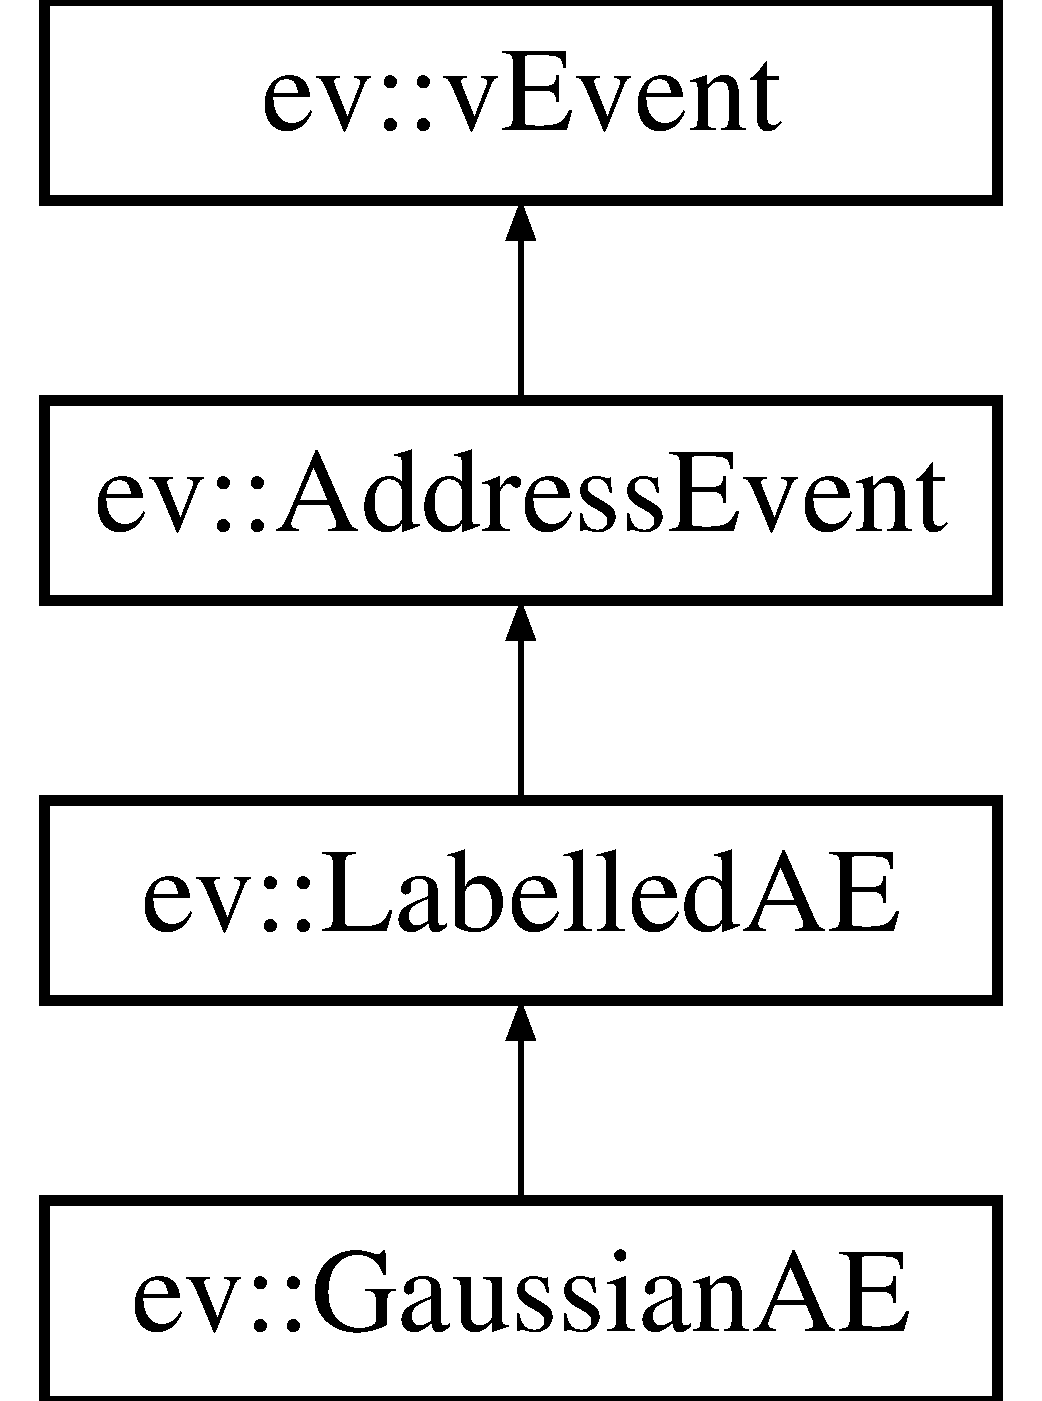
\includegraphics[height=4.000000cm]{classev_1_1LabelledAE}
\end{center}
\end{figure}
\subsection*{Public Member Functions}
\begin{DoxyCompactItemize}
\item 
{\bfseries Labelled\+AE} (const \hyperlink{classev_1_1vEvent}{v\+Event} \&v)\hypertarget{classev_1_1LabelledAE_ad9d765e87dbd81bddf3b58b7ba0f1b8a}{}\label{classev_1_1LabelledAE_ad9d765e87dbd81bddf3b58b7ba0f1b8a}

\item 
{\bfseries Labelled\+AE} (const \hyperlink{classev_1_1LabelledAE}{Labelled\+AE} \&v)\hypertarget{classev_1_1LabelledAE_aeca0ead752908e7c7f22aeb69b4f7e3a}{}\label{classev_1_1LabelledAE_aeca0ead752908e7c7f22aeb69b4f7e3a}

\item 
virtual event {\bfseries clone} ()\hypertarget{classev_1_1LabelledAE_aad6de4f38547d2b586c333de1c247ccf}{}\label{classev_1_1LabelledAE_aad6de4f38547d2b586c333de1c247ccf}

\item 
virtual void {\bfseries encode} (yarp\+::os\+::\+Bottle \&b) const \hypertarget{classev_1_1LabelledAE_a8e6ad790b6c44ca7482a073f594c1bf7}{}\label{classev_1_1LabelledAE_a8e6ad790b6c44ca7482a073f594c1bf7}

\item 
virtual bool {\bfseries decode} (const yarp\+::os\+::\+Bottle \&packet, int \&pos)\hypertarget{classev_1_1LabelledAE_a77cdc54c31f7998368a17277d2d6662a}{}\label{classev_1_1LabelledAE_a77cdc54c31f7998368a17277d2d6662a}

\item 
virtual yarp\+::os\+::\+Property {\bfseries get\+Content} () const \hypertarget{classev_1_1LabelledAE_acaf1c5db1cd5c1e639a151abd36ff57e}{}\label{classev_1_1LabelledAE_acaf1c5db1cd5c1e639a151abd36ff57e}

\item 
virtual std\+::string {\bfseries get\+Type} () const \hypertarget{classev_1_1LabelledAE_a331be65fc4ecb022ede92b02bff91ec6}{}\label{classev_1_1LabelledAE_a331be65fc4ecb022ede92b02bff91ec6}

\end{DoxyCompactItemize}
\subsection*{Public Attributes}
\begin{DoxyCompactItemize}
\item 
int {\bfseries ID}\hypertarget{classev_1_1LabelledAE_a59a295976cdf867006deea22d7cf1942}{}\label{classev_1_1LabelledAE_a59a295976cdf867006deea22d7cf1942}

\end{DoxyCompactItemize}
\subsection*{Static Public Attributes}
\begin{DoxyCompactItemize}
\item 
static const std\+::string {\bfseries tag} = \char`\"{}L\+AE\char`\"{}\hypertarget{classev_1_1LabelledAE_a825f9f0819046248ce7f6d0af4871cec}{}\label{classev_1_1LabelledAE_a825f9f0819046248ce7f6d0af4871cec}

\end{DoxyCompactItemize}


\subsection{Detailed Description}
an \hyperlink{classev_1_1AddressEvent}{Address\+Event} with an ID or class label 

The documentation for this class was generated from the following files\+:\begin{DoxyCompactItemize}
\item 
/home/aglover/workspace/projects/event-\/driven/libraries/include/i\+Cub/eventdriven/v\+Codec.\+h\item 
/home/aglover/workspace/projects/event-\/driven/libraries/src/codecs/codec\+\_\+\+Labelled\+A\+E.\+cpp\end{DoxyCompactItemize}

\hypertarget{classlifeDraw}{}\section{life\+Draw Class Reference}
\label{classlifeDraw}\index{life\+Draw@{life\+Draw}}
Inheritance diagram for life\+Draw\+:\begin{figure}[H]
\begin{center}
\leavevmode
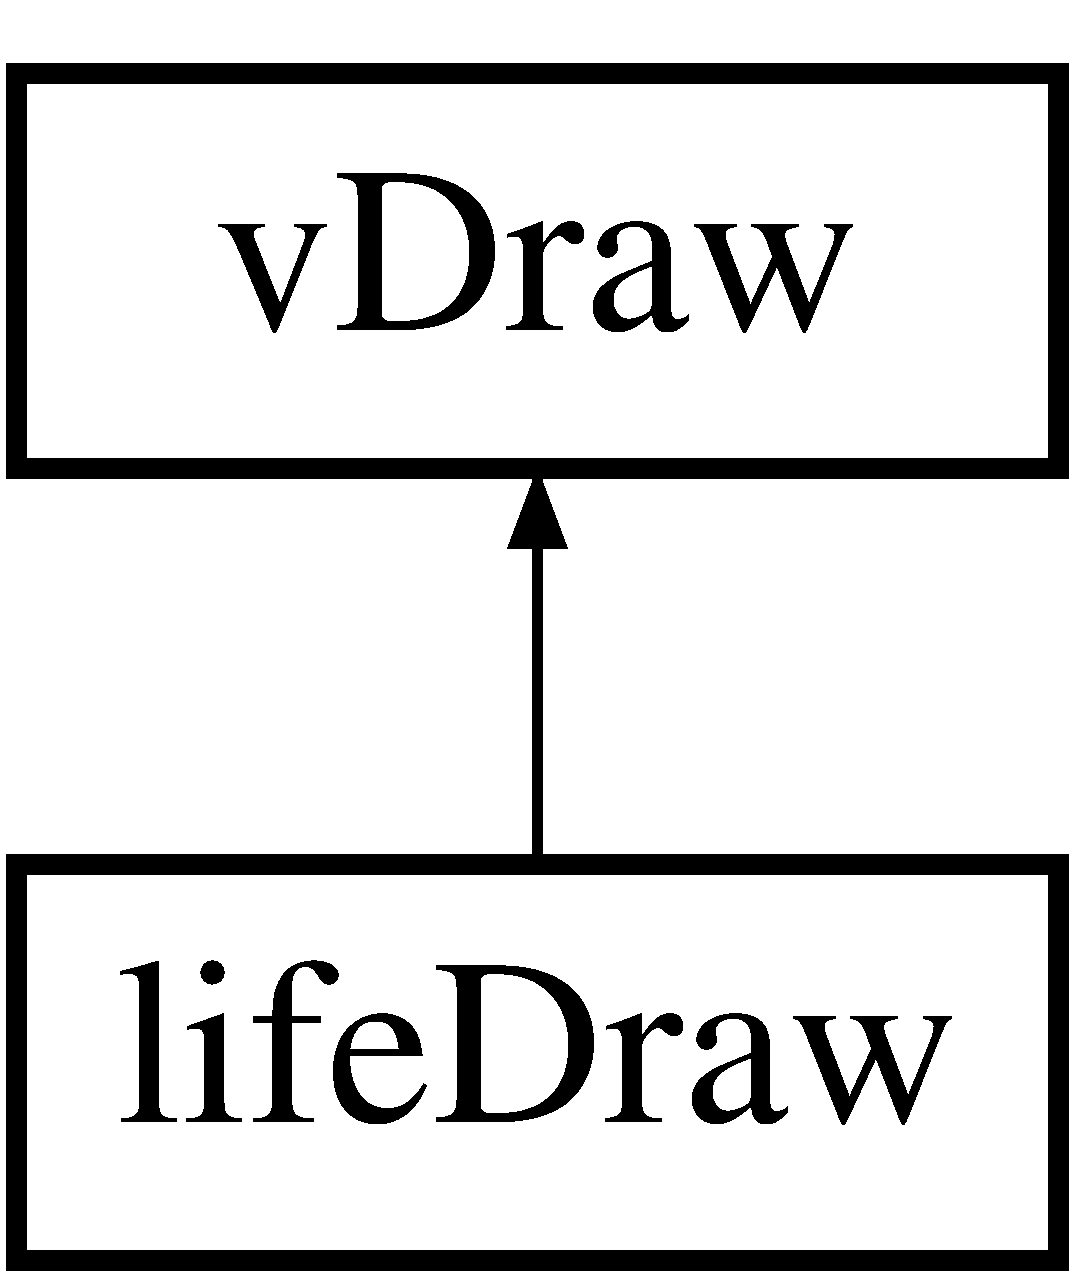
\includegraphics[height=2.000000cm]{classlifeDraw}
\end{center}
\end{figure}
\subsection*{Public Member Functions}
\begin{DoxyCompactItemize}
\item 
virtual void \hyperlink{classlifeDraw_af24592ae0bc8be55c7871e17adf6d77b}{draw} (cv\+::\+Mat \&image, const ev\+::v\+Queue \&e\+Set, int v\+Time)
\begin{DoxyCompactList}\small\item\em draw takes an image and overlays the new visualisation textures \end{DoxyCompactList}\item 
virtual std\+::string \hyperlink{classlifeDraw_a347b92eed9cd308902eecd3346eef5d4}{get\+Draw\+Type} ()
\begin{DoxyCompactList}\small\item\em get\+Tag returns the unique code for this drawing method. The arguments given on the command line must match this code exactly \end{DoxyCompactList}\item 
virtual std\+::string {\bfseries get\+Event\+Type} ()\hypertarget{classlifeDraw_a26a99ed97931f1c574f1366a9cbb848d}{}\label{classlifeDraw_a26a99ed97931f1c574f1366a9cbb848d}

\end{DoxyCompactItemize}
\subsection*{Static Public Attributes}
\begin{DoxyCompactItemize}
\item 
static const std\+::string {\bfseries drawtype} = \char`\"{}L\+I\+FE\char`\"{}\hypertarget{classlifeDraw_aac0bcaef3dd9be45ba6fe9df956f9b07}{}\label{classlifeDraw_aac0bcaef3dd9be45ba6fe9df956f9b07}

\end{DoxyCompactItemize}
\subsection*{Additional Inherited Members}


\subsection{Member Function Documentation}
\index{life\+Draw@{life\+Draw}!draw@{draw}}
\index{draw@{draw}!life\+Draw@{life\+Draw}}
\subsubsection[{\texorpdfstring{draw(cv\+::\+Mat \&image, const ev\+::v\+Queue \&e\+Set, int v\+Time)}{draw(cv::Mat &image, const ev::vQueue &eSet, int vTime)}}]{\setlength{\rightskip}{0pt plus 5cm}void life\+Draw\+::draw (
\begin{DoxyParamCaption}
\item[{cv\+::\+Mat \&}]{canvas, }
\item[{const ev\+::v\+Queue \&}]{e\+Set, }
\item[{int}]{v\+Time}
\end{DoxyParamCaption}
)\hspace{0.3cm}{\ttfamily [virtual]}}\hypertarget{classlifeDraw_af24592ae0bc8be55c7871e17adf6d77b}{}\label{classlifeDraw_af24592ae0bc8be55c7871e17adf6d77b}


draw takes an image and overlays the new visualisation textures 


\begin{DoxyParams}{Parameters}
{\em canvas} & is the image which may or may not yet exist \\
\hline
{\em e\+Set} & is the set of events which could possibly be drawn \\
\hline
\end{DoxyParams}


Implements \hyperlink{classvDraw_a35cf7b42fe542fd51c1014de19fb114c}{v\+Draw}.

\index{life\+Draw@{life\+Draw}!get\+Draw\+Type@{get\+Draw\+Type}}
\index{get\+Draw\+Type@{get\+Draw\+Type}!life\+Draw@{life\+Draw}}
\subsubsection[{\texorpdfstring{get\+Draw\+Type()}{getDrawType()}}]{\setlength{\rightskip}{0pt plus 5cm}std\+::string life\+Draw\+::get\+Draw\+Type (
\begin{DoxyParamCaption}
{}
\end{DoxyParamCaption}
)\hspace{0.3cm}{\ttfamily [virtual]}}\hypertarget{classlifeDraw_a347b92eed9cd308902eecd3346eef5d4}{}\label{classlifeDraw_a347b92eed9cd308902eecd3346eef5d4}


get\+Tag returns the unique code for this drawing method. The arguments given on the command line must match this code exactly 

\begin{DoxyReturn}{Returns}
the tag code 
\end{DoxyReturn}


Implements \hyperlink{classvDraw_abb4aa2bb3bb8daca40bdb12cd55d3fd3}{v\+Draw}.



The documentation for this class was generated from the following files\+:\begin{DoxyCompactItemize}
\item 
/home/aglover/workspace/projects/event-\/driven/src/processing/v\+Framer/include/v\+Draw.\+h\item 
/home/aglover/workspace/projects/event-\/driven/src/processing/v\+Framer/src/v\+Draw.\+cpp\end{DoxyCompactItemize}

\hypertarget{classev_1_1lifetimeSurface}{}\section{ev\+:\+:lifetime\+Surface Class Reference}
\label{classev_1_1lifetimeSurface}\index{ev\+::lifetime\+Surface@{ev\+::lifetime\+Surface}}


a spatio-\/temporal surface storing events for a \char`\"{}lifetime\char`\"{} given by the inverse of velocity  




{\ttfamily \#include $<$v\+Window\+\_\+adv.\+h$>$}

Inheritance diagram for ev\+:\+:lifetime\+Surface\+:\begin{figure}[H]
\begin{center}
\leavevmode
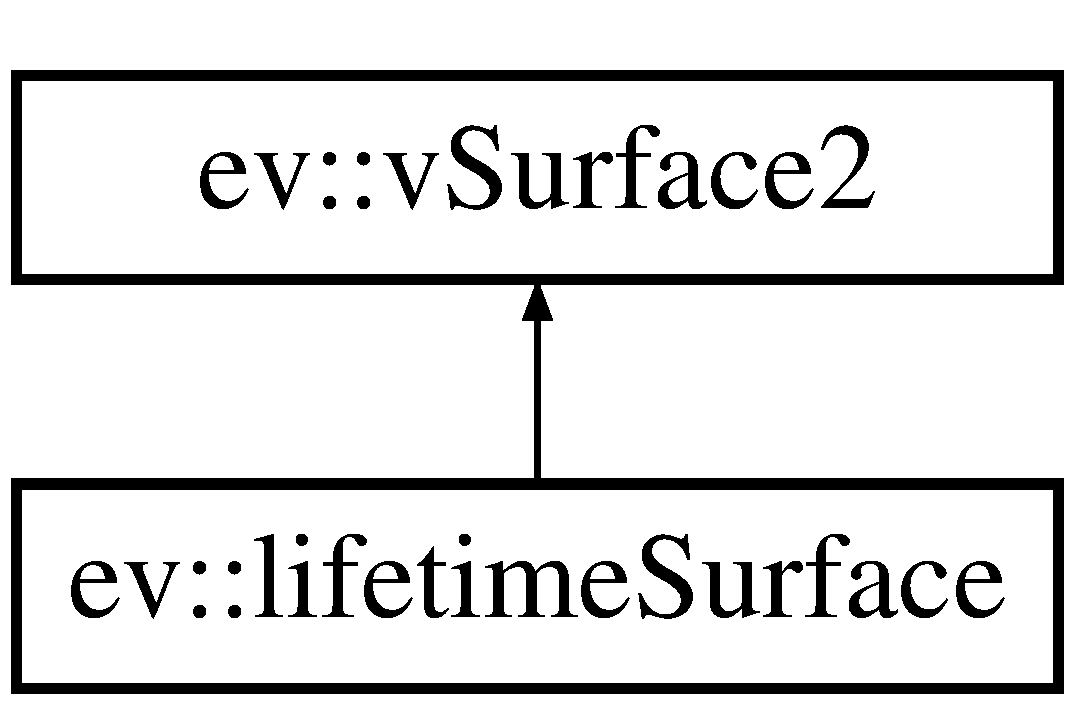
\includegraphics[height=2.000000cm]{classev_1_1lifetimeSurface}
\end{center}
\end{figure}
\subsection*{Public Member Functions}
\begin{DoxyCompactItemize}
\item 
{\bfseries lifetime\+Surface} (int \hyperlink{classev_1_1vSurface2_a1aa8027816352a15d5b9bf1f26f48e76}{width}=128, int height=128)\hypertarget{classev_1_1lifetimeSurface_a8276286d48b5baf2829268333f99b482}{}\label{classev_1_1lifetimeSurface_a8276286d48b5baf2829268333f99b482}

\item 
virtual v\+Queue \hyperlink{classev_1_1lifetimeSurface_a8fce037a13281c0e46c7d660e0ea2275}{add\+Event} (event$<$$>$ to\+Add)
\begin{DoxyCompactList}\small\item\em add\+Event adds an event to the window. Also checks for expired events. \end{DoxyCompactList}\item 
virtual v\+Queue {\bfseries remove\+Events} (event$<$$>$ to\+Add)\hypertarget{classev_1_1lifetimeSurface_a86fde904d007b5b1e5f52351bfab0b17}{}\label{classev_1_1lifetimeSurface_a86fde904d007b5b1e5f52351bfab0b17}

\item 
virtual void {\bfseries fast\+Remove\+Events} (event$<$$>$ to\+Add)\hypertarget{classev_1_1lifetimeSurface_a5502828fe59c4394588acb6ffa06d445}{}\label{classev_1_1lifetimeSurface_a5502828fe59c4394588acb6ffa06d445}

\end{DoxyCompactItemize}
\subsection*{Additional Inherited Members}


\subsection{Detailed Description}
a spatio-\/temporal surface storing events for a \char`\"{}lifetime\char`\"{} given by the inverse of velocity 

\subsection{Member Function Documentation}
\index{ev\+::lifetime\+Surface@{ev\+::lifetime\+Surface}!add\+Event@{add\+Event}}
\index{add\+Event@{add\+Event}!ev\+::lifetime\+Surface@{ev\+::lifetime\+Surface}}
\subsubsection[{\texorpdfstring{add\+Event(event$<$$>$ to\+Add)}{addEvent(event<> toAdd)}}]{\setlength{\rightskip}{0pt plus 5cm}v\+Queue ev\+::lifetime\+Surface\+::add\+Event (
\begin{DoxyParamCaption}
\item[{event$<$$>$}]{v}
\end{DoxyParamCaption}
)\hspace{0.3cm}{\ttfamily [virtual]}}\hypertarget{classev_1_1lifetimeSurface_a8fce037a13281c0e46c7d660e0ea2275}{}\label{classev_1_1lifetimeSurface_a8fce037a13281c0e46c7d660e0ea2275}


add\+Event adds an event to the window. Also checks for expired events. 


\begin{DoxyParams}{Parameters}
{\em event} & the event to add \\
\hline
\end{DoxyParams}


Reimplemented from \hyperlink{classev_1_1vSurface2_a6dee662976048b73d7b19e45871352da}{ev\+::v\+Surface2}.



The documentation for this class was generated from the following files\+:\begin{DoxyCompactItemize}
\item 
/home/aglover/workspace/projects/event-\/driven/libraries/include/i\+Cub/eventdriven/v\+Window\+\_\+adv.\+h\item 
/home/aglover/workspace/projects/event-\/driven/libraries/src/v\+Window\+\_\+adv.\+cpp\end{DoxyCompactItemize}

\hypertarget{classparticleProcessor}{}\section{particle\+Processor Class Reference}
\label{classparticleProcessor}\index{particle\+Processor@{particle\+Processor}}
Inheritance diagram for particle\+Processor\+:\begin{figure}[H]
\begin{center}
\leavevmode
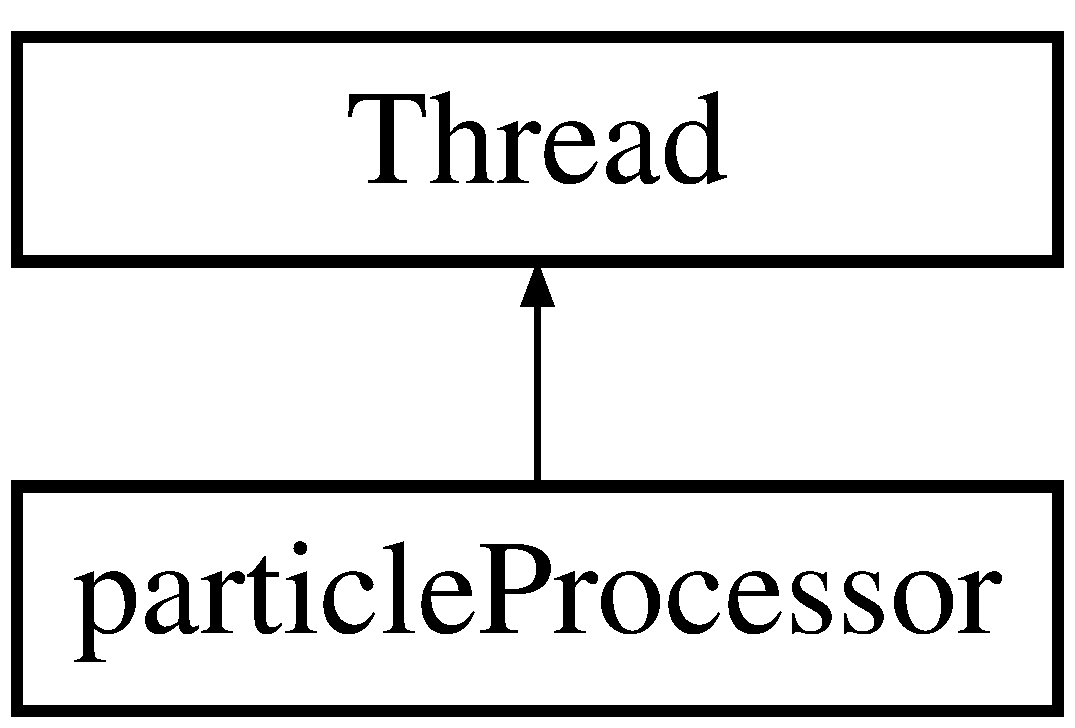
\includegraphics[height=2.000000cm]{classparticleProcessor}
\end{center}
\end{figure}
\subsection*{Public Member Functions}
\begin{DoxyCompactItemize}
\item 
void {\bfseries set\+Compute\+Options} (int camera, int threads, bool use\+R\+OI)\hypertarget{classparticleProcessor_a9ca07fccef931f0a6a82efe058285886}{}\label{classparticleProcessor_a9ca07fccef931f0a6a82efe058285886}

\item 
void {\bfseries set\+Filter\+Parameters} (int n\+Particles, double n\+Randomise, bool adaptive, double variance)\hypertarget{classparticleProcessor_ab7ef098114f6971f0bc24b6556a499b6}{}\label{classparticleProcessor_ab7ef098114f6971f0bc24b6556a499b6}

\item 
void {\bfseries set\+Observation\+Parameters} (double min\+Likelihood, double inlier\+Par, double outlier\+Par)\hypertarget{classparticleProcessor_a77cc8d09e8b52120dc98ac7e3ea89f48}{}\label{classparticleProcessor_a77cc8d09e8b52120dc98ac7e3ea89f48}

\item 
void {\bfseries set\+Seed} (double x, double y, double r)\hypertarget{classparticleProcessor_a520f0f6ab1afc01569c5e14cd4426197}{}\label{classparticleProcessor_a520f0f6ab1afc01569c5e14cd4426197}

\item 
{\bfseries particle\+Processor} (std\+::string name, unsigned int height, unsigned int width, \hyperlink{classev_1_1hSurfThread}{h\+Surf\+Thread} $\ast$eventhandler, \hyperlink{classev_1_1collectorPort}{collector\+Port} $\ast$eventsender)\hypertarget{classparticleProcessor_ac3f2ff8cbd65c236adc91dc3349cd611}{}\label{classparticleProcessor_ac3f2ff8cbd65c236adc91dc3349cd611}

\item 
bool {\bfseries thread\+Init} ()\hypertarget{classparticleProcessor_aafa6595892c7e82b1c42b919dfe6f9f0}{}\label{classparticleProcessor_aafa6595892c7e82b1c42b919dfe6f9f0}

\item 
void {\bfseries run} ()\hypertarget{classparticleProcessor_aed880e77fafb61965d57565735939181}{}\label{classparticleProcessor_aed880e77fafb61965d57565735939181}

\item 
void {\bfseries thread\+Release} ()\hypertarget{classparticleProcessor_ae40c3b11945587c4c23547d7b817299a}{}\label{classparticleProcessor_ae40c3b11945587c4c23547d7b817299a}

\end{DoxyCompactItemize}


The documentation for this class was generated from the following files\+:\begin{DoxyCompactItemize}
\item 
/home/aglover/workspace/projects/event-\/driven/src/processing/v\+Particle\+Filter/include/v\+Real\+Time.\+h\item 
/home/aglover/workspace/projects/event-\/driven/src/processing/v\+Particle\+Filter/src/v\+Real\+Time.\+cpp\end{DoxyCompactItemize}

\hypertarget{classpositionReader}{}\section{position\+Reader Class Reference}
\label{classpositionReader}\index{position\+Reader@{position\+Reader}}
Inheritance diagram for position\+Reader\+:\begin{figure}[H]
\begin{center}
\leavevmode
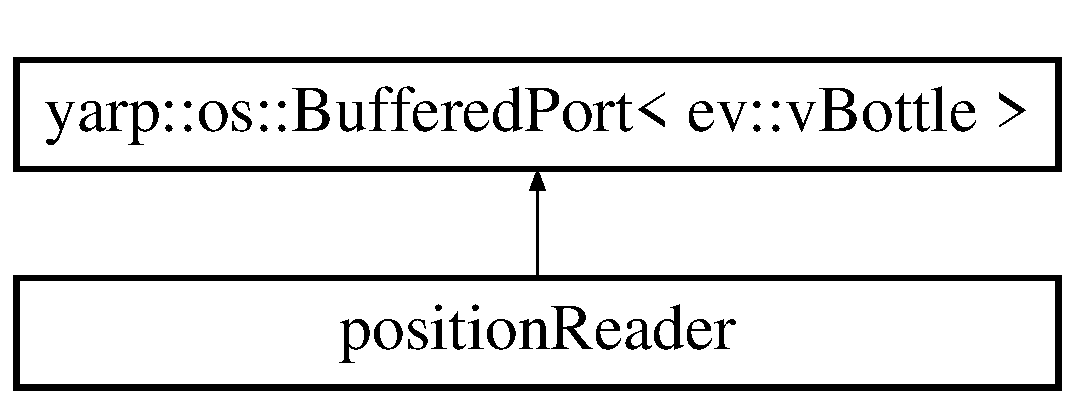
\includegraphics[height=2.000000cm]{classpositionReader}
\end{center}
\end{figure}
\subsection*{Public Member Functions}
\begin{DoxyCompactItemize}
\item 
void {\bfseries on\+Read} (\hyperlink{classev_1_1vBottle}{v\+Bottle} \&v\+Bottle\+In)\hypertarget{classpositionReader_a0cc3a67998f2205a786794730250b9c2}{}\label{classpositionReader_a0cc3a67998f2205a786794730250b9c2}

\item 
void {\bfseries get\+Targets} (yarp\+::sig\+::\+Vector \&left, yarp\+::sig\+::\+Vector \&right)\hypertarget{classpositionReader_a9f4f82b17b54dd6776eb29269ab043ce}{}\label{classpositionReader_a9f4f82b17b54dd6776eb29269ab043ce}

\end{DoxyCompactItemize}


The documentation for this class was generated from the following file\+:\begin{DoxyCompactItemize}
\item 
/home/aglover/workspace/projects/event-\/driven/src/applications/gaze\+Demo/include/v\+Track\+To\+Robot.\+h\end{DoxyCompactItemize}

\hypertarget{classpreComputedBins}{}\section{pre\+Computed\+Bins Class Reference}
\label{classpreComputedBins}\index{pre\+Computed\+Bins@{pre\+Computed\+Bins}}
\subsection*{Public Member Functions}
\begin{DoxyCompactItemize}
\item 
void {\bfseries configure} (int height, int width, double maxrad, int n\+Bins)\hypertarget{classpreComputedBins_af0d406410d46d3eddcb766987f926017}{}\label{classpreComputedBins_af0d406410d46d3eddcb766987f926017}

\item 
double {\bfseries query\+Distance} (int dy, int dx)\hypertarget{classpreComputedBins_aa40481ace2002018d665d1909a09f7b4}{}\label{classpreComputedBins_aa40481ace2002018d665d1909a09f7b4}

\item 
int {\bfseries query\+Bin\+Number} (double dy, double dx)\hypertarget{classpreComputedBins_ac54c38ccabf80894345145b6bc0bf508}{}\label{classpreComputedBins_ac54c38ccabf80894345145b6bc0bf508}

\end{DoxyCompactItemize}


The documentation for this class was generated from the following file\+:\begin{DoxyCompactItemize}
\item 
/home/aglover/workspace/projects/event-\/driven/src/processing/v\+Particle\+Filter/include/v\+Particle.\+h\end{DoxyCompactItemize}

\hypertarget{classev_1_1queueAllocator}{}\section{ev\+:\+:queue\+Allocator Class Reference}
\label{classev_1_1queueAllocator}\index{ev\+::queue\+Allocator@{ev\+::queue\+Allocator}}


an asynchronous reading port that accepts v\+Bottles and decodes them  




{\ttfamily \#include $<$v\+Surface\+Handler\+Th.\+h$>$}

Inheritance diagram for ev\+:\+:queue\+Allocator\+:\begin{figure}[H]
\begin{center}
\leavevmode
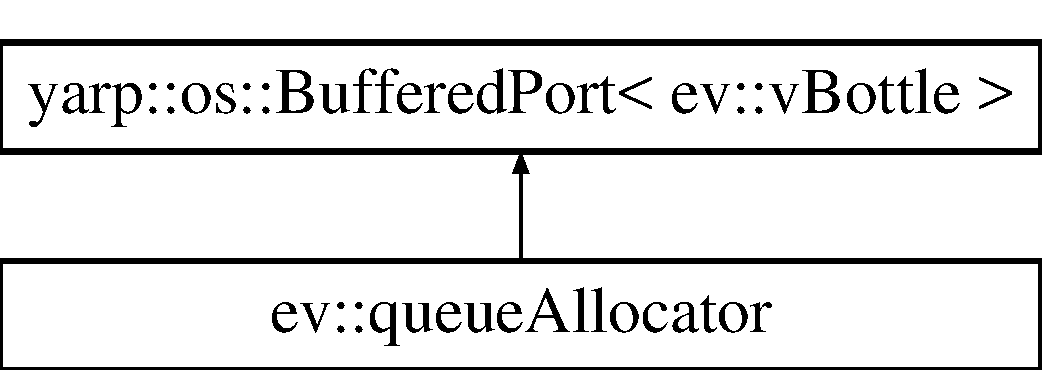
\includegraphics[height=2.000000cm]{classev_1_1queueAllocator}
\end{center}
\end{figure}
\subsection*{Public Member Functions}
\begin{DoxyCompactItemize}
\item 
void {\bfseries on\+Read} (\hyperlink{classev_1_1vBottle}{ev\+::v\+Bottle} \&inputbottle)\hypertarget{classev_1_1queueAllocator_a12ae388a8d2deb71ca5b927c3eb0a860}{}\label{classev_1_1queueAllocator_a12ae388a8d2deb71ca5b927c3eb0a860}

\item 
ev\+::v\+Queue $\ast$ {\bfseries get\+NextQ} (yarp\+::os\+::\+Stamp \&yarpstamp)\hypertarget{classev_1_1queueAllocator_a2429870a8dd1a2e1b71853bdc7a50bde}{}\label{classev_1_1queueAllocator_a2429870a8dd1a2e1b71853bdc7a50bde}

\item 
void {\bfseries scrapQ} ()\hypertarget{classev_1_1queueAllocator_a1a914bc39f534dc50a7eb2ba846753bf}{}\label{classev_1_1queueAllocator_a1a914bc39f534dc50a7eb2ba846753bf}

\item 
void {\bfseries release\+Data\+Lock} ()\hypertarget{classev_1_1queueAllocator_aa3ab79f1da7f2930811ab980347b0305}{}\label{classev_1_1queueAllocator_aa3ab79f1da7f2930811ab980347b0305}

\end{DoxyCompactItemize}


\subsection{Detailed Description}
an asynchronous reading port that accepts v\+Bottles and decodes them 

The documentation for this class was generated from the following file\+:\begin{DoxyCompactItemize}
\item 
/home/aglover/workspace/projects/event-\/driven/libraries/include/i\+Cub/eventdriven/v\+Surface\+Handler\+Th.\+h\end{DoxyCompactItemize}

\hypertarget{structev_1_1resolution}{}\section{ev\+:\+:resolution Struct Reference}
\label{structev_1_1resolution}\index{ev\+::resolution@{ev\+::resolution}}


an efficient structure for storing sensor resolution  




{\ttfamily \#include $<$vts\+Helper.\+h$>$}

\subsection*{Public Attributes}
\begin{DoxyCompactItemize}
\item 
unsigned int {\bfseries width}\+:10\hypertarget{structev_1_1resolution_af63d9f023bf48b5170fbde6fac1fa60d}{}\label{structev_1_1resolution_af63d9f023bf48b5170fbde6fac1fa60d}

\item 
unsigned int {\bfseries height}\+:10\hypertarget{structev_1_1resolution_ae9919e691ce05e1bbbf281dd79102ddb}{}\label{structev_1_1resolution_ae9919e691ce05e1bbbf281dd79102ddb}

\end{DoxyCompactItemize}


\subsection{Detailed Description}
an efficient structure for storing sensor resolution 

The documentation for this struct was generated from the following file\+:\begin{DoxyCompactItemize}
\item 
/home/aglover/workspace/projects/event-\/driven/libraries/include/i\+Cub/eventdriven/vts\+Helper.\+h\end{DoxyCompactItemize}

\hypertarget{classsobelfilter}{}\section{sobelfilter Class Reference}
\label{classsobelfilter}\index{sobelfilter@{sobelfilter}}
\subsection*{Public Member Functions}
\begin{DoxyCompactItemize}
\item 
void {\bfseries set\+Center} (int cx, int cy)\hypertarget{classsobelfilter_ab94731a7cf23f308ba8bff515e74da08}{}\label{classsobelfilter_ab94731a7cf23f308ba8bff515e74da08}

\item 
void {\bfseries set\+Sobel\+Filters} (int sobelsize)\hypertarget{classsobelfilter_a1e6e42100581b793b998f65584eae393}{}\label{classsobelfilter_a1e6e42100581b793b998f65584eae393}

\item 
int {\bfseries factorial} (int a)\hypertarget{classsobelfilter_a8798109157597bf1d7d61fc07e24022b}{}\label{classsobelfilter_a8798109157597bf1d7d61fc07e24022b}

\item 
int {\bfseries Pasc} (int k, int n)\hypertarget{classsobelfilter_ad0d85b5559661592e00d2c4bdee12725}{}\label{classsobelfilter_ad0d85b5559661592e00d2c4bdee12725}

\item 
std\+::pair$<$ double, double $>$ {\bfseries process} (ev\+::event$<$ \hyperlink{classev_1_1AddressEvent}{ev\+::\+AE} $>$ evt)\hypertarget{classsobelfilter_aee2b18b4f0481fb4d8421d7a2f6c478b}{}\label{classsobelfilter_aee2b18b4f0481fb4d8421d7a2f6c478b}

\item 
void {\bfseries updateresponse} (\hyperlink{classev_1_1vEvent}{ev\+::v\+Event} \&curr\+\_\+evt, \hyperlink{classev_1_1vEvent}{ev\+::v\+Event} \&cent\+\_\+evt)\hypertarget{classsobelfilter_adf809d93d1ebbd329f174e7eb5d30825}{}\label{classsobelfilter_adf809d93d1ebbd329f174e7eb5d30825}

\item 
void {\bfseries process} (ev\+::event$<$ \hyperlink{classev_1_1AddressEvent}{ev\+::\+AE} $>$ evt, int currx, int curry)\hypertarget{classsobelfilter_ae05de20a1e6691fa28658886c6bd9f74}{}\label{classsobelfilter_ae05de20a1e6691fa28658886c6bd9f74}

\item 
double {\bfseries get\+ResponseX} (int i, int j)\hypertarget{classsobelfilter_ad16e41ebabe6d6bfa649f2ddcc7eedaf}{}\label{classsobelfilter_ad16e41ebabe6d6bfa649f2ddcc7eedaf}

\item 
double {\bfseries get\+ResponseY} (int i, int j)\hypertarget{classsobelfilter_aade7471ca1a66a49550108a7a75000f7}{}\label{classsobelfilter_aade7471ca1a66a49550108a7a75000f7}

\item 
void {\bfseries reset\+Responses} ()\hypertarget{classsobelfilter_a38ae108ab78e789c66f1d6a2c75477a9}{}\label{classsobelfilter_a38ae108ab78e789c66f1d6a2c75477a9}

\item 
void {\bfseries print\+Filters} ()\hypertarget{classsobelfilter_a2ca8b60b9749b1d05e58788d946726da}{}\label{classsobelfilter_a2ca8b60b9749b1d05e58788d946726da}

\end{DoxyCompactItemize}


The documentation for this class was generated from the following files\+:\begin{DoxyCompactItemize}
\item 
/home/aglover/workspace/projects/event-\/driven/src/processing/v\+Corner/include/sobelfilters.\+h\item 
/home/aglover/workspace/projects/event-\/driven/src/processing/v\+Corner/src/sobelfilters.\+cpp\end{DoxyCompactItemize}

\hypertarget{classev_1_1surfaceThread}{}\section{ev\+:\+:surface\+Thread Class Reference}
\label{classev_1_1surfaceThread}\index{ev\+::surface\+Thread@{ev\+::surface\+Thread}}


asynchronously read events and push them in a \hyperlink{classev_1_1vSurface}{v\+Surface}  




{\ttfamily \#include $<$v\+Surface\+Handler\+Th.\+h$>$}

Inheritance diagram for ev\+:\+:surface\+Thread\+:\begin{figure}[H]
\begin{center}
\leavevmode
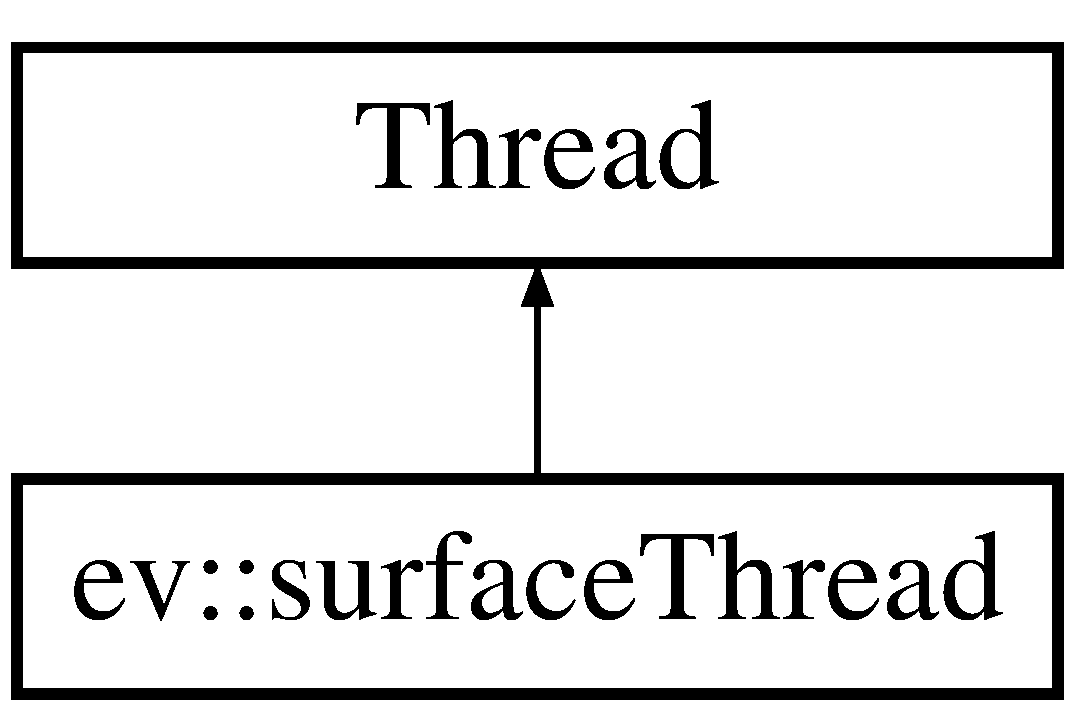
\includegraphics[height=2.000000cm]{classev_1_1surfaceThread}
\end{center}
\end{figure}
\subsection*{Public Member Functions}
\begin{DoxyCompactItemize}
\item 
void {\bfseries configure} (int height, int width)\hypertarget{classev_1_1surfaceThread_a17d8e5af5b6617d91631fe3565e7ec21}{}\label{classev_1_1surfaceThread_a17d8e5af5b6617d91631fe3565e7ec21}

\item 
bool {\bfseries open} (std\+::string portname)\hypertarget{classev_1_1surfaceThread_a8fbb7a7f67aeb8766ee1d222550306c9}{}\label{classev_1_1surfaceThread_a8fbb7a7f67aeb8766ee1d222550306c9}

\item 
void {\bfseries on\+Stop} ()\hypertarget{classev_1_1surfaceThread_a65d324c3c3d8f699412f4fa1eb5aff62}{}\label{classev_1_1surfaceThread_a65d324c3c3d8f699412f4fa1eb5aff62}

\item 
void {\bfseries run} ()\hypertarget{classev_1_1surfaceThread_a04b53ae45896e77a84db501ddfc956cf}{}\label{classev_1_1surfaceThread_a04b53ae45896e77a84db501ddfc956cf}

\item 
yarp\+::os\+::\+Stamp {\bfseries query\+R\+OI} (ev\+::v\+Queue \&fillq, int c, unsigned int t, int x, int y, int r)\hypertarget{classev_1_1surfaceThread_a04b8a2e62c4910346bdfc2ae9c82371b}{}\label{classev_1_1surfaceThread_a04b8a2e62c4910346bdfc2ae9c82371b}

\item 
yarp\+::os\+::\+Stamp {\bfseries query\+Window} (ev\+::v\+Queue \&fillq, int c, unsigned int t)\hypertarget{classev_1_1surfaceThread_ad552b309bca76006c5e8adc07fdcbb6a}{}\label{classev_1_1surfaceThread_ad552b309bca76006c5e8adc07fdcbb6a}

\item 
unsigned int {\bfseries query\+V\+Time} ()\hypertarget{classev_1_1surfaceThread_a763bb2d669fdc772316f074fd43c82d8}{}\label{classev_1_1surfaceThread_a763bb2d669fdc772316f074fd43c82d8}

\end{DoxyCompactItemize}


\subsection{Detailed Description}
asynchronously read events and push them in a \hyperlink{classev_1_1vSurface}{v\+Surface} 

The documentation for this class was generated from the following file\+:\begin{DoxyCompactItemize}
\item 
/home/aglover/workspace/projects/event-\/driven/libraries/include/i\+Cub/eventdriven/v\+Surface\+Handler\+Th.\+h\end{DoxyCompactItemize}

\hypertarget{classev_1_1syncvstreams}{}\section{ev\+:\+:syncvstreams Class Reference}
\label{classev_1_1syncvstreams}\index{ev\+::syncvstreams@{ev\+::syncvstreams}}


automatically accept multiple event types from different ports (e.\+g. as in the v\+Framer)  




{\ttfamily \#include $<$v\+Surface\+Handler\+Th.\+h$>$}

\subsection*{Public Member Functions}
\begin{DoxyCompactItemize}
\item 
bool {\bfseries open} (std\+::string module\+Name, std\+::string event\+Type)\hypertarget{classev_1_1syncvstreams_acc652540f64e92a0528e25932ff51d8f}{}\label{classev_1_1syncvstreams_acc652540f64e92a0528e25932ff51d8f}

\item 
v\+Queue {\bfseries query\+Window} (std\+::string v\+Type, int channel)\hypertarget{classev_1_1syncvstreams_a347bea90f23cf334667bb3e4b7bcf7a0}{}\label{classev_1_1syncvstreams_a347bea90f23cf334667bb3e4b7bcf7a0}

\item 
void {\bfseries close} ()\hypertarget{classev_1_1syncvstreams_ae4bdb73e97024c7399d8a105bdc8425a}{}\label{classev_1_1syncvstreams_ae4bdb73e97024c7399d8a105bdc8425a}

\item 
yarp\+::os\+::\+Stamp {\bfseries getystamp} ()\hypertarget{classev_1_1syncvstreams_a61e65f054ee803198d3e642df2bc1024}{}\label{classev_1_1syncvstreams_a61e65f054ee803198d3e642df2bc1024}

\item 
int {\bfseries getvstamp} ()\hypertarget{classev_1_1syncvstreams_a8846f86bb2794a7b6117c4f9d9c9fa65}{}\label{classev_1_1syncvstreams_a8846f86bb2794a7b6117c4f9d9c9fa65}

\end{DoxyCompactItemize}


\subsection{Detailed Description}
automatically accept multiple event types from different ports (e.\+g. as in the v\+Framer) 

The documentation for this class was generated from the following file\+:\begin{DoxyCompactItemize}
\item 
/home/aglover/workspace/projects/event-\/driven/libraries/include/i\+Cub/eventdriven/v\+Surface\+Handler\+Th.\+h\end{DoxyCompactItemize}

\hypertarget{classev_1_1temporalSurface}{}\section{ev\+:\+:temporal\+Surface Class Reference}
\label{classev_1_1temporalSurface}\index{ev\+::temporal\+Surface@{ev\+::temporal\+Surface}}


a spatio-\/temporal surface storing events for a limited time  




{\ttfamily \#include $<$v\+Window\+\_\+adv.\+h$>$}

Inheritance diagram for ev\+:\+:temporal\+Surface\+:\begin{figure}[H]
\begin{center}
\leavevmode
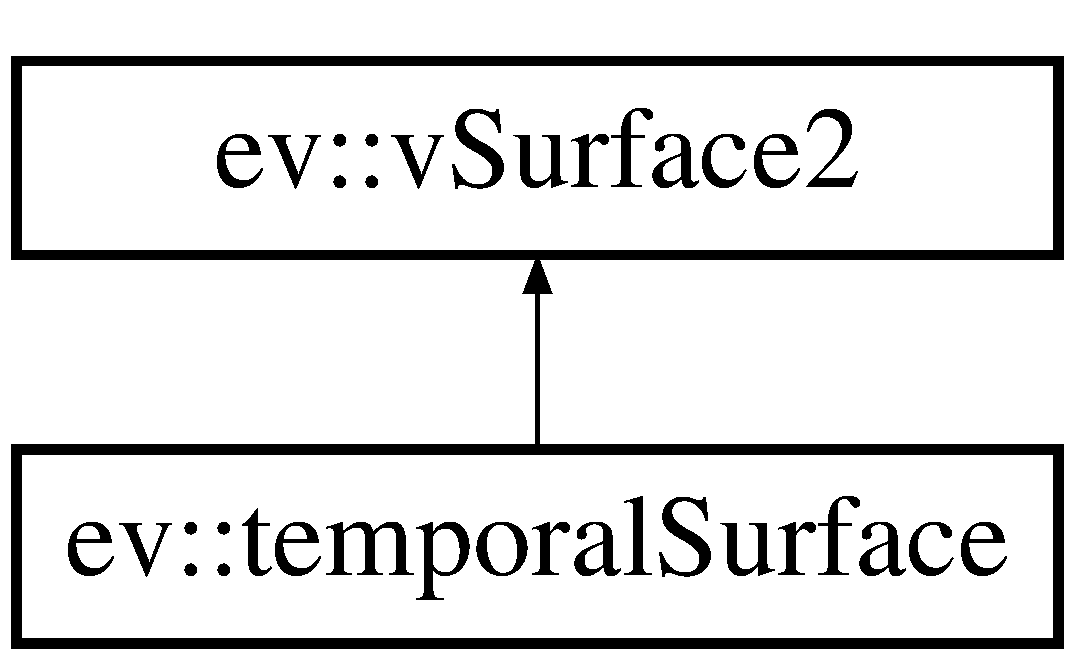
\includegraphics[height=2.000000cm]{classev_1_1temporalSurface}
\end{center}
\end{figure}
\subsection*{Public Member Functions}
\begin{DoxyCompactItemize}
\item 
{\bfseries temporal\+Surface} (int \hyperlink{classev_1_1vSurface2_a1aa8027816352a15d5b9bf1f26f48e76}{width}=128, int height=128, int duration=vts\+Helper\+::max\+Stamp()$\ast$0.\+5)\hypertarget{classev_1_1temporalSurface_ad2f8ebcbe5ff5825d0473cd05f00389e}{}\label{classev_1_1temporalSurface_ad2f8ebcbe5ff5825d0473cd05f00389e}

\item 
virtual v\+Queue {\bfseries remove\+Events} (event$<$$>$ to\+Add)\hypertarget{classev_1_1temporalSurface_a358c548e6727aa89d908e61ad948b1ca}{}\label{classev_1_1temporalSurface_a358c548e6727aa89d908e61ad948b1ca}

\item 
virtual void {\bfseries fast\+Remove\+Events} (event$<$$>$ to\+Add)\hypertarget{classev_1_1temporalSurface_a78a9bb93145915a90a5105bab812bb65}{}\label{classev_1_1temporalSurface_a78a9bb93145915a90a5105bab812bb65}

\item 
void {\bfseries set\+Temporal\+Size} (int duration)\hypertarget{classev_1_1temporalSurface_a35d4b67c18393961fa833d330a040e80}{}\label{classev_1_1temporalSurface_a35d4b67c18393961fa833d330a040e80}

\end{DoxyCompactItemize}
\subsection*{Additional Inherited Members}


\subsection{Detailed Description}
a spatio-\/temporal surface storing events for a limited time 

The documentation for this class was generated from the following files\+:\begin{DoxyCompactItemize}
\item 
/home/aglover/workspace/projects/event-\/driven/libraries/include/i\+Cub/eventdriven/v\+Window\+\_\+adv.\+h\item 
/home/aglover/workspace/projects/event-\/driven/libraries/src/v\+Window\+\_\+adv.\+cpp\end{DoxyCompactItemize}

\hypertarget{classTrackerPool}{}\section{Tracker\+Pool Class Reference}
\label{classTrackerPool}\index{Tracker\+Pool@{Tracker\+Pool}}
\subsection*{Public Member Functions}
\begin{DoxyCompactItemize}
\item 
void {\bfseries set\+Initial\+Params} (double sig\+\_\+x, double sig\+\_\+y, double sig\+\_\+xy, double alpha\+\_\+pos, double alpha\+\_\+shape, bool fixed\+\_\+shape)\hypertarget{classTrackerPool_aba64099a18fc9b97eeb5b60f92ca849c}{}\label{classTrackerPool_aba64099a18fc9b97eeb5b60f92ca849c}

\item 
void {\bfseries set\+Decay\+Params} (double decay\+\_\+tau, double Tact, double Tinact, double Tfree, double Tevent, int rate)\hypertarget{classTrackerPool_aacfd7b8d8f8d47cf609e6e4ed64bbc1a}{}\label{classTrackerPool_aacfd7b8d8f8d47cf609e6e4ed64bbc1a}

\item 
void {\bfseries set\+Comparison\+Params} (double max\+\_\+dist)\hypertarget{classTrackerPool_a2ae5849c22bc24b688bd5ddf153e9e33}{}\label{classTrackerPool_a2ae5849c22bc24b688bd5ddf153e9e33}

\item 
void {\bfseries set\+Cluster\+Limit} (int limit)\hypertarget{classTrackerPool_a947f58bef9d46a290cb3ea6ec99d5fb8}{}\label{classTrackerPool_a947f58bef9d46a290cb3ea6ec99d5fb8}

\item 
int {\bfseries update} (ev\+::event$<$ \hyperlink{classev_1_1AddressEvent}{ev\+::\+Address\+Event} $>$ v, std\+::vector$<$ ev\+::event$<$ \hyperlink{classev_1_1GaussianAE}{ev\+::\+Gaussian\+AE} $>$ $>$ \&cl\+Evts)\hypertarget{classTrackerPool_a07051233ee59f248fbed73f3e8819e96}{}\label{classTrackerPool_a07051233ee59f248fbed73f3e8819e96}

\end{DoxyCompactItemize}
\subsection*{Protected Member Functions}
\begin{DoxyCompactItemize}
\item 
int {\bfseries get\+New\+Tracker} ()\hypertarget{classTrackerPool_afc17f68023420c6d43ac4b67afa3b14d}{}\label{classTrackerPool_afc17f68023420c6d43ac4b67afa3b14d}

\item 
ev\+::event$<$ \hyperlink{classev_1_1GaussianAE}{ev\+::\+Gaussian\+AE} $>$ {\bfseries make\+Event} (int i, int ts)\hypertarget{classTrackerPool_afc0696873f8071a97bdfeca16580d132}{}\label{classTrackerPool_afc0696873f8071a97bdfeca16580d132}

\end{DoxyCompactItemize}
\subsection*{Protected Attributes}
\begin{DoxyCompactItemize}
\item 
std\+::vector$<$ \hyperlink{classBlobTracker}{Blob\+Tracker} $>$ {\bfseries trackers\+\_\+}\hypertarget{classTrackerPool_a8a8bdb245a4e706de8f9263cc31537cd}{}\label{classTrackerPool_a8a8bdb245a4e706de8f9263cc31537cd}

\item 
int {\bfseries nb\+\_\+ev\+\_\+regulate\+\_\+}\hypertarget{classTrackerPool_af542ddb16630e451065d5e3258cd19de}{}\label{classTrackerPool_af542ddb16630e451065d5e3258cd19de}

\item 
int {\bfseries count\+\_\+}\hypertarget{classTrackerPool_a5aed0a9c9621c9fde35034a8b5f58085}{}\label{classTrackerPool_a5aed0a9c9621c9fde35034a8b5f58085}

\item 
unsigned long int {\bfseries ts\+\_\+last\+\_\+reg\+\_\+}\hypertarget{classTrackerPool_ac8ecd306ab6f0562ca2d6231ff367093}{}\label{classTrackerPool_ac8ecd306ab6f0562ca2d6231ff367093}

\item 
double {\bfseries decay\+\_\+tau}\hypertarget{classTrackerPool_abe7439ab3a403e77b56def1ae14ef1c3}{}\label{classTrackerPool_abe7439ab3a403e77b56def1ae14ef1c3}

\item 
double {\bfseries Tact}\hypertarget{classTrackerPool_aaf7de0a0903e66d7ae07cc11cb6ea072}{}\label{classTrackerPool_aaf7de0a0903e66d7ae07cc11cb6ea072}

\item 
double {\bfseries Tinact}\hypertarget{classTrackerPool_a75d2a1d3867ac839d3c24aa26241950e}{}\label{classTrackerPool_a75d2a1d3867ac839d3c24aa26241950e}

\item 
double {\bfseries Tfree}\hypertarget{classTrackerPool_ac75f2360d9bb76e0a6c79b31129c58c5}{}\label{classTrackerPool_ac75f2360d9bb76e0a6c79b31129c58c5}

\item 
double {\bfseries Tevent}\hypertarget{classTrackerPool_a3798b118a9592e75d59ad0d0e5fe438b}{}\label{classTrackerPool_a3798b118a9592e75d59ad0d0e5fe438b}

\item 
double {\bfseries max\+\_\+dist}\hypertarget{classTrackerPool_ad57d26c00d4329747f59df1b7b24ea3b}{}\label{classTrackerPool_ad57d26c00d4329747f59df1b7b24ea3b}

\item 
bool {\bfseries fixed\+\_\+shape\+\_\+}\hypertarget{classTrackerPool_af83ad39640f58a747253b85046083140}{}\label{classTrackerPool_af83ad39640f58a747253b85046083140}

\item 
double {\bfseries sig\+\_\+x2\+\_\+}\hypertarget{classTrackerPool_a6a92ea09387253159839324143b6206a}{}\label{classTrackerPool_a6a92ea09387253159839324143b6206a}

\item 
double {\bfseries sig\+\_\+y2\+\_\+}\hypertarget{classTrackerPool_a3181cb8343949ab80181c9028ae114fa}{}\label{classTrackerPool_a3181cb8343949ab80181c9028ae114fa}

\item 
double {\bfseries sig\+\_\+xy\+\_\+}\hypertarget{classTrackerPool_a9018c85457b2616efe8f718f1602b32a}{}\label{classTrackerPool_a9018c85457b2616efe8f718f1602b32a}

\item 
double {\bfseries alpha\+\_\+pos}\hypertarget{classTrackerPool_ad67aaae3b2c777330ccb4abb9bf60884}{}\label{classTrackerPool_ad67aaae3b2c777330ccb4abb9bf60884}

\item 
double {\bfseries alpha\+\_\+shape}\hypertarget{classTrackerPool_ad134dda445a2b5eea2d2101a6e5c2132}{}\label{classTrackerPool_ad134dda445a2b5eea2d2101a6e5c2132}

\item 
double {\bfseries cluster\+Limit}\hypertarget{classTrackerPool_a6c9e6cdff31c0ab40c19f54d30d315cc}{}\label{classTrackerPool_a6c9e6cdff31c0ab40c19f54d30d315cc}

\item 
\hyperlink{classev_1_1vtsHelper}{ev\+::vts\+Helper} {\bfseries unwrap}\hypertarget{classTrackerPool_afec5b627c70b35454cecd812b3913c59}{}\label{classTrackerPool_afec5b627c70b35454cecd812b3913c59}

\end{DoxyCompactItemize}


The documentation for this class was generated from the following files\+:\begin{DoxyCompactItemize}
\item 
/home/aglover/workspace/projects/event-\/driven/src/processing/v\+Cluster/include/tracker\+Pool.\+h\item 
/home/aglover/workspace/projects/event-\/driven/src/processing/v\+Cluster/src/tracker\+Pool.\+cpp\end{DoxyCompactItemize}

\hypertarget{classev_1_1tWinThread}{}\section{ev\+:\+:t\+Win\+Thread Class Reference}
\label{classev_1_1tWinThread}\index{ev\+::t\+Win\+Thread@{ev\+::t\+Win\+Thread}}


automatically accept events from a port and push them into a \hyperlink{classev_1_1vTempWindow}{v\+Temp\+Window}  




{\ttfamily \#include $<$v\+Surface\+Handler\+Th.\+h$>$}

Inheritance diagram for ev\+:\+:t\+Win\+Thread\+:\begin{figure}[H]
\begin{center}
\leavevmode
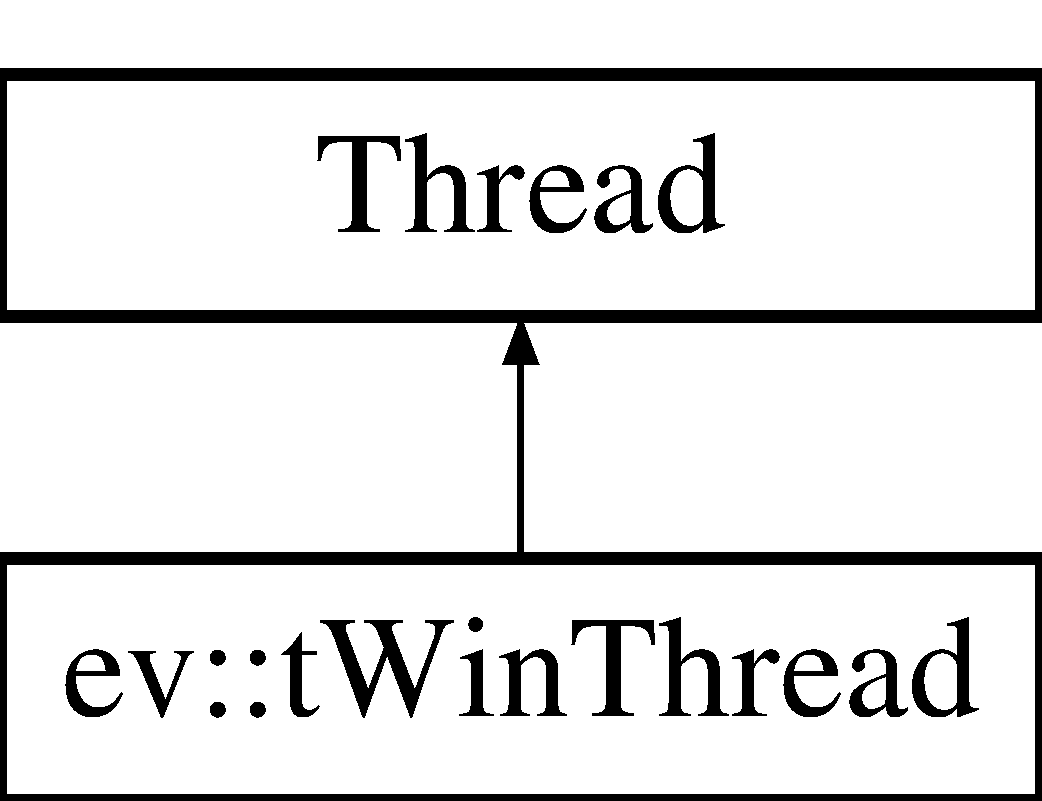
\includegraphics[height=2.000000cm]{classev_1_1tWinThread}
\end{center}
\end{figure}
\subsection*{Public Member Functions}
\begin{DoxyCompactItemize}
\item 
bool {\bfseries open} (std\+::string portname)\hypertarget{classev_1_1tWinThread_a38015410daeb0a64cf458a5d996192b3}{}\label{classev_1_1tWinThread_a38015410daeb0a64cf458a5d996192b3}

\item 
void {\bfseries on\+Stop} ()\hypertarget{classev_1_1tWinThread_ab12b04cd804ac7f6d2f6a199bb2078a8}{}\label{classev_1_1tWinThread_ab12b04cd804ac7f6d2f6a199bb2078a8}

\item 
void {\bfseries run} ()\hypertarget{classev_1_1tWinThread_a6992dcf7884d08d7296e4489ef264959}{}\label{classev_1_1tWinThread_a6992dcf7884d08d7296e4489ef264959}

\item 
v\+Queue {\bfseries query\+Window} (int channel)\hypertarget{classev_1_1tWinThread_a6937e3d587982b4ecbc8e776c89b5ea1}{}\label{classev_1_1tWinThread_a6937e3d587982b4ecbc8e776c89b5ea1}

\item 
void {\bfseries query\+Stamps} (yarp\+::os\+::\+Stamp \&y\+Stamp, int \&v\+Stamp)\hypertarget{classev_1_1tWinThread_a346e943bc1a1e06210deb6da26fa18f6}{}\label{classev_1_1tWinThread_a346e943bc1a1e06210deb6da26fa18f6}

\end{DoxyCompactItemize}


\subsection{Detailed Description}
automatically accept events from a port and push them into a \hyperlink{classev_1_1vTempWindow}{v\+Temp\+Window} 

The documentation for this class was generated from the following file\+:\begin{DoxyCompactItemize}
\item 
/home/aglover/workspace/projects/event-\/driven/libraries/include/i\+Cub/eventdriven/v\+Surface\+Handler\+Th.\+h\end{DoxyCompactItemize}

\hypertarget{classev_1_1vBottle}{}\section{ev\+:\+:v\+Bottle Class Reference}
\label{classev_1_1vBottle}\index{ev\+::v\+Bottle@{ev\+::v\+Bottle}}


yarp\+::os\+::\+Bottle wrapper for sending events through the yarp system with particular attention to using data dumper and data players  




{\ttfamily \#include $<$v\+Bottle.\+h$>$}

Inheritance diagram for ev\+:\+:v\+Bottle\+:\begin{figure}[H]
\begin{center}
\leavevmode
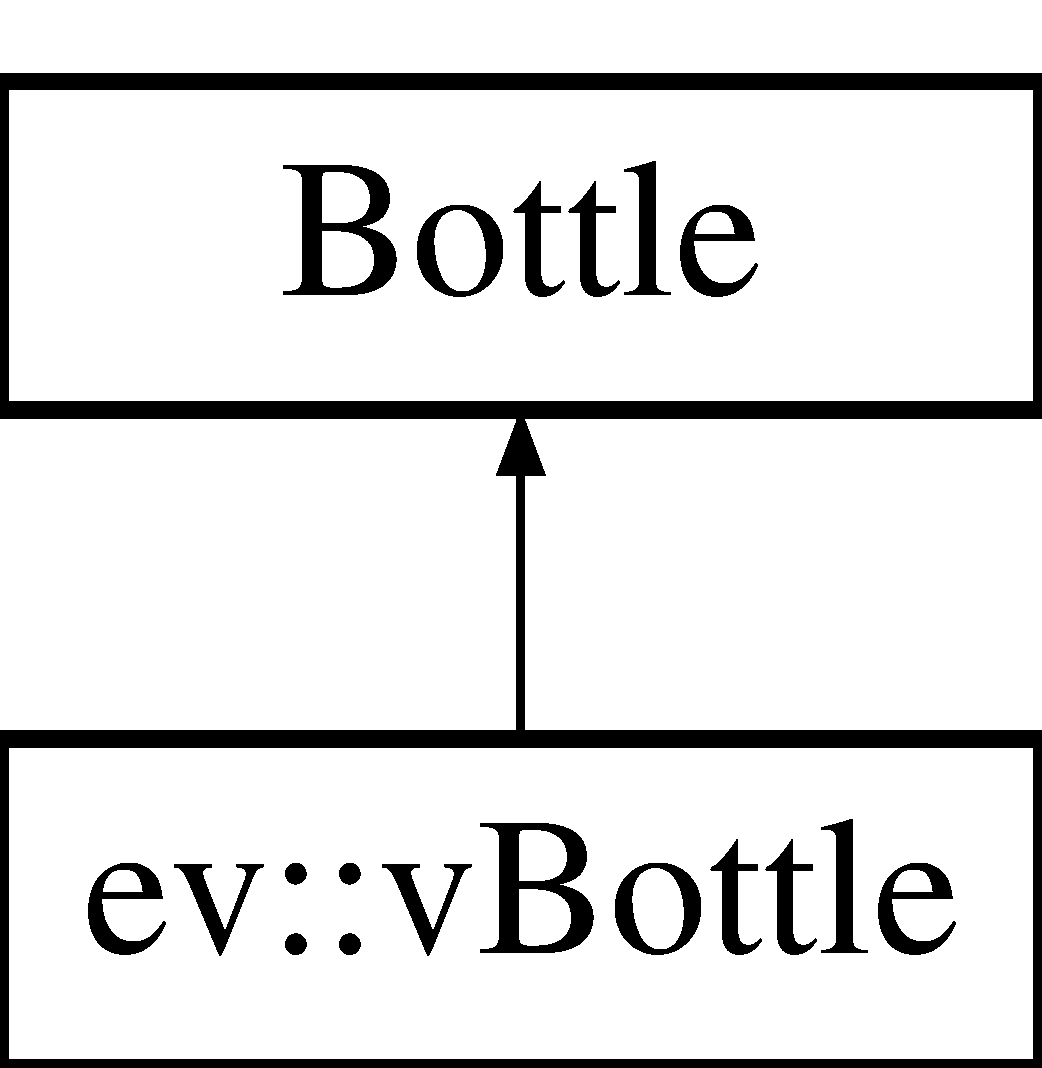
\includegraphics[height=2.000000cm]{classev_1_1vBottle}
\end{center}
\end{figure}
\subsection*{Public Member Functions}
\begin{DoxyCompactItemize}
\item 
void {\bfseries add\+Event} (event$<$$>$ e)\hypertarget{classev_1_1vBottle_a5b17f0b46d9260ab255f38382b4b7268}{}\label{classev_1_1vBottle_a5b17f0b46d9260ab255f38382b4b7268}

\item 
void {\bfseries append} (\hyperlink{classev_1_1vBottle}{v\+Bottle} \&eb)\hypertarget{classev_1_1vBottle_a0c78e6f9ef839038d71486f6a8a6294a}{}\label{classev_1_1vBottle_a0c78e6f9ef839038d71486f6a8a6294a}

\item 
{\footnotesize template$<$class T $>$ }\\void {\bfseries append} (\hyperlink{classev_1_1vBottle}{v\+Bottle} \&eb)\hypertarget{classev_1_1vBottle_a9ef66f613e1bbf196c515e7d8b0416df}{}\label{classev_1_1vBottle_a9ef66f613e1bbf196c515e7d8b0416df}

\item 
{\footnotesize template$<$class T $>$ }\\v\+Queue {\bfseries get} ()\hypertarget{classev_1_1vBottle_a86302277c279a1b02d92f8e12afe6a2c}{}\label{classev_1_1vBottle_a86302277c279a1b02d92f8e12afe6a2c}

\item 
{\footnotesize template$<$class T $>$ }\\void {\bfseries addtoendof} (v\+Queue \&q)\hypertarget{classev_1_1vBottle_a65bf90aec03b80dee45bf834efe3fbfc}{}\label{classev_1_1vBottle_a65bf90aec03b80dee45bf834efe3fbfc}

\item 
{\footnotesize template$<$class T $>$ }\\v\+Queue {\bfseries get\+Sorted} ()\hypertarget{classev_1_1vBottle_a27569b9aaa7eb1ff9135d435b841c2de}{}\label{classev_1_1vBottle_a27569b9aaa7eb1ff9135d435b841c2de}

\item 
v\+Queue {\bfseries get\+All} ()\hypertarget{classev_1_1vBottle_af2abadf41f73c455dd451e34e9ba3376}{}\label{classev_1_1vBottle_af2abadf41f73c455dd451e34e9ba3376}

\item 
v\+Queue {\bfseries get\+All\+Sorted} ()\hypertarget{classev_1_1vBottle_a273cfda65fed58bcf19cedf6652948d9}{}\label{classev_1_1vBottle_a273cfda65fed58bcf19cedf6652948d9}

\end{DoxyCompactItemize}


\subsection{Detailed Description}
yarp\+::os\+::\+Bottle wrapper for sending events through the yarp system with particular attention to using data dumper and data players 

The documentation for this class was generated from the following file\+:\begin{DoxyCompactItemize}
\item 
/home/aglover/workspace/projects/event-\/driven/libraries/include/i\+Cub/eventdriven/v\+Bottle.\+h\end{DoxyCompactItemize}

\hypertarget{classev_1_1vBottleMimic}{}\section{ev\+:\+:v\+Bottle\+Mimic Class Reference}
\label{classev_1_1vBottleMimic}\index{ev\+::v\+Bottle\+Mimic@{ev\+::v\+Bottle\+Mimic}}


add header data to a block of data to correctly send it as a \hyperlink{classev_1_1vBottle}{v\+Bottle} without copying data  




{\ttfamily \#include $<$v\+Bottle.\+h$>$}

Inheritance diagram for ev\+:\+:v\+Bottle\+Mimic\+:\begin{figure}[H]
\begin{center}
\leavevmode
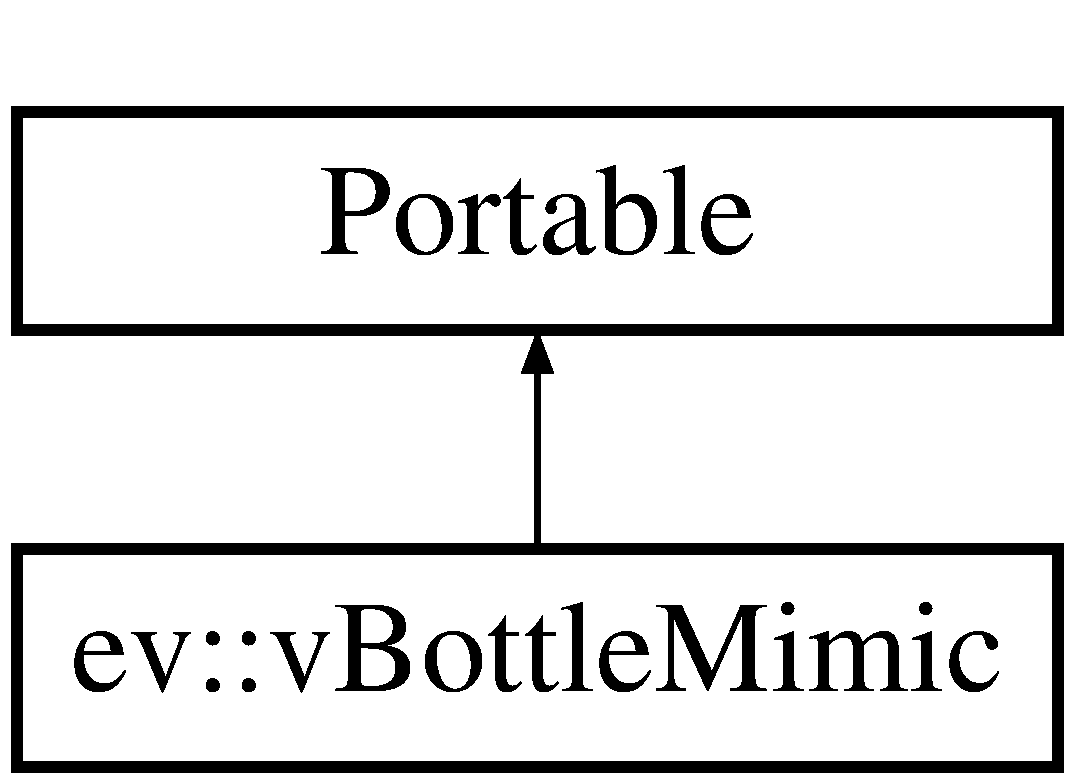
\includegraphics[height=2.000000cm]{classev_1_1vBottleMimic}
\end{center}
\end{figure}
\subsection*{Public Member Functions}
\begin{DoxyCompactItemize}
\item 
void {\bfseries setdata} (const char $\ast$datablock, unsigned int datalength)\hypertarget{classev_1_1vBottleMimic_a03c64a63225e333a11b2693213f44165}{}\label{classev_1_1vBottleMimic_a03c64a63225e333a11b2693213f44165}

\item 
virtual bool {\bfseries read} (yarp\+::os\+::\+Connection\+Reader \&connection)\hypertarget{classev_1_1vBottleMimic_a5c7ead7b0484b9abe99e922196c074ff}{}\label{classev_1_1vBottleMimic_a5c7ead7b0484b9abe99e922196c074ff}

\item 
virtual bool {\bfseries write} (yarp\+::os\+::\+Connection\+Writer \&connection)\hypertarget{classev_1_1vBottleMimic_a39ad9b924890d8f8f717f49b6c5ad23f}{}\label{classev_1_1vBottleMimic_a39ad9b924890d8f8f717f49b6c5ad23f}

\end{DoxyCompactItemize}


\subsection{Detailed Description}
add header data to a block of data to correctly send it as a \hyperlink{classev_1_1vBottle}{v\+Bottle} without copying data 

The documentation for this class was generated from the following file\+:\begin{DoxyCompactItemize}
\item 
/home/aglover/workspace/projects/event-\/driven/libraries/include/i\+Cub/eventdriven/v\+Bottle.\+h\end{DoxyCompactItemize}

\hypertarget{classvCircleModule}{}\section{v\+Circle\+Module Class Reference}
\label{classvCircleModule}\index{v\+Circle\+Module@{v\+Circle\+Module}}
Inheritance diagram for v\+Circle\+Module\+:\begin{figure}[H]
\begin{center}
\leavevmode
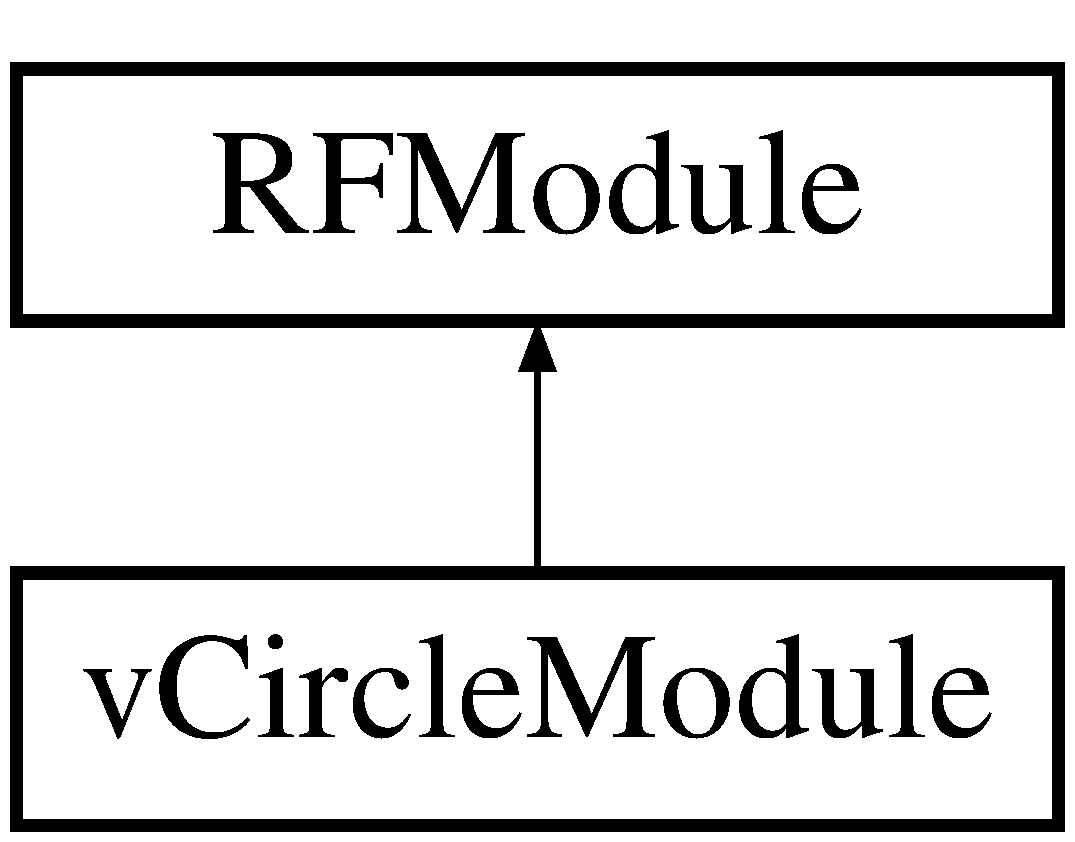
\includegraphics[height=2.000000cm]{classvCircleModule}
\end{center}
\end{figure}
\subsection*{Public Member Functions}
\begin{DoxyCompactItemize}
\item 
virtual bool {\bfseries configure} (yarp\+::os\+::\+Resource\+Finder \&rf)\hypertarget{classvCircleModule_a4b1534c8acd2a20a874b1e3fb2f2bbbf}{}\label{classvCircleModule_a4b1534c8acd2a20a874b1e3fb2f2bbbf}

\item 
virtual bool {\bfseries interrupt\+Module} ()\hypertarget{classvCircleModule_aee48b945926e1ee1d53c03d2f8fdb462}{}\label{classvCircleModule_aee48b945926e1ee1d53c03d2f8fdb462}

\item 
virtual bool {\bfseries close} ()\hypertarget{classvCircleModule_a9c266baf21bf1a84e1d47bc82a6ebbaa}{}\label{classvCircleModule_a9c266baf21bf1a84e1d47bc82a6ebbaa}

\item 
virtual double {\bfseries get\+Period} ()\hypertarget{classvCircleModule_a87f95035935e336eef6b9890920c1bcb}{}\label{classvCircleModule_a87f95035935e336eef6b9890920c1bcb}

\item 
virtual bool {\bfseries update\+Module} ()\hypertarget{classvCircleModule_a0137387e1760f41bb422e10c702df2a0}{}\label{classvCircleModule_a0137387e1760f41bb422e10c702df2a0}

\end{DoxyCompactItemize}


The documentation for this class was generated from the following files\+:\begin{DoxyCompactItemize}
\item 
/home/aglover/workspace/projects/event-\/driven/src/processing/v\+Circle/include/v\+Circle\+Module.\+h\item 
/home/aglover/workspace/projects/event-\/driven/src/processing/v\+Circle/src/v\+Circle\+Module.\+cpp\end{DoxyCompactItemize}

\hypertarget{classvCircleMultiSize}{}\section{v\+Circle\+Multi\+Size Class Reference}
\label{classvCircleMultiSize}\index{v\+Circle\+Multi\+Size@{v\+Circle\+Multi\+Size}}
\subsection*{Public Member Functions}
\begin{DoxyCompactItemize}
\item 
{\bfseries v\+Circle\+Multi\+Size} (double threshold, std\+::string q\+Type=\char`\"{}edge\char`\"{}, int r\+Low=8, int r\+High=38, bool directed=true, bool parallel=false, int height=128, int width=128, int arclength=20, double fifolength=2000)\hypertarget{classvCircleMultiSize_aa3e7373ef68728fab536417c491e35a4}{}\label{classvCircleMultiSize_aa3e7373ef68728fab536417c491e35a4}

\item 
void {\bfseries set\+Channel} (int channel\+Number)\hypertarget{classvCircleMultiSize_afe4c5983834ed7d5fa097fcc9677d234}{}\label{classvCircleMultiSize_afe4c5983834ed7d5fa097fcc9677d234}

\item 
void {\bfseries add\+Queue} (ev\+::v\+Queue \&additions)\hypertarget{classvCircleMultiSize_a101a1960c5012a83e03b9fdd8276f263}{}\label{classvCircleMultiSize_a101a1960c5012a83e03b9fdd8276f263}

\item 
double {\bfseries get\+Obs} (int \&x, int \&y, int \&r)\hypertarget{classvCircleMultiSize_a661f425152259951f87167bdcd53caaf}{}\label{classvCircleMultiSize_a661f425152259951f87167bdcd53caaf}

\item 
std\+::vector$<$ double $>$ {\bfseries get\+Percentile} (double p, double th\+Min)\hypertarget{classvCircleMultiSize_a92b94e14acce928e07922809a45cd5c0}{}\label{classvCircleMultiSize_a92b94e14acce928e07922809a45cd5c0}

\item 
yarp\+::sig\+::\+Image\+Of$<$ yarp\+::sig\+::\+Pixel\+Bgr $>$ {\bfseries make\+Debug\+Image} ()\hypertarget{classvCircleMultiSize_a1dc2c81da6abc8aaaaedf0d169ad9671}{}\label{classvCircleMultiSize_a1dc2c81da6abc8aaaaedf0d169ad9671}

\end{DoxyCompactItemize}


The documentation for this class was generated from the following files\+:\begin{DoxyCompactItemize}
\item 
/home/aglover/workspace/projects/event-\/driven/src/processing/v\+Circle/include/v\+Circle\+Observer.\+h\item 
/home/aglover/workspace/projects/event-\/driven/src/processing/v\+Circle/src/v\+Circle\+Observer.\+cpp\end{DoxyCompactItemize}

\hypertarget{classvCircleReader}{}\section{v\+Circle\+Reader Class Reference}
\label{classvCircleReader}\index{v\+Circle\+Reader@{v\+Circle\+Reader}}
Inheritance diagram for v\+Circle\+Reader\+:\begin{figure}[H]
\begin{center}
\leavevmode
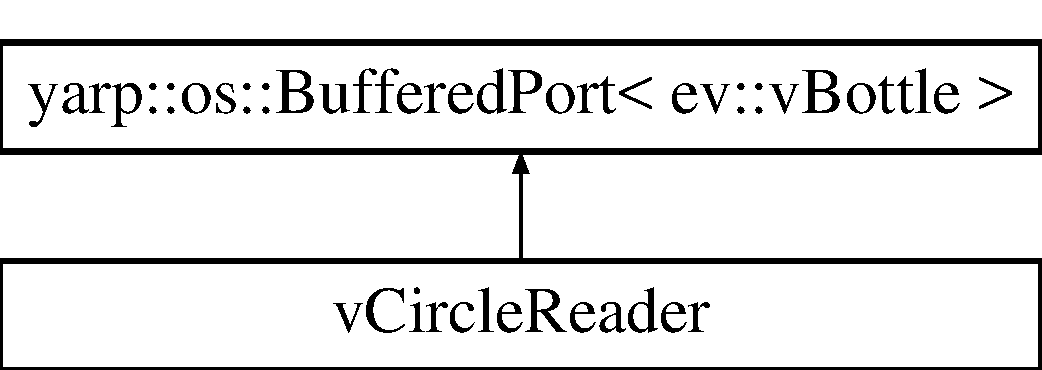
\includegraphics[height=2.000000cm]{classvCircleReader}
\end{center}
\end{figure}
\subsection*{Public Member Functions}
\begin{DoxyCompactItemize}
\item 
void {\bfseries set\+SingleQ} (bool singleq=true)\hypertarget{classvCircleReader_a35b57eb759bf78b3199e2b058f509b19}{}\label{classvCircleReader_a35b57eb759bf78b3199e2b058f509b19}

\item 
bool {\bfseries open} (const std\+::string \&name, bool strictness=false)\hypertarget{classvCircleReader_aeea09b1b0a4f6ca43362430e2b7c13f3}{}\label{classvCircleReader_aeea09b1b0a4f6ca43362430e2b7c13f3}

\item 
void {\bfseries close} ()\hypertarget{classvCircleReader_a963ecb3d9e66c9a6d0dd3deb0107d333}{}\label{classvCircleReader_a963ecb3d9e66c9a6d0dd3deb0107d333}

\item 
void {\bfseries interrupt} ()\hypertarget{classvCircleReader_adb1e49808d1ff24b38e68ad3c706d87a}{}\label{classvCircleReader_adb1e49808d1ff24b38e68ad3c706d87a}

\item 
void {\bfseries on\+Read} (\hyperlink{classev_1_1vBottle}{ev\+::v\+Bottle} \&in\+Bot)\hypertarget{classvCircleReader_ae0f761bdd9af2bae8edc2e0f2766ff39}{}\label{classvCircleReader_ae0f761bdd9af2bae8edc2e0f2766ff39}

\end{DoxyCompactItemize}
\subsection*{Public Attributes}
\begin{DoxyCompactItemize}
\item 
\hyperlink{classvCircleMultiSize}{v\+Circle\+Multi\+Size} $\ast$ {\bfseries c\+ObserverL}\hypertarget{classvCircleReader_a75c47ee3024729fab391fc0098147430}{}\label{classvCircleReader_a75c47ee3024729fab391fc0098147430}

\item 
\hyperlink{classvCircleMultiSize}{v\+Circle\+Multi\+Size} $\ast$ {\bfseries c\+ObserverR}\hypertarget{classvCircleReader_a52940184b5d5f348813fdfdf1a62da48}{}\label{classvCircleReader_a52940184b5d5f348813fdfdf1a62da48}

\item 
double {\bfseries inlier\+Threshold}\hypertarget{classvCircleReader_abb1da4c345eb519b695927d12f2f1ec8}{}\label{classvCircleReader_abb1da4c345eb519b695927d12f2f1ec8}

\item 
bool {\bfseries hough}\hypertarget{classvCircleReader_a2a026b4c43ab7e721b6089b4118767a4}{}\label{classvCircleReader_a2a026b4c43ab7e721b6089b4118767a4}

\item 
double {\bfseries timecounter}\hypertarget{classvCircleReader_a0bcf9e8b5c28b2ea048ab75c4213023e}{}\label{classvCircleReader_a0bcf9e8b5c28b2ea048ab75c4213023e}

\end{DoxyCompactItemize}


The documentation for this class was generated from the following files\+:\begin{DoxyCompactItemize}
\item 
/home/aglover/workspace/projects/event-\/driven/src/processing/v\+Circle/include/v\+Circle\+Module.\+h\item 
/home/aglover/workspace/projects/event-\/driven/src/processing/v\+Circle/src/v\+Circle\+Module.\+cpp\end{DoxyCompactItemize}

\hypertarget{classvCircleThread}{}\section{v\+Circle\+Thread Class Reference}
\label{classvCircleThread}\index{v\+Circle\+Thread@{v\+Circle\+Thread}}


The \hyperlink{classvCircleThread}{v\+Circle\+Thread} class performs a circular Hough transform.  




{\ttfamily \#include $<$v\+Circle\+Observer.\+h$>$}

Inheritance diagram for v\+Circle\+Thread\+:\begin{figure}[H]
\begin{center}
\leavevmode
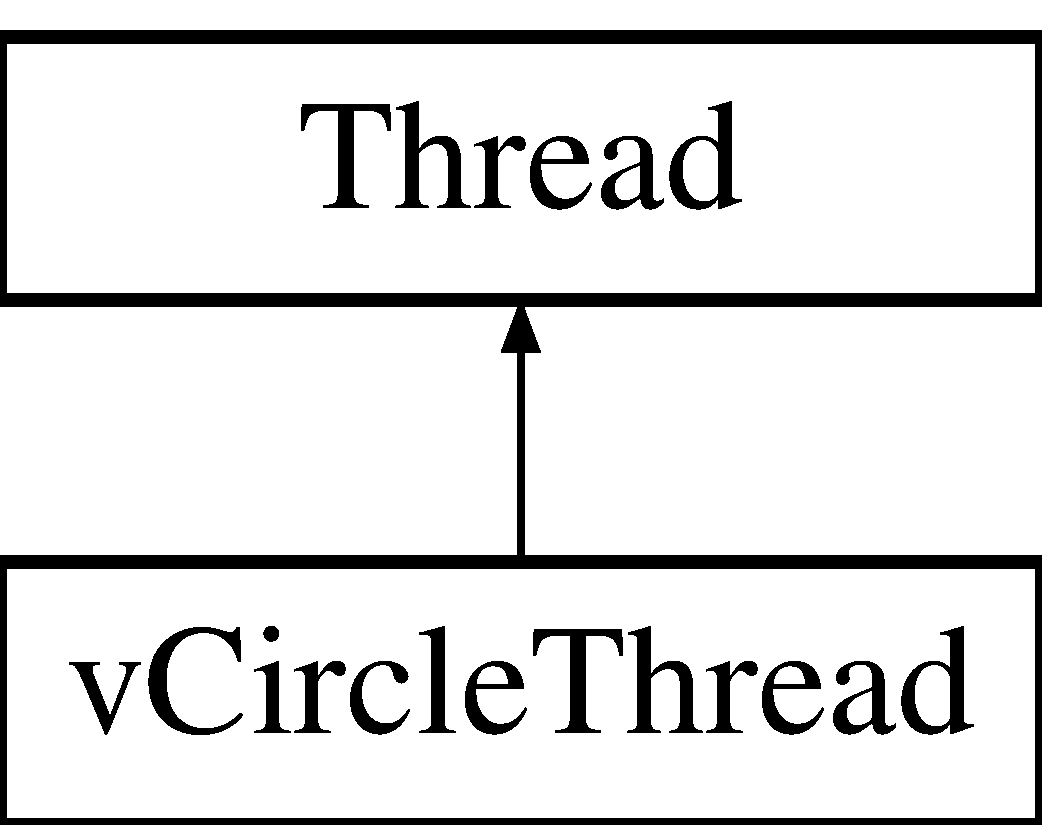
\includegraphics[height=2.000000cm]{classvCircleThread}
\end{center}
\end{figure}
\subsection*{Public Member Functions}
\begin{DoxyCompactItemize}
\item 
\hyperlink{classvCircleThread_adb0ce9432b9fe2a8d853c63b764d7859}{v\+Circle\+Thread} (int R, bool directed, bool parallel=false, int height=128, int width=128, double arclength=15)
\begin{DoxyCompactList}\small\item\em \hyperlink{classvCircleThread}{v\+Circle\+Thread} constructor \end{DoxyCompactList}\item 
double \hyperlink{classvCircleThread_a692a1066ee63c2716998fcb3a7aa513d}{get\+Score} ()
\begin{DoxyCompactList}\small\item\em get\+Score get the maximum strength in Hough space \end{DoxyCompactList}\item 
int \hyperlink{classvCircleThread_a0feac9f937bfeecc2dc0b015f9e8161c}{getX} ()
\begin{DoxyCompactList}\small\item\em getX get the maximum strength location \end{DoxyCompactList}\item 
int \hyperlink{classvCircleThread_a4f39898c53c3178b84b28c8cc33ec352}{getY} ()
\begin{DoxyCompactList}\small\item\em getY get the maximum strength location \end{DoxyCompactList}\item 
int \hyperlink{classvCircleThread_a024aa1ad0a7855fad146425c80feadb0}{getR} ()
\begin{DoxyCompactList}\small\item\em getR return the radius of the circle to be detected \end{DoxyCompactList}\item 
void \hyperlink{classvCircleThread_ad5f114e5609dd616c9eae9d1755d12c1}{process} (ev\+::v\+Queue \&proc\+Queue, std\+::vector$<$ int $>$ \&proc\+Type)
\begin{DoxyCompactList}\small\item\em process update the Hough transform (threaded or non-\/threaded) \end{DoxyCompactList}\item 
void \hyperlink{classvCircleThread_a0d32749f12d2d93ff0d9ccdf37422ccf}{waitfordone} ()\hypertarget{classvCircleThread_a0d32749f12d2d93ff0d9ccdf37422ccf}{}\label{classvCircleThread_a0d32749f12d2d93ff0d9ccdf37422ccf}

\begin{DoxyCompactList}\small\item\em waitfordone wait for computation to finish if threaded \end{DoxyCompactList}\item 
int {\bfseries find\+Scores} (std\+::vector$<$ double $>$ \&values, double threshold)\hypertarget{classvCircleThread_a89b389603f6f6a9395a0381271dee419}{}\label{classvCircleThread_a89b389603f6f6a9395a0381271dee419}

\item 
yarp\+::sig\+::\+Image\+Of$<$ yarp\+::sig\+::\+Pixel\+Bgr $>$ \hyperlink{classvCircleThread_ae19a982e66ba27619a40ecbf128af543}{make\+Debug\+Image} (double refval=-\/1)
\begin{DoxyCompactList}\small\item\em make\+Debug\+Image create an image visualising the Hough space \end{DoxyCompactList}\end{DoxyCompactItemize}


\subsection{Detailed Description}
The \hyperlink{classvCircleThread}{v\+Circle\+Thread} class performs a circular Hough transform. 

The class gives the maximal location and strength of a circular shape of a single given radius. The class can use the directed transform and can be threaded for use on multi-\/core systems. 

\subsection{Constructor \& Destructor Documentation}
\index{v\+Circle\+Thread@{v\+Circle\+Thread}!v\+Circle\+Thread@{v\+Circle\+Thread}}
\index{v\+Circle\+Thread@{v\+Circle\+Thread}!v\+Circle\+Thread@{v\+Circle\+Thread}}
\subsubsection[{\texorpdfstring{v\+Circle\+Thread(int R, bool directed, bool parallel=false, int height=128, int width=128, double arclength=15)}{vCircleThread(int R, bool directed, bool parallel=false, int height=128, int width=128, double arclength=15)}}]{\setlength{\rightskip}{0pt plus 5cm}v\+Circle\+Thread\+::v\+Circle\+Thread (
\begin{DoxyParamCaption}
\item[{int}]{R, }
\item[{bool}]{directed, }
\item[{bool}]{parallel = {\ttfamily false}, }
\item[{int}]{height = {\ttfamily 128}, }
\item[{int}]{width = {\ttfamily 128}, }
\item[{double}]{arclength = {\ttfamily 15}}
\end{DoxyParamCaption}
)}\hypertarget{classvCircleThread_adb0ce9432b9fe2a8d853c63b764d7859}{}\label{classvCircleThread_adb0ce9432b9fe2a8d853c63b764d7859}


\hyperlink{classvCircleThread}{v\+Circle\+Thread} constructor 


\begin{DoxyParams}{Parameters}
{\em R} & circle radius \\
\hline
{\em directed} & use directed Hough transform \\
\hline
{\em parallel} & use a separate thread for computation \\
\hline
{\em height} & sensor height \\
\hline
{\em width} & sensor width \\
\hline
\end{DoxyParams}


\subsection{Member Function Documentation}
\index{v\+Circle\+Thread@{v\+Circle\+Thread}!getR@{getR}}
\index{getR@{getR}!v\+Circle\+Thread@{v\+Circle\+Thread}}
\subsubsection[{\texorpdfstring{get\+R()}{getR()}}]{\setlength{\rightskip}{0pt plus 5cm}int v\+Circle\+Thread\+::getR (
\begin{DoxyParamCaption}
{}
\end{DoxyParamCaption}
)\hspace{0.3cm}{\ttfamily [inline]}}\hypertarget{classvCircleThread_a024aa1ad0a7855fad146425c80feadb0}{}\label{classvCircleThread_a024aa1ad0a7855fad146425c80feadb0}


getR return the radius of the circle to be detected 

\begin{DoxyReturn}{Returns}
the radius R 
\end{DoxyReturn}
\index{v\+Circle\+Thread@{v\+Circle\+Thread}!get\+Score@{get\+Score}}
\index{get\+Score@{get\+Score}!v\+Circle\+Thread@{v\+Circle\+Thread}}
\subsubsection[{\texorpdfstring{get\+Score()}{getScore()}}]{\setlength{\rightskip}{0pt plus 5cm}double v\+Circle\+Thread\+::get\+Score (
\begin{DoxyParamCaption}
{}
\end{DoxyParamCaption}
)\hspace{0.3cm}{\ttfamily [inline]}}\hypertarget{classvCircleThread_a692a1066ee63c2716998fcb3a7aa513d}{}\label{classvCircleThread_a692a1066ee63c2716998fcb3a7aa513d}


get\+Score get the maximum strength in Hough space 

\begin{DoxyReturn}{Returns}
the maximum strength in Hough space 
\end{DoxyReturn}
\index{v\+Circle\+Thread@{v\+Circle\+Thread}!getX@{getX}}
\index{getX@{getX}!v\+Circle\+Thread@{v\+Circle\+Thread}}
\subsubsection[{\texorpdfstring{get\+X()}{getX()}}]{\setlength{\rightskip}{0pt plus 5cm}int v\+Circle\+Thread\+::getX (
\begin{DoxyParamCaption}
{}
\end{DoxyParamCaption}
)\hspace{0.3cm}{\ttfamily [inline]}}\hypertarget{classvCircleThread_a0feac9f937bfeecc2dc0b015f9e8161c}{}\label{classvCircleThread_a0feac9f937bfeecc2dc0b015f9e8161c}


getX get the maximum strength location 

\begin{DoxyReturn}{Returns}
maximum strength location along x axis 
\end{DoxyReturn}
\index{v\+Circle\+Thread@{v\+Circle\+Thread}!getY@{getY}}
\index{getY@{getY}!v\+Circle\+Thread@{v\+Circle\+Thread}}
\subsubsection[{\texorpdfstring{get\+Y()}{getY()}}]{\setlength{\rightskip}{0pt plus 5cm}int v\+Circle\+Thread\+::getY (
\begin{DoxyParamCaption}
{}
\end{DoxyParamCaption}
)\hspace{0.3cm}{\ttfamily [inline]}}\hypertarget{classvCircleThread_a4f39898c53c3178b84b28c8cc33ec352}{}\label{classvCircleThread_a4f39898c53c3178b84b28c8cc33ec352}


getY get the maximum strength location 

\begin{DoxyReturn}{Returns}
maximum strength location along y axis 
\end{DoxyReturn}
\index{v\+Circle\+Thread@{v\+Circle\+Thread}!make\+Debug\+Image@{make\+Debug\+Image}}
\index{make\+Debug\+Image@{make\+Debug\+Image}!v\+Circle\+Thread@{v\+Circle\+Thread}}
\subsubsection[{\texorpdfstring{make\+Debug\+Image(double refval=-\/1)}{makeDebugImage(double refval=-1)}}]{\setlength{\rightskip}{0pt plus 5cm}yarp\+::sig\+::\+Image\+Of$<$ yarp\+::sig\+::\+Pixel\+Bgr $>$ v\+Circle\+Thread\+::make\+Debug\+Image (
\begin{DoxyParamCaption}
\item[{double}]{refval = {\ttfamily -\/1}}
\end{DoxyParamCaption}
)}\hypertarget{classvCircleThread_ae19a982e66ba27619a40ecbf128af543}{}\label{classvCircleThread_ae19a982e66ba27619a40ecbf128af543}


make\+Debug\+Image create an image visualising the Hough space 

\begin{DoxyReturn}{Returns}
a B\+GR yarp image 
\end{DoxyReturn}
\index{v\+Circle\+Thread@{v\+Circle\+Thread}!process@{process}}
\index{process@{process}!v\+Circle\+Thread@{v\+Circle\+Thread}}
\subsubsection[{\texorpdfstring{process(ev\+::v\+Queue \&proc\+Queue, std\+::vector$<$ int $>$ \&proc\+Type)}{process(ev::vQueue &procQueue, std::vector< int > &procType)}}]{\setlength{\rightskip}{0pt plus 5cm}void v\+Circle\+Thread\+::process (
\begin{DoxyParamCaption}
\item[{ev\+::v\+Queue \&}]{proc\+Queue, }
\item[{std\+::vector$<$ int $>$ \&}]{proc\+Type}
\end{DoxyParamCaption}
)}\hypertarget{classvCircleThread_ad5f114e5609dd616c9eae9d1755d12c1}{}\label{classvCircleThread_ad5f114e5609dd616c9eae9d1755d12c1}


process update the Hough transform (threaded or non-\/threaded) 


\begin{DoxyParams}{Parameters}
{\em adds} & list of events to add \\
\hline
{\em subs} & list of events to remove \\
\hline
\end{DoxyParams}


The documentation for this class was generated from the following files\+:\begin{DoxyCompactItemize}
\item 
/home/aglover/workspace/projects/event-\/driven/src/processing/v\+Circle/include/v\+Circle\+Observer.\+h\item 
/home/aglover/workspace/projects/event-\/driven/src/processing/v\+Circle/src/v\+Circle\+Observer.\+cpp\end{DoxyCompactItemize}

\hypertarget{classvCornerManager}{}\section{v\+Corner\+Manager Class Reference}
\label{classvCornerManager}\index{v\+Corner\+Manager@{v\+Corner\+Manager}}
Inheritance diagram for v\+Corner\+Manager\+:\begin{figure}[H]
\begin{center}
\leavevmode
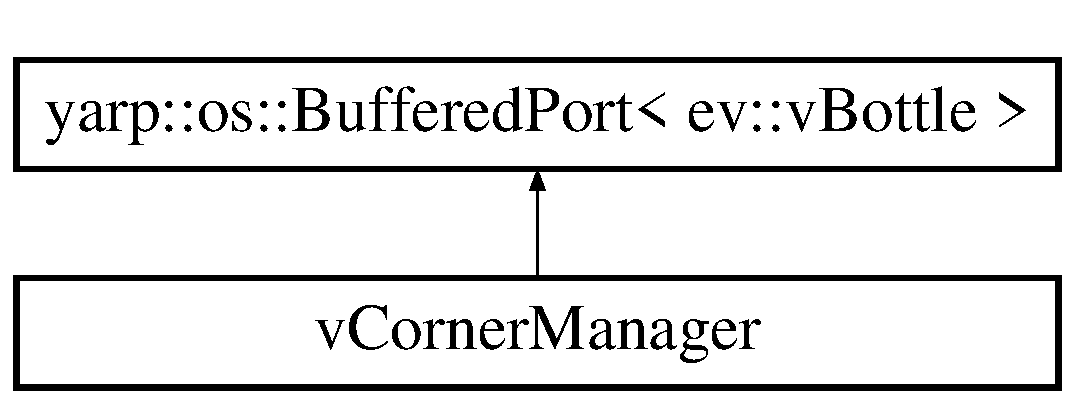
\includegraphics[height=2.000000cm]{classvCornerManager}
\end{center}
\end{figure}
\subsection*{Public Member Functions}
\begin{DoxyCompactItemize}
\item 
{\bfseries v\+Corner\+Manager} (int height, int width, int filter\+Size, int window\+Rad, double sigma, int n\+Events, double thresh)\hypertarget{classvCornerManager_a08e80ac3aafada6b2719cee91649cfa6}{}\label{classvCornerManager_a08e80ac3aafada6b2719cee91649cfa6}

\item 
bool {\bfseries open} (const std\+::string module\+Name, bool strictness=false)\hypertarget{classvCornerManager_ae87a3b35a1047404536af869dd837621}{}\label{classvCornerManager_ae87a3b35a1047404536af869dd837621}

\item 
void {\bfseries close} ()\hypertarget{classvCornerManager_acf1440f33d67878234673e9d4d65a5bf}{}\label{classvCornerManager_acf1440f33d67878234673e9d4d65a5bf}

\item 
void {\bfseries interrupt} ()\hypertarget{classvCornerManager_a360ad86c3e051d7f452bdb4c8d82b28d}{}\label{classvCornerManager_a360ad86c3e051d7f452bdb4c8d82b28d}

\item 
void {\bfseries on\+Read} (\hyperlink{classev_1_1vBottle}{ev\+::v\+Bottle} \&bot)\hypertarget{classvCornerManager_aa67c8b6ded0b19419b294896ddee1803}{}\label{classvCornerManager_aa67c8b6ded0b19419b294896ddee1803}

\end{DoxyCompactItemize}


The documentation for this class was generated from the following files\+:\begin{DoxyCompactItemize}
\item 
/home/aglover/workspace/projects/event-\/driven/src/processing/v\+Corner/include/v\+Corner.\+h\item 
/home/aglover/workspace/projects/event-\/driven/src/processing/v\+Corner/src/v\+Corner.\+cpp\end{DoxyCompactItemize}

\hypertarget{classvCornerModule}{}\section{v\+Corner\+Module Class Reference}
\label{classvCornerModule}\index{v\+Corner\+Module@{v\+Corner\+Module}}
Inheritance diagram for v\+Corner\+Module\+:\begin{figure}[H]
\begin{center}
\leavevmode
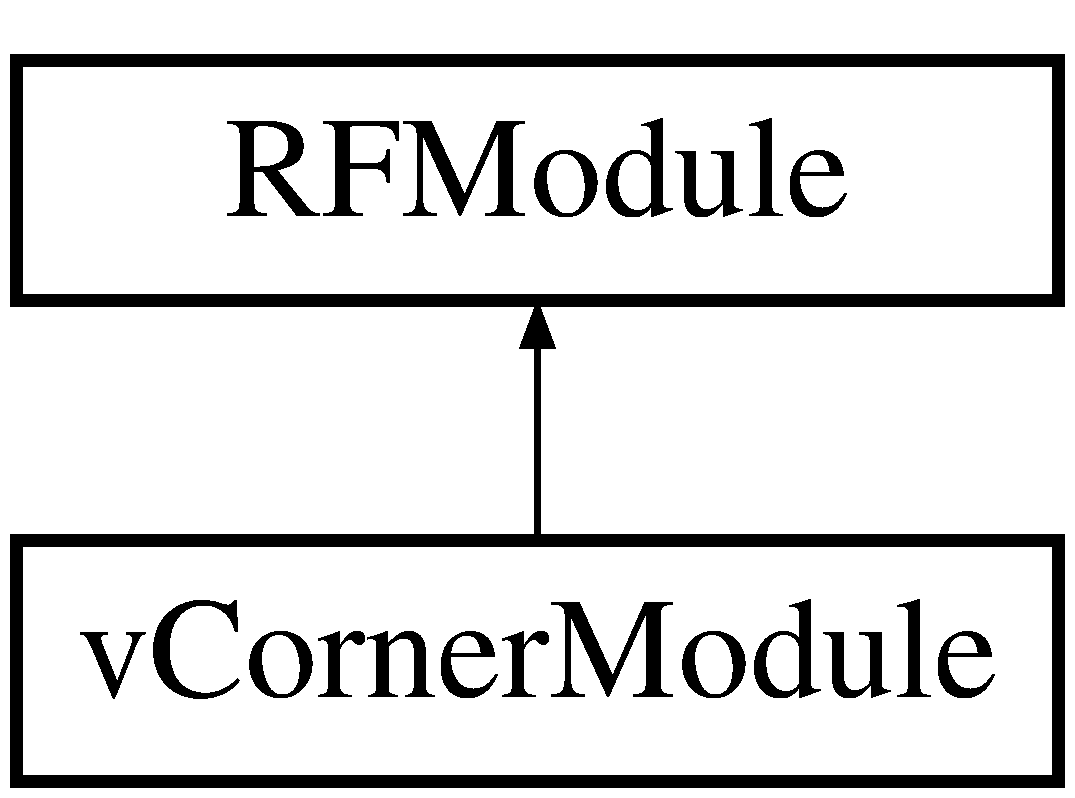
\includegraphics[height=2.000000cm]{classvCornerModule}
\end{center}
\end{figure}
\subsection*{Public Member Functions}
\begin{DoxyCompactItemize}
\item 
virtual bool {\bfseries configure} (yarp\+::os\+::\+Resource\+Finder \&rf)\hypertarget{classvCornerModule_a9496d5d39d6b65dc048ce147ed2856d8}{}\label{classvCornerModule_a9496d5d39d6b65dc048ce147ed2856d8}

\item 
virtual bool {\bfseries interrupt\+Module} ()\hypertarget{classvCornerModule_a8354934bd0d851418e99d93c567f5020}{}\label{classvCornerModule_a8354934bd0d851418e99d93c567f5020}

\item 
virtual bool {\bfseries close} ()\hypertarget{classvCornerModule_aa66707b60e2f920a5faff5c13798b785}{}\label{classvCornerModule_aa66707b60e2f920a5faff5c13798b785}

\item 
virtual double {\bfseries get\+Period} ()\hypertarget{classvCornerModule_afc071a27e74fe3ab6d23a78b25844df4}{}\label{classvCornerModule_afc071a27e74fe3ab6d23a78b25844df4}

\item 
virtual bool {\bfseries update\+Module} ()\hypertarget{classvCornerModule_af25a4ba8a2b8346f0a3a69b6e80998c8}{}\label{classvCornerModule_af25a4ba8a2b8346f0a3a69b6e80998c8}

\end{DoxyCompactItemize}


The documentation for this class was generated from the following files\+:\begin{DoxyCompactItemize}
\item 
/home/aglover/workspace/projects/event-\/driven/src/processing/v\+Corner/include/v\+Corner.\+h\item 
/home/aglover/workspace/projects/event-\/driven/src/processing/v\+Corner/src/v\+Corner.\+cpp\end{DoxyCompactItemize}

\hypertarget{classvDevCtrl}{}\section{v\+Dev\+Ctrl Class Reference}
\label{classvDevCtrl}\index{v\+Dev\+Ctrl@{v\+Dev\+Ctrl}}
\subsection*{Public Member Functions}
\begin{DoxyCompactItemize}
\item 
{\bfseries v\+Dev\+Ctrl} (std\+::string device\+Name=\char`\"{}\char`\"{}, unsigned char i2c\+Address=0)\hypertarget{classvDevCtrl_a28270bc81b8f37400562730649b9ea20}{}\label{classvDevCtrl_a28270bc81b8f37400562730649b9ea20}

\item 
bool {\bfseries set\+Bias} (std\+::string bias\+Name, unsigned int bias\+Value)\hypertarget{classvDevCtrl_ad7c8b642dc056c3e0475af546ed6e534}{}\label{classvDevCtrl_ad7c8b642dc056c3e0475af546ed6e534}

\item 
bool {\bfseries set\+Bias} (yarp\+::os\+::\+Bottle bias)\hypertarget{classvDevCtrl_ac95a8bc8aedcd40fa1fa8089e568390b}{}\label{classvDevCtrl_ac95a8bc8aedcd40fa1fa8089e568390b}

\item 
unsigned int {\bfseries get\+Bias} (std\+::string bias\+Name)\hypertarget{classvDevCtrl_a37baee231dd38b573c674fca0ac0024e}{}\label{classvDevCtrl_a37baee231dd38b573c674fca0ac0024e}

\item 
void {\bfseries use\+Current\+Bias} (bool flag=true)\hypertarget{classvDevCtrl_a051225ff9d84a5699595827e64dc0148}{}\label{classvDevCtrl_a051225ff9d84a5699595827e64dc0148}

\item 
bool {\bfseries connect} (void)\hypertarget{classvDevCtrl_af6ccda24918a78cd5eb800c3f11c07c4}{}\label{classvDevCtrl_af6ccda24918a78cd5eb800c3f11c07c4}

\item 
bool {\bfseries configure} (bool verbose=false)\hypertarget{classvDevCtrl_a432d0c5cb40afbce3e14a685cfdd11c0}{}\label{classvDevCtrl_a432d0c5cb40afbce3e14a685cfdd11c0}

\item 
void {\bfseries disconnect} (bool andturnoff=true)\hypertarget{classvDevCtrl_a274051caa72b84acac607ebb3d7ec2e2}{}\label{classvDevCtrl_a274051caa72b84acac607ebb3d7ec2e2}

\item 
bool {\bfseries activate} (bool active=true)\hypertarget{classvDevCtrl_a737b66cec44fc2bd0ebb29dccf15838b}{}\label{classvDevCtrl_a737b66cec44fc2bd0ebb29dccf15838b}

\item 
bool {\bfseries suspend} (void)\hypertarget{classvDevCtrl_a9cc8b11acf775f7c7afaf736ffe69c52}{}\label{classvDevCtrl_a9cc8b11acf775f7c7afaf736ffe69c52}

\item 
bool {\bfseries configure\+Biases} ()\hypertarget{classvDevCtrl_a33fb7c392cfdaad5c35b7683eacc61e2}{}\label{classvDevCtrl_a33fb7c392cfdaad5c35b7683eacc61e2}

\item 
void {\bfseries print\+Configuration} (void)\hypertarget{classvDevCtrl_a4fc72bb26da523c7c731b9465e19a5cd}{}\label{classvDevCtrl_a4fc72bb26da523c7c731b9465e19a5cd}

\end{DoxyCompactItemize}


The documentation for this class was generated from the following files\+:\begin{DoxyCompactItemize}
\item 
/home/aglover/workspace/projects/event-\/driven/src/hardwareio/zynq\+Grabber/include/device\+Controller.\+h\item 
/home/aglover/workspace/projects/event-\/driven/src/hardwareio/zynq\+Grabber/src/device\+Controller.\+cpp\end{DoxyCompactItemize}

\hypertarget{classvDevReadBuffer}{}\section{v\+Dev\+Read\+Buffer Class Reference}
\label{classvDevReadBuffer}\index{v\+Dev\+Read\+Buffer@{v\+Dev\+Read\+Buffer}}
Inheritance diagram for v\+Dev\+Read\+Buffer\+:\begin{figure}[H]
\begin{center}
\leavevmode
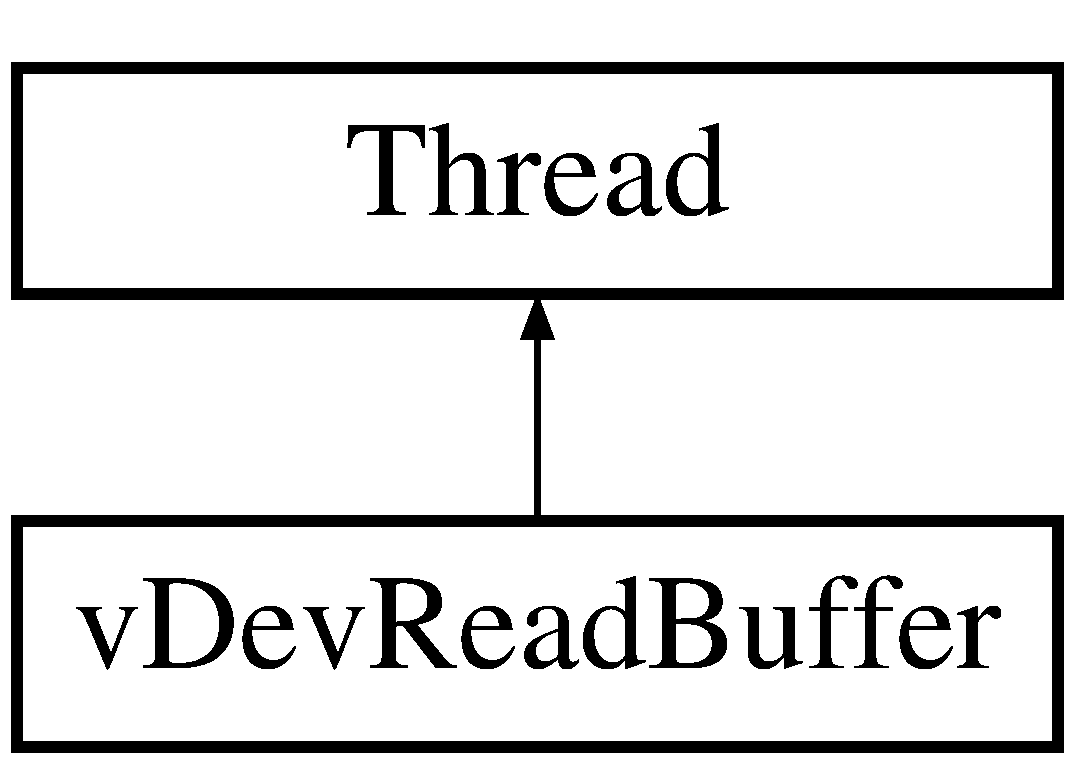
\includegraphics[height=2.000000cm]{classvDevReadBuffer}
\end{center}
\end{figure}
\subsection*{Public Member Functions}
\begin{DoxyCompactItemize}
\item 
bool {\bfseries initialise} (std\+::string devicename, unsigned int buffer\+Size=0, unsigned int read\+Size=0)\hypertarget{classvDevReadBuffer_aed2023a30193768d35ffc3684c826142}{}\label{classvDevReadBuffer_aed2023a30193768d35ffc3684c826142}

\item 
virtual void {\bfseries run} ()\hypertarget{classvDevReadBuffer_a8d3e3995a073efe42d6a8693b66cf87e}{}\label{classvDevReadBuffer_a8d3e3995a073efe42d6a8693b66cf87e}

\item 
virtual void {\bfseries thread\+Release} ()\hypertarget{classvDevReadBuffer_a763f76c090da36846824bbe5a3365278}{}\label{classvDevReadBuffer_a763f76c090da36846824bbe5a3365278}

\item 
std\+::vector$<$ unsigned char $>$ \& {\bfseries get\+Buffer} (unsigned int \&n\+Bytes\+Read, unsigned int \&n\+Bytes\+Lost)\hypertarget{classvDevReadBuffer_a8fd5cc78799d0b9ddcacd958a84c316e}{}\label{classvDevReadBuffer_a8fd5cc78799d0b9ddcacd958a84c316e}

\end{DoxyCompactItemize}


The documentation for this class was generated from the following files\+:\begin{DoxyCompactItemize}
\item 
/home/aglover/workspace/projects/event-\/driven/src/hardwareio/zynq\+Grabber/include/yarp\+Interface.\+h\item 
/home/aglover/workspace/projects/event-\/driven/src/hardwareio/zynq\+Grabber/src/yarp\+Interface.\+cpp\end{DoxyCompactItemize}

\hypertarget{classvDraw}{}\section{v\+Draw Class Reference}
\label{classvDraw}\index{v\+Draw@{v\+Draw}}


The \hyperlink{classvDraw}{v\+Draw} class is the base class from which all v\+Drawers should inherit. It contains the draw and get\+Tag functions which must be overloaded, and the sensor size for reference.  




{\ttfamily \#include $<$v\+Draw.\+h$>$}

Inheritance diagram for v\+Draw\+:\begin{figure}[H]
\begin{center}
\leavevmode
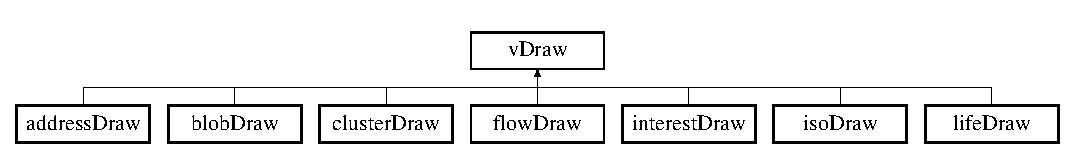
\includegraphics[height=1.684211cm]{classvDraw}
\end{center}
\end{figure}
\subsection*{Public Member Functions}
\begin{DoxyCompactItemize}
\item 
void \hyperlink{classvDraw_a94008d089d3fcc8782b2e175bd0cca59}{set\+Limits} (int Xlimit, int Ylimit)
\begin{DoxyCompactList}\small\item\em set\+Limits sets the maximum possible values of the position of events that could be drawn (mostly governed by the sensor size). \end{DoxyCompactList}\item 
void {\bfseries set\+Window} (int twindow)\hypertarget{classvDraw_a81cc01f4bd16c04124198e72e7bd6d50}{}\label{classvDraw_a81cc01f4bd16c04124198e72e7bd6d50}

\item 
void {\bfseries set\+Flip} (bool flip)\hypertarget{classvDraw_af3f4e8539db44898bb60f8e867f0a3dc}{}\label{classvDraw_af3f4e8539db44898bb60f8e867f0a3dc}

\item 
virtual void {\bfseries initialise} ()\hypertarget{classvDraw_aaea7bac3b19b9004bd60c16d841cfd14}{}\label{classvDraw_aaea7bac3b19b9004bd60c16d841cfd14}

\item 
virtual void \hyperlink{classvDraw_a35cf7b42fe542fd51c1014de19fb114c}{draw} (cv\+::\+Mat \&canvas, const ev\+::v\+Queue \&e\+Set, int v\+Time)=0
\begin{DoxyCompactList}\small\item\em draw takes an image and overlays the new visualisation textures \end{DoxyCompactList}\item 
virtual std\+::string \hyperlink{classvDraw_abb4aa2bb3bb8daca40bdb12cd55d3fd3}{get\+Draw\+Type} ()=0
\begin{DoxyCompactList}\small\item\em get\+Tag returns the unique code for this drawing method. The arguments given on the command line must match this code exactly \end{DoxyCompactList}\item 
virtual std\+::string {\bfseries get\+Event\+Type} ()=0\hypertarget{classvDraw_a9c801e074f399b0e0d9b18cdfd798031}{}\label{classvDraw_a9c801e074f399b0e0d9b18cdfd798031}

\end{DoxyCompactItemize}
\subsection*{Protected Member Functions}
\begin{DoxyCompactItemize}
\item 
int {\bfseries check\+Stagnancy} (const ev\+::v\+Queue \&e\+Set)\hypertarget{classvDraw_a844a978806965028d04bec676755bdd2}{}\label{classvDraw_a844a978806965028d04bec676755bdd2}

\end{DoxyCompactItemize}
\subsection*{Protected Attributes}
\begin{DoxyCompactItemize}
\item 
int {\bfseries Xlimit}\hypertarget{classvDraw_ae8b3fe947b98e624f5a3ec53e8f015b0}{}\label{classvDraw_ae8b3fe947b98e624f5a3ec53e8f015b0}

\item 
int {\bfseries Ylimit}\hypertarget{classvDraw_a5d0ce9dba294b4ce2f286fc940422e04}{}\label{classvDraw_a5d0ce9dba294b4ce2f286fc940422e04}

\item 
int {\bfseries stagnant\+Count}\hypertarget{classvDraw_acabdabb4ad106e6371c7f3b33a19da0e}{}\label{classvDraw_acabdabb4ad106e6371c7f3b33a19da0e}

\item 
int {\bfseries p\+TS}\hypertarget{classvDraw_abb5002dcf2203b5faf2eb2e05351deac}{}\label{classvDraw_abb5002dcf2203b5faf2eb2e05351deac}

\item 
int {\bfseries clear\+Threshold}\hypertarget{classvDraw_af06653835671aa513fffd31d26d99437}{}\label{classvDraw_af06653835671aa513fffd31d26d99437}

\item 
int {\bfseries twindow}\hypertarget{classvDraw_aae409af8476c3f61eb3157887dbde4ad}{}\label{classvDraw_aae409af8476c3f61eb3157887dbde4ad}

\item 
bool {\bfseries flip}\hypertarget{classvDraw_ac2fe76151dac6e58030f4954456b9246}{}\label{classvDraw_ac2fe76151dac6e58030f4954456b9246}

\end{DoxyCompactItemize}


\subsection{Detailed Description}
The \hyperlink{classvDraw}{v\+Draw} class is the base class from which all v\+Drawers should inherit. It contains the draw and get\+Tag functions which must be overloaded, and the sensor size for reference. 

\subsection{Member Function Documentation}
\index{v\+Draw@{v\+Draw}!draw@{draw}}
\index{draw@{draw}!v\+Draw@{v\+Draw}}
\subsubsection[{\texorpdfstring{draw(cv\+::\+Mat \&canvas, const ev\+::v\+Queue \&e\+Set, int v\+Time)=0}{draw(cv::Mat &canvas, const ev::vQueue &eSet, int vTime)=0}}]{\setlength{\rightskip}{0pt plus 5cm}virtual void v\+Draw\+::draw (
\begin{DoxyParamCaption}
\item[{cv\+::\+Mat \&}]{canvas, }
\item[{const ev\+::v\+Queue \&}]{e\+Set, }
\item[{int}]{v\+Time}
\end{DoxyParamCaption}
)\hspace{0.3cm}{\ttfamily [pure virtual]}}\hypertarget{classvDraw_a35cf7b42fe542fd51c1014de19fb114c}{}\label{classvDraw_a35cf7b42fe542fd51c1014de19fb114c}


draw takes an image and overlays the new visualisation textures 


\begin{DoxyParams}{Parameters}
{\em canvas} & is the image which may or may not yet exist \\
\hline
{\em e\+Set} & is the set of events which could possibly be drawn \\
\hline
\end{DoxyParams}


Implemented in \hyperlink{classisoDraw_a20877ef82deb90f2bdea5a3225fc447d}{iso\+Draw}, \hyperlink{classinterestDraw_a0e181779fcbc9303d2f6c77e5151eca8}{interest\+Draw}, \hyperlink{classblobDraw_ae29fcd93142586e3f3ab070f795f26fe}{blob\+Draw}, \hyperlink{classclusterDraw_a4e76b182dc58c06d701e7d44a66de79c}{cluster\+Draw}, \hyperlink{classlifeDraw_af24592ae0bc8be55c7871e17adf6d77b}{life\+Draw}, \hyperlink{classflowDraw_a77d2abe2722b41f045bbea415ac0c858}{flow\+Draw}, and \hyperlink{classaddressDraw_a2eb36efe557d39dfcc49bd5250ec3d6b}{address\+Draw}.

\index{v\+Draw@{v\+Draw}!get\+Draw\+Type@{get\+Draw\+Type}}
\index{get\+Draw\+Type@{get\+Draw\+Type}!v\+Draw@{v\+Draw}}
\subsubsection[{\texorpdfstring{get\+Draw\+Type()=0}{getDrawType()=0}}]{\setlength{\rightskip}{0pt plus 5cm}virtual std\+::string v\+Draw\+::get\+Draw\+Type (
\begin{DoxyParamCaption}
{}
\end{DoxyParamCaption}
)\hspace{0.3cm}{\ttfamily [pure virtual]}}\hypertarget{classvDraw_abb4aa2bb3bb8daca40bdb12cd55d3fd3}{}\label{classvDraw_abb4aa2bb3bb8daca40bdb12cd55d3fd3}


get\+Tag returns the unique code for this drawing method. The arguments given on the command line must match this code exactly 

\begin{DoxyReturn}{Returns}
the tag code 
\end{DoxyReturn}


Implemented in \hyperlink{classisoDraw_a8ff12e0ab9d2b65a16afc175c7cc59c1}{iso\+Draw}, \hyperlink{classinterestDraw_a8121cc47bf53a6571e6afcb1afe68d86}{interest\+Draw}, \hyperlink{classblobDraw_a72b6e196fcd44371a4cdfa734d19dc93}{blob\+Draw}, \hyperlink{classclusterDraw_a1195b2532670913822405dbd8193e0d4}{cluster\+Draw}, \hyperlink{classlifeDraw_a347b92eed9cd308902eecd3346eef5d4}{life\+Draw}, \hyperlink{classflowDraw_a9b2f0523a05825d3d375b43126f6840e}{flow\+Draw}, and \hyperlink{classaddressDraw_a1b1ef76932c71300e87353cc266eb322}{address\+Draw}.

\index{v\+Draw@{v\+Draw}!set\+Limits@{set\+Limits}}
\index{set\+Limits@{set\+Limits}!v\+Draw@{v\+Draw}}
\subsubsection[{\texorpdfstring{set\+Limits(int Xlimit, int Ylimit)}{setLimits(int Xlimit, int Ylimit)}}]{\setlength{\rightskip}{0pt plus 5cm}void v\+Draw\+::set\+Limits (
\begin{DoxyParamCaption}
\item[{int}]{Xlimit, }
\item[{int}]{Ylimit}
\end{DoxyParamCaption}
)\hspace{0.3cm}{\ttfamily [inline]}}\hypertarget{classvDraw_a94008d089d3fcc8782b2e175bd0cca59}{}\label{classvDraw_a94008d089d3fcc8782b2e175bd0cca59}


set\+Limits sets the maximum possible values of the position of events that could be drawn (mostly governed by the sensor size). 


\begin{DoxyParams}{Parameters}
{\em Xlimit} & is the maximum x value (width) \\
\hline
{\em Ylimit} & is the maximium y value (height) \\
\hline
\end{DoxyParams}


The documentation for this class was generated from the following file\+:\begin{DoxyCompactItemize}
\item 
/home/aglover/workspace/projects/event-\/driven/src/processing/v\+Framer/include/v\+Draw.\+h\end{DoxyCompactItemize}

\hypertarget{classev_1_1vEdge}{}\section{ev\+:\+:v\+Edge Class Reference}
\label{classev_1_1vEdge}\index{ev\+::v\+Edge@{ev\+::v\+Edge}}


a spatio-\/temporal surface storing events along edges as given by plane fitting  




{\ttfamily \#include $<$v\+Window\+\_\+adv.\+h$>$}

Inheritance diagram for ev\+:\+:v\+Edge\+:\begin{figure}[H]
\begin{center}
\leavevmode
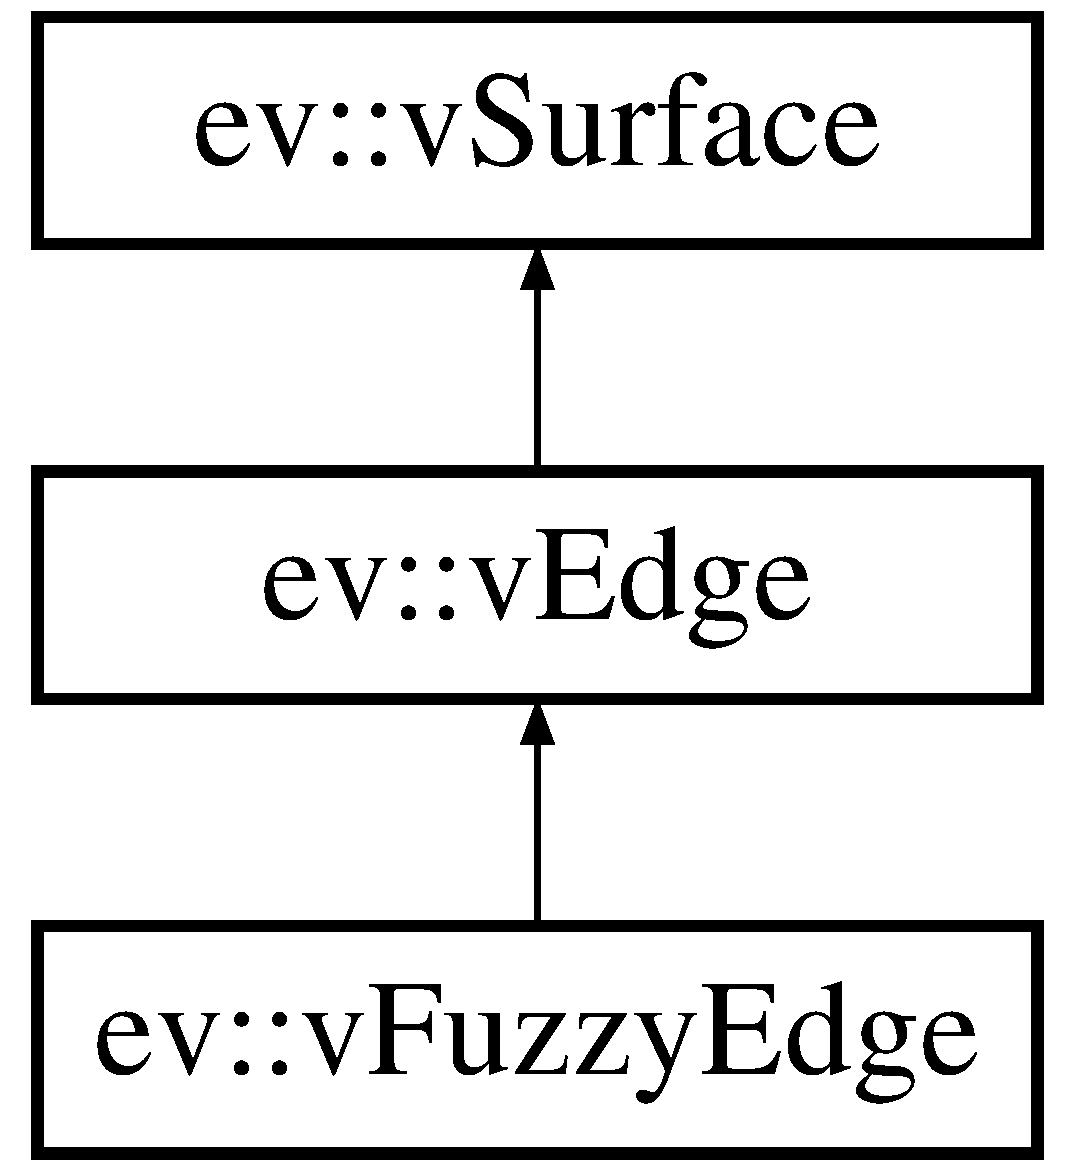
\includegraphics[height=3.000000cm]{classev_1_1vEdge}
\end{center}
\end{figure}
\subsection*{Public Member Functions}
\begin{DoxyCompactItemize}
\item 
{\bfseries v\+Edge} (int width=128, int height=128)\hypertarget{classev_1_1vEdge_a3bbccb1784adbb0543a22e6e1a805be5}{}\label{classev_1_1vEdge_a3bbccb1784adbb0543a22e6e1a805be5}

\item 
v\+Queue {\bfseries add\+Event\+To\+Edge} (event$<$ \hyperlink{classev_1_1AddressEvent}{Address\+Event} $>$ v)\hypertarget{classev_1_1vEdge_a04bc02981fe09b9cc0615a471a4d1594}{}\label{classev_1_1vEdge_a04bc02981fe09b9cc0615a471a4d1594}

\item 
void {\bfseries set\+Thickness} (int pixels)\hypertarget{classev_1_1vEdge_a8add033e36c36c4145d932d8e210750a}{}\label{classev_1_1vEdge_a8add033e36c36c4145d932d8e210750a}

\item 
void {\bfseries track} (bool track\+Count=true)\hypertarget{classev_1_1vEdge_a7e0dd1c7f362d79a0cef3298caa74f8a}{}\label{classev_1_1vEdge_a7e0dd1c7f362d79a0cef3298caa74f8a}

\item 
virtual const v\+Queue {\bfseries get\+Surf} (int xl, int xh, int yl, int yh)\hypertarget{classev_1_1vEdge_a569d6c449ae172b608c0049e9e391e50}{}\label{classev_1_1vEdge_a569d6c449ae172b608c0049e9e391e50}

\end{DoxyCompactItemize}
\subsection*{Additional Inherited Members}


\subsection{Detailed Description}
a spatio-\/temporal surface storing events along edges as given by plane fitting 

The documentation for this class was generated from the following files\+:\begin{DoxyCompactItemize}
\item 
/home/aglover/workspace/projects/event-\/driven/libraries/include/i\+Cub/eventdriven/v\+Window\+\_\+adv.\+h\item 
/home/aglover/workspace/projects/event-\/driven/libraries/src/v\+Window\+\_\+adv.\+cpp\end{DoxyCompactItemize}

\hypertarget{classev_1_1vEvent}{}\section{ev\+:\+:v\+Event Class Reference}
\label{classev_1_1vEvent}\index{ev\+::v\+Event@{ev\+::v\+Event}}


base event class which defines the time the event occurs  




{\ttfamily \#include $<$v\+Codec.\+h$>$}

Inheritance diagram for ev\+:\+:v\+Event\+:\begin{figure}[H]
\begin{center}
\leavevmode
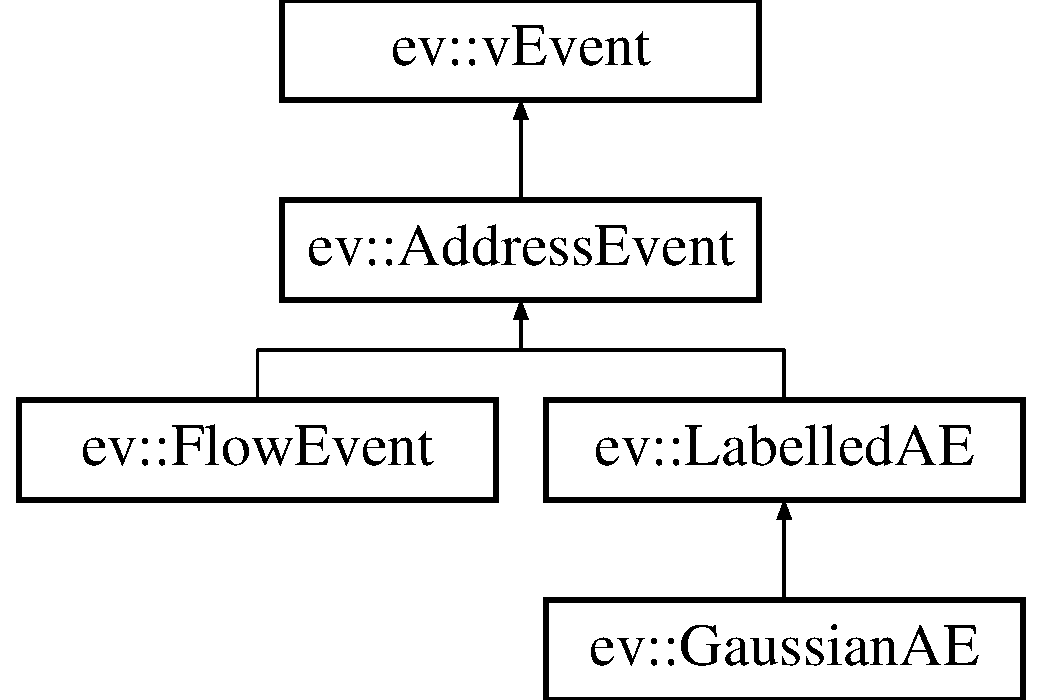
\includegraphics[height=4.000000cm]{classev_1_1vEvent}
\end{center}
\end{figure}
\subsection*{Public Member Functions}
\begin{DoxyCompactItemize}
\item 
virtual event {\bfseries clone} ()\hypertarget{classev_1_1vEvent_a44f88f43a5c6b5aa6d93001a11f9309b}{}\label{classev_1_1vEvent_a44f88f43a5c6b5aa6d93001a11f9309b}

\item 
virtual void {\bfseries encode} (yarp\+::os\+::\+Bottle \&b) const \hypertarget{classev_1_1vEvent_a66d9e4d833031c146cc0ac3af332b1cc}{}\label{classev_1_1vEvent_a66d9e4d833031c146cc0ac3af332b1cc}

\item 
virtual bool {\bfseries decode} (const yarp\+::os\+::\+Bottle \&packet, int \&pos)\hypertarget{classev_1_1vEvent_a75132601bf3f958212fd3793b7e53139}{}\label{classev_1_1vEvent_a75132601bf3f958212fd3793b7e53139}

\item 
virtual yarp\+::os\+::\+Property {\bfseries get\+Content} () const \hypertarget{classev_1_1vEvent_adabb906a71f96c89d6d539c899044622}{}\label{classev_1_1vEvent_adabb906a71f96c89d6d539c899044622}

\item 
virtual std\+::string {\bfseries get\+Type} () const \hypertarget{classev_1_1vEvent_a90411228dd74d994854b501b7cae7ff1}{}\label{classev_1_1vEvent_a90411228dd74d994854b501b7cae7ff1}

\item 
virtual int {\bfseries get\+Channel} () const \hypertarget{classev_1_1vEvent_a8ddb67938981d00a7275417e511ad3a5}{}\label{classev_1_1vEvent_a8ddb67938981d00a7275417e511ad3a5}

\item 
virtual void {\bfseries set\+Channel} ()\hypertarget{classev_1_1vEvent_a2cf5bf1d01ad2757a82b6e07d7e2a5da}{}\label{classev_1_1vEvent_a2cf5bf1d01ad2757a82b6e07d7e2a5da}

\end{DoxyCompactItemize}
\subsection*{Public Attributes}
\begin{DoxyCompactItemize}
\item 
unsigned int {\bfseries stamp}\+:31\hypertarget{classev_1_1vEvent_ad4e003653fa59b37682addefce835490}{}\label{classev_1_1vEvent_ad4e003653fa59b37682addefce835490}

\end{DoxyCompactItemize}
\subsection*{Static Public Attributes}
\begin{DoxyCompactItemize}
\item 
static const std\+::string {\bfseries tag} = \char`\"{}TS\char`\"{}\hypertarget{classev_1_1vEvent_a54bcc0830c5993b56f1f47e23df1de8e}{}\label{classev_1_1vEvent_a54bcc0830c5993b56f1f47e23df1de8e}

\end{DoxyCompactItemize}


\subsection{Detailed Description}
base event class which defines the time the event occurs 

The documentation for this class was generated from the following files\+:\begin{DoxyCompactItemize}
\item 
/home/aglover/workspace/projects/event-\/driven/libraries/include/i\+Cub/eventdriven/v\+Codec.\+h\item 
/home/aglover/workspace/projects/event-\/driven/libraries/src/codecs/codec\+\_\+v\+Event.\+cpp\end{DoxyCompactItemize}

\hypertarget{classvFlowManager}{}\section{v\+Flow\+Manager Class Reference}
\label{classvFlowManager}\index{v\+Flow\+Manager@{v\+Flow\+Manager}}
Inheritance diagram for v\+Flow\+Manager\+:\begin{figure}[H]
\begin{center}
\leavevmode
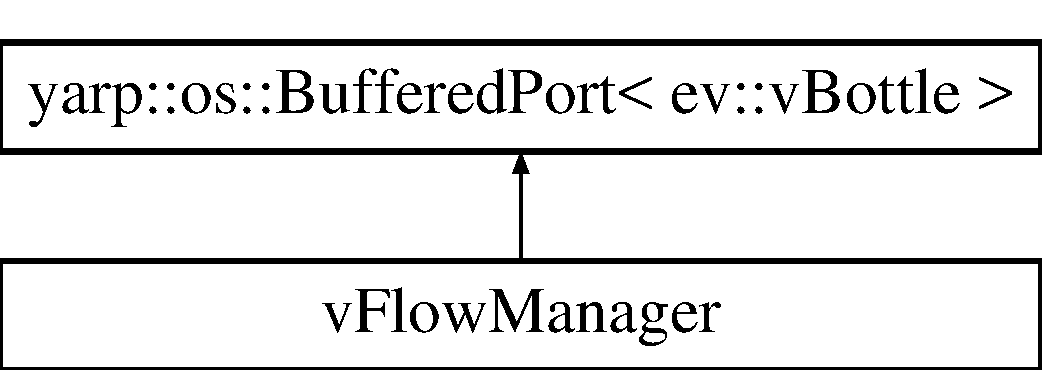
\includegraphics[height=2.000000cm]{classvFlowManager}
\end{center}
\end{figure}
\subsection*{Public Member Functions}
\begin{DoxyCompactItemize}
\item 
{\bfseries v\+Flow\+Manager} (int height, int width, int filter\+Size, int min\+Evts\+On\+Plane)\hypertarget{classvFlowManager_a9d28c98ce6f6c0591a89f5055153e295}{}\label{classvFlowManager_a9d28c98ce6f6c0591a89f5055153e295}

\item 
bool {\bfseries open} (std\+::string module\+Name, bool strictness=false)\hypertarget{classvFlowManager_a2c299db37662565d5b0c59679b790a4b}{}\label{classvFlowManager_a2c299db37662565d5b0c59679b790a4b}

\item 
void {\bfseries close} ()\hypertarget{classvFlowManager_abcf434ef8391ec6741c0754bc4a88ab8}{}\label{classvFlowManager_abcf434ef8391ec6741c0754bc4a88ab8}

\item 
void {\bfseries interrupt} ()\hypertarget{classvFlowManager_a10d85ce69f60a672adba81aff4a046d8}{}\label{classvFlowManager_a10d85ce69f60a672adba81aff4a046d8}

\item 
void {\bfseries on\+Read} (\hyperlink{classev_1_1vBottle}{ev\+::v\+Bottle} \&in\+Bottle)\hypertarget{classvFlowManager_a9749ff591f71a96735692ce1520c9e30}{}\label{classvFlowManager_a9749ff591f71a96735692ce1520c9e30}

\end{DoxyCompactItemize}


The documentation for this class was generated from the following files\+:\begin{DoxyCompactItemize}
\item 
/home/aglover/workspace/projects/event-\/driven/src/processing/v\+Flow/include/v\+Flow.\+h\item 
/home/aglover/workspace/projects/event-\/driven/src/processing/v\+Flow/src/v\+Flow.\+cpp\end{DoxyCompactItemize}

\hypertarget{classvFlowModule}{}\section{v\+Flow\+Module Class Reference}
\label{classvFlowModule}\index{v\+Flow\+Module@{v\+Flow\+Module}}
Inheritance diagram for v\+Flow\+Module\+:\begin{figure}[H]
\begin{center}
\leavevmode
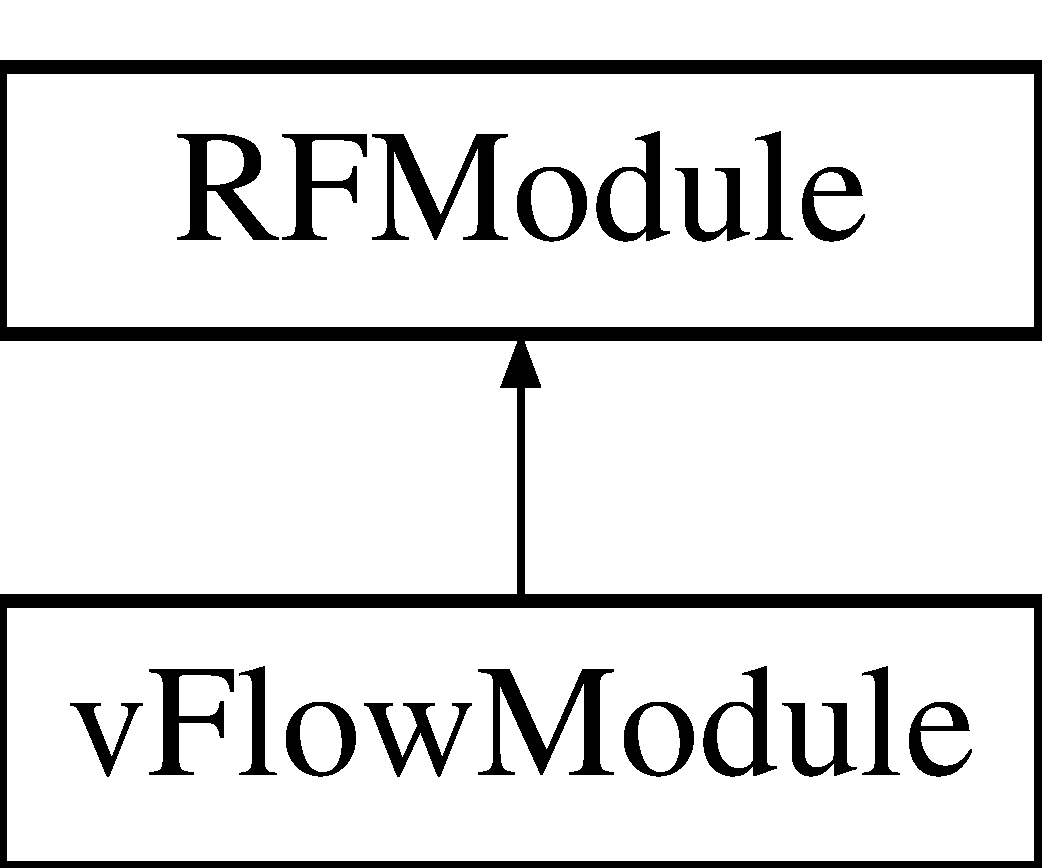
\includegraphics[height=2.000000cm]{classvFlowModule}
\end{center}
\end{figure}
\subsection*{Public Member Functions}
\begin{DoxyCompactItemize}
\item 
virtual bool {\bfseries configure} (yarp\+::os\+::\+Resource\+Finder \&rf)\hypertarget{classvFlowModule_a5cf91bc0de9e311b1946c6ec044fd947}{}\label{classvFlowModule_a5cf91bc0de9e311b1946c6ec044fd947}

\item 
virtual bool {\bfseries interrupt\+Module} ()\hypertarget{classvFlowModule_a49a90a2d595d99bf290423dd930eefe2}{}\label{classvFlowModule_a49a90a2d595d99bf290423dd930eefe2}

\item 
virtual bool {\bfseries close} ()\hypertarget{classvFlowModule_a63a3da2ac7ba9631753ea244d8bc4358}{}\label{classvFlowModule_a63a3da2ac7ba9631753ea244d8bc4358}

\item 
virtual bool {\bfseries update\+Module} ()\hypertarget{classvFlowModule_a880de21f5c85d684f7c0999d0a84e26b}{}\label{classvFlowModule_a880de21f5c85d684f7c0999d0a84e26b}

\item 
virtual double {\bfseries get\+Period} ()\hypertarget{classvFlowModule_a8f6f74c4a7888e162c2dff8a34a84323}{}\label{classvFlowModule_a8f6f74c4a7888e162c2dff8a34a84323}

\end{DoxyCompactItemize}


The documentation for this class was generated from the following files\+:\begin{DoxyCompactItemize}
\item 
/home/aglover/workspace/projects/event-\/driven/src/processing/v\+Flow/include/v\+Flow.\+h\item 
/home/aglover/workspace/projects/event-\/driven/src/processing/v\+Flow/src/v\+Flow.\+cpp\end{DoxyCompactItemize}

\hypertarget{classvFramerModule}{}\section{v\+Framer\+Module Class Reference}
\label{classvFramerModule}\index{v\+Framer\+Module@{v\+Framer\+Module}}


The \hyperlink{classvFramerModule}{v\+Framer\+Module} class runs the event reading and channel splitting, the drawing modules, and the yarp image output buffers. Images are created at a rate equal to the rate of this thread.  




{\ttfamily \#include $<$v\+Framer.\+h$>$}

Inheritance diagram for v\+Framer\+Module\+:\begin{figure}[H]
\begin{center}
\leavevmode
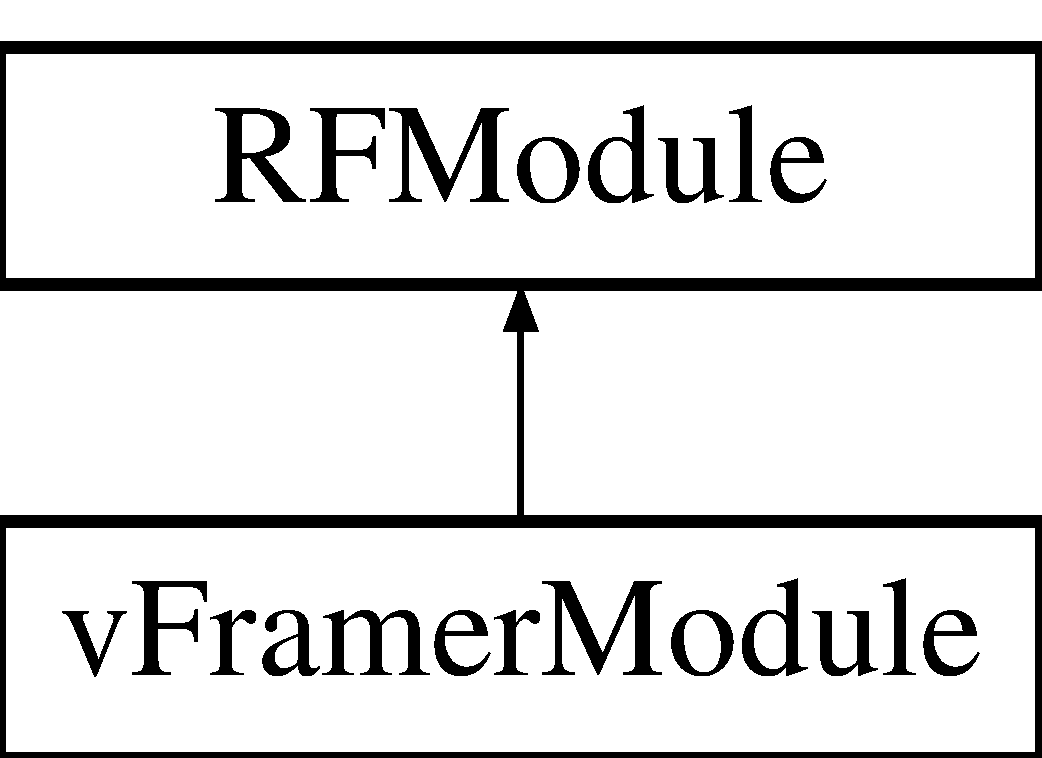
\includegraphics[height=2.000000cm]{classvFramerModule}
\end{center}
\end{figure}
\subsection*{Public Member Functions}
\begin{DoxyCompactItemize}
\item 
virtual bool {\bfseries configure} (yarp\+::os\+::\+Resource\+Finder \&rf)\hypertarget{classvFramerModule_a68f4d912eec9fb85e56c7d1b17cb678b}{}\label{classvFramerModule_a68f4d912eec9fb85e56c7d1b17cb678b}

\item 
virtual bool {\bfseries interrupt\+Module} ()\hypertarget{classvFramerModule_a0e346732e0e922007a27cffbc337c595}{}\label{classvFramerModule_a0e346732e0e922007a27cffbc337c595}

\item 
virtual bool {\bfseries close} ()\hypertarget{classvFramerModule_a132ce95e54786b24864dbd58f660d957}{}\label{classvFramerModule_a132ce95e54786b24864dbd58f660d957}

\item 
virtual bool {\bfseries update\+Module} ()\hypertarget{classvFramerModule_a4169d6f2c241299a513cc87793e05be3}{}\label{classvFramerModule_a4169d6f2c241299a513cc87793e05be3}

\item 
virtual double {\bfseries get\+Period} ()\hypertarget{classvFramerModule_a99439fb2c0b0c06b8dd0e31261ede4ab}{}\label{classvFramerModule_a99439fb2c0b0c06b8dd0e31261ede4ab}

\end{DoxyCompactItemize}


\subsection{Detailed Description}
The \hyperlink{classvFramerModule}{v\+Framer\+Module} class runs the event reading and channel splitting, the drawing modules, and the yarp image output buffers. Images are created at a rate equal to the rate of this thread. 

The documentation for this class was generated from the following files\+:\begin{DoxyCompactItemize}
\item 
/home/aglover/workspace/projects/event-\/driven/src/processing/v\+Framer/include/v\+Framer.\+h\item 
/home/aglover/workspace/projects/event-\/driven/src/processing/v\+Framer/src/v\+Framer.\+cpp\end{DoxyCompactItemize}

\hypertarget{classev_1_1vFuzzyEdge}{}\section{ev\+:\+:v\+Fuzzy\+Edge Class Reference}
\label{classev_1_1vFuzzyEdge}\index{ev\+::v\+Fuzzy\+Edge@{ev\+::v\+Fuzzy\+Edge}}


a \hyperlink{classev_1_1vEdge}{v\+Edge} structure that keeps events given a \char`\"{}fuzzy\char`\"{} scoring system  




{\ttfamily \#include $<$v\+Window\+\_\+adv.\+h$>$}

Inheritance diagram for ev\+:\+:v\+Fuzzy\+Edge\+:\begin{figure}[H]
\begin{center}
\leavevmode
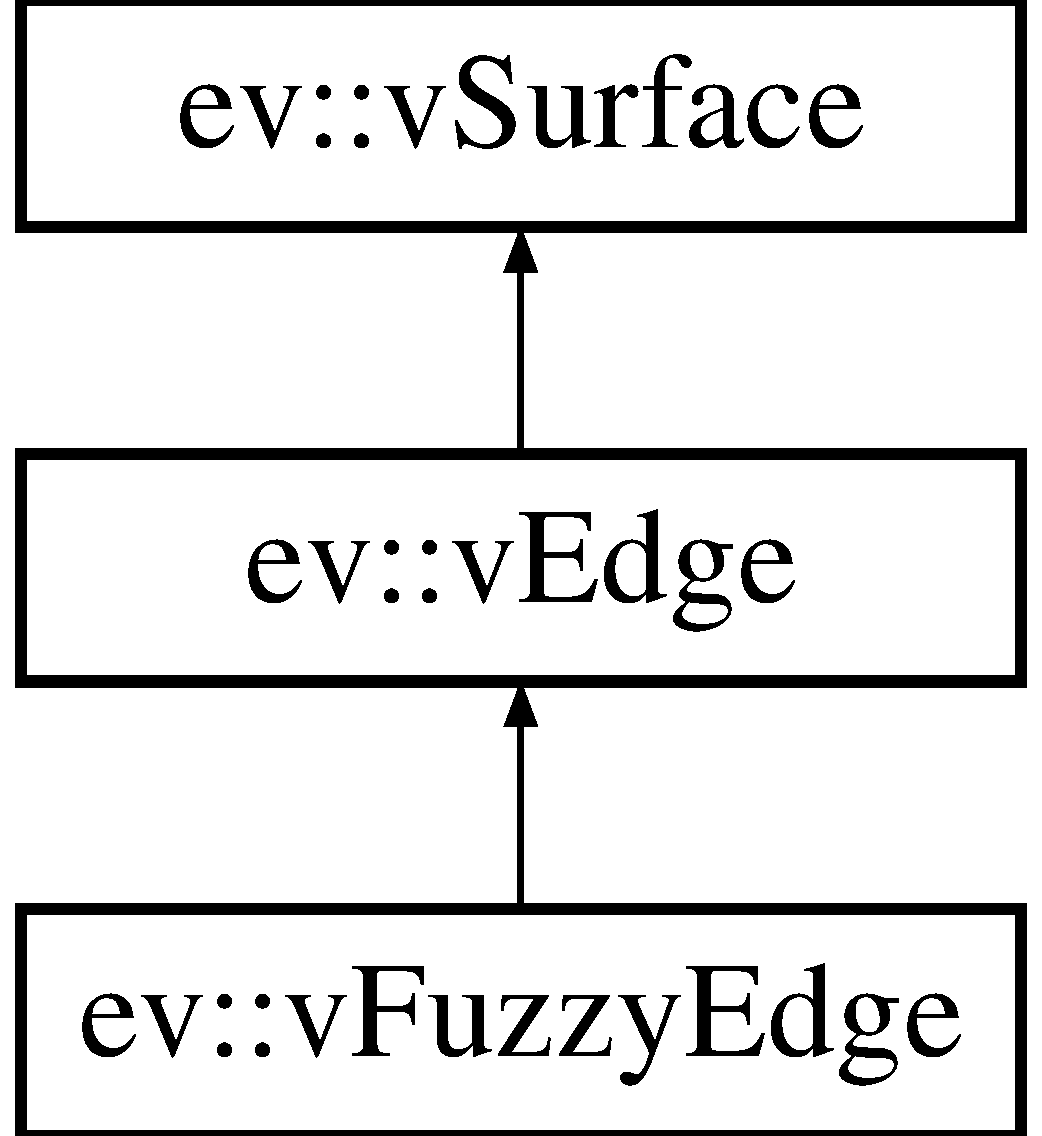
\includegraphics[height=3.000000cm]{classev_1_1vFuzzyEdge}
\end{center}
\end{figure}
\subsection*{Public Member Functions}
\begin{DoxyCompactItemize}
\item 
{\bfseries v\+Fuzzy\+Edge} (int width=128, int height=128, double delta=0.\+4)\hypertarget{classev_1_1vFuzzyEdge_a4fa6e20618a528a591baf2f098cace53}{}\label{classev_1_1vFuzzyEdge_a4fa6e20618a528a591baf2f098cace53}

\item 
v\+Queue {\bfseries add\+Event\+To\+Edge} (event$<$ \hyperlink{classev_1_1AddressEvent}{Address\+Event} $>$ event)\hypertarget{classev_1_1vFuzzyEdge_a61803b783119945df5c130c12d99e9c2}{}\label{classev_1_1vFuzzyEdge_a61803b783119945df5c130c12d99e9c2}

\item 
virtual const v\+Queue {\bfseries get\+S\+U\+RF} (int xl, int xh, int yl, int yh)\hypertarget{classev_1_1vFuzzyEdge_a335aeb48314d3e2068a55ee0a6958643}{}\label{classev_1_1vFuzzyEdge_a335aeb48314d3e2068a55ee0a6958643}

\end{DoxyCompactItemize}
\subsection*{Additional Inherited Members}


\subsection{Detailed Description}
a \hyperlink{classev_1_1vEdge}{v\+Edge} structure that keeps events given a \char`\"{}fuzzy\char`\"{} scoring system 

The documentation for this class was generated from the following files\+:\begin{DoxyCompactItemize}
\item 
/home/aglover/workspace/projects/event-\/driven/libraries/include/i\+Cub/eventdriven/v\+Window\+\_\+adv.\+h\item 
/home/aglover/workspace/projects/event-\/driven/libraries/src/v\+Window\+\_\+adv.\+cpp\end{DoxyCompactItemize}

\hypertarget{classev_1_1vNoiseFilter}{}\section{ev\+:\+:v\+Noise\+Filter Class Reference}
\label{classev_1_1vNoiseFilter}\index{ev\+::v\+Noise\+Filter@{ev\+::v\+Noise\+Filter}}


an efficient event-\/based salt and pepper filter  




{\ttfamily \#include $<$v\+Filters.\+h$>$}

\subsection*{Public Member Functions}
\begin{DoxyCompactItemize}
\item 
void {\bfseries initialise} (double width, double height, int Tsize, unsigned int Ssize)\hypertarget{classev_1_1vNoiseFilter_af7c6cf000f7ed7193d160debac4e6879}{}\label{classev_1_1vNoiseFilter_af7c6cf000f7ed7193d160debac4e6879}

\item 
bool {\bfseries check} (int x, int y, int p, int c, int ts)\hypertarget{classev_1_1vNoiseFilter_a71ed5ded4f59d1c3180b0f5e5a021547}{}\label{classev_1_1vNoiseFilter_a71ed5ded4f59d1c3180b0f5e5a021547}

\end{DoxyCompactItemize}


\subsection{Detailed Description}
an efficient event-\/based salt and pepper filter 

The documentation for this class was generated from the following file\+:\begin{DoxyCompactItemize}
\item 
/home/aglover/workspace/projects/event-\/driven/libraries/include/i\+Cub/eventdriven/v\+Filters.\+h\end{DoxyCompactItemize}

\hypertarget{classvParticle}{}\section{v\+Particle Class Reference}
\label{classvParticle}\index{v\+Particle@{v\+Particle}}
\subsection*{Public Member Functions}
\begin{DoxyCompactItemize}
\item 
\hyperlink{classvParticle}{v\+Particle} \& {\bfseries operator=} (const \hyperlink{classvParticle}{v\+Particle} \&rhs)\hypertarget{classvParticle_a7e2a56a487ab19d6b17ffd8fd26cf83e}{}\label{classvParticle_a7e2a56a487ab19d6b17ffd8fd26cf83e}

\item 
void {\bfseries initialise\+Parameters} (int id, double min\+Likelihood, double outlier\+Param, double inlier\+Param, double variance, int angbuckets)\hypertarget{classvParticle_aefc50d1edaeac94dd1fc58719cf8fb64}{}\label{classvParticle_aefc50d1edaeac94dd1fc58719cf8fb64}

\item 
void {\bfseries attach\+P\+CB} (\hyperlink{classpreComputedBins}{pre\+Computed\+Bins} $\ast$pcb)\hypertarget{classvParticle_a83f71814b1a873e5641e35d8e46439db}{}\label{classvParticle_a83f71814b1a873e5641e35d8e46439db}

\item 
void {\bfseries initialise\+State} (double x, double y, double r, double tw)\hypertarget{classvParticle_a6e4bf2f8057efb01ee6a24da7724a099}{}\label{classvParticle_a6e4bf2f8057efb01ee6a24da7724a099}

\item 
void {\bfseries randomise} (int x, int y, int r, int tw)\hypertarget{classvParticle_a4c7b748b2537bff55c893b4f6bc6ab39}{}\label{classvParticle_a4c7b748b2537bff55c893b4f6bc6ab39}

\item 
void {\bfseries reset\+Stamp} (unsigned long int value)\hypertarget{classvParticle_abefd506d8def5255654736e471db8a6d}{}\label{classvParticle_abefd506d8def5255654736e471db8a6d}

\item 
void {\bfseries reset\+Weight} (double value)\hypertarget{classvParticle_aaa4c200b9a67deb457e55d06672e16cf}{}\label{classvParticle_aaa4c200b9a67deb457e55d06672e16cf}

\item 
void {\bfseries reset\+Radius} (double value)\hypertarget{classvParticle_a20fca983783950a35bcc737ebd705d0b}{}\label{classvParticle_a20fca983783950a35bcc737ebd705d0b}

\item 
void {\bfseries predict} (unsigned long int stamp)\hypertarget{classvParticle_a4f577057ec03af89721ff0abf3daaf5a}{}\label{classvParticle_a4f577057ec03af89721ff0abf3daaf5a}

\item 
void {\bfseries init\+Likelihood} ()\hypertarget{classvParticle_aeb6f48a94882492e7959cab8cc670714}{}\label{classvParticle_aeb6f48a94882492e7959cab8cc670714}

\item 
int {\bfseries incremental\+Likelihood} (int vx, int vy, int dt)\hypertarget{classvParticle_ad99a216eb8cc0ac87385777919a21267}{}\label{classvParticle_ad99a216eb8cc0ac87385777919a21267}

\item 
void {\bfseries conclude\+Likelihood} ()\hypertarget{classvParticle_ae16c098e00f11d2858edef59fc323c53}{}\label{classvParticle_ae16c098e00f11d2858edef59fc323c53}

\item 
void {\bfseries update\+Weight\+Sync} (double normval)\hypertarget{classvParticle_a71ac3f26d797818df2c671cb63ef5a60}{}\label{classvParticle_a71ac3f26d797818df2c671cb63ef5a60}

\item 
int {\bfseries getid} ()\hypertarget{classvParticle_a121f7c012ccbb6153eda5bee38ba310b}{}\label{classvParticle_a121f7c012ccbb6153eda5bee38ba310b}

\item 
double {\bfseries getx} ()\hypertarget{classvParticle_a3d198bc0a1b1a475ab0b044bbff61488}{}\label{classvParticle_a3d198bc0a1b1a475ab0b044bbff61488}

\item 
double {\bfseries gety} ()\hypertarget{classvParticle_a40050ef035199b05e7cfd2601003d68a}{}\label{classvParticle_a40050ef035199b05e7cfd2601003d68a}

\item 
double {\bfseries getr} ()\hypertarget{classvParticle_ac78d2469a78798f791a5dab9f69b732e}{}\label{classvParticle_ac78d2469a78798f791a5dab9f69b732e}

\item 
double {\bfseries getw} ()\hypertarget{classvParticle_ac75939f4ac46ee086991fb629c583ada}{}\label{classvParticle_ac75939f4ac46ee086991fb629c583ada}

\item 
double {\bfseries getl} ()\hypertarget{classvParticle_a9b43157a0b2b278873c78806ccd75f6f}{}\label{classvParticle_a9b43157a0b2b278873c78806ccd75f6f}

\item 
double {\bfseries gettw} ()\hypertarget{classvParticle_a1760cb3cbd3014e6f5cf0a55e5d4dfff}{}\label{classvParticle_a1760cb3cbd3014e6f5cf0a55e5d4dfff}

\end{DoxyCompactItemize}


The documentation for this class was generated from the following files\+:\begin{DoxyCompactItemize}
\item 
/home/aglover/workspace/projects/event-\/driven/src/processing/v\+Particle\+Filter/include/v\+Particle.\+h\item 
/home/aglover/workspace/projects/event-\/driven/src/processing/v\+Particle\+Filter/src/v\+Particle.\+cpp\end{DoxyCompactItemize}

\hypertarget{classvParticleModule}{}\section{v\+Particle\+Module Class Reference}
\label{classvParticleModule}\index{v\+Particle\+Module@{v\+Particle\+Module}}
Inheritance diagram for v\+Particle\+Module\+:\begin{figure}[H]
\begin{center}
\leavevmode
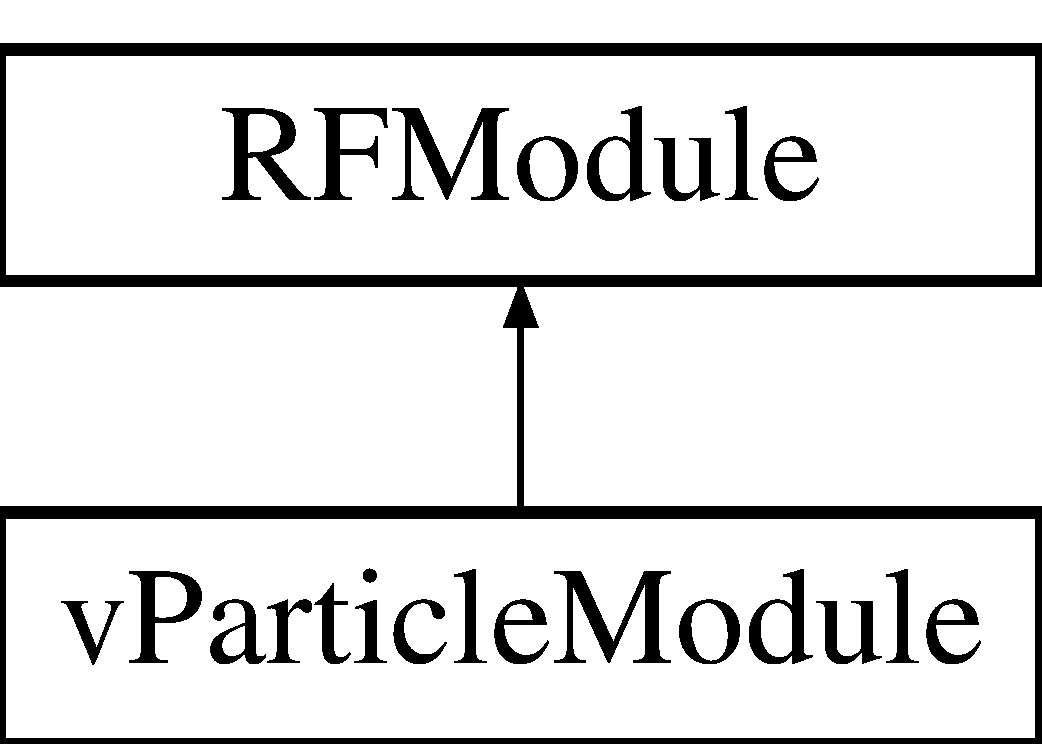
\includegraphics[height=2.000000cm]{classvParticleModule}
\end{center}
\end{figure}
\subsection*{Public Member Functions}
\begin{DoxyCompactItemize}
\item 
virtual bool {\bfseries configure} (yarp\+::os\+::\+Resource\+Finder \&rf)\hypertarget{classvParticleModule_a50220d0e8c348cbb887924def82ec78b}{}\label{classvParticleModule_a50220d0e8c348cbb887924def82ec78b}

\item 
virtual bool {\bfseries interrupt\+Module} ()\hypertarget{classvParticleModule_ae0dbee0680f7006c09a2413d13cbb4fb}{}\label{classvParticleModule_ae0dbee0680f7006c09a2413d13cbb4fb}

\item 
virtual bool {\bfseries close} ()\hypertarget{classvParticleModule_a622f526fc7e2e194b301ff1fa6a362bb}{}\label{classvParticleModule_a622f526fc7e2e194b301ff1fa6a362bb}

\item 
virtual double {\bfseries get\+Period} ()\hypertarget{classvParticleModule_acee72c3ad5f6eddb580fbf57f0cb9d7e}{}\label{classvParticleModule_acee72c3ad5f6eddb580fbf57f0cb9d7e}

\item 
virtual bool {\bfseries update\+Module} ()\hypertarget{classvParticleModule_ae1973b925b09372518b4922b8f033363}{}\label{classvParticleModule_ae1973b925b09372518b4922b8f033363}

\end{DoxyCompactItemize}


The documentation for this class was generated from the following files\+:\begin{DoxyCompactItemize}
\item 
/home/aglover/workspace/projects/event-\/driven/src/processing/v\+Particle\+Filter/include/v\+Particle\+Module.\+h\item 
/home/aglover/workspace/projects/event-\/driven/src/processing/v\+Particle\+Filter/src/v\+Particle\+Module.\+cpp\end{DoxyCompactItemize}

\hypertarget{classvParticleReader}{}\section{v\+Particle\+Reader Class Reference}
\label{classvParticleReader}\index{v\+Particle\+Reader@{v\+Particle\+Reader}}
Inheritance diagram for v\+Particle\+Reader\+:\begin{figure}[H]
\begin{center}
\leavevmode
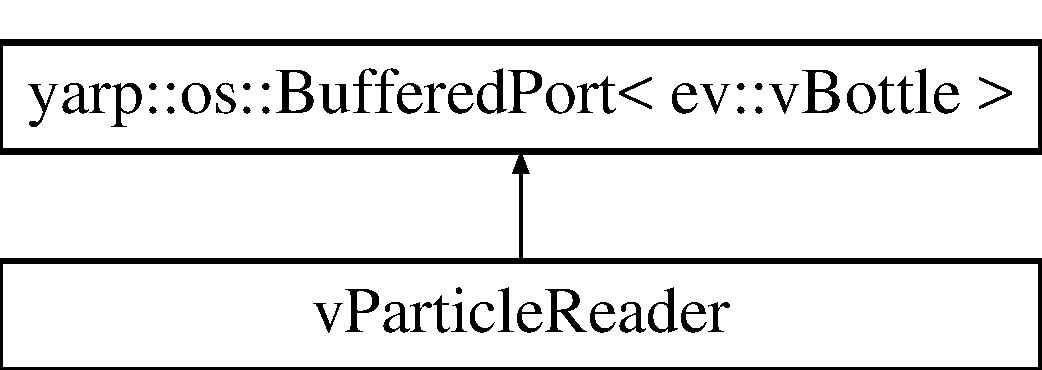
\includegraphics[height=2.000000cm]{classvParticleReader}
\end{center}
\end{figure}
\subsection*{Public Member Functions}
\begin{DoxyCompactItemize}
\item 
void {\bfseries initialise} (unsigned int width, unsigned int height, unsigned int n\+Particles, unsigned int rate, double n\+Rands, bool adaptive, double p\+Variance, int camera, bool use\+R\+OI)\hypertarget{classvParticleReader_a423292f63faa86c5da923d7500166775}{}\label{classvParticleReader_a423292f63faa86c5da923d7500166775}

\item 
void {\bfseries set\+Observation\+Parameters} (double min\+Likelihood, double inlier\+Par, double outlier\+Par)\hypertarget{classvParticleReader_a07ef00d6c0f4f7b4f975e32d9a7cbbb6}{}\label{classvParticleReader_a07ef00d6c0f4f7b4f975e32d9a7cbbb6}

\item 
void {\bfseries set\+Seed} (int x, int y, int r)\hypertarget{classvParticleReader_a0025952cf4957b8eeedfff63e386ded4}{}\label{classvParticleReader_a0025952cf4957b8eeedfff63e386ded4}

\item 
bool {\bfseries open} (const std\+::string \&name, bool strictness=false)\hypertarget{classvParticleReader_a758adac809850f3fc1f01d2502d609bc}{}\label{classvParticleReader_a758adac809850f3fc1f01d2502d609bc}

\item 
void {\bfseries on\+Read} (\hyperlink{classev_1_1vBottle}{ev\+::v\+Bottle} \&in\+Bot)\hypertarget{classvParticleReader_af4bb9d631985a90d797416eca04777bb}{}\label{classvParticleReader_af4bb9d631985a90d797416eca04777bb}

\item 
void {\bfseries close} ()\hypertarget{classvParticleReader_a727d94974d16c502ac2518c5760e0fcc}{}\label{classvParticleReader_a727d94974d16c502ac2518c5760e0fcc}

\item 
void {\bfseries interrupt} ()\hypertarget{classvParticleReader_af7e95400429bb07bc9a438f8a163023e}{}\label{classvParticleReader_af7e95400429bb07bc9a438f8a163023e}

\end{DoxyCompactItemize}


The documentation for this class was generated from the following files\+:\begin{DoxyCompactItemize}
\item 
/home/aglover/workspace/projects/event-\/driven/src/processing/v\+Particle\+Filter/include/v\+Fixed\+Rate.\+h\item 
/home/aglover/workspace/projects/event-\/driven/src/processing/v\+Particle\+Filter/src/v\+Fixed\+Rate.\+cpp\end{DoxyCompactItemize}

\hypertarget{classvPartObsThread}{}\section{v\+Part\+Obs\+Thread Class Reference}
\label{classvPartObsThread}\index{v\+Part\+Obs\+Thread@{v\+Part\+Obs\+Thread}}
Inheritance diagram for v\+Part\+Obs\+Thread\+:\begin{figure}[H]
\begin{center}
\leavevmode
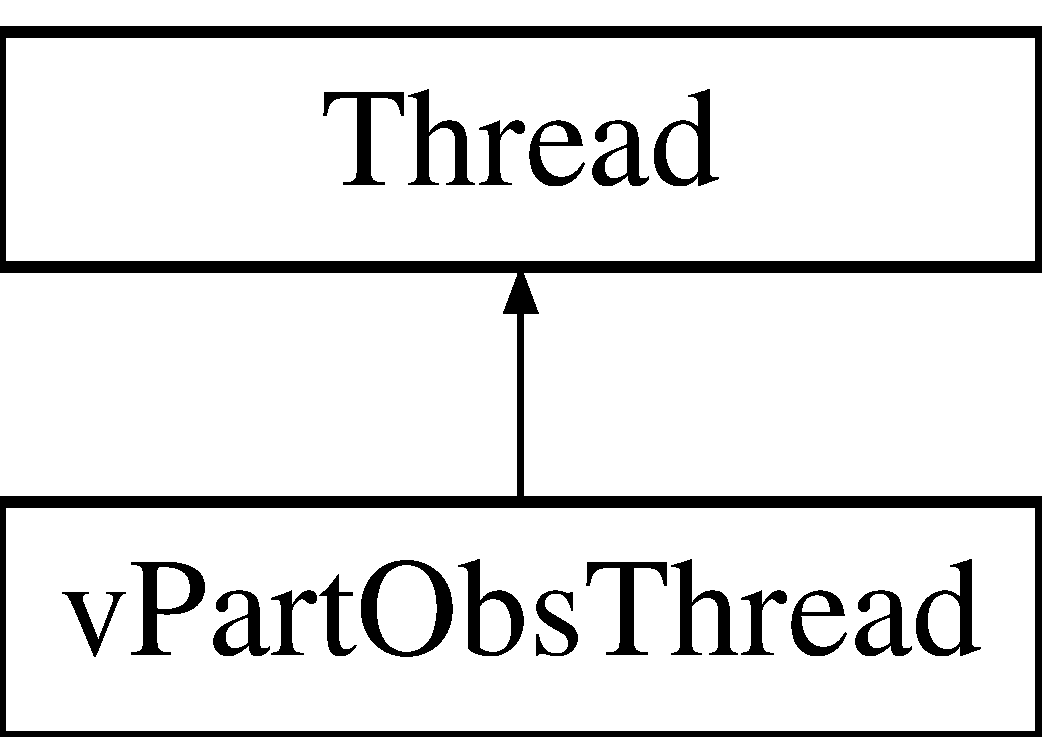
\includegraphics[height=2.000000cm]{classvPartObsThread}
\end{center}
\end{figure}
\subsection*{Public Member Functions}
\begin{DoxyCompactItemize}
\item 
{\bfseries v\+Part\+Obs\+Thread} (int p\+Start, int p\+End)\hypertarget{classvPartObsThread_ad5ee91bcd5ace1cac76ac13843597d3d}{}\label{classvPartObsThread_ad5ee91bcd5ace1cac76ac13843597d3d}

\item 
void {\bfseries set\+Data\+Sources} (std\+::vector$<$ \hyperlink{classvParticle}{v\+Particle} $>$ $\ast$particles, std\+::vector$<$ int $>$ $\ast$deltats, ev\+::v\+Queue $\ast$stw, yarp\+::sig\+::\+Image\+Of$<$ yarp\+::sig\+::\+Pixel\+Bgr $>$ $\ast$debug\+Im)\hypertarget{classvPartObsThread_a2e85818df4f193da2b0e616e0067bcb2}{}\label{classvPartObsThread_a2e85818df4f193da2b0e616e0067bcb2}

\item 
double {\bfseries get\+Norm\+Val} ()\hypertarget{classvPartObsThread_a2bc5cbff69dd31bd7b571579d6b34930}{}\label{classvPartObsThread_a2bc5cbff69dd31bd7b571579d6b34930}

\item 
bool {\bfseries thread\+Init} ()\hypertarget{classvPartObsThread_a5814f390e326d1bd4cfa82e34855d3d4}{}\label{classvPartObsThread_a5814f390e326d1bd4cfa82e34855d3d4}

\item 
void {\bfseries run} ()\hypertarget{classvPartObsThread_ae261ba48ff6af1ad105adc5ed8fd5373}{}\label{classvPartObsThread_ae261ba48ff6af1ad105adc5ed8fd5373}

\item 
void {\bfseries thread\+Release} ()\hypertarget{classvPartObsThread_a080024e2fc09ae2e3ca16b686d9a2791}{}\label{classvPartObsThread_a080024e2fc09ae2e3ca16b686d9a2791}

\end{DoxyCompactItemize}


The documentation for this class was generated from the following files\+:\begin{DoxyCompactItemize}
\item 
/home/aglover/workspace/projects/event-\/driven/src/processing/v\+Particle\+Filter/include/v\+Real\+Time.\+h\item 
/home/aglover/workspace/projects/event-\/driven/src/processing/v\+Particle\+Filter/src/v\+Real\+Time.\+cpp\end{DoxyCompactItemize}

\hypertarget{classvPepperIO}{}\section{v\+Pepper\+IO Class Reference}
\label{classvPepperIO}\index{v\+Pepper\+IO@{v\+Pepper\+IO}}
Inheritance diagram for v\+Pepper\+IO\+:\begin{figure}[H]
\begin{center}
\leavevmode
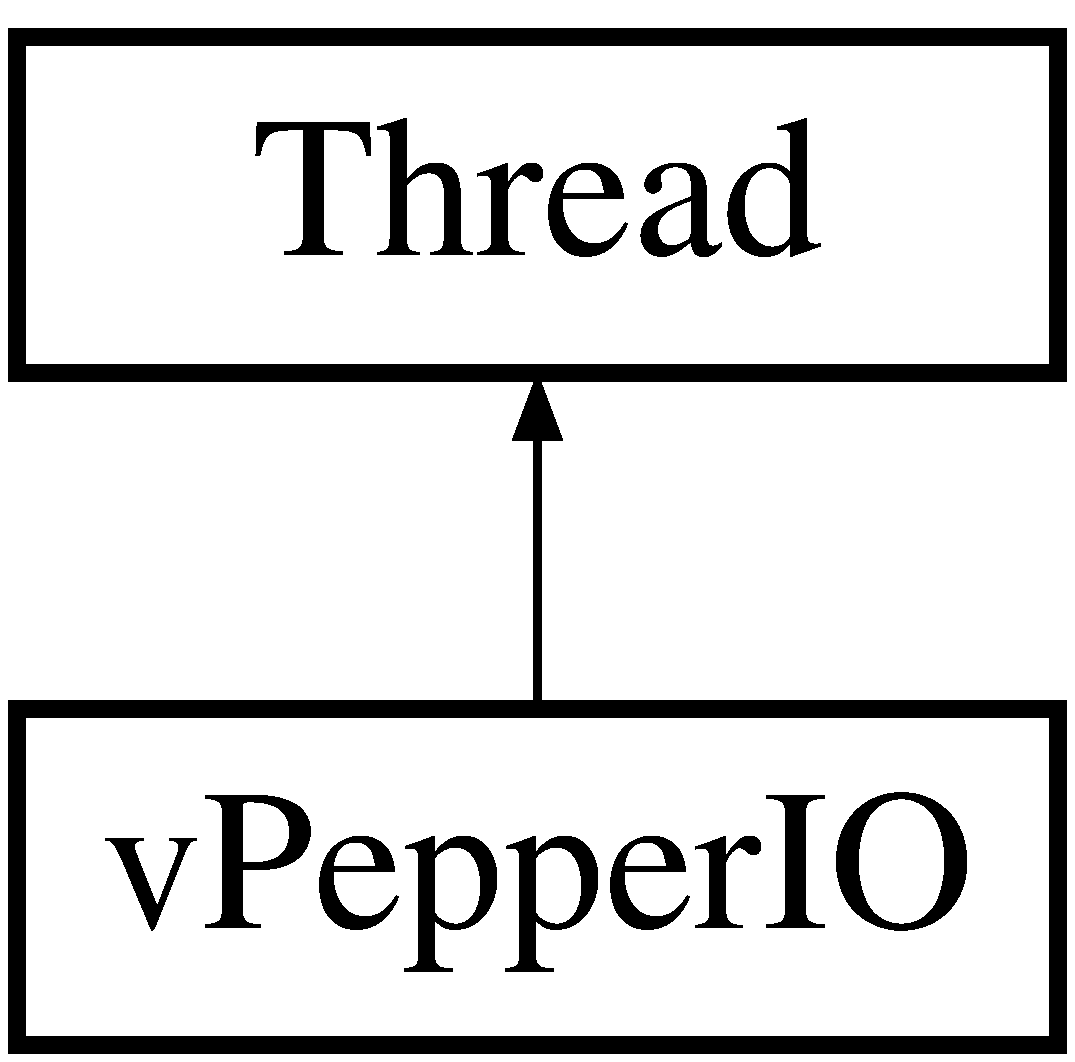
\includegraphics[height=2.000000cm]{classvPepperIO}
\end{center}
\end{figure}
\subsection*{Public Member Functions}
\begin{DoxyCompactItemize}
\item 
void {\bfseries initialise} (std\+::string name, int height, int width, int spatial\+Size, int temporal\+Size)\hypertarget{classvPepperIO_a14c1008fa51800700f00828474125044}{}\label{classvPepperIO_a14c1008fa51800700f00828474125044}

\item 
void {\bfseries run} ()\hypertarget{classvPepperIO_a625e494ecb083b3055533b953a8ca89c}{}\label{classvPepperIO_a625e494ecb083b3055533b953a8ca89c}

\item 
void {\bfseries on\+Stop} ()\hypertarget{classvPepperIO_ae54b4273e42361ad9cc515b47be0cb54}{}\label{classvPepperIO_ae54b4273e42361ad9cc515b47be0cb54}

\item 
bool {\bfseries thread\+Init} ()\hypertarget{classvPepperIO_a3bf3d088a10210d806fc4f0f0b9043a7}{}\label{classvPepperIO_a3bf3d088a10210d806fc4f0f0b9043a7}

\end{DoxyCompactItemize}


The documentation for this class was generated from the following files\+:\begin{DoxyCompactItemize}
\item 
/home/aglover/workspace/projects/event-\/driven/src/processing/v\+Pepper/include/v\+Pepper.\+h\item 
/home/aglover/workspace/projects/event-\/driven/src/processing/v\+Pepper/src/v\+Pepper.\+cpp\end{DoxyCompactItemize}

\hypertarget{classvPepperModule}{}\section{v\+Pepper\+Module Class Reference}
\label{classvPepperModule}\index{v\+Pepper\+Module@{v\+Pepper\+Module}}
Inheritance diagram for v\+Pepper\+Module\+:\begin{figure}[H]
\begin{center}
\leavevmode
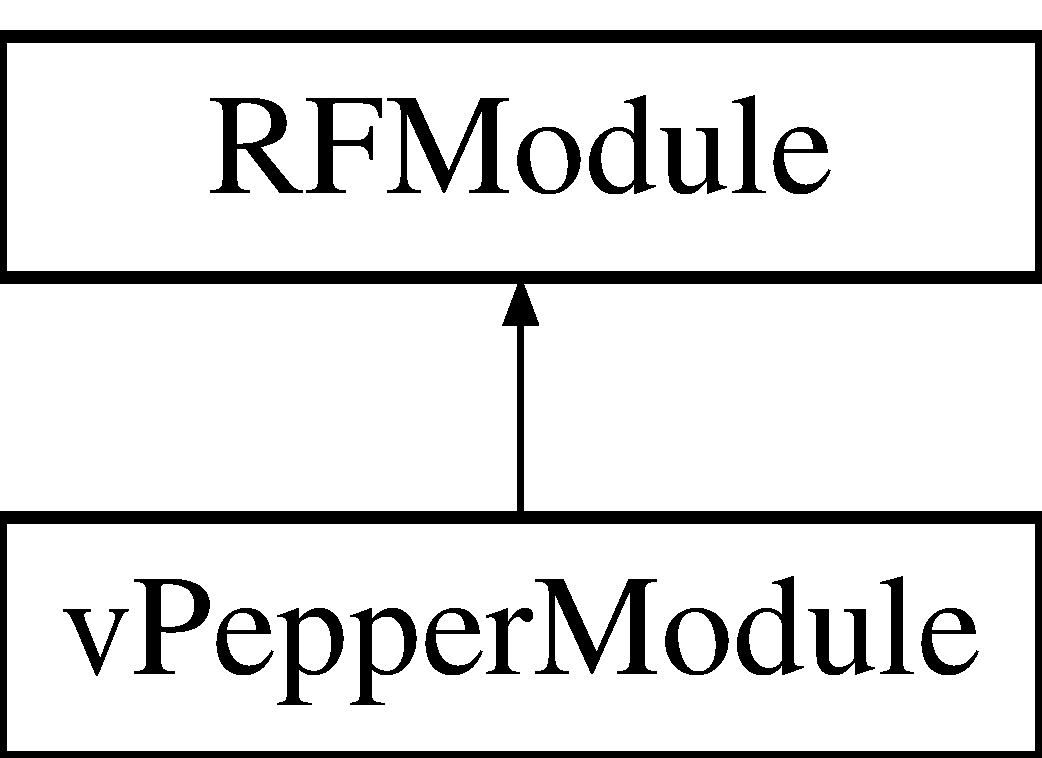
\includegraphics[height=2.000000cm]{classvPepperModule}
\end{center}
\end{figure}
\subsection*{Public Member Functions}
\begin{DoxyCompactItemize}
\item 
virtual bool {\bfseries configure} (yarp\+::os\+::\+Resource\+Finder \&rf)\hypertarget{classvPepperModule_ae52c3e869d74022e64899a10a3f8053f}{}\label{classvPepperModule_ae52c3e869d74022e64899a10a3f8053f}

\item 
virtual bool {\bfseries close} ()\hypertarget{classvPepperModule_a62f696612df2410faf03b5a369da061b}{}\label{classvPepperModule_a62f696612df2410faf03b5a369da061b}

\item 
virtual double {\bfseries get\+Period} ()\hypertarget{classvPepperModule_a4553cffc356733698afcaf17bae7cfd0}{}\label{classvPepperModule_a4553cffc356733698afcaf17bae7cfd0}

\item 
virtual bool {\bfseries update\+Module} ()\hypertarget{classvPepperModule_a07ccde7835cfc92692b35a04666f4a4e}{}\label{classvPepperModule_a07ccde7835cfc92692b35a04666f4a4e}

\end{DoxyCompactItemize}


The documentation for this class was generated from the following files\+:\begin{DoxyCompactItemize}
\item 
/home/aglover/workspace/projects/event-\/driven/src/processing/v\+Pepper/include/v\+Pepper.\+h\item 
/home/aglover/workspace/projects/event-\/driven/src/processing/v\+Pepper/src/v\+Pepper.\+cpp\end{DoxyCompactItemize}

\hypertarget{classvRepTest}{}\section{v\+Rep\+Test Class Reference}
\label{classvRepTest}\index{v\+Rep\+Test@{v\+Rep\+Test}}
Inheritance diagram for v\+Rep\+Test\+:\begin{figure}[H]
\begin{center}
\leavevmode
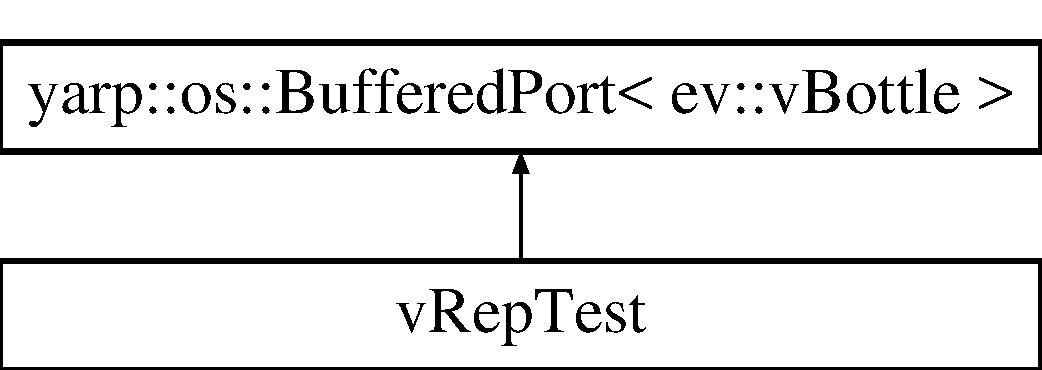
\includegraphics[height=2.000000cm]{classvRepTest}
\end{center}
\end{figure}
\subsection*{Public Member Functions}
\begin{DoxyCompactItemize}
\item 
void {\bfseries set\+Temporal\+Window} (int dt)\hypertarget{classvRepTest_afc9888397eba6894a65302b0226d81f0}{}\label{classvRepTest_afc9888397eba6894a65302b0226d81f0}

\item 
void {\bfseries set\+Fixed\+Window} (int N)\hypertarget{classvRepTest_a72524b413a72d7a56f48e1a4f2021177}{}\label{classvRepTest_a72524b413a72d7a56f48e1a4f2021177}

\item 
void {\bfseries set\+Vis\+Type} (std\+::string vis)\hypertarget{classvRepTest_aa616d24c44c0f452a42f4b02e4395967}{}\label{classvRepTest_aa616d24c44c0f452a42f4b02e4395967}

\item 
bool {\bfseries open} (const std\+::string \&name, bool strict=false)\hypertarget{classvRepTest_a02ae7ad9d91210b42178b45e3b0a7d68}{}\label{classvRepTest_a02ae7ad9d91210b42178b45e3b0a7d68}

\item 
void {\bfseries close} ()\hypertarget{classvRepTest_a95d46a88b378bb620c4ee3c0e1c7f32a}{}\label{classvRepTest_a95d46a88b378bb620c4ee3c0e1c7f32a}

\item 
void {\bfseries interrupt} ()\hypertarget{classvRepTest_aed45d04a505f13efba3cfc64bc59d795}{}\label{classvRepTest_aed45d04a505f13efba3cfc64bc59d795}

\item 
void {\bfseries on\+Read} (\hyperlink{classev_1_1vBottle}{ev\+::v\+Bottle} \&in\+Bottle)\hypertarget{classvRepTest_aea8bca9d38eed370dd7969063d93d229}{}\label{classvRepTest_aea8bca9d38eed370dd7969063d93d229}

\end{DoxyCompactItemize}


The documentation for this class was generated from the following files\+:\begin{DoxyCompactItemize}
\item 
/home/aglover/workspace/projects/event-\/driven/src/applications/reptest/include/v\+Rep\+Test.\+h\item 
/home/aglover/workspace/projects/event-\/driven/src/applications/reptest/src/v\+Rep\+Test.\+cpp\end{DoxyCompactItemize}

\hypertarget{classvRepTestHandler}{}\section{v\+Rep\+Test\+Handler Class Reference}
\label{classvRepTestHandler}\index{v\+Rep\+Test\+Handler@{v\+Rep\+Test\+Handler}}
Inheritance diagram for v\+Rep\+Test\+Handler\+:\begin{figure}[H]
\begin{center}
\leavevmode
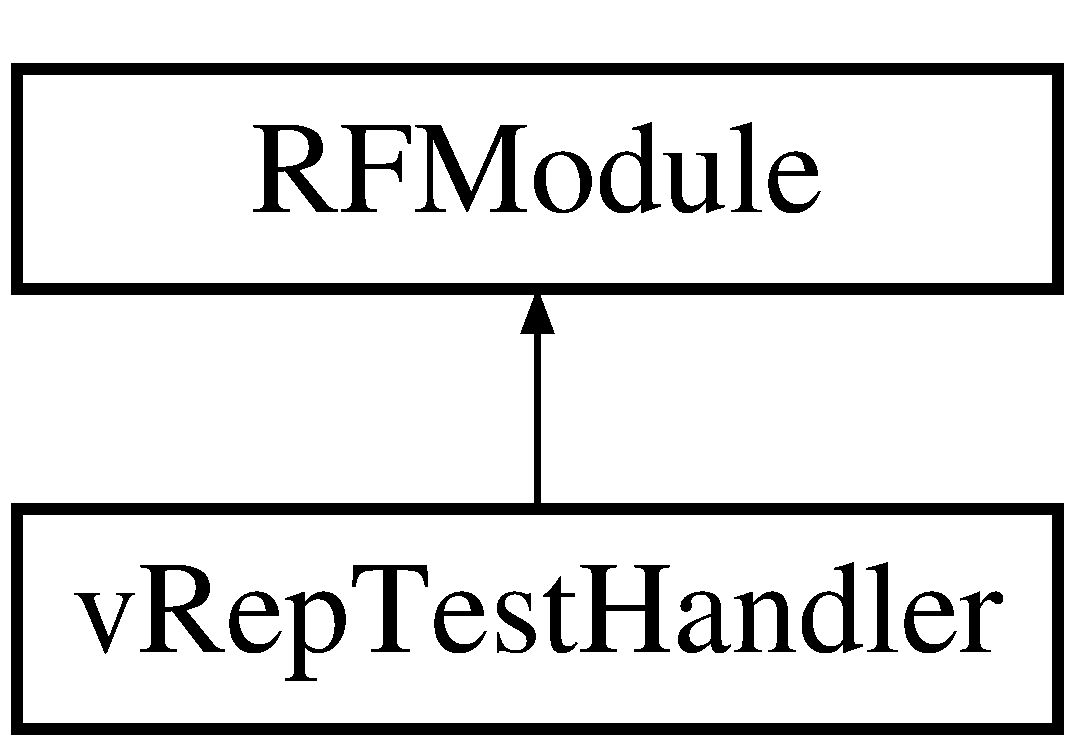
\includegraphics[height=2.000000cm]{classvRepTestHandler}
\end{center}
\end{figure}
\subsection*{Public Member Functions}
\begin{DoxyCompactItemize}
\item 
virtual bool {\bfseries configure} (yarp\+::os\+::\+Resource\+Finder \&rf)\hypertarget{classvRepTestHandler_a75d6ab4e2998eccf96b0f90b53d183f3}{}\label{classvRepTestHandler_a75d6ab4e2998eccf96b0f90b53d183f3}

\item 
virtual bool {\bfseries interrupt\+Module} ()\hypertarget{classvRepTestHandler_aa67c736991dc0601e5775b8f60b680be}{}\label{classvRepTestHandler_aa67c736991dc0601e5775b8f60b680be}

\item 
virtual bool {\bfseries close} ()\hypertarget{classvRepTestHandler_ad40900db7b64a3b8539834ff18ddc2c1}{}\label{classvRepTestHandler_ad40900db7b64a3b8539834ff18ddc2c1}

\item 
virtual double {\bfseries get\+Period} ()\hypertarget{classvRepTestHandler_a53456bbfb2edf31921b6b775b3bc1119}{}\label{classvRepTestHandler_a53456bbfb2edf31921b6b775b3bc1119}

\item 
virtual bool {\bfseries update\+Module} ()\hypertarget{classvRepTestHandler_a307f808f4e474d8b7c352e346cbda80b}{}\label{classvRepTestHandler_a307f808f4e474d8b7c352e346cbda80b}

\end{DoxyCompactItemize}


The documentation for this class was generated from the following files\+:\begin{DoxyCompactItemize}
\item 
/home/aglover/workspace/projects/event-\/driven/src/applications/reptest/include/v\+Rep\+Test.\+h\item 
/home/aglover/workspace/projects/event-\/driven/src/applications/reptest/src/v\+Rep\+Test.\+cpp\end{DoxyCompactItemize}

\hypertarget{classvSpinInterface}{}\section{v\+Spin\+Interface Class Reference}
\label{classvSpinInterface}\index{v\+Spin\+Interface@{v\+Spin\+Interface}}
Inheritance diagram for v\+Spin\+Interface\+:\begin{figure}[H]
\begin{center}
\leavevmode
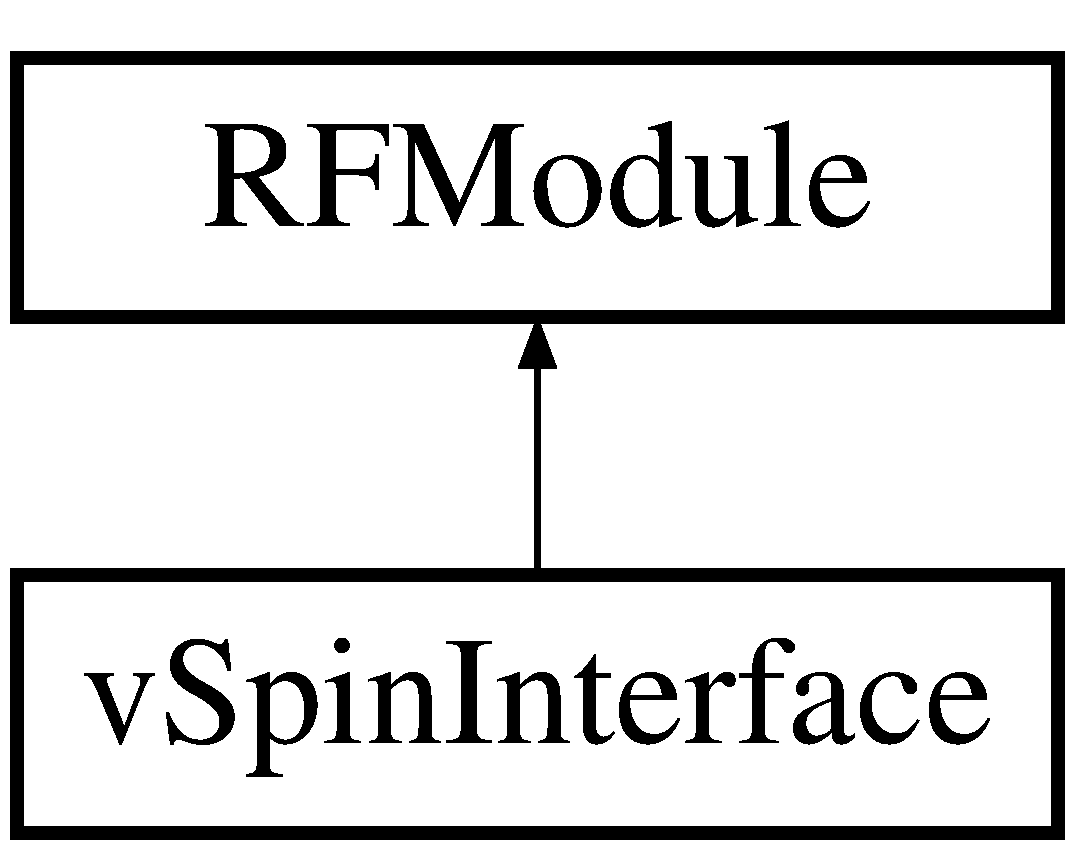
\includegraphics[height=2.000000cm]{classvSpinInterface}
\end{center}
\end{figure}
\subsection*{Public Member Functions}
\begin{DoxyCompactItemize}
\item 
virtual bool {\bfseries configure} (yarp\+::os\+::\+Resource\+Finder \&rf)\hypertarget{classvSpinInterface_afa8c4507f693729d5bf386e1190f5fbd}{}\label{classvSpinInterface_afa8c4507f693729d5bf386e1190f5fbd}

\item 
virtual bool {\bfseries interrupt\+Module} ()\hypertarget{classvSpinInterface_aa753c1ae6164708bea1fc3f01cd7f7b9}{}\label{classvSpinInterface_aa753c1ae6164708bea1fc3f01cd7f7b9}

\item 
virtual bool {\bfseries close} ()\hypertarget{classvSpinInterface_a832b19fa38602881e73cb5cea22ccb10}{}\label{classvSpinInterface_a832b19fa38602881e73cb5cea22ccb10}

\item 
virtual double {\bfseries get\+Period} ()\hypertarget{classvSpinInterface_a1addee84aa2d49ce627dd75b10a41f56}{}\label{classvSpinInterface_a1addee84aa2d49ce627dd75b10a41f56}

\item 
virtual bool {\bfseries update\+Module} ()\hypertarget{classvSpinInterface_a851d85f358a3225b18700cc2657eddff}{}\label{classvSpinInterface_a851d85f358a3225b18700cc2657eddff}

\end{DoxyCompactItemize}


The documentation for this class was generated from the following files\+:\begin{DoxyCompactItemize}
\item 
/home/aglover/workspace/projects/event-\/driven/src/hardwareio/spinterface/include/spinterface.\+h\item 
/home/aglover/workspace/projects/event-\/driven/src/hardwareio/spinterface/src/spinterface.\+cpp\end{DoxyCompactItemize}

\hypertarget{classev_1_1vSurface}{}\section{ev\+:\+:v\+Surface Class Reference}
\label{classev_1_1vSurface}\index{ev\+::v\+Surface@{ev\+::v\+Surface}}


The v\+Window class holds a list of events for a period of time as specified. Event expiry is checked each time new events are added and expired events are removed. At any point in time a copy of the current list of events can be requested.  




{\ttfamily \#include $<$v\+Window\+\_\+basic.\+h$>$}

Inheritance diagram for ev\+:\+:v\+Surface\+:\begin{figure}[H]
\begin{center}
\leavevmode
\includegraphics[height=3.000000cm]{classev_1_1vSurface}
\end{center}
\end{figure}
\subsection*{Public Member Functions}
\begin{DoxyCompactItemize}
\item 
\hyperlink{classev_1_1vSurface_afb642ce656aee165c54a2238474599c0}{v\+Surface} (int width=128, int height=128)
\begin{DoxyCompactList}\small\item\em v\+Window constructor \end{DoxyCompactList}\item 
{\bfseries v\+Surface} (const \hyperlink{classev_1_1vSurface}{v\+Surface} \&)\hypertarget{classev_1_1vSurface_a592c1c79ff294f34e28503d7c7278b8f}{}\label{classev_1_1vSurface_a592c1c79ff294f34e28503d7c7278b8f}

\item 
\hyperlink{classev_1_1vSurface}{v\+Surface} {\bfseries operator=} (const \hyperlink{classev_1_1vSurface}{v\+Surface} \&)\hypertarget{classev_1_1vSurface_af779bb51b4c9f748a0cd38117cf5e1f9}{}\label{classev_1_1vSurface_af779bb51b4c9f748a0cd38117cf5e1f9}

\item 
event$<$ \hyperlink{classev_1_1AddressEvent}{AE} $>$ \hyperlink{classev_1_1vSurface_a60d2f3d18c68d18678040cfabf6d35ea}{add\+Event} (event$<$ \hyperlink{classev_1_1AddressEvent}{AE} $>$ v)
\begin{DoxyCompactList}\small\item\em add\+Event adds an event to the window. Also checks for expired events. \end{DoxyCompactList}\item 
event$<$ \hyperlink{classev_1_1AddressEvent}{AE} $>$ \hyperlink{classev_1_1vSurface_a523c84d62fa48db30913dee7e694b895}{get\+Most\+Recent} ()
\begin{DoxyCompactList}\small\item\em get\+Most\+Recent \end{DoxyCompactList}\item 
int {\bfseries get\+Event\+Count} ()\hypertarget{classev_1_1vSurface_aa90e7d977149ee42dff7a2735b367a2b}{}\label{classev_1_1vSurface_aa90e7d977149ee42dff7a2735b367a2b}

\item 
void {\bfseries clear} ()\hypertarget{classev_1_1vSurface_a222eadfa9d900d22148d1ffb0bb68661}{}\label{classev_1_1vSurface_a222eadfa9d900d22148d1ffb0bb68661}

\item 
const v\+Queue {\bfseries get\+Surf} (int d)\hypertarget{classev_1_1vSurface_a2beddf5b5ffdbe12c1592ef8c1c742ab}{}\label{classev_1_1vSurface_a2beddf5b5ffdbe12c1592ef8c1c742ab}

\item 
const v\+Queue {\bfseries get\+Surf} (int x, int y, int d)\hypertarget{classev_1_1vSurface_af6565b2434916ebc73820fb870e6f9a9}{}\label{classev_1_1vSurface_af6565b2434916ebc73820fb870e6f9a9}

\item 
virtual const v\+Queue {\bfseries get\+Surf} (int xl, int xh, int yl, int yh)\hypertarget{classev_1_1vSurface_ae27682a1a876ef2c3b8c37c63c5a531c}{}\label{classev_1_1vSurface_ae27682a1a876ef2c3b8c37c63c5a531c}

\end{DoxyCompactItemize}
\subsection*{Protected Attributes}
\begin{DoxyCompactItemize}
\item 
std\+::vector$<$ std\+::vector$<$ event$<$ \hyperlink{classev_1_1AddressEvent}{AE} $>$ $>$ $>$ \hyperlink{classev_1_1vSurface_a157b4d26be73a1de42b0a043f12cf984}{spatial}\hypertarget{classev_1_1vSurface_a157b4d26be73a1de42b0a043f12cf984}{}\label{classev_1_1vSurface_a157b4d26be73a1de42b0a043f12cf984}

\begin{DoxyCompactList}\small\item\em for quick spatial accessing and surfacing \end{DoxyCompactList}\item 
\hyperlink{structev_1_1resolution}{resolution} {\bfseries res}\hypertarget{classev_1_1vSurface_a7ba9be674dbe03302b56306b987cff62}{}\label{classev_1_1vSurface_a7ba9be674dbe03302b56306b987cff62}

\item 
event$<$ \hyperlink{classev_1_1AddressEvent}{AE} $>$ {\bfseries most\+Recent}\hypertarget{classev_1_1vSurface_a64339e84abccbb0099e0236fa4339647}{}\label{classev_1_1vSurface_a64339e84abccbb0099e0236fa4339647}

\item 
int {\bfseries event\+Count}\hypertarget{classev_1_1vSurface_a2b6a8d84a626b8dce15597807da598fb}{}\label{classev_1_1vSurface_a2b6a8d84a626b8dce15597807da598fb}

\end{DoxyCompactItemize}


\subsection{Detailed Description}
The v\+Window class holds a list of events for a period of time as specified. Event expiry is checked each time new events are added and expired events are removed. At any point in time a copy of the current list of events can be requested. 

\subsection{Constructor \& Destructor Documentation}
\index{ev\+::v\+Surface@{ev\+::v\+Surface}!v\+Surface@{v\+Surface}}
\index{v\+Surface@{v\+Surface}!ev\+::v\+Surface@{ev\+::v\+Surface}}
\subsubsection[{\texorpdfstring{v\+Surface(int width=128, int height=128)}{vSurface(int width=128, int height=128)}}]{\setlength{\rightskip}{0pt plus 5cm}ev\+::v\+Surface\+::v\+Surface (
\begin{DoxyParamCaption}
\item[{int}]{width = {\ttfamily 128}, }
\item[{int}]{height = {\ttfamily 128}}
\end{DoxyParamCaption}
)}\hypertarget{classev_1_1vSurface_afb642ce656aee165c54a2238474599c0}{}\label{classev_1_1vSurface_afb642ce656aee165c54a2238474599c0}


v\+Window constructor 


\begin{DoxyParams}{Parameters}
{\em window\+Size} & optional time to store events (in us) \\
\hline
\end{DoxyParams}


\subsection{Member Function Documentation}
\index{ev\+::v\+Surface@{ev\+::v\+Surface}!add\+Event@{add\+Event}}
\index{add\+Event@{add\+Event}!ev\+::v\+Surface@{ev\+::v\+Surface}}
\subsubsection[{\texorpdfstring{add\+Event(event$<$ A\+E $>$ v)}{addEvent(event< AE > v)}}]{\setlength{\rightskip}{0pt plus 5cm}event$<$ {\bf AE} $>$ ev\+::v\+Surface\+::add\+Event (
\begin{DoxyParamCaption}
\item[{event$<$ {\bf AE} $>$}]{v}
\end{DoxyParamCaption}
)}\hypertarget{classev_1_1vSurface_a60d2f3d18c68d18678040cfabf6d35ea}{}\label{classev_1_1vSurface_a60d2f3d18c68d18678040cfabf6d35ea}


add\+Event adds an event to the window. Also checks for expired events. 


\begin{DoxyParams}{Parameters}
{\em event} & the event to add \\
\hline
\end{DoxyParams}
\index{ev\+::v\+Surface@{ev\+::v\+Surface}!get\+Most\+Recent@{get\+Most\+Recent}}
\index{get\+Most\+Recent@{get\+Most\+Recent}!ev\+::v\+Surface@{ev\+::v\+Surface}}
\subsubsection[{\texorpdfstring{get\+Most\+Recent()}{getMostRecent()}}]{\setlength{\rightskip}{0pt plus 5cm}event$<$ {\bf AE} $>$ ev\+::v\+Surface\+::get\+Most\+Recent (
\begin{DoxyParamCaption}
{}
\end{DoxyParamCaption}
)}\hypertarget{classev_1_1vSurface_a523c84d62fa48db30913dee7e694b895}{}\label{classev_1_1vSurface_a523c84d62fa48db30913dee7e694b895}


get\+Most\+Recent 

\begin{DoxyReturn}{Returns}

\end{DoxyReturn}


The documentation for this class was generated from the following files\+:\begin{DoxyCompactItemize}
\item 
/home/aglover/workspace/projects/event-\/driven/libraries/include/i\+Cub/eventdriven/v\+Window\+\_\+basic.\+h\item 
/home/aglover/workspace/projects/event-\/driven/libraries/src/v\+Window\+\_\+basic.\+cpp\end{DoxyCompactItemize}

\hypertarget{classev_1_1vSurface2}{}\section{ev\+:\+:v\+Surface2 Class Reference}
\label{classev_1_1vSurface2}\index{ev\+::v\+Surface2@{ev\+::v\+Surface2}}


a spatial-\/temporal surface storage data structure  




{\ttfamily \#include $<$v\+Window\+\_\+adv.\+h$>$}

Inheritance diagram for ev\+:\+:v\+Surface2\+:\begin{figure}[H]
\begin{center}
\leavevmode
\includegraphics[height=2.000000cm]{classev_1_1vSurface2}
\end{center}
\end{figure}
\subsection*{Public Member Functions}
\begin{DoxyCompactItemize}
\item 
\hyperlink{classev_1_1vSurface2_ada6aeb852479aa111b1f5ad32ac1286b}{v\+Surface2} (int \hyperlink{classev_1_1vSurface2_a1aa8027816352a15d5b9bf1f26f48e76}{width}=128, int height=128)
\begin{DoxyCompactList}\small\item\em v\+Window constructor \end{DoxyCompactList}\item 
virtual v\+Queue \hyperlink{classev_1_1vSurface2_a6dee662976048b73d7b19e45871352da}{add\+Event} (event$<$$>$ v)
\begin{DoxyCompactList}\small\item\em add\+Event adds an event to the window. Also checks for expired events. \end{DoxyCompactList}\item 
void {\bfseries fast\+Add\+Event} (event$<$$>$ v, bool only\+Add=false)\hypertarget{classev_1_1vSurface2_a311f0fb7297ee4a070755308e9271398}{}\label{classev_1_1vSurface2_a311f0fb7297ee4a070755308e9271398}

\item 
virtual v\+Queue {\bfseries remove\+Events} (event$<$$>$ to\+Add)=0\hypertarget{classev_1_1vSurface2_af35870c14a5c94dc7522bdfcf76df2cb}{}\label{classev_1_1vSurface2_af35870c14a5c94dc7522bdfcf76df2cb}

\item 
virtual void {\bfseries fast\+Remove\+Events} (event$<$$>$ to\+Add)=0\hypertarget{classev_1_1vSurface2_a956e6ab8f419554958961fbbca68029b}{}\label{classev_1_1vSurface2_a956e6ab8f419554958961fbbca68029b}

\item 
event \hyperlink{classev_1_1vSurface2_af84a860e057aea43831e8e6d16107cd4}{get\+Most\+Recent} ()
\begin{DoxyCompactList}\small\item\em get\+Most\+Recent \end{DoxyCompactList}\item 
int {\bfseries get\+Event\+Count} ()\hypertarget{classev_1_1vSurface2_a67906f1ecd7fab30f1d0f7218388234e}{}\label{classev_1_1vSurface2_a67906f1ecd7fab30f1d0f7218388234e}

\item 
v\+Queue {\bfseries get\+Everything} ()\hypertarget{classev_1_1vSurface2_a7897c4e7c034f36f86d29e14e36c2ca4}{}\label{classev_1_1vSurface2_a7897c4e7c034f36f86d29e14e36c2ca4}

\item 
v\+Queue \hyperlink{classev_1_1vSurface2_aedcc28d0ccdbc343f031506a8fa84bb0}{get\+Surf} ()
\begin{DoxyCompactList}\small\item\em get\+Window \end{DoxyCompactList}\item 
v\+Queue {\bfseries get\+Surf} (int d)\hypertarget{classev_1_1vSurface2_aaa5978b3d040e278db563495585adf86}{}\label{classev_1_1vSurface2_aaa5978b3d040e278db563495585adf86}

\item 
v\+Queue \hyperlink{classev_1_1vSurface2_a42f7a69a075225254ffddc7bb5d4d9ba}{get\+Surf} (int x, int y, int d)
\begin{DoxyCompactList}\small\item\em get\+Spatial\+Window returns Address\+Events within a spatial window \end{DoxyCompactList}\item 
v\+Queue \hyperlink{classev_1_1vSurface2_aa74adc0c56d62a6f51c2901ec209233e}{get\+Surf} (int xl, int xh, int yl, int yh)
\begin{DoxyCompactList}\small\item\em get\+Spatial\+Window returns Address\+Events within a spatial window \end{DoxyCompactList}\item 
v\+Queue {\bfseries get\+Surf\+\_\+\+Tlim} (int dt)\hypertarget{classev_1_1vSurface2_a70e292820956b12c3bc123c4e724e90a}{}\label{classev_1_1vSurface2_a70e292820956b12c3bc123c4e724e90a}

\item 
v\+Queue {\bfseries get\+Surf\+\_\+\+Tlim} (int dt, int d)\hypertarget{classev_1_1vSurface2_ad487a13d9bcd8433489fb7e7b3fa5dc8}{}\label{classev_1_1vSurface2_ad487a13d9bcd8433489fb7e7b3fa5dc8}

\item 
v\+Queue {\bfseries get\+Surf\+\_\+\+Tlim} (int dt, int x, int y, int d)\hypertarget{classev_1_1vSurface2_a53939fc4b201eaee766114982d0ae9c2}{}\label{classev_1_1vSurface2_a53939fc4b201eaee766114982d0ae9c2}

\item 
v\+Queue {\bfseries get\+Surf\+\_\+\+Tlim} (int dt, int xl, int xh, int yl, int yh)\hypertarget{classev_1_1vSurface2_a63c601ec2570dbde037c9ea92342b24b}{}\label{classev_1_1vSurface2_a63c601ec2570dbde037c9ea92342b24b}

\item 
v\+Queue {\bfseries get\+Surf\+\_\+\+Clim} (int c)\hypertarget{classev_1_1vSurface2_acb41c1eff67ff285be715f8504d37d22}{}\label{classev_1_1vSurface2_acb41c1eff67ff285be715f8504d37d22}

\item 
v\+Queue {\bfseries get\+Surf\+\_\+\+Clim} (int c, int d)\hypertarget{classev_1_1vSurface2_af9e9a30828d508f49921b02224723a36}{}\label{classev_1_1vSurface2_af9e9a30828d508f49921b02224723a36}

\item 
v\+Queue {\bfseries get\+Surf\+\_\+\+Clim} (int c, int x, int y, int d)\hypertarget{classev_1_1vSurface2_a708416f0ae3b13858f1c96e203898223}{}\label{classev_1_1vSurface2_a708416f0ae3b13858f1c96e203898223}

\item 
v\+Queue {\bfseries get\+Surf\+\_\+\+Clim} (int c, int xl, int xh, int yl, int yh)\hypertarget{classev_1_1vSurface2_a1b04ff8d8d449b054a514c092bac1145}{}\label{classev_1_1vSurface2_a1b04ff8d8d449b054a514c092bac1145}

\item 
void {\bfseries get\+Surf\+Sorted} (v\+Queue \&fillq)\hypertarget{classev_1_1vSurface2_aacd14a2e5c73e557b7b6b90a20624e23}{}\label{classev_1_1vSurface2_aacd14a2e5c73e557b7b6b90a20624e23}

\end{DoxyCompactItemize}
\subsection*{Protected Attributes}
\begin{DoxyCompactItemize}
\item 
v\+Queue \hyperlink{classev_1_1vSurface2_ad26e2a77d859924e39526fe69ad6e8bf}{q}\hypertarget{classev_1_1vSurface2_ad26e2a77d859924e39526fe69ad6e8bf}{}\label{classev_1_1vSurface2_ad26e2a77d859924e39526fe69ad6e8bf}

\begin{DoxyCompactList}\small\item\em event storage \end{DoxyCompactList}\item 
std\+::vector$<$ std\+::vector$<$ event$<$$>$ $>$ $>$ \hyperlink{classev_1_1vSurface2_aeea3647a3da9c08bd0f3bd577e6ba443}{spatial}\hypertarget{classev_1_1vSurface2_aeea3647a3da9c08bd0f3bd577e6ba443}{}\label{classev_1_1vSurface2_aeea3647a3da9c08bd0f3bd577e6ba443}

\begin{DoxyCompactList}\small\item\em for quick spatial accessing and surfacing \end{DoxyCompactList}\item 
int \hyperlink{classev_1_1vSurface2_a1aa8027816352a15d5b9bf1f26f48e76}{width}\hypertarget{classev_1_1vSurface2_a1aa8027816352a15d5b9bf1f26f48e76}{}\label{classev_1_1vSurface2_a1aa8027816352a15d5b9bf1f26f48e76}

\begin{DoxyCompactList}\small\item\em retina size \end{DoxyCompactList}\item 
int {\bfseries height}\hypertarget{classev_1_1vSurface2_a4cac3483eefdbe9e83ced2ef6bc5f7b2}{}\label{classev_1_1vSurface2_a4cac3483eefdbe9e83ced2ef6bc5f7b2}

\item 
int \hyperlink{classev_1_1vSurface2_a53cfa9932bf60007440cbf535c115222}{count}\hypertarget{classev_1_1vSurface2_a53cfa9932bf60007440cbf535c115222}{}\label{classev_1_1vSurface2_a53cfa9932bf60007440cbf535c115222}

\begin{DoxyCompactList}\small\item\em active events \end{DoxyCompactList}\end{DoxyCompactItemize}


\subsection{Detailed Description}
a spatial-\/temporal surface storage data structure 

\subsection{Constructor \& Destructor Documentation}
\index{ev\+::v\+Surface2@{ev\+::v\+Surface2}!v\+Surface2@{v\+Surface2}}
\index{v\+Surface2@{v\+Surface2}!ev\+::v\+Surface2@{ev\+::v\+Surface2}}
\subsubsection[{\texorpdfstring{v\+Surface2(int width=128, int height=128)}{vSurface2(int width=128, int height=128)}}]{\setlength{\rightskip}{0pt plus 5cm}ev\+::v\+Surface2\+::v\+Surface2 (
\begin{DoxyParamCaption}
\item[{int}]{width = {\ttfamily 128}, }
\item[{int}]{height = {\ttfamily 128}}
\end{DoxyParamCaption}
)}\hypertarget{classev_1_1vSurface2_ada6aeb852479aa111b1f5ad32ac1286b}{}\label{classev_1_1vSurface2_ada6aeb852479aa111b1f5ad32ac1286b}


v\+Window constructor 


\begin{DoxyParams}{Parameters}
{\em window\+Size} & optional time to store events (in us) \\
\hline
\end{DoxyParams}


\subsection{Member Function Documentation}
\index{ev\+::v\+Surface2@{ev\+::v\+Surface2}!add\+Event@{add\+Event}}
\index{add\+Event@{add\+Event}!ev\+::v\+Surface2@{ev\+::v\+Surface2}}
\subsubsection[{\texorpdfstring{add\+Event(event$<$$>$ v)}{addEvent(event<> v)}}]{\setlength{\rightskip}{0pt plus 5cm}v\+Queue ev\+::v\+Surface2\+::add\+Event (
\begin{DoxyParamCaption}
\item[{event$<$$>$}]{v}
\end{DoxyParamCaption}
)\hspace{0.3cm}{\ttfamily [virtual]}}\hypertarget{classev_1_1vSurface2_a6dee662976048b73d7b19e45871352da}{}\label{classev_1_1vSurface2_a6dee662976048b73d7b19e45871352da}


add\+Event adds an event to the window. Also checks for expired events. 


\begin{DoxyParams}{Parameters}
{\em event} & the event to add \\
\hline
\end{DoxyParams}


Reimplemented in \hyperlink{classev_1_1lifetimeSurface_a8fce037a13281c0e46c7d660e0ea2275}{ev\+::lifetime\+Surface}.

\index{ev\+::v\+Surface2@{ev\+::v\+Surface2}!get\+Most\+Recent@{get\+Most\+Recent}}
\index{get\+Most\+Recent@{get\+Most\+Recent}!ev\+::v\+Surface2@{ev\+::v\+Surface2}}
\subsubsection[{\texorpdfstring{get\+Most\+Recent()}{getMostRecent()}}]{\setlength{\rightskip}{0pt plus 5cm}event ev\+::v\+Surface2\+::get\+Most\+Recent (
\begin{DoxyParamCaption}
{}
\end{DoxyParamCaption}
)}\hypertarget{classev_1_1vSurface2_af84a860e057aea43831e8e6d16107cd4}{}\label{classev_1_1vSurface2_af84a860e057aea43831e8e6d16107cd4}


get\+Most\+Recent 

\begin{DoxyReturn}{Returns}

\end{DoxyReturn}
\index{ev\+::v\+Surface2@{ev\+::v\+Surface2}!get\+Surf@{get\+Surf}}
\index{get\+Surf@{get\+Surf}!ev\+::v\+Surface2@{ev\+::v\+Surface2}}
\subsubsection[{\texorpdfstring{get\+Surf()}{getSurf()}}]{\setlength{\rightskip}{0pt plus 5cm}v\+Queue ev\+::v\+Surface2\+::get\+Surf (
\begin{DoxyParamCaption}
{}
\end{DoxyParamCaption}
)}\hypertarget{classev_1_1vSurface2_aedcc28d0ccdbc343f031506a8fa84bb0}{}\label{classev_1_1vSurface2_aedcc28d0ccdbc343f031506a8fa84bb0}


get\+Window 

\begin{DoxyReturn}{Returns}

\end{DoxyReturn}
\index{ev\+::v\+Surface2@{ev\+::v\+Surface2}!get\+Surf@{get\+Surf}}
\index{get\+Surf@{get\+Surf}!ev\+::v\+Surface2@{ev\+::v\+Surface2}}
\subsubsection[{\texorpdfstring{get\+Surf(int x, int y, int d)}{getSurf(int x, int y, int d)}}]{\setlength{\rightskip}{0pt plus 5cm}v\+Queue ev\+::v\+Surface2\+::get\+Surf (
\begin{DoxyParamCaption}
\item[{int}]{x, }
\item[{int}]{y, }
\item[{int}]{d}
\end{DoxyParamCaption}
)}\hypertarget{classev_1_1vSurface2_a42f7a69a075225254ffddc7bb5d4d9ba}{}\label{classev_1_1vSurface2_a42f7a69a075225254ffddc7bb5d4d9ba}


get\+Spatial\+Window returns Address\+Events within a spatial window 


\begin{DoxyParams}{Parameters}
{\em x} & x centre \\
\hline
{\em y} & y centre \\
\hline
{\em d} & distance of the half-\/length of a square window \\
\hline
\end{DoxyParams}
\begin{DoxyReturn}{Returns}
a v\+Queue containing a copy of the events 
\end{DoxyReturn}
\index{ev\+::v\+Surface2@{ev\+::v\+Surface2}!get\+Surf@{get\+Surf}}
\index{get\+Surf@{get\+Surf}!ev\+::v\+Surface2@{ev\+::v\+Surface2}}
\subsubsection[{\texorpdfstring{get\+Surf(int xl, int xh, int yl, int yh)}{getSurf(int xl, int xh, int yl, int yh)}}]{\setlength{\rightskip}{0pt plus 5cm}v\+Queue ev\+::v\+Surface2\+::get\+Surf (
\begin{DoxyParamCaption}
\item[{int}]{xl, }
\item[{int}]{xh, }
\item[{int}]{yl, }
\item[{int}]{yh}
\end{DoxyParamCaption}
)}\hypertarget{classev_1_1vSurface2_aa74adc0c56d62a6f51c2901ec209233e}{}\label{classev_1_1vSurface2_aa74adc0c56d62a6f51c2901ec209233e}


get\+Spatial\+Window returns Address\+Events within a spatial window 


\begin{DoxyParams}{Parameters}
{\em xl} & lower x value of window \\
\hline
{\em xh} & upper x value of window \\
\hline
{\em yl} & lower y value of window \\
\hline
{\em yh} & upper y value of window \\
\hline
\end{DoxyParams}
\begin{DoxyReturn}{Returns}
a v\+Queue containing a copy of the events 
\end{DoxyReturn}


The documentation for this class was generated from the following files\+:\begin{DoxyCompactItemize}
\item 
/home/aglover/workspace/projects/event-\/driven/libraries/include/i\+Cub/eventdriven/v\+Window\+\_\+adv.\+h\item 
/home/aglover/workspace/projects/event-\/driven/libraries/src/v\+Window\+\_\+adv.\+cpp\end{DoxyCompactItemize}

\hypertarget{classev_1_1vTempWindow}{}\section{ev\+:\+:v\+Temp\+Window Class Reference}
\label{classev_1_1vTempWindow}\index{ev\+::v\+Temp\+Window@{ev\+::v\+Temp\+Window}}


store events for a fixed amount of time in a v\+Queue  




{\ttfamily \#include $<$v\+Window\+\_\+basic.\+h$>$}

Inheritance diagram for ev\+:\+:v\+Temp\+Window\+:\begin{figure}[H]
\begin{center}
\leavevmode
\includegraphics[height=2.000000cm]{classev_1_1vTempWindow}
\end{center}
\end{figure}
\subsection*{Public Member Functions}
\begin{DoxyCompactItemize}
\item 
void {\bfseries add\+Event} (event$<$$>$ v)\hypertarget{classev_1_1vTempWindow_a9499371e18cc811e2cd3e47e8e96f8ca}{}\label{classev_1_1vTempWindow_a9499371e18cc811e2cd3e47e8e96f8ca}

\item 
void {\bfseries add\+Events} (const v\+Queue \&events)\hypertarget{classev_1_1vTempWindow_a925ee62f3dff9517654fd6a9a402616b}{}\label{classev_1_1vTempWindow_a925ee62f3dff9517654fd6a9a402616b}

\item 
v\+Queue {\bfseries get\+Window} ()\hypertarget{classev_1_1vTempWindow_a40ddfc12e259c028a57d5dd188b3e2e9}{}\label{classev_1_1vTempWindow_a40ddfc12e259c028a57d5dd188b3e2e9}

\end{DoxyCompactItemize}
\subsection*{Protected Attributes}
\begin{DoxyCompactItemize}
\item 
v\+Queue \hyperlink{classev_1_1vTempWindow_abed022ad51f68443a2350fbeabbb4233}{q}\hypertarget{classev_1_1vTempWindow_abed022ad51f68443a2350fbeabbb4233}{}\label{classev_1_1vTempWindow_abed022ad51f68443a2350fbeabbb4233}

\begin{DoxyCompactList}\small\item\em event storage \end{DoxyCompactList}\item 
int \hyperlink{classev_1_1vTempWindow_a909a8f6df0014d1f318c6209223f5fad}{t\+Upper}\hypertarget{classev_1_1vTempWindow_a909a8f6df0014d1f318c6209223f5fad}{}\label{classev_1_1vTempWindow_a909a8f6df0014d1f318c6209223f5fad}

\begin{DoxyCompactList}\small\item\em precalculated thresholds \end{DoxyCompactList}\item 
int {\bfseries t\+Lower}\hypertarget{classev_1_1vTempWindow_a47845a9e47b73598e2a325c06e994bed}{}\label{classev_1_1vTempWindow_a47845a9e47b73598e2a325c06e994bed}

\end{DoxyCompactItemize}


\subsection{Detailed Description}
store events for a fixed amount of time in a v\+Queue 

The documentation for this class was generated from the following files\+:\begin{DoxyCompactItemize}
\item 
/home/aglover/workspace/projects/event-\/driven/libraries/include/i\+Cub/eventdriven/v\+Window\+\_\+basic.\+h\item 
/home/aglover/workspace/projects/event-\/driven/libraries/src/v\+Window\+\_\+basic.\+cpp\end{DoxyCompactItemize}

\hypertarget{classvTrackToRobotModule}{}\section{v\+Track\+To\+Robot\+Module Class Reference}
\label{classvTrackToRobotModule}\index{v\+Track\+To\+Robot\+Module@{v\+Track\+To\+Robot\+Module}}
Inheritance diagram for v\+Track\+To\+Robot\+Module\+:\begin{figure}[H]
\begin{center}
\leavevmode
\includegraphics[height=2.000000cm]{classvTrackToRobotModule}
\end{center}
\end{figure}
\subsection*{Public Member Functions}
\begin{DoxyCompactItemize}
\item 
virtual bool {\bfseries configure} (yarp\+::os\+::\+Resource\+Finder \&rf)\hypertarget{classvTrackToRobotModule_ac724b3b5b9a538f211b062d2adf0118d}{}\label{classvTrackToRobotModule_ac724b3b5b9a538f211b062d2adf0118d}

\item 
virtual bool {\bfseries interrupt\+Module} ()\hypertarget{classvTrackToRobotModule_a83db4c48a68b502cc18b8a2ddad56f31}{}\label{classvTrackToRobotModule_a83db4c48a68b502cc18b8a2ddad56f31}

\item 
virtual bool {\bfseries close} ()\hypertarget{classvTrackToRobotModule_af9d2b13bb4c006718d62a354f96a559a}{}\label{classvTrackToRobotModule_af9d2b13bb4c006718d62a354f96a559a}

\item 
virtual double {\bfseries get\+Period} ()\hypertarget{classvTrackToRobotModule_adcd051ae7fa4bec4cc8dd121c1f85931}{}\label{classvTrackToRobotModule_adcd051ae7fa4bec4cc8dd121c1f85931}

\item 
virtual bool {\bfseries update\+Module} ()\hypertarget{classvTrackToRobotModule_a6cb66f0717a055864f7ab4f8f0d8c132}{}\label{classvTrackToRobotModule_a6cb66f0717a055864f7ab4f8f0d8c132}

\item 
virtual bool {\bfseries respond} (const yarp\+::os\+::\+Bottle \&command, yarp\+::os\+::\+Bottle \&reply)\hypertarget{classvTrackToRobotModule_af14c10f5261e4a7790f35872f7e81361}{}\label{classvTrackToRobotModule_af14c10f5261e4a7790f35872f7e81361}

\end{DoxyCompactItemize}


The documentation for this class was generated from the following files\+:\begin{DoxyCompactItemize}
\item 
/home/aglover/workspace/projects/event-\/driven/src/applications/gaze\+Demo/include/v\+Track\+To\+Robot.\+h\item 
/home/aglover/workspace/projects/event-\/driven/src/applications/gaze\+Demo/src/v\+Track\+To\+Robot.\+cpp\end{DoxyCompactItemize}

\hypertarget{classev_1_1vtsHelper}{}\section{ev\+:\+:vts\+Helper Class Reference}
\label{classev_1_1vtsHelper}\index{ev\+::vts\+Helper@{ev\+::vts\+Helper}}


helper class to deal with timestamp conversion and wrapping  




{\ttfamily \#include $<$vts\+Helper.\+h$>$}

\subsection*{Public Member Functions}
\begin{DoxyCompactItemize}
\item 
unsigned long int {\bfseries operator()} (int timestamp)\hypertarget{classev_1_1vtsHelper_a399c3a719f7544209ba77f442c97c135}{}\label{classev_1_1vtsHelper_a399c3a719f7544209ba77f442c97c135}

\item 
unsigned long int {\bfseries current\+Time} ()\hypertarget{classev_1_1vtsHelper_ab8b7f4f4240f2a0f0279bda5f5f2caff}{}\label{classev_1_1vtsHelper_ab8b7f4f4240f2a0f0279bda5f5f2caff}

\end{DoxyCompactItemize}
\subsection*{Static Public Member Functions}
\begin{DoxyCompactItemize}
\item 
static long int {\bfseries max\+Stamp} ()\hypertarget{classev_1_1vtsHelper_aa7f1c13eb051773e9413b52bb52caad0}{}\label{classev_1_1vtsHelper_aa7f1c13eb051773e9413b52bb52caad0}

\item 
static double {\bfseries tstosecs} ()\hypertarget{classev_1_1vtsHelper_a07d0dc3cd7743eff7d594e838ae23a01}{}\label{classev_1_1vtsHelper_a07d0dc3cd7743eff7d594e838ae23a01}

\end{DoxyCompactItemize}
\subsection*{Static Public Attributes}
\begin{DoxyCompactItemize}
\item 
static long int {\bfseries max\+\_\+stamp} = 16777215\hypertarget{classev_1_1vtsHelper_a90d44d8ec100b8bd154bf7c87e895d17}{}\label{classev_1_1vtsHelper_a90d44d8ec100b8bd154bf7c87e895d17}

\item 
static double {\bfseries tsscaler} = 0.\+000000128\hypertarget{classev_1_1vtsHelper_ad3ad427d18c24f9655bbc73295abf678}{}\label{classev_1_1vtsHelper_ad3ad427d18c24f9655bbc73295abf678}

\item 
static double {\bfseries vtsscaler} = 7812500\hypertarget{classev_1_1vtsHelper_afa2dd46ae7113668bc6ebea88ab8fa11}{}\label{classev_1_1vtsHelper_afa2dd46ae7113668bc6ebea88ab8fa11}

\end{DoxyCompactItemize}


\subsection{Detailed Description}
helper class to deal with timestamp conversion and wrapping 

The documentation for this class was generated from the following files\+:\begin{DoxyCompactItemize}
\item 
/home/aglover/workspace/projects/event-\/driven/libraries/include/i\+Cub/eventdriven/vts\+Helper.\+h\item 
/home/aglover/workspace/projects/event-\/driven/libraries/src/vts\+Helper.\+cpp\end{DoxyCompactItemize}

\hypertarget{classvUndistortModule}{}\section{v\+Undistort\+Module Class Reference}
\label{classvUndistortModule}\index{v\+Undistort\+Module@{v\+Undistort\+Module}}
Inheritance diagram for v\+Undistort\+Module\+:\begin{figure}[H]
\begin{center}
\leavevmode
\includegraphics[height=2.000000cm]{classvUndistortModule}
\end{center}
\end{figure}
\subsection*{Public Member Functions}
\begin{DoxyCompactItemize}
\item 
virtual bool {\bfseries configure} (yarp\+::os\+::\+Resource\+Finder \&rf)\hypertarget{classvUndistortModule_a9f4fce79ccdc9e9b3b2269c4d94beb22}{}\label{classvUndistortModule_a9f4fce79ccdc9e9b3b2269c4d94beb22}

\item 
virtual bool {\bfseries interrupt\+Module} ()\hypertarget{classvUndistortModule_ab552bfdeddb57cb1cb332169761571d8}{}\label{classvUndistortModule_ab552bfdeddb57cb1cb332169761571d8}

\item 
virtual bool {\bfseries close} ()\hypertarget{classvUndistortModule_a03d2de14720d332b0bbafe5b200f3ce0}{}\label{classvUndistortModule_a03d2de14720d332b0bbafe5b200f3ce0}

\item 
virtual bool {\bfseries respond} (const yarp\+::os\+::\+Bottle \&command, yarp\+::os\+::\+Bottle \&reply)\hypertarget{classvUndistortModule_a11c58860f7bcd6783d8265b55b8a4fe9}{}\label{classvUndistortModule_a11c58860f7bcd6783d8265b55b8a4fe9}

\item 
virtual double {\bfseries get\+Period} ()\hypertarget{classvUndistortModule_a8ec64be6e169a66a5c68aedb3f8618f0}{}\label{classvUndistortModule_a8ec64be6e169a66a5c68aedb3f8618f0}

\item 
virtual bool {\bfseries update\+Module} ()\hypertarget{classvUndistortModule_a68a6946ee4bb8197ec555cf3d2f3b657}{}\label{classvUndistortModule_a68a6946ee4bb8197ec555cf3d2f3b657}

\end{DoxyCompactItemize}


The documentation for this class was generated from the following files\+:\begin{DoxyCompactItemize}
\item 
/home/aglover/workspace/projects/event-\/driven/src/processing/v\+Undistort\+Cam/include/v\+Undistort\+Cam.\+h\item 
/home/aglover/workspace/projects/event-\/driven/src/processing/v\+Undistort\+Cam/src/v\+Undistort\+Cam.\+cpp\end{DoxyCompactItemize}

\hypertarget{classvVergenceManager}{}\section{v\+Vergence\+Manager Class Reference}
\label{classvVergenceManager}\index{v\+Vergence\+Manager@{v\+Vergence\+Manager}}
Inheritance diagram for v\+Vergence\+Manager\+:\begin{figure}[H]
\begin{center}
\leavevmode
\includegraphics[height=2.000000cm]{classvVergenceManager}
\end{center}
\end{figure}
\subsection*{Public Member Functions}
\begin{DoxyCompactItemize}
\item 
{\bfseries v\+Vergence\+Manager} (int width, int height, int n\+Events, int number\+Ori, int number\+Phases, int max\+Disparity, double stds\+Per\+Lambda, double threshold)\hypertarget{classvVergenceManager_a1a6f52d8f4cb48555ce78a46f18fb6bd}{}\label{classvVergenceManager_a1a6f52d8f4cb48555ce78a46f18fb6bd}

\item 
void {\bfseries start\+Verging} ()\hypertarget{classvVergenceManager_ab81f067e0c77e52466d0fa286f2998eb}{}\label{classvVergenceManager_ab81f067e0c77e52466d0fa286f2998eb}

\item 
void {\bfseries reset\+Vergence} ()\hypertarget{classvVergenceManager_ae9a760ac725054c4d7a54c59043c2e5d}{}\label{classvVergenceManager_ae9a760ac725054c4d7a54c59043c2e5d}

\item 
bool {\bfseries open} (const std\+::string \&name, bool strictness)\hypertarget{classvVergenceManager_a426ca10e1feef76e4290c697eced6b47}{}\label{classvVergenceManager_a426ca10e1feef76e4290c697eced6b47}

\item 
void {\bfseries close} ()\hypertarget{classvVergenceManager_a9b8f1b2639f222fc280c20719f8959af}{}\label{classvVergenceManager_a9b8f1b2639f222fc280c20719f8959af}

\item 
void {\bfseries interrupt} ()\hypertarget{classvVergenceManager_aa6cc4cf8270c835e8bbe86ef382eb3dd}{}\label{classvVergenceManager_aa6cc4cf8270c835e8bbe86ef382eb3dd}

\item 
void {\bfseries setkp} (double kp)\hypertarget{classvVergenceManager_a1d4eff6ba5353bf2fcffaae2c9bab539}{}\label{classvVergenceManager_a1d4eff6ba5353bf2fcffaae2c9bab539}

\item 
void {\bfseries setkd} (double kd)\hypertarget{classvVergenceManager_a9b51d753f0f118faa786361b6853f4b5}{}\label{classvVergenceManager_a9b51d753f0f118faa786361b6853f4b5}

\item 
void {\bfseries on\+Read} (\hyperlink{classev_1_1vBottle}{ev\+::v\+Bottle} \&bot)\hypertarget{classvVergenceManager_a19c62351b2585b6745b171f5a2a36503}{}\label{classvVergenceManager_a19c62351b2585b6745b171f5a2a36503}

\end{DoxyCompactItemize}


The documentation for this class was generated from the following files\+:\begin{DoxyCompactItemize}
\item 
/home/aglover/workspace/projects/event-\/driven/src/applications/vergence\+Demo/vergence\+Controller/include/vergence\+Controller.\+h\item 
/home/aglover/workspace/projects/event-\/driven/src/applications/vergence\+Demo/vergence\+Controller/src/vergence\+Controller.\+cpp\end{DoxyCompactItemize}

\hypertarget{classvVergenceModule}{}\section{v\+Vergence\+Module Class Reference}
\label{classvVergenceModule}\index{v\+Vergence\+Module@{v\+Vergence\+Module}}
Inheritance diagram for v\+Vergence\+Module\+:\begin{figure}[H]
\begin{center}
\leavevmode
\includegraphics[height=2.000000cm]{classvVergenceModule}
\end{center}
\end{figure}
\subsection*{Public Member Functions}
\begin{DoxyCompactItemize}
\item 
virtual bool {\bfseries configure} (yarp\+::os\+::\+Resource\+Finder \&rf)\hypertarget{classvVergenceModule_af5adccf2e4e683156898b873c0c08988}{}\label{classvVergenceModule_af5adccf2e4e683156898b873c0c08988}

\item 
virtual bool {\bfseries interrupt\+Module} ()\hypertarget{classvVergenceModule_aaeb20d7a6c54c7e062e81449909f7108}{}\label{classvVergenceModule_aaeb20d7a6c54c7e062e81449909f7108}

\item 
virtual bool {\bfseries close} ()\hypertarget{classvVergenceModule_a3a1ff9fa51ab9f0ceba8e64bcef3cd83}{}\label{classvVergenceModule_a3a1ff9fa51ab9f0ceba8e64bcef3cd83}

\item 
virtual bool {\bfseries respond} (const yarp\+::os\+::\+Bottle \&command, yarp\+::os\+::\+Bottle \&reply)\hypertarget{classvVergenceModule_a43c817d4e7da3d93d4ee82b2b2c0441c}{}\label{classvVergenceModule_a43c817d4e7da3d93d4ee82b2b2c0441c}

\item 
virtual double {\bfseries get\+Period} ()\hypertarget{classvVergenceModule_a42f1b19c3560a5a474a78278c0263338}{}\label{classvVergenceModule_a42f1b19c3560a5a474a78278c0263338}

\item 
virtual bool {\bfseries update\+Module} ()\hypertarget{classvVergenceModule_a068dd0cb890c7c6c868ffa3f58866837}{}\label{classvVergenceModule_a068dd0cb890c7c6c868ffa3f58866837}

\end{DoxyCompactItemize}


The documentation for this class was generated from the following files\+:\begin{DoxyCompactItemize}
\item 
/home/aglover/workspace/projects/event-\/driven/src/applications/vergence\+Demo/vergence\+Controller/include/vergence\+Controller.\+h\item 
/home/aglover/workspace/projects/event-\/driven/src/applications/vergence\+Demo/vergence\+Controller/src/vergence\+Controller.\+cpp\end{DoxyCompactItemize}

\hypertarget{classyarp2device}{}\section{yarp2device Class Reference}
\label{classyarp2device}\index{yarp2device@{yarp2device}}
Inheritance diagram for yarp2device\+:\begin{figure}[H]
\begin{center}
\leavevmode
\includegraphics[height=2.000000cm]{classyarp2device}
\end{center}
\end{figure}
\subsection*{Public Member Functions}
\begin{DoxyCompactItemize}
\item 
bool {\bfseries initialise} (std\+::string module\+Name, std\+::string device\+Name)\hypertarget{classyarp2device_ab25c91e26d75cad2b01544040aa46b7b}{}\label{classyarp2device_ab25c91e26d75cad2b01544040aa46b7b}

\item 
bool {\bfseries init} ()\hypertarget{classyarp2device_a56b9560746d5dec6168f62426b302598}{}\label{classyarp2device_a56b9560746d5dec6168f62426b302598}

\item 
void {\bfseries close} ()\hypertarget{classyarp2device_a4031dba4c05576ca4f444fe496fd1f42}{}\label{classyarp2device_a4031dba4c05576ca4f444fe496fd1f42}

\item 
void {\bfseries on\+Read} (\hyperlink{classev_1_1vBottle}{ev\+::v\+Bottle} \&bot)\hypertarget{classyarp2device_a52d2819114122ec00c41b31b2842c608}{}\label{classyarp2device_a52d2819114122ec00c41b31b2842c608}

\item 
void {\bfseries interrupt} ()\hypertarget{classyarp2device_ad2c4ae1fdb9839805c806d0084fdd20a}{}\label{classyarp2device_ad2c4ae1fdb9839805c806d0084fdd20a}

\end{DoxyCompactItemize}


The documentation for this class was generated from the following files\+:\begin{DoxyCompactItemize}
\item 
/home/aglover/workspace/projects/event-\/driven/src/hardwareio/zynq\+Grabber/include/yarp\+Interface.\+h\item 
/home/aglover/workspace/projects/event-\/driven/src/hardwareio/zynq\+Grabber/src/yarp\+Interface.\+cpp\end{DoxyCompactItemize}

\hypertarget{classYARPspinI}{}\section{Y\+A\+R\+PspinI Class Reference}
\label{classYARPspinI}\index{Y\+A\+R\+PspinI@{Y\+A\+R\+PspinI}}
Inheritance diagram for Y\+A\+R\+PspinI\+:\begin{figure}[H]
\begin{center}
\leavevmode
\includegraphics[height=2.000000cm]{classYARPspinI}
\end{center}
\end{figure}
\subsection*{Public Member Functions}
\begin{DoxyCompactItemize}
\item 
bool {\bfseries open} (const std\+::string \&name)\hypertarget{classYARPspinI_a749cd07632d7e3cd08846457e2d6be2e}{}\label{classYARPspinI_a749cd07632d7e3cd08846457e2d6be2e}

\item 
void {\bfseries close} ()\hypertarget{classYARPspinI_a6955f4744c185dd870b32ad17ddd75ef}{}\label{classYARPspinI_a6955f4744c185dd870b32ad17ddd75ef}

\item 
void {\bfseries interrupt} ()\hypertarget{classYARPspinI_a9340f1b20136adad3392c155393506ac}{}\label{classYARPspinI_a9340f1b20136adad3392c155393506ac}

\item 
void {\bfseries attach\+E\+I\+E\+I\+O\+Sender} (spinnio\+::\+E\+I\+E\+I\+O\+Sender $\ast$)\hypertarget{classYARPspinI_a6480c2630a974de7af8501ef2e2b9068}{}\label{classYARPspinI_a6480c2630a974de7af8501ef2e2b9068}

\item 
void {\bfseries on\+Read} (\hyperlink{classev_1_1vBottle}{ev\+::v\+Bottle} \&bot)\hypertarget{classYARPspinI_af965467765329a090b8e5153b1f01112}{}\label{classYARPspinI_af965467765329a090b8e5153b1f01112}

\end{DoxyCompactItemize}


The documentation for this class was generated from the following files\+:\begin{DoxyCompactItemize}
\item 
/home/aglover/workspace/projects/event-\/driven/src/hardwareio/spinterface/include/spinterface.\+h\item 
/home/aglover/workspace/projects/event-\/driven/src/hardwareio/spinterface/src/spinterface.\+cpp\end{DoxyCompactItemize}

\hypertarget{classYARPspinIO}{}\section{Y\+A\+R\+Pspin\+IO Class Reference}
\label{classYARPspinIO}\index{Y\+A\+R\+Pspin\+IO@{Y\+A\+R\+Pspin\+IO}}
Inheritance diagram for Y\+A\+R\+Pspin\+IO\+:\begin{figure}[H]
\begin{center}
\leavevmode
\includegraphics[height=2.000000cm]{classYARPspinIO}
\end{center}
\end{figure}
\subsection*{Public Member Functions}
\begin{DoxyCompactItemize}
\item 
bool {\bfseries open} (const std\+::string \&name)\hypertarget{classYARPspinIO_ac99ae5b0b8d9308da9a8aa76dd8b7cf6}{}\label{classYARPspinIO_ac99ae5b0b8d9308da9a8aa76dd8b7cf6}

\item 
void {\bfseries close} ()\hypertarget{classYARPspinIO_afbaa4ae29db56e010b1801a9c428386b}{}\label{classYARPspinIO_afbaa4ae29db56e010b1801a9c428386b}

\item 
void {\bfseries interrupt} ()\hypertarget{classYARPspinIO_ad00a2c121cbd513dd32726a26b15bef6}{}\label{classYARPspinIO_ad00a2c121cbd513dd32726a26b15bef6}

\item 
void {\bfseries attach\+E\+I\+E\+I\+Omodules} (spinnio\+::\+E\+I\+E\+I\+O\+Sender $\ast$spin\+Sender\+Ptr, spinnio\+::\+E\+I\+E\+I\+O\+Receiver $\ast$spin\+Receiver\+Ptr)\hypertarget{classYARPspinIO_af51eb6763550906becdf20b596c0adf9}{}\label{classYARPspinIO_af51eb6763550906becdf20b596c0adf9}

\item 
void {\bfseries on\+Read} (\hyperlink{classev_1_1vBottle}{ev\+::v\+Bottle} \&inbottle)\hypertarget{classYARPspinIO_a6f6002f899bdee449f5a695ac6f45dcb}{}\label{classYARPspinIO_a6f6002f899bdee449f5a695ac6f45dcb}

\end{DoxyCompactItemize}


The documentation for this class was generated from the following files\+:\begin{DoxyCompactItemize}
\item 
/home/aglover/workspace/projects/event-\/driven/src/hardwareio/spinterface/include/spinterface.\+h\item 
/home/aglover/workspace/projects/event-\/driven/src/hardwareio/spinterface/src/spinterface.\+cpp\end{DoxyCompactItemize}

\hypertarget{classYARPspinO}{}\section{Y\+A\+R\+PspinO Class Reference}
\label{classYARPspinO}\index{Y\+A\+R\+PspinO@{Y\+A\+R\+PspinO}}
Inheritance diagram for Y\+A\+R\+PspinO\+:\begin{figure}[H]
\begin{center}
\leavevmode
\includegraphics[height=2.000000cm]{classYARPspinO}
\end{center}
\end{figure}
\subsection*{Public Member Functions}
\begin{DoxyCompactItemize}
\item 
bool {\bfseries init\+Thread} (std\+::string module\+Name, spinnio\+::\+E\+I\+E\+I\+O\+Receiver $\ast$spin\+Receiver\+Ptr)\hypertarget{classYARPspinO_a6c43538e8a723f5d737b6bb7b67f6552}{}\label{classYARPspinO_a6c43538e8a723f5d737b6bb7b67f6552}

\item 
void {\bfseries run} ()\hypertarget{classYARPspinO_aff0148bb4f1b5a40122657ecc2cb7561}{}\label{classYARPspinO_aff0148bb4f1b5a40122657ecc2cb7561}

\item 
void {\bfseries thread\+Release} ()\hypertarget{classYARPspinO_a2e5c1ad532978c130c87b8159c2a3a0c}{}\label{classYARPspinO_a2e5c1ad532978c130c87b8159c2a3a0c}

\end{DoxyCompactItemize}


The documentation for this class was generated from the following files\+:\begin{DoxyCompactItemize}
\item 
/home/aglover/workspace/projects/event-\/driven/src/hardwareio/spinterface/include/spinterface.\+h\item 
/home/aglover/workspace/projects/event-\/driven/src/hardwareio/spinterface/src/spinterface.\+cpp\end{DoxyCompactItemize}

\hypertarget{classzynqGrabberModule}{}\section{zynq\+Grabber\+Module Class Reference}
\label{classzynqGrabberModule}\index{zynq\+Grabber\+Module@{zynq\+Grabber\+Module}}
Inheritance diagram for zynq\+Grabber\+Module\+:\begin{figure}[H]
\begin{center}
\leavevmode
\includegraphics[height=2.000000cm]{classzynqGrabberModule}
\end{center}
\end{figure}
\subsection*{Public Member Functions}
\begin{DoxyCompactItemize}
\item 
bool {\bfseries configure} (yarp\+::os\+::\+Resource\+Finder \&rf)\hypertarget{classzynqGrabberModule_a2733856709df020d264750ce5afbe552}{}\label{classzynqGrabberModule_a2733856709df020d264750ce5afbe552}

\item 
bool {\bfseries interrupt\+Module} ()\hypertarget{classzynqGrabberModule_aa33152e027843920826ea02f323df8dd}{}\label{classzynqGrabberModule_aa33152e027843920826ea02f323df8dd}

\item 
bool {\bfseries close} ()\hypertarget{classzynqGrabberModule_ae687b7063d3974a71a27a4cae8104480}{}\label{classzynqGrabberModule_ae687b7063d3974a71a27a4cae8104480}

\item 
bool {\bfseries respond} (const yarp\+::os\+::\+Bottle \&command, yarp\+::os\+::\+Bottle \&reply)\hypertarget{classzynqGrabberModule_afb439f66ef1786b6b503597dd6e74f33}{}\label{classzynqGrabberModule_afb439f66ef1786b6b503597dd6e74f33}

\item 
double {\bfseries get\+Period} ()\hypertarget{classzynqGrabberModule_a584429a662fd6eb0b11d77294c1b40a5}{}\label{classzynqGrabberModule_a584429a662fd6eb0b11d77294c1b40a5}

\item 
bool {\bfseries update\+Module} ()\hypertarget{classzynqGrabberModule_a53679eefbe74aa164fde84f9381450bc}{}\label{classzynqGrabberModule_a53679eefbe74aa164fde84f9381450bc}

\end{DoxyCompactItemize}


The documentation for this class was generated from the following files\+:\begin{DoxyCompactItemize}
\item 
/home/aglover/workspace/projects/event-\/driven/src/hardwareio/zynq\+Grabber/include/zynq\+Grabber\+Module.\+h\item 
/home/aglover/workspace/projects/event-\/driven/src/hardwareio/zynq\+Grabber/src/zynq\+Grabber\+Module.\+cpp\end{DoxyCompactItemize}

%--- End generated contents ---

% Index
\backmatter
\newpage
\phantomsection
\clearemptydoublepage
\addcontentsline{toc}{chapter}{Index}
\printindex

\end{document}
